\documentclass[]{book}
\usepackage{lmodern}
\usepackage{amssymb,amsmath}
\usepackage{ifxetex,ifluatex}
\usepackage{fixltx2e} % provides \textsubscript
\ifnum 0\ifxetex 1\fi\ifluatex 1\fi=0 % if pdftex
  \usepackage[T1]{fontenc}
  \usepackage[utf8]{inputenc}
\else % if luatex or xelatex
  \ifxetex
    \usepackage{mathspec}
  \else
    \usepackage{fontspec}
  \fi
  \defaultfontfeatures{Ligatures=TeX,Scale=MatchLowercase}
\fi
% use upquote if available, for straight quotes in verbatim environments
\IfFileExists{upquote.sty}{\usepackage{upquote}}{}
% use microtype if available
\IfFileExists{microtype.sty}{%
\usepackage{microtype}
\UseMicrotypeSet[protrusion]{basicmath} % disable protrusion for tt fonts
}{}
\usepackage[margin=1in]{geometry}
\usepackage{hyperref}
\hypersetup{unicode=true,
            pdftitle={Multidimensional poverty measurement: A statistical approach with applications},
            pdfauthor={Héctor Nájera and others...},
            pdfborder={0 0 0},
            breaklinks=true}
\urlstyle{same}  % don't use monospace font for urls
\usepackage{color}
\usepackage{fancyvrb}
\newcommand{\VerbBar}{|}
\newcommand{\VERB}{\Verb[commandchars=\\\{\}]}
\DefineVerbatimEnvironment{Highlighting}{Verbatim}{commandchars=\\\{\}}
% Add ',fontsize=\small' for more characters per line
\usepackage{framed}
\definecolor{shadecolor}{RGB}{248,248,248}
\newenvironment{Shaded}{\begin{snugshade}}{\end{snugshade}}
\newcommand{\AlertTok}[1]{\textcolor[rgb]{0.94,0.16,0.16}{#1}}
\newcommand{\AnnotationTok}[1]{\textcolor[rgb]{0.56,0.35,0.01}{\textbf{\textit{#1}}}}
\newcommand{\AttributeTok}[1]{\textcolor[rgb]{0.77,0.63,0.00}{#1}}
\newcommand{\BaseNTok}[1]{\textcolor[rgb]{0.00,0.00,0.81}{#1}}
\newcommand{\BuiltInTok}[1]{#1}
\newcommand{\CharTok}[1]{\textcolor[rgb]{0.31,0.60,0.02}{#1}}
\newcommand{\CommentTok}[1]{\textcolor[rgb]{0.56,0.35,0.01}{\textit{#1}}}
\newcommand{\CommentVarTok}[1]{\textcolor[rgb]{0.56,0.35,0.01}{\textbf{\textit{#1}}}}
\newcommand{\ConstantTok}[1]{\textcolor[rgb]{0.00,0.00,0.00}{#1}}
\newcommand{\ControlFlowTok}[1]{\textcolor[rgb]{0.13,0.29,0.53}{\textbf{#1}}}
\newcommand{\DataTypeTok}[1]{\textcolor[rgb]{0.13,0.29,0.53}{#1}}
\newcommand{\DecValTok}[1]{\textcolor[rgb]{0.00,0.00,0.81}{#1}}
\newcommand{\DocumentationTok}[1]{\textcolor[rgb]{0.56,0.35,0.01}{\textbf{\textit{#1}}}}
\newcommand{\ErrorTok}[1]{\textcolor[rgb]{0.64,0.00,0.00}{\textbf{#1}}}
\newcommand{\ExtensionTok}[1]{#1}
\newcommand{\FloatTok}[1]{\textcolor[rgb]{0.00,0.00,0.81}{#1}}
\newcommand{\FunctionTok}[1]{\textcolor[rgb]{0.00,0.00,0.00}{#1}}
\newcommand{\ImportTok}[1]{#1}
\newcommand{\InformationTok}[1]{\textcolor[rgb]{0.56,0.35,0.01}{\textbf{\textit{#1}}}}
\newcommand{\KeywordTok}[1]{\textcolor[rgb]{0.13,0.29,0.53}{\textbf{#1}}}
\newcommand{\NormalTok}[1]{#1}
\newcommand{\OperatorTok}[1]{\textcolor[rgb]{0.81,0.36,0.00}{\textbf{#1}}}
\newcommand{\OtherTok}[1]{\textcolor[rgb]{0.56,0.35,0.01}{#1}}
\newcommand{\PreprocessorTok}[1]{\textcolor[rgb]{0.56,0.35,0.01}{\textit{#1}}}
\newcommand{\RegionMarkerTok}[1]{#1}
\newcommand{\SpecialCharTok}[1]{\textcolor[rgb]{0.00,0.00,0.00}{#1}}
\newcommand{\SpecialStringTok}[1]{\textcolor[rgb]{0.31,0.60,0.02}{#1}}
\newcommand{\StringTok}[1]{\textcolor[rgb]{0.31,0.60,0.02}{#1}}
\newcommand{\VariableTok}[1]{\textcolor[rgb]{0.00,0.00,0.00}{#1}}
\newcommand{\VerbatimStringTok}[1]{\textcolor[rgb]{0.31,0.60,0.02}{#1}}
\newcommand{\WarningTok}[1]{\textcolor[rgb]{0.56,0.35,0.01}{\textbf{\textit{#1}}}}
\usepackage{longtable,booktabs}
\usepackage{graphicx,grffile}
\makeatletter
\def\maxwidth{\ifdim\Gin@nat@width>\linewidth\linewidth\else\Gin@nat@width\fi}
\def\maxheight{\ifdim\Gin@nat@height>\textheight\textheight\else\Gin@nat@height\fi}
\makeatother
% Scale images if necessary, so that they will not overflow the page
% margins by default, and it is still possible to overwrite the defaults
% using explicit options in \includegraphics[width, height, ...]{}
\setkeys{Gin}{width=\maxwidth,height=\maxheight,keepaspectratio}
\IfFileExists{parskip.sty}{%
\usepackage{parskip}
}{% else
\setlength{\parindent}{0pt}
\setlength{\parskip}{6pt plus 2pt minus 1pt}
}
\setlength{\emergencystretch}{3em}  % prevent overfull lines
\providecommand{\tightlist}{%
  \setlength{\itemsep}{0pt}\setlength{\parskip}{0pt}}
\setcounter{secnumdepth}{5}
% Redefines (sub)paragraphs to behave more like sections
\ifx\paragraph\undefined\else
\let\oldparagraph\paragraph
\renewcommand{\paragraph}[1]{\oldparagraph{#1}\mbox{}}
\fi
\ifx\subparagraph\undefined\else
\let\oldsubparagraph\subparagraph
\renewcommand{\subparagraph}[1]{\oldsubparagraph{#1}\mbox{}}
\fi

%%% Use protect on footnotes to avoid problems with footnotes in titles
\let\rmarkdownfootnote\footnote%
\def\footnote{\protect\rmarkdownfootnote}

%%% Change title format to be more compact
\usepackage{titling}

% Create subtitle command for use in maketitle
\providecommand{\subtitle}[1]{
  \posttitle{
    \begin{center}\large#1\end{center}
    }
}

\setlength{\droptitle}{-2em}

  \title{Multidimensional poverty measurement: A statistical approach with applications}
    \pretitle{\vspace{\droptitle}\centering\huge}
  \posttitle{\par}
    \author{Héctor Nájera}
    \preauthor{\centering\large\emph}
  \postauthor{\par}
    \date{}
    \predate{}\postdate{}
  
\usepackage{caption} \usepackage{float} \usepackage{amsmath} \usepackage{amssymb} \usepackage{mathrsfs}

\begin{document}
\maketitle

{
\setcounter{tocdepth}{1}
\tableofcontents
}
\hypertarget{preface}{%
\chapter*{Preface}\label{preface}}
\addcontentsline{toc}{chapter}{Preface}

What is the extent of poverty? Why some population groups or regions are more likely to be poor than others? These answers two these questions are decisive for social policies in that they shed light upon the state of fairness and social justice in society. Accurate and precise answers are crucial because high uncertainty numbs and deviates our reasoning and judgement about how many people are poor and why.

The international consensus is that poverty is multidimensional and that it should be measured taking the substantive aspects of people's necessities of life. However, the answer about the extent and nature of multidimensional poverty is contested and unsatisfactory. There are several theoretical and methodological reasons impeding the production of uncontested poverty measures. There are several theories of human needs that debate the substantive aspects that humans must have to live with dignity. Furthermore, even if these theoretical discussions find a satisfactory solution, several practical obstacles require to be addressed for the successful development of poverty scales. These challenges occur at different stages of the production of an index starting with the fact that poverty is a human invention that needs to be tractable using multivariate data to accurately capture its substantive aspects. This turns out to be a noise-magnifying process in that researchers make several assumptions about the relevant set of necessities to include in an index, the thresholds to identify deprivation, the weighting scheme to reflect the importance of different needs, the way in which the poor and not poor are identified. Furthermore, all these assumptions are constrained by the available data, which is seldom collected with the a priori idea of measuring poverty. Invariably, researchers have to make decisions and presumptions which are influenced by biases (plus random error). Therefore, poverty measurement requires a cogent framework to mitigate confirmation biases by putting our assumptions to scrutiny.

This book focuses on one of the key problems in contemporary poverty measurement- the lack of a framework to assess the assumptions underlying a multidimensional scale. The book provides a series of tools to fight against prejudice, misconception and error in poverty measurement. It draws upon measurement theory, with a history of 100 years of continuous development, to help researchers to avoid producing noise-magnifying indices. This book provides a series of falsifiable principles and criteria to assess whether our poverty rates are just a reflection of noise mining and unlikely to replicate. Poverty research has overlooked the developments in other fields and although sometimes some aspects of measurement theory are recovered its use is partial, inaccurate and unsystematic. In 2016, the World Bank Commission (\protect\hyperlink{ref-Bank2017}{2017}) on Global Poverty, headed by Sir Anthony Atkinson, has put into perspective the different challenges in multidimensional poverty measurement and set out 21 recommendations. Recommendation 4 of the World Bank report acknowledges the need of validating poverty indices. But it does not propose how to do so. This is understandable because one of the one of the main difficulties in contemporary poverty measurement is the absence of an explicit discussion about how to check all these assumptions.

The most common practice still consists in using ad hoc or idiosyncratic methods to assess some arbitrary properties of a multidimensional scale. To date very few exercises in multidimensional poverty measurement rely on an explicit statistical framework to put under scrutiny the assumptions of an index. Guio, Gordon, \& Marlier (\protect\hyperlink{ref-Guio2012}{2012}) and Guio, Gordon, Marlier, Najera, \& Pomati (\protect\hyperlink{ref-Guio2017}{2017}) is perhaps the most comprehensive implementation that draws upon the experience from the Poverty and Social Exclusion (PSE) and Peter Townsend's outstanding work. However, the methods its application using software are not widely available for the community interested in measuring poverty. One of the problems is that there are several books on poverty measurement but there is none exclusively dedicated to the topic of empirical examination of poverty indices. Most of the books focus on the production of an index but devote little attention to the issue of validation. This reflects the fact that poverty research has followed the path of many other fields. There have been other disciplines in a similar struggle. Educational testing, psychological measurement, sociology but also in the natural sciences biology and medicine often face measurement challenges. However, many of these disciplines have taken measurement very seriously and have adopted a series of practices and principles that reduce uncertainty about the attribute they measure. These areas rely on the seminal work of (Spearman, \protect\hyperlink{ref-Spearman1904}{1904}) on correlation and latent variables that resulted in the development measurement theory and methods with more than 100 years of history and continuous development from the classical works on factor analysis (Cudeck \& MacCallum, \protect\hyperlink{ref-Cudeck2012}{2012}; Lazardfeld \& Henry, \protect\hyperlink{ref-Lazardfeld1968}{1968}; Thorndike \& Hagen, \protect\hyperlink{ref-Thorndike1969}{1969}; Thurstone, \protect\hyperlink{ref-Thurstone1947}{1947}), passing through the development of the principles of validity and reliability (Guttman, \protect\hyperlink{ref-Guttman1945}{1945}, pp. Novick1967, Novick1967, Brennan2006), then through the modern framework of the latent variable approach (Bartholomew, \protect\hyperlink{ref-Bartholomew1987}{1987}; Kvalheim, \protect\hyperlink{ref-Kvalheim2012}{2012}; Muthén, \protect\hyperlink{ref-Muthen2007}{2007}; Skrondal \& Rabe-Hesketh, \protect\hyperlink{ref-Skrondal2007}{2007}) and finally to the classic handbooks that show how all these principles and method constitute sound measurement framework (Allen \& Yen, \protect\hyperlink{ref-Allen2001}{2001}; Brennan, \protect\hyperlink{ref-Brennan2006}{2006}; McDonald, \protect\hyperlink{ref-McDonald2013}{2013}; Michell, \protect\hyperlink{ref-Michell2015}{2015}; Streiner, Norman, \& Cairney, \protect\hyperlink{ref-Streiner2015}{2015}). This framework has been so widely accepted that has lead to the adoption of standards in some academic journals so that authors provide a more objective judgement about the quality of their measurement.

The book draws upon measurement theory and methods that have proven to be useful in many other fields, to illustrate how a unified framework can be for empirical examination of multidimensional poverty measures. It translates key concepts and principles of measurement theory and methods and illustrate is implementation using both simulated and real data examples. The book is intended for applied researchers and students. Most of the examples rely on \textbf{R-software} and \textbf{Mplus} (Muthén \& Muthén, \protect\hyperlink{ref-Muthen2012}{2012}; R Core Team, \protect\hyperlink{ref-RCT2018}{2018}).

The principal goal of this book is to help researchers, students and technicians at the government to understand the importance of the principles of measurement theory in poverty measurement and to enhance their skills for empirical analyses of poverty indices. After studying the book readers should be able to:

\begin{itemize}
\tightlist
\item
  Understand why is important to have falsifiable measures in poverty research
\item
  Identify the difference between a method of aggregation and a methodology for empirical examination
\item
  Appreciate the relevance of measurement theory to examine poverty indices but also to understand its limitations
\item
  Understand how the principles of reliability and validity are a necessary condition for a minimum quality of measurement
\item
  Implement analysis of reliability and validity in widely used software
\item
  Interpret the results of the analysis critically
\item
  Appreciate the role measurement invariance and scale equating for the comparison of poverty indices
\item
  Implement basic analysis of measurement invariance and equating in poverty measurement
\item
  Identify appropriate and inappropriate uses of the method and principles of measurement theory
\end{itemize}

The book is organised as follows. The first chapter introduces the links between the problems in poverty measurement and the principles of measurement theory. The chapter starts by overweening some of the key debates and consensuses in the literature. It puts emphasis on the challenges and assumptions that take place when measuring poverty and the possible response from measurement theory. The second chapter introduces, discusses and translates the concept of reliability to poverty measurement. It uses simulated data and real data to illustrate the consequences of violating reliability and shows how reliability is deeply connected with some axioms in poverty measurement. The third chapter presents the concept of validity and relates the different types of validity to the checks that can be done in poverty research. Chapter four concerns with the topic of comparability in poverty measurement. It shows how the principle of measurement invariance is central for making valid comparisons across groups and periods. Chapter five continues with the topic of comparability but focuses on the issue of making seemingly incomparable scales comparable. It draws on the principles and method of scale linking and equating.

This book would have been possible without the support\ldots{}

\hypertarget{Chapter-1}{%
\chapter{Poverty and measurement theory principles}\label{Chapter-1}}

\textbf{Abstract}

This chapter introduces the concept of poverty and draws upon measurement theory to frame some of the challenges in the production and empirical assessment of poverty indices. The roles of poverty definitions, researcher's value judgements, desirable properties of poverty indices, survey data and measurement error in the production of poverty measures are described.

\hypertarget{the-concept-of-poverty}{%
\section{The Concept of Poverty}\label{the-concept-of-poverty}}

Poverty is one of the capital concepts in social sciences. As such, poverty is a construction of the human mind to depict a state of low living standards. In the realm of social sciences, concepts or constructs are not attribute or feature directly observable using univariate data. Yet, poverty is something that can be grasped intuitively by anyone and, at the same time, a construct with several contested interpretations. This is why is so difficult to measure it because there is a subtle but decisive distinction between direct and indirect observation of a given construct.

Poverty has several meanings and part of the difficulty in measuring it has to do with the existence of different definitions. (Spicker, Alvarez, \& Gordon, \protect\hyperlink{ref-Spicker2006}{2006}) suggest that the definitions proposed in the literature can be clustered into three main groups: material (needs, resources and deprivation), economic (living standards, inequality and economic position) and social conditions (entitlements, social security, exclusion, dependence and social class). Spicker et al. (\protect\hyperlink{ref-Spicker2006}{2006}), nonetheless, underline the importance of working with scientific definitions of poverty as they meet the standards of the philosophy of science: definitions that are testable so that are falsifiable in a clear way. The contemporary literature the poor are defined in terms of both low living standards and resources. This broad definition suggests the existence of two sub-population groups that are meaningful and falsifiable in the sense that their profile should predict outcomes that in theory are caused by poverty- mortality, poor health, economic stress, etc. The chief objective of this books is to provide a framework to make poverty indices falsifiable.

(Townsend, \protect\hyperlink{ref-Townsend1979}{1979}) argued that poverty can be treated scientifically in that it can be objectively defined and measured. According to his theory, the concept of \emph{deprivation} was central for the definition of poverty in that it connects command of resources with low living standards. Poverty can be defined as the lack of resources overtime where material and social deprivations are its consequences (Gordon, \protect\hyperlink{ref-Gordon2006}{2006}). This definition does not clarify in what sense lacking something is a standard to classify people as poor or not poor.

This is related to the domain that is utilized to identify deprivation and in the literature has to do with the discussion about absolute and relative poverty. Townsend (\protect\hyperlink{ref-Townsend1987}{1987}) argued that poverty is relative in the sense that it varies across time and space- the identification of the relevant domain depends on what a society regards as the minimum according to the prevailing living standards. (Sen, \protect\hyperlink{ref-Sen1983}{1983}) was the most notable thinker against to the idea of poverty as a relative concept. He suggested that poverty was absolute in the sense of not having certain basic opportunities- failure in capabilities. (Altimir, \protect\hyperlink{ref-Altimir1979}{1979}) concluded that Sen and Townsend were talking about two nested thresholds. The absolute core which is universal and a relative one which varies across societies and time.

In a series of exchanges in Oxford Economic Papers in the 1980s, Townsend and Sen discussed their views on poverty as an absolute or relative concept. As (Gordon, \protect\hyperlink{ref-Gordon2006}{2006}) points out most of the disagreement is a matter of semantics. (Boltvinik, \protect\hyperlink{ref-Boltvinik1998}{1998}) provides an recapitulation of the exchanges and he notes that part of the disagreement has to do with the lack of clarity on the space to identify poverty: commodities, resources, capabilities and deprivation. Sen (\protect\hyperlink{ref-Sen1983}{1983}) acknowledged that commodities and characteristics change overtime but to identify poverty researchers must establish when people fail to achieve certain minimum capabilities. There are however, two difficulties in operationalising capabilities. Firts, Thorbecke (\protect\hyperlink{ref-Thorbecke2007}{2007}) points out that measuring capabilities implies observing them ex ante but in practice only outcomes -achieved functionings- can be measured. Second, the is the challenge of specifying the minimum capability set. Whereas some authors have proposed a minimum list (Nussbaum, \protect\hyperlink{ref-Nussbaum2000}{2000}); others like Sen (\protect\hyperlink{ref-Sen2005}{2005}) and Alkire (\protect\hyperlink{ref-Alkire2007}{2007}) have been against this idea. At the core of this debate seems to be a lack of clear distinction between a theoretical list (which can be authoritative if imposed without any sort of evidence) and a backed-up list by some sort of validation via public reasoning or empirical exercises.

Measurement of achieved functionings provides the basis to resolve the dispute about absolute-relative definitions of poverty (Spicker et al., \protect\hyperlink{ref-Spicker2006}{2006}). As it implies that capabilities are operationalised through socially defined commodities and characteristics (the next section discusses how this fits a measurement framework that draws on latent variables).\footnote{The notation is fully introduced in the following sections but will introduce it also little by little to help not mathematical readers: specific outcomes/deprivation/achievements \(\mathbf{x}\) and the full set of outcomes \(\mathbf{X}\))} In the space of outcomes (\(X\)), there is very little practical difference between the concepts of achievements and deprivation \(x\). However, the question about what are the contents (\(X\)) of the definition of poverty remains unanswered at this point. The solution lies in establishing the space of functionings (that relate to deprivation capability in Sen's terms) or the space of deprivation according to the standards of society in Townsend's framework. Both authors acknowledged that such space is multidimensional in the sense that it relates to the minimum diverse aspects than enable humans to function/participate in society.

\hypertarget{Chapter-1-dimensions}{%
\section{Theoretical dimensions of poverty}\label{Chapter-1-dimensions}}

Theories of human need, capabilities and relative deprivation have been put forward to frame the (\(j\)) dimensions and its contents (\(x_{ij}\)) that should be included in both the definition and measure of poverty. Most notably, the Unsatisfied Basic Needs approach, with a long track record in Latin America, draws on theories of human need such as those proposed by Maslow (\protect\hyperlink{ref-Maslow1943}{1943}) and Max-Neef, Elizalde, \& Hopenhayn (\protect\hyperlink{ref-Max-Neef1992}{1992}). Altimir (\protect\hyperlink{ref-Altimir1979}{1979}) and Boltvinik \& Hernández-Láos (\protect\hyperlink{ref-Boltvinik2001}{2001}) draw upon the concept of human needs (instead of capability or relative deprivation) to define poverty in terms of unmet basic needs. The UBN approach has had at its core the housing dimension (access to water and sanitation and materials of the dwelling) plus education, food and health deprivation. Boltvinik (\protect\hyperlink{ref-Boltvinik2014}{2014}) reviews the different variants of the UBN and it is possible to appreciate the different dimensions of poverty (as well as diverse aggregation methods and strategies to identify the poor) where he identifies as the improved variant the one that includes time and underpins the Integrated Poverty Measurement Method (IPMM) (Boltvinik, \protect\hyperlink{ref-Boltvinik1992}{1992}, p. Boltvinik2001). A recently popular variant of the UBN are the hybrid approaches that combine UBN and social rights. Notably, UNICEF's first international measure of child poverty proposes eight dimensions (Gordon, Nandy, Pantazis, Pemberton, \& Townsend, \protect\hyperlink{ref-Gordon2003}{2003}). A similar hybrid variant of the UBN is the Mexican Multidimensional Measure. It has two domains: income and social rights. The human rights domain has five dimensions: Housing, social security and health, education, essential services and food deprivation (Cortés, \protect\hyperlink{ref-Cortes2014}{2014}, p. CONEVAL2011d). The capability-based dimensional models are very similar to the UBN approaches. For example, drawing upon the capability approach, Klasen (\protect\hyperlink{ref-Klasen2000}{2000}) proposes a core deprivation index that it is fairly similar to the standard UBN dimensions. This is understandable as it focuses on outcomes that often relate to basic human needs. These models are fairly recent and its dimensional structure heavily draw upon the original UBN variants implemented in the 1970s and 1980s in Latin America (Boltvinik, \protect\hyperlink{ref-Boltvinik2014}{2014}) (Chapter XX discusses some of the aggregation novelties introduced by this approach). The most popular implementation is the UNDP-OPHI international model for acute poverty which classifies the indicators into 3 dimensions: standard of living, education and health (UNDP, \protect\hyperlink{ref-UNDP2014}{2014}). As in the UBN measures the housing facilities and conditions are central for the measure. The implementations in Latin America have put forward a five-dimensional structure: housing, basic services, living standard, education and employment (Santos \& Villatoro, \protect\hyperlink{ref-Santos2016}{2016}).

Relative deprivation has also a hierarchical structure but it proposes different dimensions and subdimensions. Townsend (\protect\hyperlink{ref-Townsend1979}{1979})'s original model suggested two main domains: material and social deprivation but with four and seven subdimensions, respectively. For material: dietary, clothing, fuel and light, household facilities and amenities, working conditions, health and educational. For social: Environmental, Family, Recreational and Social (Townsend, \protect\hyperlink{ref-Townsend1979}{1979}, pp. 1173--1174). There have been several models that draw upon relative deprivation but the theory behind them is not as explicit as in the case of the UBN or the Townsend model (Betti, Gagliardi, Lemmi, \& Verma, \protect\hyperlink{ref-Betti2015}{2015}; A.-C. Guio, \protect\hyperlink{ref-Guio2009a}{2009}; Whelan, Nolan, \& Maitre, \protect\hyperlink{ref-Whelan2006a}{2006}). These nonetheless suggest rather different dimensional structure. A.-C. Guio (\protect\hyperlink{ref-Guio2009a}{2009}) proposes a three dimensional model comprising economic strain, enforced lack of durables and housing-related deprivation; Whelan et al. (\protect\hyperlink{ref-Whelan2006a}{2006}) propose five dimensions (economic strain, consumption, housing facilities, neighbourhood environment, health status) and Betti et al. (\protect\hyperlink{ref-Betti2015}{2015}) put forward seven dimensions that are contain most of Whelan et al. (\protect\hyperlink{ref-Whelan2006a}{2006})'s proposal (Chapter X discusses more in detail the implications of these models).

Drawing upon this review of the conceptualization of poverty, throughout the book we will be referring to Townsend (\protect\hyperlink{ref-Townsend1979}{1979}) definition (Gordon, \protect\hyperlink{ref-Gordon2006}{2006}):

\begin{quote}
\emph{Poverty is the lack of command of resources overtime and deprivations its consequence.}
\end{quote}

This concept of poverty is useful because it is simple and is not in tension with many of the conceptual debates described above. The definition acknowledges that Deprivation is multidimensional in that it refers to the unmet needs/functionings that are regarded as essential by society in a given point in time. But, the definition is also useful

Therefore, once the set of socially defined needs is established, the question is how the poor is correctly identified? This is the question of this book: What criteria and principles lead to falsify the contents and identification of a poverty scale? To better frame the question is appropriate to review the challenges involved in poverty measurement.

\hypertarget{the-measurement-of-poverty-and-its-challenges}{%
\section{The measurement of poverty and its challenges}\label{the-measurement-of-poverty-and-its-challenges}}

The concept of poverty involves raising a series of assumptions about the existence of a minimum living standard that permits meaningfully to split a population into two groups. Researchers therefore have to make several decisions with regard how to select the dimensions and its indicators but also about how what is the best way to aggregate the information so that the poor is accurately identified (Alkire, \protect\hyperlink{ref-Alkire2007}{2007}; Thorbecke, \protect\hyperlink{ref-Thorbecke2007}{2007}). These result into a series of decisions that demand theoretical and empirical justification:

\begin{enumerate}
\def\labelenumi{\arabic{enumi}.}
\tightlist
\item
  Specifying the \(j\) dimensions
\item
  Specifying the contents (indicators) of each dimension \(x_{ij}\)
\item
  Deciding the cut off \(x_{ij}<z\) of the indicators
\item
  item Establishing a measurement model about the relationship between dimensions and indicators
\item
  item Deciding the relative contribution (weights) \(w_{j}\) of some indicators/dimensions
\item
  item Deciding how to aggregate the information to rank the population
\item
  item Deciding how to split such ranking into two meaningful groups \(p_k (x_i;z) = 1\) if \(c_i\leq k\) and \(p_k (x_i;z) = 0\) otherwise
\end{enumerate}

\hypertarget{challenges-in-selection-of-dimensions-contents-cut-offs-and-weights}{%
\subsection{Challenges in selection of dimensions, contents, cut offs and weights}\label{challenges-in-selection-of-dimensions-contents-cut-offs-and-weights}}

With regard the first three, Gordon \& Nandy (\protect\hyperlink{ref-Gordon2012}{2012}){]} point out that although there is a consensus that poverty is multidimensional, there is little consensus about the number, contents and nature of the dimensions of poverty. Theoretical frameworks rarely go that far and, although there is some overlap of the dimensions used in different perspectives, there is very little agreement about the content and the nature of the interactions between and within dimensions. Alkire (\protect\hyperlink{ref-Alkire2007}{2007}) provides and overview of the different approaches that a researcher can employ to decide the dimensions, indicators and its interaction (public consensus, existing data, convention, deliberative participatory process, data on people's values). The typical dimensions proposed from the capability, UBN and relative deprivation were overviewed in the previous section. One critical example, in that is grounded on theory but includes an democratic empirical component is the consensual method pioneered by Mack \& Lansley (\protect\hyperlink{ref-Mack1985}{1985}). The consensual deprivation approach was a ground-breaking approach in that it linked the theory of relative deprivation with an actual account of the socially perceived needs of the population. More recently, from the capability perspective, other studies have also aimed at finding the necessities of life by asking the population (Clark \& Qizilbash, \protect\hyperlink{ref-Clark2005}{2005}; Narayan, \protect\hyperlink{ref-Narayan2001}{2001}).

Although the specification via theory and/or some form of empirical data helps to delimit the space of relevant needs, it does not solve problems about the interaction between indicators and dimensions. More importantly, it does not guarantee that such a list would effectively result in an accurate account of the dimensions of poverty. There are several reasons. One criticism is reflected in the argument pose by McKay (\protect\hyperlink{ref-McKay2004}{2004}) about the difference between needs and preferences (i.e.~How to split between wishes from constraint?). Another critique is about on what basis one decides what is a need from what is not when there is no 100\% endorsement (Bradshaw, Holmes, \& Hallerod, \protect\hyperlink{ref-Bradshaw1995}{1995}). Another argument has been about the difficulties to conduct comparative work, i.e.~how to compare countries with different sets of needs. There is, from statistical point of view -which is the topic of this book-, a satisfactory response to these concerns. We will recover these critiques throughout the book as a key task of it is to provide a profound explanation and illustration of why once some principles of measurement theory are fulfilled, these critiques do not hold.

The determination of thresholds levels for the indicators and dimensions is central as it is one of the main sources of variability of an index. Thorbecke (\protect\hyperlink{ref-Thorbecke2007}{2007}) points out that this is often done on a subjective or normative fashion and that it could lead to important discrepancies and reproducibility problems. Aside theory-driven ways to set the thresholds of nominal variables, the consensual approach could be also used to find a split. The best example is the Mexican Multidimensional Measure in that the cut offs where derived from the consensual method and a revision of the norms in Mexico CONEVAL (\protect\hyperlink{ref-CONEVAL2011a}{2011}\protect\hyperlink{ref-CONEVAL2011a}{a}) (Chapter XX shows how this hybrid approach leads to a more robust measure). Rightly so, Thorbecke (\protect\hyperlink{ref-Thorbecke2007}{2007}) indicates that the key is to find a series of cut offs that yield to a consistent ranking of the population given the observed outcome measures of deprivation.

\hypertarget{challenges-in-aggregation-and-identification-of-the-poor}{%
\subsection{Challenges in aggregation and identification of the poor}\label{challenges-in-aggregation-and-identification-of-the-poor}}

Finding the spaces of needs, dimensions and cut offs is just one stage in poverty measurement. (Thorbecke, \protect\hyperlink{ref-Thorbecke2007}{2007}, p. 7) makes the following point:

\begin{quote}
\emph{Now let us assume that, notwithstanding all the difficulties discussed above, agreement has been reached on a list of attributes related to poverty and their threshold levels. How can such information be used to derive measures of multidimensional poverty and make poverty comparisons? Start with the simplest case, for example, that of an individual who is below each and every attribute threshold level. Such a person would be classified as unambiguously poor. Analogously, comparing two individual poverty profiles (A and B) where the attribute scores for all of the n dimensions in the profile of A are above that of the profile of B, it can be inferred unambiguously that A is better off in terms of well-being (less poor) than B.}
\end{quote}

The question about how to aggregate the indicators and then how to split the population into two meaningful groups (i.e.~poor and not poor) has been present since the classic studies of poverty. From a theoretical perspective there have been three responses to this question. Townsend (\protect\hyperlink{ref-Townsend1979}{1979}) put forward a theory that stated that there must be a level of resources (the cause) from which deprivation raises substantially (consequence) (This is also known as the Townsend breaking point). Such a point should be the poverty line in that it leads to a meaningful split of the population, i.e.~people whose standard of living is so low that they are effectively excluded from the patterns of living in society. Within this approach the aggregation consists in counting the number of deprivations and finding an optimal split based on its relationship with resources. P. Townsend \& Gordon (\protect\hyperlink{ref-Townsend1993d}{1993}) argue that when using cross-sectional data, the best approach is the intersection -below certain level of resources and above certain level of deprivation- (See (Gordon, \protect\hyperlink{ref-Gordon2010}{2010})). This is the approach, for example, adopted to identify the poor in Mexico (CONEVAL, \protect\hyperlink{ref-CONEVAL2011a}{2011}\protect\hyperlink{ref-CONEVAL2011a}{a}). One distinctive aspect of the Townsend breaking point is that the dimensions do not figure although the accounting of the diversity of attributes of deprivation remains.

A second theory-driven approach consists in using the union approach (being deprived in either resources or basic needs). This approach is used as part of Boltvinik's integrated method (Boltvinik \& Hernández-Láos, \protect\hyperlink{ref-Boltvinik2001}{2001}). The IMMP aims to minimize the exclusion of the poor and the view that income, deprivation of needs and time deprivation are three attributes to characterise poverty. This is different from (Townsend, \protect\hyperlink{ref-Townsend1979}{1979})'s theory where needs deprivation is a manifestation of low command of resources (See (Gordon, \protect\hyperlink{ref-Gordon2010}{2010}, p. @Cortes2014) for a discussion from the perspective of poverty dynamics and human rights).

Unlike the first two approaches, the third main approach focuses more on the aggregation of the indicators than on how to set the poverty line (Foster, Greer, \& Thorbecke, \protect\hyperlink{ref-Foster2010a}{2010}). The axiomatic approach was pioneered by Sen (\protect\hyperlink{ref-Sen1976}{1976}) for income-based measures. Sen (\protect\hyperlink{ref-Sen1976}{1976}) put emphasis on the importance of the aggregation stage in poverty measure as it had consequences for the decomposition and analysis beyond the prevalence of poverty. Two axioms were critical for Sen (\protect\hyperlink{ref-Sen1976}{1976}): monotonicity (poverty rise if income falls) and transfer (poverty rise if there is a transfer from the poor to the rich). Later Foster, Greer, \& Thorbecke (\protect\hyperlink{ref-Foster1984}{1984}) extended Sen's axioms and this formulation has been developed for multidimensional measures (Tsui, \protect\hyperlink{ref-Tsui2002}{2002}, pp. Alkire2011a, Alkire2015).

The AF index respect several desirable axioms such as monotonicity and other axioms such as symmetry, replication invariance, scale invariance, poverty focus and population subgroup decomposability (Alkire et al., \protect\hyperlink{ref-Alkire2015}{2015}, see for a complete description). It results in an aggregation method that produces and index with properties that are true without proof.

\[
P_{AF}(X;z)= \frac{1}{n}\sum _{i=1}^{n}\sum _{j=1}^{d}w_{j}g^{\alpha }_{jk}(k);\alpha\geq0
\]

In their formulation \(x\) are achievements in the form of indicators or dimensions from a matrix \(X\) and \(z\) and the cut-offs for identifying the poor \(x_{ij}<z_j\), \(i\), are individuals or households and \(j\) the dimensions. A person is deprived in the dimension (\(g^{0}_{ij}=1\)). Weights are included via \(w_j\), and \(\alpha=0\) is the adjusted headcount ratio and \(\alpha=1\) the adjusted poverty gap.

One crucial aspect that is often and wrongly overlooked when considering the axiomatic approach is the difference between an aggregation method (formula) and a measurement methodology (series of steps). The Alikre-Foster (AF) family of measures impose a series of axioms so that the behaviour of a formula is predictable. The fact that is based on axioms does not make the measurement of poverty based on the AF method true or correct. The axiomatic approach, as any other measure, is based on the key assumption that the indicators (cut offs), weights and dimensions are a sensible account of poverty. Unlike the aggregation used in the counting approach, this aggregation method, explicitly takes into account relative welfare weights (S. Alkire \& Foster, \protect\hyperlink{ref-Alkire2011a}{2011}). The issue of weighting will be discussed in detail in Chapter 3 but as in the previous case, measurement theory offers a framework to deal with this issue under a falsifiable framework. One of the aims of this book is to clarify why the principles of measurement theory are a necessary condition for the AF to work, whereas the AF is not so for an index that fulfils the core principles of measurement theory.

\hypertarget{the-poor-and-the-not-poor-the-poverty-line}{%
\section{The poor and the not poor: The poverty line}\label{the-poor-and-the-not-poor-the-poverty-line}}

From a conceptual basis, the poverty line could be defined as the minimum living standards acceptable in a society at a given point in time. The poverty line is often expressed in either monetary or non-monetary terms (i.e.~deprivation weighted count). This is not a book on income poverty measurement but when using an indirect approach Van den Bosch (\protect\hyperlink{ref-VandenBosch2001}{2001}) identifies the following methods.\footnote{The calorie-based income poverty line is another popular method, which is based on the presumption that the poor cannot meet their energy requirements -based on a reference basket-} Peter Townsend (\protect\hyperlink{ref-Townsend1993}{1993}) discusses the problems with this type of approach:

\begin{itemize}
\tightlist
\item
  Budget standards: The price of a specific basket of goods and services. This approach was used by Rowntree (\protect\hyperlink{ref-Rowntree1901}{1901}) and recently most notably by Bradshaw (\protect\hyperlink{ref-Bradshaw1993}{1993}) and Bradshaw et al. (\protect\hyperlink{ref-Bradshaw2008}{2008}).
\item
  Official standards: An arbitrary price or deprivation count is used by an statistical agency to split the population. It is often based on the minimum income support offered by the social security system.
\item
  Food-ratio method: It assumes that living standards can be judge by comparing the proportion of income spend on necessities.
\item
  Relative method: The income threshold is set to a certain percentage of the mean or median income. Some European countries use 60\% of the median income, for example.
\end{itemize}

The introduction of direct approaches to capture poverty has opened up a discussion about whether income and deprivation should be combined to identify the poor (Boltvinik, \protect\hyperlink{ref-Boltvinik1998}{1998}, \protect\hyperlink{ref-Boltvinik2014}{2014}; Boltvinik \& Hernández-Láos, \protect\hyperlink{ref-Boltvinik2001}{2001}; Gordon, \protect\hyperlink{ref-Gordon2010}{2010}). In the literature, this is known as the debate between union and intersection approaches. The union approach sees income and deprivation as two measures of the same phenomenon and therefore being below of a certain cut off in either of the two leads to poverty. In contrast, the intersection approach acknowledges that these should be used jointly to identify the poor, i.e.~lacking both sufficient income and being multiply deprived is poverty. For Boltvinik \& Hernández-Láos (\protect\hyperlink{ref-Boltvinik2001}{2001}) the union minimizes the exclusion of the poor and the intersection maximizes its exclusion. So the first one overestimates poverty and the second is an underestimate. A third option is a partial union approach (S. Alkire \& Roche, \protect\hyperlink{ref-Alkire2011}{2011}; Santos \& Villatoro, \protect\hyperlink{ref-Santos2016}{2016}). Income is first dichotomized using \((x;z)\) a cut off. Then, income is included in a score as another deprivation in the AF aggregation method. The partial inclusion is obtained by using differential weights and by setting a poverty line based on a percentage of the total possible deprivation score (Typically 25\%).

One practical argument in favour of the intersection approach is given from the perspective of poverty dynamics. When using cross-sectional data is not possible to assess the individual trend in deprivation followed a rise or fall of resources. That is, some households having just experienced a rise in income are expected to be less deprived in the incoming future. However, the snapshot of the cross-sectional survey would put them as poor under the union approach when in reality they are at risk or vulnerable to poverty (Katzman, \protect\hyperlink{ref-Katzman2000}{2000}). Only with high-quality panel data would be possible to identify the truly poor based on the union approach (Gordon, \protect\hyperlink{ref-Gordon2006}{2006}; Halleröd, \protect\hyperlink{ref-Hallerod1995}{1995}).

When discussing poverty lines is important to ask what is the underlying theory behind the different approaches. Unfortunately, theories are rarely explicit and imprecise with regard the poverty line. There are three main approaches to set the poverty line:

\begin{itemize}
\tightlist
\item
  Townsend's breaking point: One explicit framework is given by Townsend (\protect\hyperlink{ref-Townsend1979}{1979}) and Peter Townsend (\protect\hyperlink{ref-Townsend1993}{1993}). One of the predictions of Townsend's theory is that there is a negative relationship between resources and deprivation. Yet, he proposed that such relationship is not linear and that multiple deprivation raises considerably below a certain level of resources.
\item
  Normative approach based on social rights: Social rights are indivisible and interrelated so being deprived of one right captures a situation of denial of basic human needs. CONEVAL (\protect\hyperlink{ref-CONEVAL2011a}{2011}\protect\hyperlink{ref-CONEVAL2011a}{a}) uses 1+ deprivation and an income below an income poverty line (drawn from a budget standards approach) to identify the poor (Cortés, \protect\hyperlink{ref-Cortes2014}{2014}).
\item
  Normative approach integrated method: Boltvinik \& Hernández-Láos (\protect\hyperlink{ref-Boltvinik2001}{2001}) proposes that poverty has three dimensions: time, resources and UBN. People is regarded as poor when failing to meet one of the three dimensions.
\item
  Arbitrary approach: Without any theoretical justification, some researchers set the poverty at some value below 50\% of the total weighted sum of deprivations. For example, if there are 10 deprivation and the cut off is 30\%, people with three or more deprivations are regarded as poor.
\end{itemize}

These theoretical and methodological discrepancies lead to considerably differences in the extent of poverty. This is true even when the same indicators are utilized for two measures with different strategies to set the poverty line. This begs the question about how to tackle this challenge from an empirical perspective. This topic is covered in the next chapter of the book.

\hypertarget{a-brief-on-multidimensional-poverty-measurement}{%
\section{A brief on multidimensional poverty measurement}\label{a-brief-on-multidimensional-poverty-measurement}}

The debates about the definition of poverty and the best way to measure it have, of course, been reflected in different approaches to capture this phenomenon. The diverse views about how to produce a poverty scale have shaped the history and types of poverty measures. Poverty research and measurement has more than 100 years of history. The ground-breaking and now classic studies of Rowntree (\protect\hyperlink{ref-Rowntree1901}{1901}) \texttt{Poverty:\ A\ study\ of\ Town\ Life\textquotesingle{},\ @Booth1903\textquotesingle{}s}Life and Labour of the People in London' and Townsend (\protect\hyperlink{ref-Townsend1979}{1979})`s `Poverty in the UK' were possible after years of relentless research that aimed to understand the extent, distribution and nature of poverty. A common feature across these studies is that all used an ex ante developed questionnaire to capture poverty. This is in stark contrast with current practices in poverty research as poverty is seldom measured using explicitly developed questionnaries. There are important differences among these three monumental studies. Perhaps the most fundamental is that Townsend (\protect\hyperlink{ref-Townsend1979}{1979})'s study was fully theory driven and used direct indicators of poverty (deprivation) and not income.

The legacy of these studies has been such that the poverty research agenda dramatically expanded in the late XX and early XXI Centuries. Figure \ref{fig:histMPM} synthetizes rather crudely the recent history of multidimensional poverty measurement. The multidimensional approach to poverty has its roots in both Europe and Latin America in 1960s and 1970s. Latin America was at the forefront in multidimensional poverty measurement thanks to the Unsatisfied Basic Needs (UBN) approach which used direct indicators to capture poverty {[}Altimir (\protect\hyperlink{ref-Altimir1979}{1979});Beccaria1985;Boltvinik1992;Boltvinik2001\}. The indicators have been mainly focused on housing and essential services given that the implementation of the UBN has been constrained by the available data. Boltvinik \& Hernández-Láos (\protect\hyperlink{ref-Boltvinik2001}{2001}) adjusted variant of the UBN approach is perhaps the most theoretically comprehensive and progressive in that includes time as a dimension. The UBN has become a widely known tradition in poverty measurement and has shaped contemporary measures such as the United Nations Development Programme (UNPD) multidimensional poverty index (MPI) and has greatly influenced official measures such as the Mexican measure CONEVAL (\protect\hyperlink{ref-CONEVAL2011d}{2011}\protect\hyperlink{ref-CONEVAL2011d}{b}).

In the developed world, Townsend (\protect\hyperlink{ref-Townsend1979}{1979})'s theory of deprivation not only served to produce the first survey questionnaire to measure multidimensional poverty but also proposed a direct and multidimensional measure of poverty. In the 1980s, the use of direct indicators to measure poverty was further suggested during the series of exchanges between Townsend (\protect\hyperlink{ref-Townsend1985}{1985}) and Sen (\protect\hyperlink{ref-Sen1983}{1983}) and Sen (\protect\hyperlink{ref-Sen1985}{1985}). This despite the focus of their argument was relative versus absolute poverty. This is not a book on monetary poverty but Sen's axiomatic framework set the bases for the development of axioms for multidimensional measures Sen (\protect\hyperlink{ref-Sen1976}{1976}) and Foster et al. (\protect\hyperlink{ref-Foster1984}{1984}).

In the late 1980s and 1990s Townsend's influence on poverty measurement was boosted by Mack \& Lansley (\protect\hyperlink{ref-Mack1985}{1985})'s consensual approach that added the exploration of needs as a vital component to relative deprivation theory. Europe continued with the relative deprivation tradition but other parts of the world introduced monetary measurement of poverty (including Latin America), which became the mainstream approach in developing countries and led to the World Bank approach and the inevitable and rich debate about it (Pogge, \protect\hyperlink{ref-Pogge2005a}{2005}; Ravallion, \protect\hyperlink{ref-Ravallion2010}{2010}; Reddy \& Pogge, \protect\hyperlink{ref-Reddy2010}{2010}).

\begin{figure}[H]

{\centering 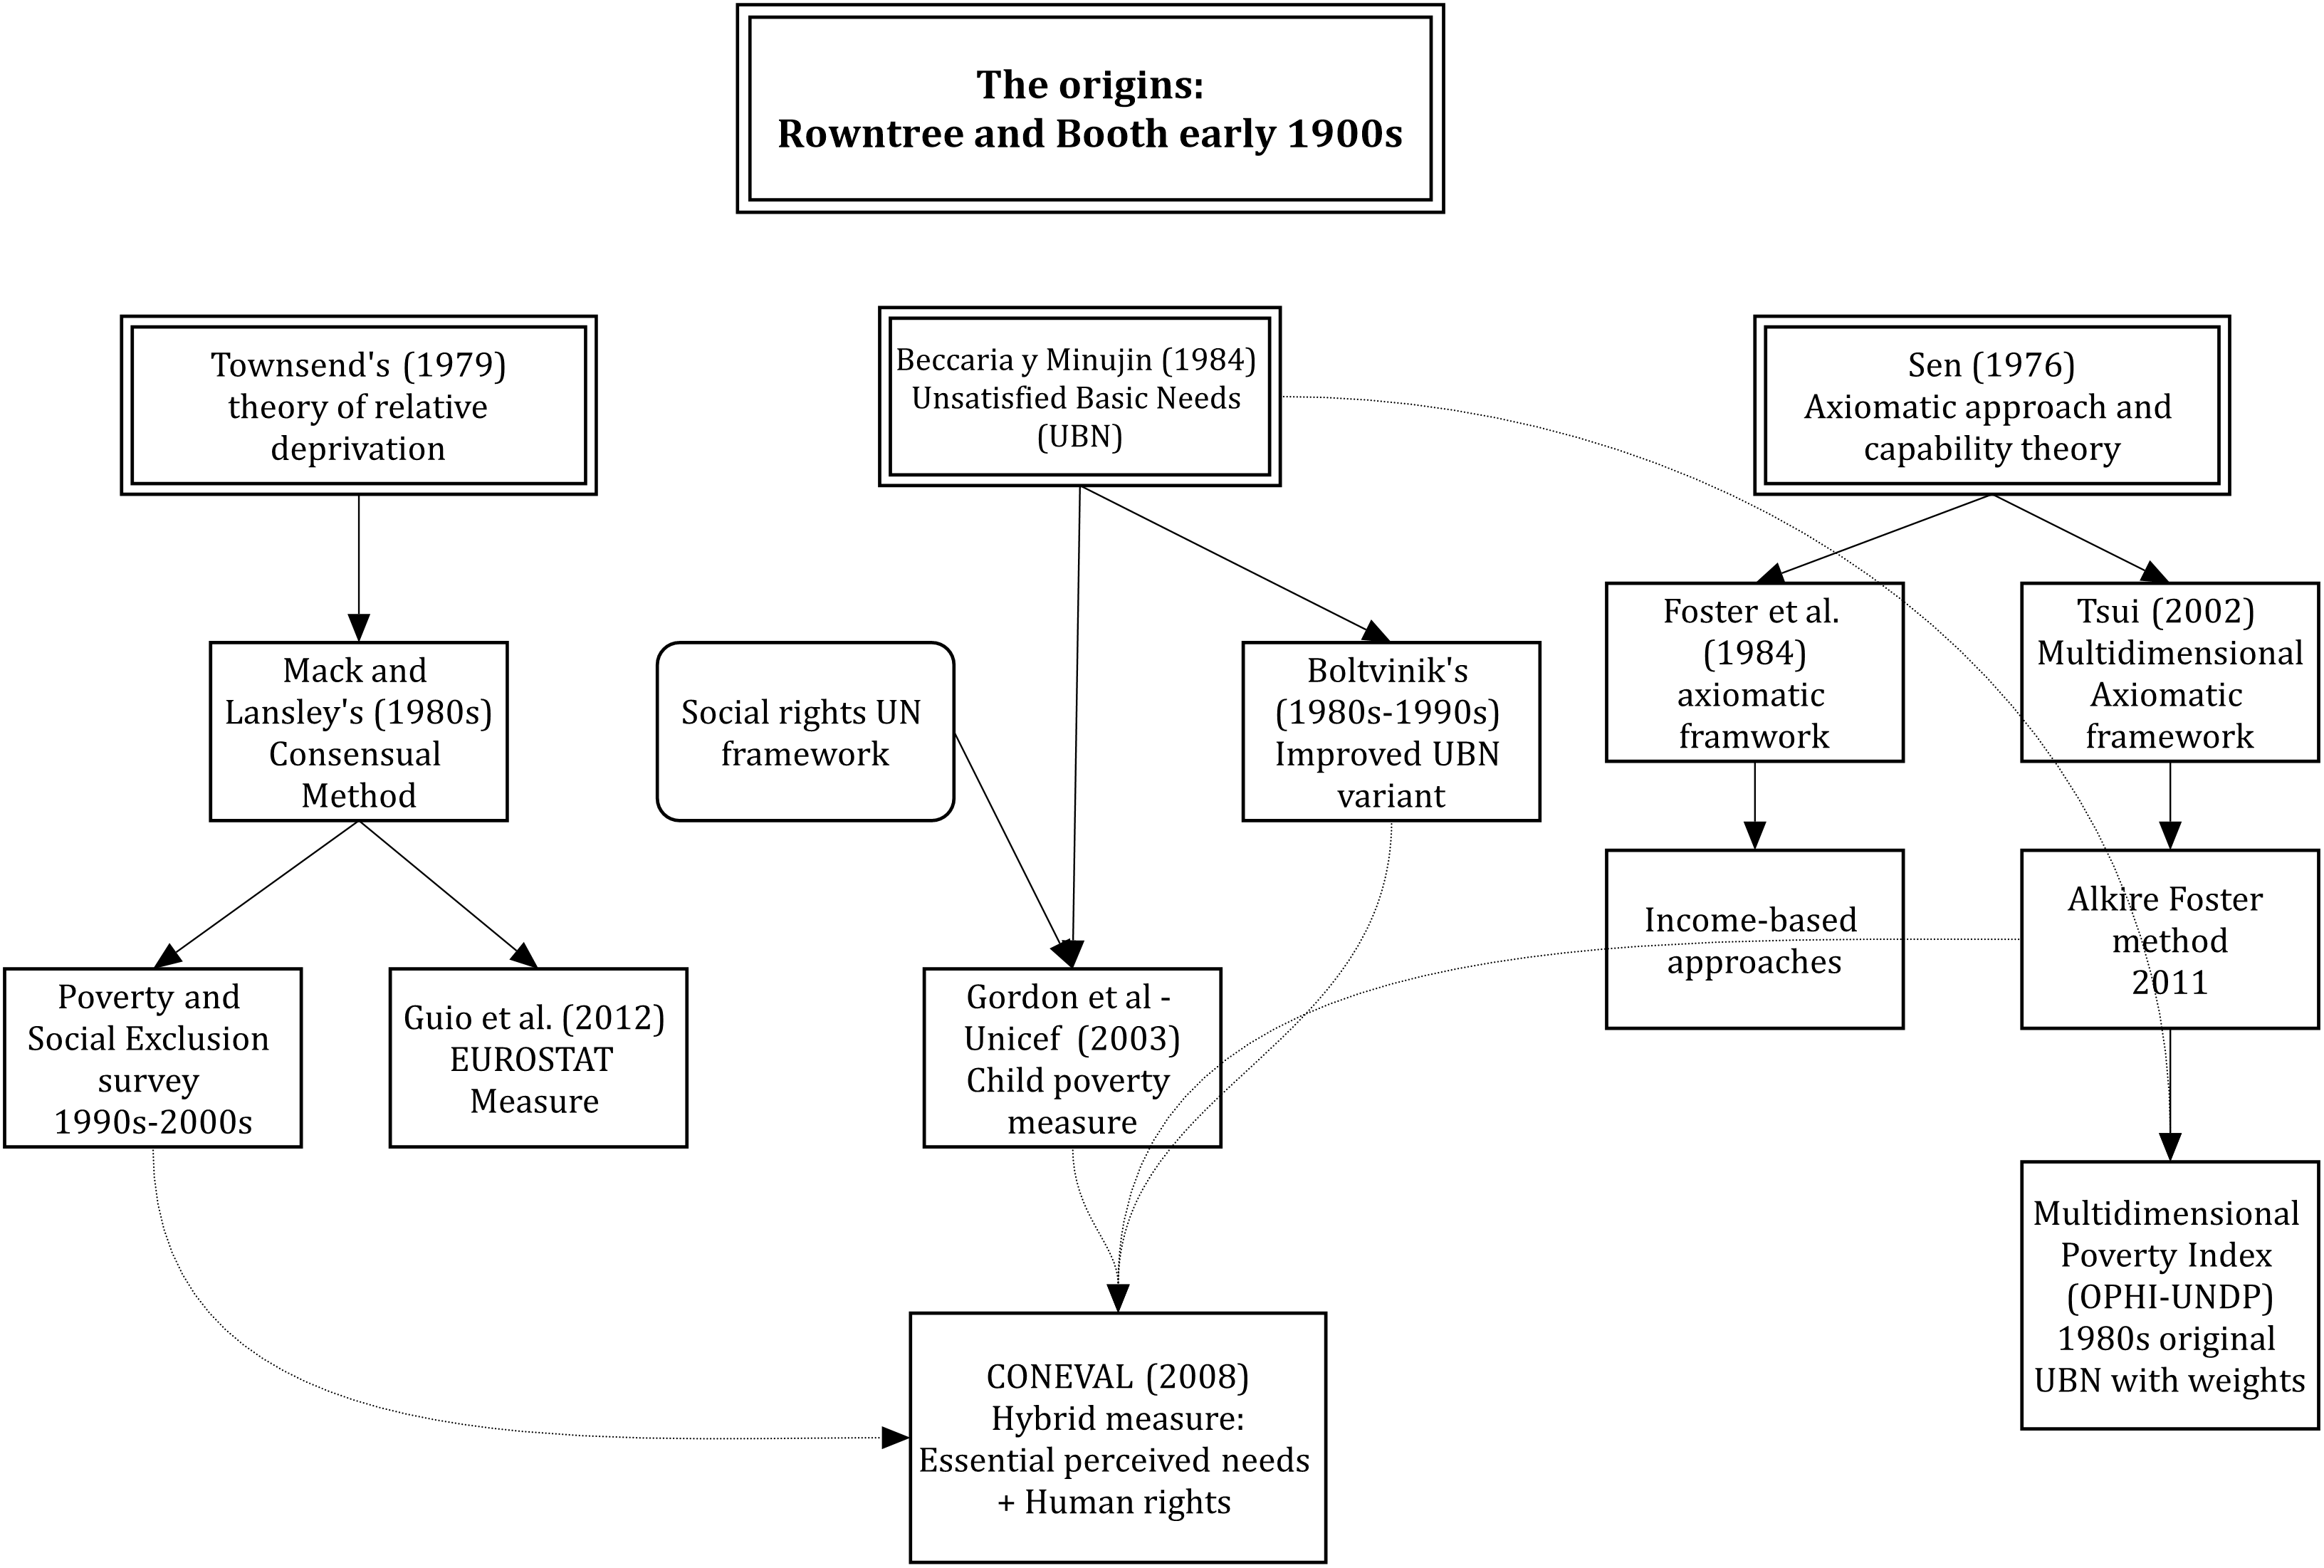
\includegraphics[width=\textwidth]{history_MPM} 

}

\caption{A brief summary of the history of poverty measurement}\label{fig:histMPM}
\end{figure}

The XXI Century was witnessed the resurgence of multidimensional measurement. In Europe the Poverty and Social Exclusion series has continued Townsend's tradition in the UK Townsend \& Gordon (\protect\hyperlink{ref-Townsend2000}{2000}), Pantazis, Gordon, \& Levitas (\protect\hyperlink{ref-Pantazis2006a}{2006}) and Mack \& Lansley (\protect\hyperlink{ref-Mack1985}{1985}) have had a major influence in the measurement of poverty in Europe (Atkinson, Guio, \& Marlier, \protect\hyperlink{ref-Atkinson2017}{2017}; Whelan et al., \protect\hyperlink{ref-Whelan2006a}{2006}). In economics, the axiomatic approach has been finally extended for multidimensional measures (Foster et al., \protect\hyperlink{ref-Foster2010a}{2010}; Tsui, \protect\hyperlink{ref-Tsui2002}{2002}). These contributions and the capability theory as overarching framework has been very influential in multidimensional poverty measurement (S. Alkire \& Foster, \protect\hyperlink{ref-Alkire2011a}{2011}; Alkire et al., \protect\hyperlink{ref-Alkire2015}{2015}; Kakwani \& Silber, \protect\hyperlink{ref-Kakwani2008a}{2008}). The efforts to articulate human rights and multidimensional poverty measurement have helped to the progressive institutionalisation either by nations or by international institutions of official multidimensional measures (Boltvinik, \protect\hyperlink{ref-Boltvinik2014}{2014}; CONEVAL, \protect\hyperlink{ref-CONEVAL2011a}{2011}\protect\hyperlink{ref-CONEVAL2011a}{a}). The work Gordon et al. (\protect\hyperlink{ref-Gordon2003}{2003}) on child poverty pioneered the era of global harmonized multidimensional poverty measurement by drawing upon human rights and UBN. The United Nations Development Programme (UNDP) global acute poverty measure in collaboration with the Oxford Poverty and Human Development Initiative (OPHI) that recovers some key dimensions of the UBN approach and aggregates the indicators using the AF methodology (Alkire \& Santos, \protect\hyperlink{ref-Alkire2010}{2010}; UNDP, \protect\hyperlink{ref-UNDP2014}{2014}). The most recent regional example is the EUROSTAT deprivation index that draws on relative deprivation and the consensual method (Guio et al., \protect\hyperlink{ref-Guio2017}{2017}, \protect\hyperlink{ref-Guio2016}{2016}).

Only two official measure have been put to statistical scrutiny: EUROSTAT and CONEVAL. The EUROSTAT measure was produced by Guio et al. (\protect\hyperlink{ref-Guio2012}{2012}) and revalidated by Guio et al. (\protect\hyperlink{ref-Guio2017}{2017}). It is based on the consensual approach and relative deprivation theory and has been fully statistically validated. The reason why there are several arrows pointing at the CONEVAL measure (the official Mexican measure) is that this is arguably the first official multidimensional measure and it had a desirable process for its production. After a critical change of the Social Development Law in 2004, Mexico was obliged to measure poverty from a multidimensional perspective and in accordance with the constitution. This resulted in an international consultation process. Mora (\protect\hyperlink{ref-Mora2010}{2010}) compiled the different contributions of the authors and CONEVAL (\protect\hyperlink{ref-CONEVAL2011d}{2011}\protect\hyperlink{ref-CONEVAL2011d}{b}) summarises the contributions of each author. The resulting measure is a hybrid measure that benefit from an international collaboration and it has been the first one to be fully statistically validated before its production. Townsend (\protect\hyperlink{ref-Townsend1979}{1979}) and the consensual approach were used to assess the thresholds for the nominal variables and provide a view on the socially perceived needs of the Mexican population with focus on social rights. Then Gordon (\protect\hyperlink{ref-Gordon2010}{2010}) conducted a preliminary evaluation of the indicators of the measure and suggested an approach to identify the poor and the not poor. Then the AF method was used to estimate the depth and intensity measures for income and the deprivation score.

Both EUROSTAT and CONEVAL have succeeded in producing measures that are not only theoretically sound but are also empirically validated. This is, nonetheless, an exception to the current practices in poverty research. The remainder of the book thus focuses on how to avoid producing magnifying-noise scales.

\hypertarget{poverty-and-measurement-theory-a-statistical-framework}{%
\chapter{Poverty and measurement theory: A statistical framework}\label{poverty-and-measurement-theory-a-statistical-framework}}

\textbf{Abstract}

This chapter outlines a statistical framework to tackle some of the challenges that involved in multidimensional poverty measurement. Measurement theory is posed as overarching framework for the assessment of some of the key assumptions made in the production of multidimensional poverty scales. The concepts of reliability, validity, measurement invariance and scaling are defined and put into the context of poverty research. Working examples of this concepts are then presented in the following chapters of the book.

\hypertarget{work-flow-in-poverty-measurement-a-falsifiable-framework}{%
\section{Work flow in poverty measurement: A falsifiable framework}\label{work-flow-in-poverty-measurement-a-falsifiable-framework}}

Chapter 1 outlined some of the tasks involved in the development of multidimensional poverty indices and highlighted the assumptions underlying each stage: dimensions, indicators and thresholds or cut-point selection; weighting of dimensions and indicators; aggregation or production of a score and setting of a poverty line Alkire (\protect\hyperlink{ref-Alkire2007}{2007}), Thorbecke (\protect\hyperlink{ref-Thorbecke2007}{2007}) and Gordon \& Nandy (\protect\hyperlink{ref-Gordon2012}{2012}).

Figure \ref{fig:realwf} illustrates the strategy often followed by researchers to produce a poverty index. Data often precedes the measurement (data ara given). Therefore, researchers have little influence upon the data collection process and thus they are constrained and have to adapt the existent information on deprivation to their poverty definition -or in the worst cases, they have to adapt the definition to the data-. A series of assumptions are raised with regard the number and type of dimensions, the indicators (including cut offs to identify deprivation) and weighting (see \protect\hyperlink{Chapter-1}{Chapter 1}. Ideally, these assumptions should be assessed using a framework but in practice researchers avoid this stage or they conduct a series of ad hoc sensitivity analyses. The limitation is that these kind of analyses have no hypothesis and researchers are more likely to confirm their beliefs due to the lack of a clear testable strategy. Confirmation biases, therefore, are more likely to remain and basically researchers jump from their theoretical measure to the aggregation procedure.

\begin{figure}[H]

{\centering 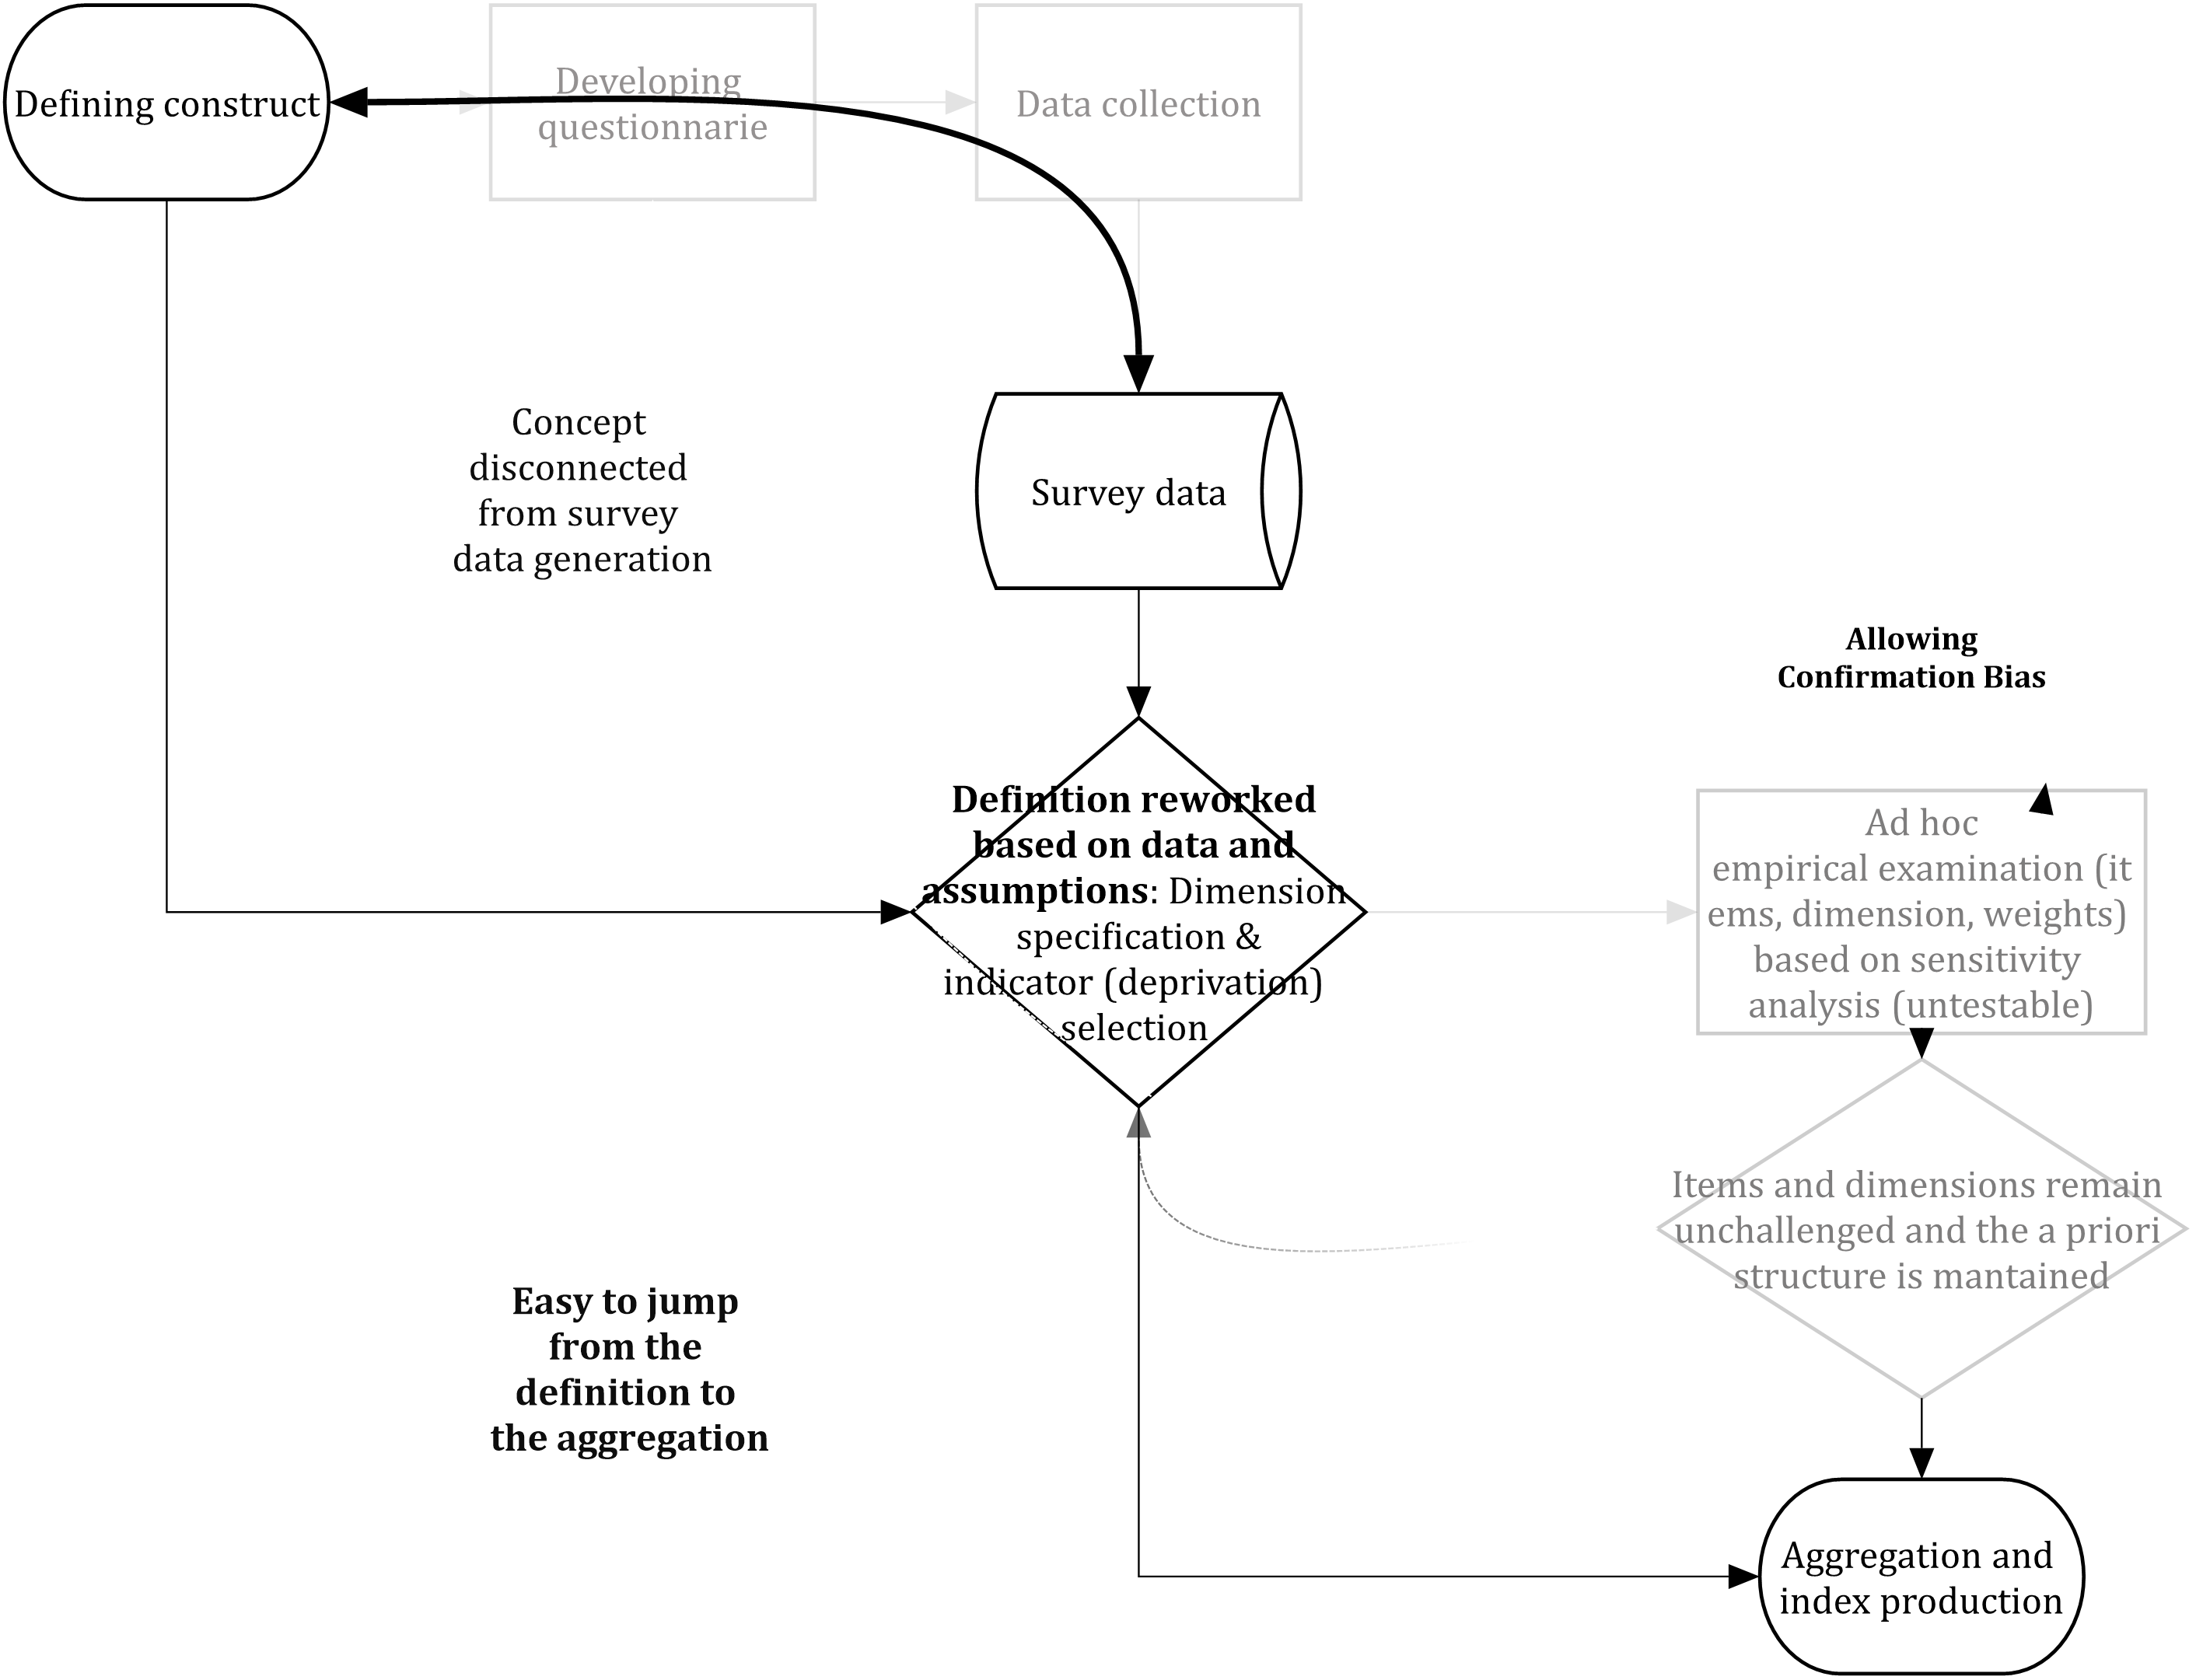
\includegraphics[width=\textwidth]{real_workflow} 

}

\caption{The work flow researchers often implement in multidimensional poverty measurement.}\label{fig:realwf}
\end{figure}

Scientific measurement aims to incorporate a framework to falsify researcher's assumptions. Figure \ref{fig:idealwf} shows the strategy that researchers could employ to reduce confirmation biases and measurement error. A theory of the concept of poverty should guide the development of a survey questionnaire and data collection. Researchers then could further especify the structure of their poverty measure based on the theory-driven data generation process. Once the theoretical measure is defined, assumptions need to be identified and make explicit so that can be falsified using a sound statistical framework. The results can be used as an input to redefine the measure in an iterative process. Once the measure is proven to be robust (using a definition of what a good measure is derived from a measurement framework), researchers could move onto aggregation and the identification of the poor and not poor groups.

\begin{figure}[H]

{\centering 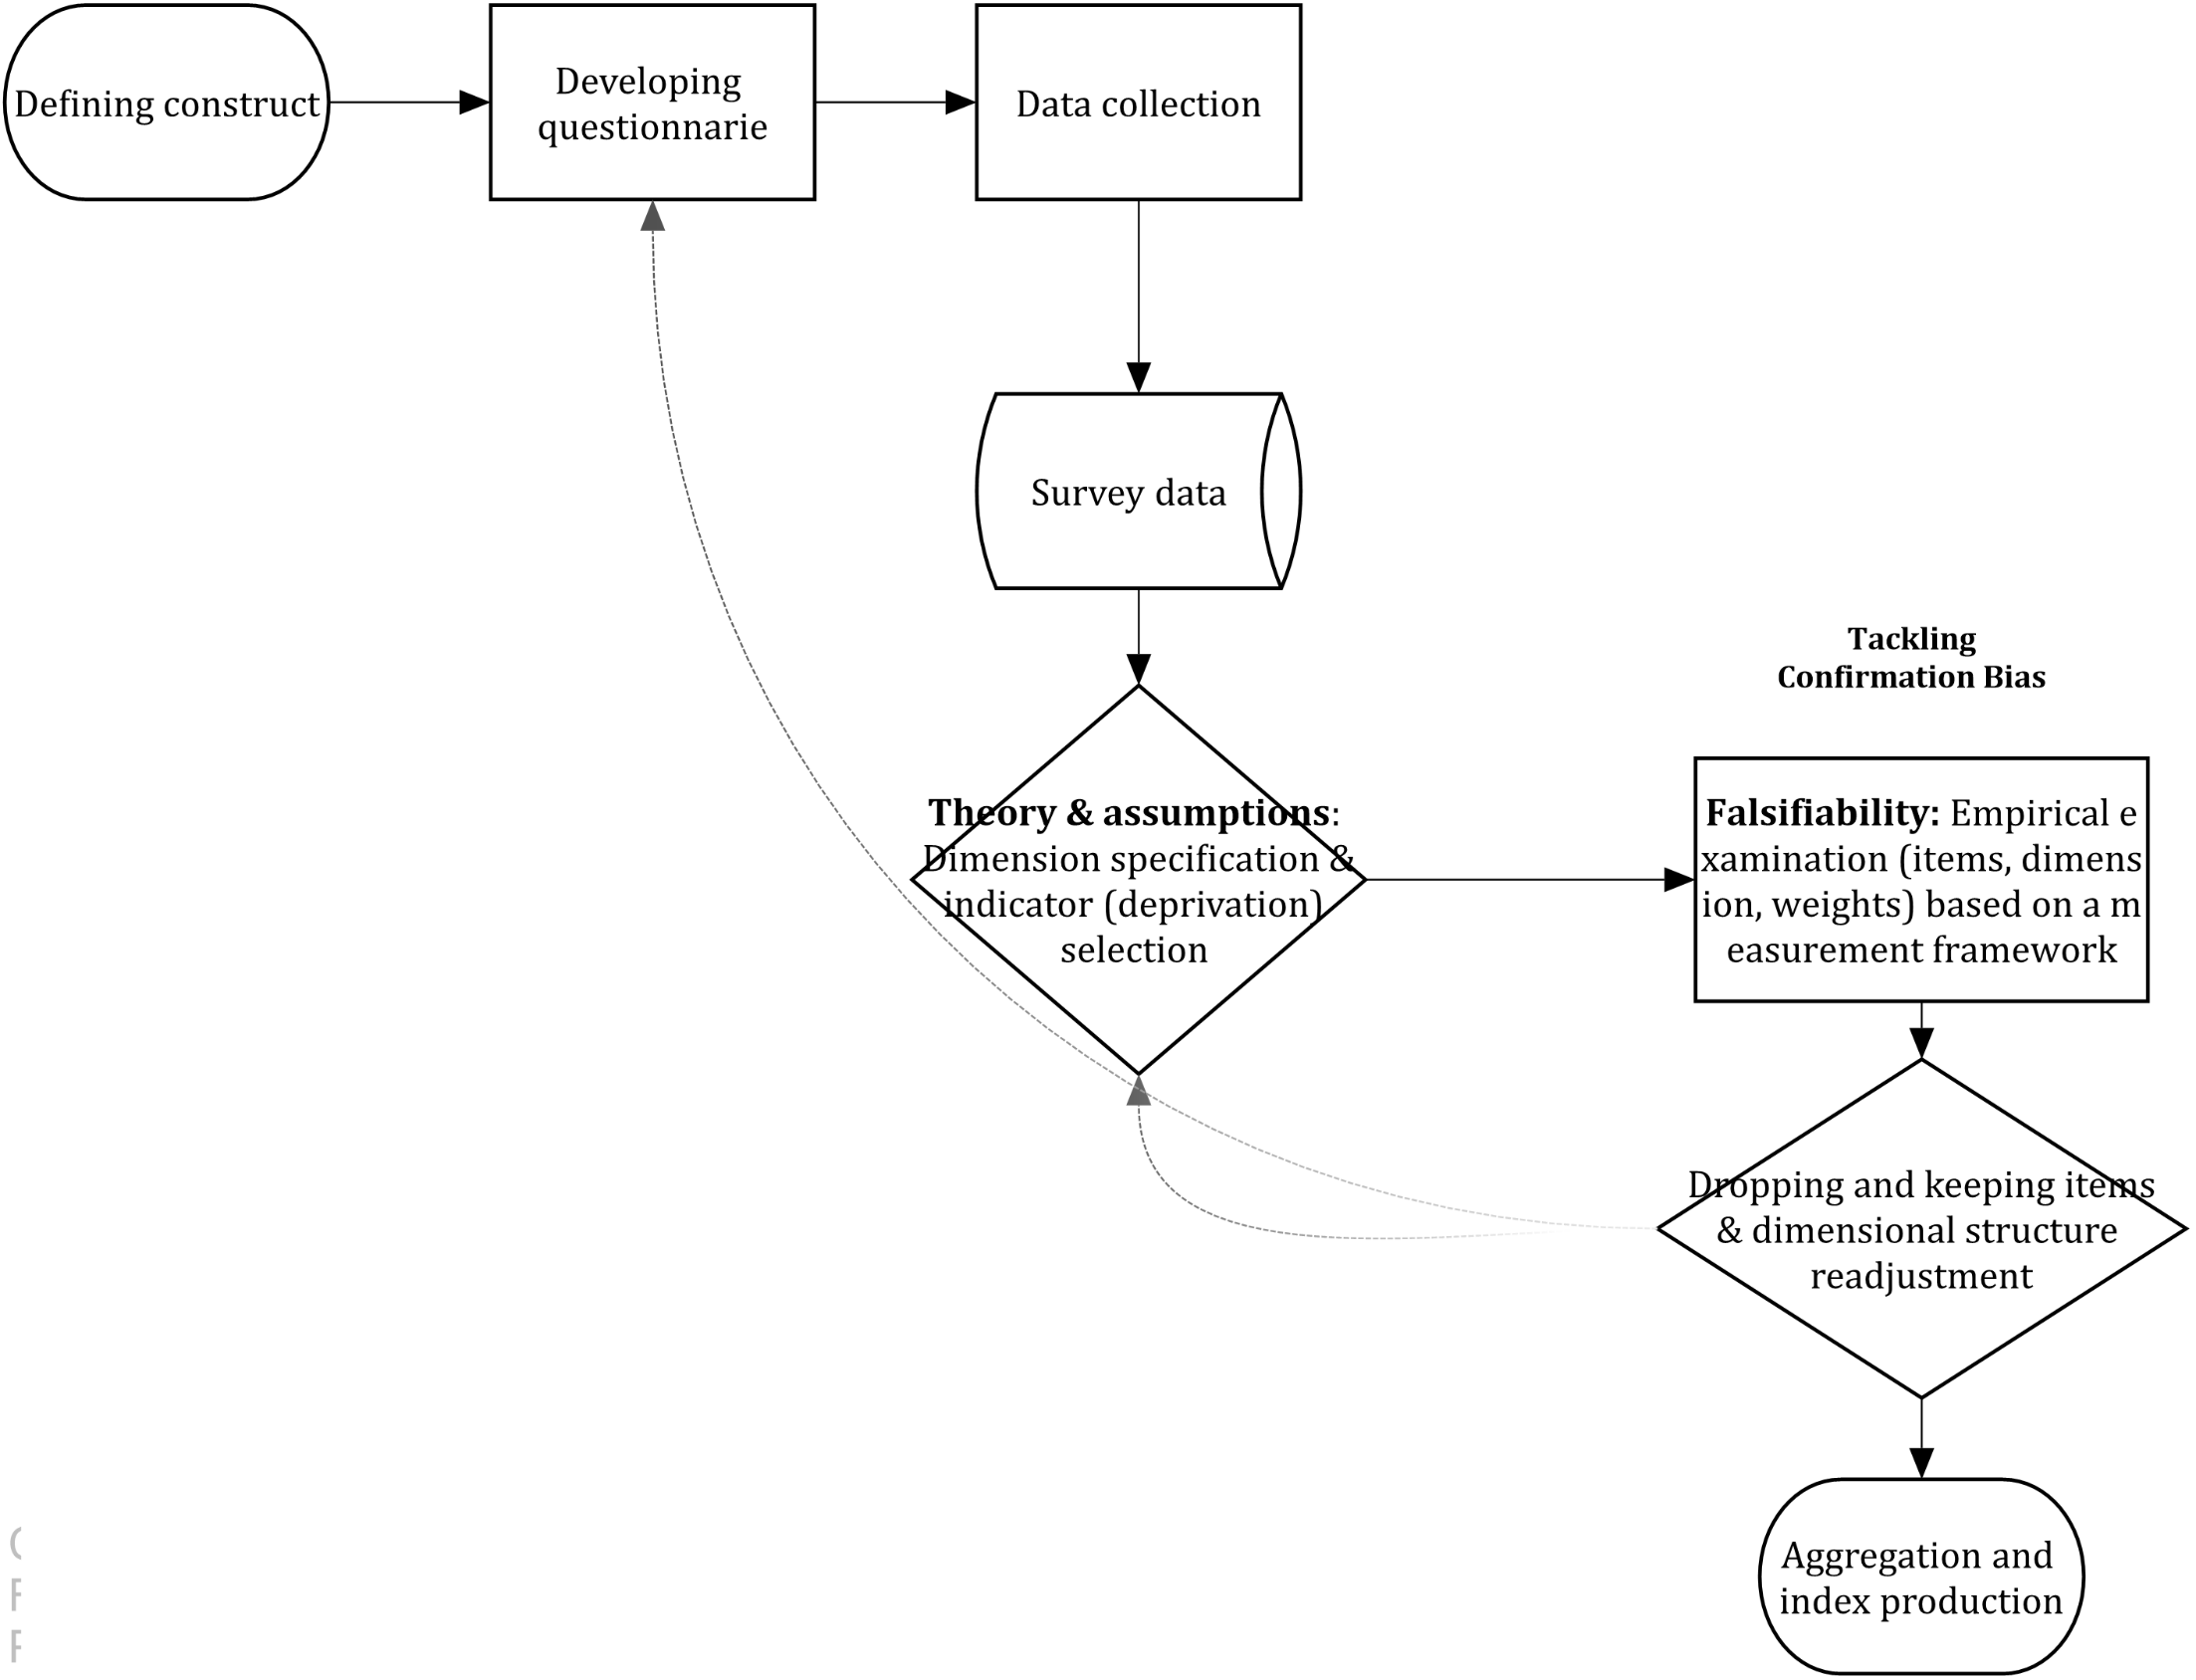
\includegraphics[width=3\textwidth]{ideal_workflow1} 

}

\caption{Ideal work flow in multidimensional poverty measurement.}\label{fig:idealwf}
\end{figure}

One possible and useful way to advance in the empirical assessment of poverty indices consist in detecting the assumptions involved in the production of an index and translate them into a falsifiable framework. That is, raising questions about all researcher's assumptions and propose a method to answer whether researcher's ideas hold given the data.

The challenges involved in poverty research can be put in terms of sequential stages following list of problematic or contested issues in poverty measurement. All these issues are part of an effort to approximate the extent and identification of poverty and can be therefore written in terms of a statistical model: a simplified and imperfect description based on observed data. As McCullagh (\protect\hyperlink{ref-McCullagh2002}{2002}) argues the idea of a statistical model conveys the recognition that the characterization of something is just an approximation. As such, a model to measure poverty is one possible option that can be assessed and improved. Before saying how a poverty measurement model can be examined and improved, is important to present an organised falsifiable framework of the key assumptions in poverty measurement.

\hypertarget{samplingspace}{%
\section{Identification of the sampling space}\label{samplingspace}}

One of the often overlooked features in poverty measurement is that fact that researchers never work with the full set of information. The main reason is that such set is unknown or unavailable. Given a definition of poverty, there are different dimensions, indicators and parameters to produce a working model to approximate poverty. But all these option belong to a space with all possible options. This is a major aspect of poverty measurement and highlights the fact that there is an underlying assumption (based on theory or data) about what subsets would work better to measure poverty.

\begin{enumerate}
\def\labelenumi{\arabic{enumi}.}
\tightlist
\item
  Sampling space of all possible dimensions \(\mathscr J\)
\item
  Sampling space of all possible variables \(\mathscr X\)
\item
  Sampling space of all possible parameters (e.g.~weights) \(\Theta\)
\end{enumerate}

This is just a statistical model throughout which poverty is identified and can compactly be written as:

\begin{equation}
\mathscr F = \{\mathscr X, F_{\theta} : \theta \in \Theta\}
\end{equation}

where the variables \(x_1,...,x_n\) follow a certain distribution \(F_{\theta}\), which is indexed by a parameter \(\theta\) defined in the parameter space \(\Theta\). \(\mathscr F\) is a family of all probability distributions on \(\mathscr X\), which is just the set of all possible observed data.

\hypertarget{selection-of-dimensions-and-indicators}{%
\section{Selection of dimensions and indicators}\label{selection-of-dimensions-and-indicators}}

Poverty measurement therefore involves sampling from different spaces (array of options). For example, they put forward some dimensions, variables and weights. This is often the first challenge in poverty measurement where researchers select some dimensions \(j\) from the sample space \(\mathscr J\) and some \(x_{ij}\) from the sample space \(\mathscr X\), so that if the scale has 30 indicators \(\mathscr X={1,2,...,30}\) where \(x_{ij}=1\) when deprived and \(x_{ij}=0\) (and \(z>0\) for binary variables). For nominal variables, there is a space of possible cut offs \(\mathscr Z\) too.

Selecting dimensions, indicators and thresholds involves making the assumption that the sampling from the different spaces is the best possible one, i.e.~the one that leads to a good poverty measure How does a researcher know whether its selection(sampling) is not wrong? This can be broken down into several questions:

\begin{itemize}
\tightlist
\item
  Is the subset of dimenions \(j\) from \(\mathscr J\) an \emph{adequate} characterization of poverty?
\item
  Is the subset of indicators given a cut off \((X;z)\) from \(\mathscr X\) an \emph{adequate} characterization of the dimension \(j\) and poverty?
\end{itemize}

The word \emph{adequate} is a loose term as this point as we need a theory or standard to define it. This is covered in the next section but at this point, the focus is on the into translating the challenges in poverty research into assumptions to build a statistical model (that later can be testable in some way).

\hypertarget{aggregation-and-weighting}{%
\section{Aggregation and weighting}\label{aggregation-and-weighting}}

The first stage is focuses in indicator and dimension selection and as it will be discussed below, this is where a falsifiable framework is more useful but also absent in poverty research. One way to illustrate it is with the AF method. The AF method will work fine as long as the components of the formula work fine but there is nothing within it that will ensure that this will be the case. Therefore, once the indicators have been selected, in a second state, researchers aggregate the variables using a linear model selecting some weights \(w \in \mathscr W\), where \(w_{ij}=1\) for non-differentially weighted measures and \(w_{ij}\ne 1\).

\begin{itemize}
\tightlist
\item
  Does the weighting scheme lead to the same ranking of the population?
\end{itemize}

\hypertarget{splitting-the-population-into-meaningful-groups}{%
\subsection{Splitting the population into meaningful groups}\label{splitting-the-population-into-meaningful-groups}}

Once the model of poverty has been completed \(\mathscr F\) a score is produced for each person in the sample. That means that a threshold should be proposed to identify the poor population.

\hypertarget{measurement-theory-as-an-statistical-framework}{%
\section{Measurement theory as an statistical framework}\label{measurement-theory-as-an-statistical-framework}}

\hypertarget{poverty-and-error-in-measurement}{%
\section{Poverty and error in measurement}\label{poverty-and-error-in-measurement}}

Poverty, as happens with many other constructs in social sciences, is an idea. It emerges from the theoretical presumption that within a population there is a group of people whose livings standard are below of what a society at a given point in time consider essential and customary to have a decent life. Poverty, in theory, impedes full participation in society, enhances the risk of die younger, interacts with many social risks, etc. But poverty is difficult to pinpoint because it is not directly observable and cannot be described with accuracy by a single variable. Instead, poverty research must rely on imperfect multivariate data to rank the population according to their living standards. To make things more difficult (see previous section), there are many ways in which poverty can be captured or described as researchers rely on different sets of outcomes (different samples from the same space) to characterise one's living standards (diverse deprivation/needs/achievements). Poverty thus is a latent variable in that several outcomes are utilized to imperfectly describe it\footnote{There is another framework that incorporates the idea of measurement error. Fuzzy sets theory uses the term vagueness to describe the intrinsic imperfection in poverty measurement (Martinetti, \protect\hyperlink{ref-Martinetti2006}{2006})}.

The problem of capturing poverty as a construct is just one of many cases in social sciences where researches face the difficulty of finding a theoretically constructed (unobservable) group (e.g.~the depressed, high class, high-achievers in education, happy). How then can we detect a group of people belonging to a construct? Spearman (\protect\hyperlink{ref-Spearman1904}{1904}) put forward a capital idea: two or more outcomes is an indication that two things may have the same underlying cause. This perfectly fits the theory that deprivations are an observed outcome of poverty. A core assumption in poverty measurement is that a set (\(X \in \mathscr X\)) of indicators constitutes the series of relevant manifestations of the idea of poverty. This treatment of poverty as a construct is powerful in that is a theoretical underpinning and rationale for finding and ranking individual differences in living standards (below which one is poor).

Deprivation indicators are intercorrelated because they share a common cause: poverty. Conceptually, this means that if the effect of poverty is eliminated the inter-correlation of outcome variables would be zero. Measurement theory postulates that the problem of the relevant set of outcome variables to measure poverty can be tackled from the perspective of the \emph{common factor model} Thurstone (\protect\hyperlink{ref-Thurstone1947}{1947}). Such a model formally postulates that the observed outcome is a function of one or more common factors and one unique factor. Each deprivation should vary due to two main sources (1) common variance and (2) unique variance. The first type of variance is the one accounted by for the latent factor- the variance shared with the other outcome measures. The second is the variance accounted by for other factors and by random error (unreliability, measurement error).

\hypertarget{measurement-model-for-poverty}{%
\section{Measurement model for poverty}\label{measurement-model-for-poverty}}

The statistical model proposed in modern measurement theory would be a common factor model where each observed variable (\(x_{ij}\)) is a product of a latent dimension (\(\eta_j\)) and the higher order factor (\(\zeta_h\)) overall poverty. One of the interesting aspects of this formulation is that
as not everything is due to the latent variable, error theory of a measurement model includes the method effect.

\begin{equation}
\label{eq:model1}
 x_{ij} = \lambda_{ij} \eta_j + \varepsilon_ij  
\end{equation}

\begin{equation}
\label{eq:model2}
 \eta_j = \gamma_{j} \zeta  + \xi 
\end{equation}

The \(\lambda_{ij}\) and \(\gamma_{j}\) are known as factor loadings and they capture the relationship between the latent variables and the outcome measures, and between the dimensions and the overall latent variable. Of course, it is possible to have more \(\zeta\)'s but in poverty research the presumption seems to be that dimensions are nested into one overall latent construct which is poverty (some especial cases will be shown in Section XX where the higher-order model is a third-order factor):

Poverty → Dimensions → Sub-dimensions → outcome measures.

This model specification is one way to statistically capture the way in which multidimensional poverty measurement is conducted in the contemporary literature. Researchers propose a series of dimensions and classify their proposed indicators accordingly. The crucial aspect is that this is just an idea -informed from some theory or data- about how poverty can be better captured under a multidimensional definition. That is, the proposal is just an invalidated model that demands scrutiny. When put in terms of equation \eqref{eq:model1} and equation \eqref{eq:model2} researchers move from theoretical speculation toward empirical falsification.

\hypertarget{blueprints-and-poverty-measurement-models}{%
\section{Blueprints and poverty measurement models}\label{blueprints-and-poverty-measurement-models}}

Models are just blueprints that summarise an explanation of how things can be constructed. Putting theoretical proposals to measure poverty in terms of a diagram helps a lot to visualise and contrast the diverse proposals to measure poverty. The advantage of measurement theory is that everything can be put in terms of a blueprint. Multidimensional models can be easily presented as a diagram, which is just a graphical representation of a model. Another way to think about this, is to see the different blueprints in poverty measurement are just the different ways in which researcher sample from \(\mathscr J\) and \(\mathscr X\). They lead to diverse structures, i.e.~models.

Equation \eqref{eq:model1} simply tells a model in which one latent construct produces the observed (\(x_{ij}\)) outcomes. This model is say to be unidimensional as there is only one factor \(\eta_j\) causing the observed indicators. One could think of this model as the null model in poverty measurement where the indicators cannot be clearly clustered into dimensions. This does not mean that the indicators do not measure different aspects of poverty. It might be that the indicators indeed different aspects but that there are no clusters of indicators. In practice, there are few theoretical models proposing such thing. Empirically, however, it might be often a case given that in poverty research data collection rarely follows a theoretical proposal (see \emph{add chapter reference}). Figure \ref{fig:cfanull} translates \eqref{eq:model1} into a plot.

\begin{figure}

{\centering 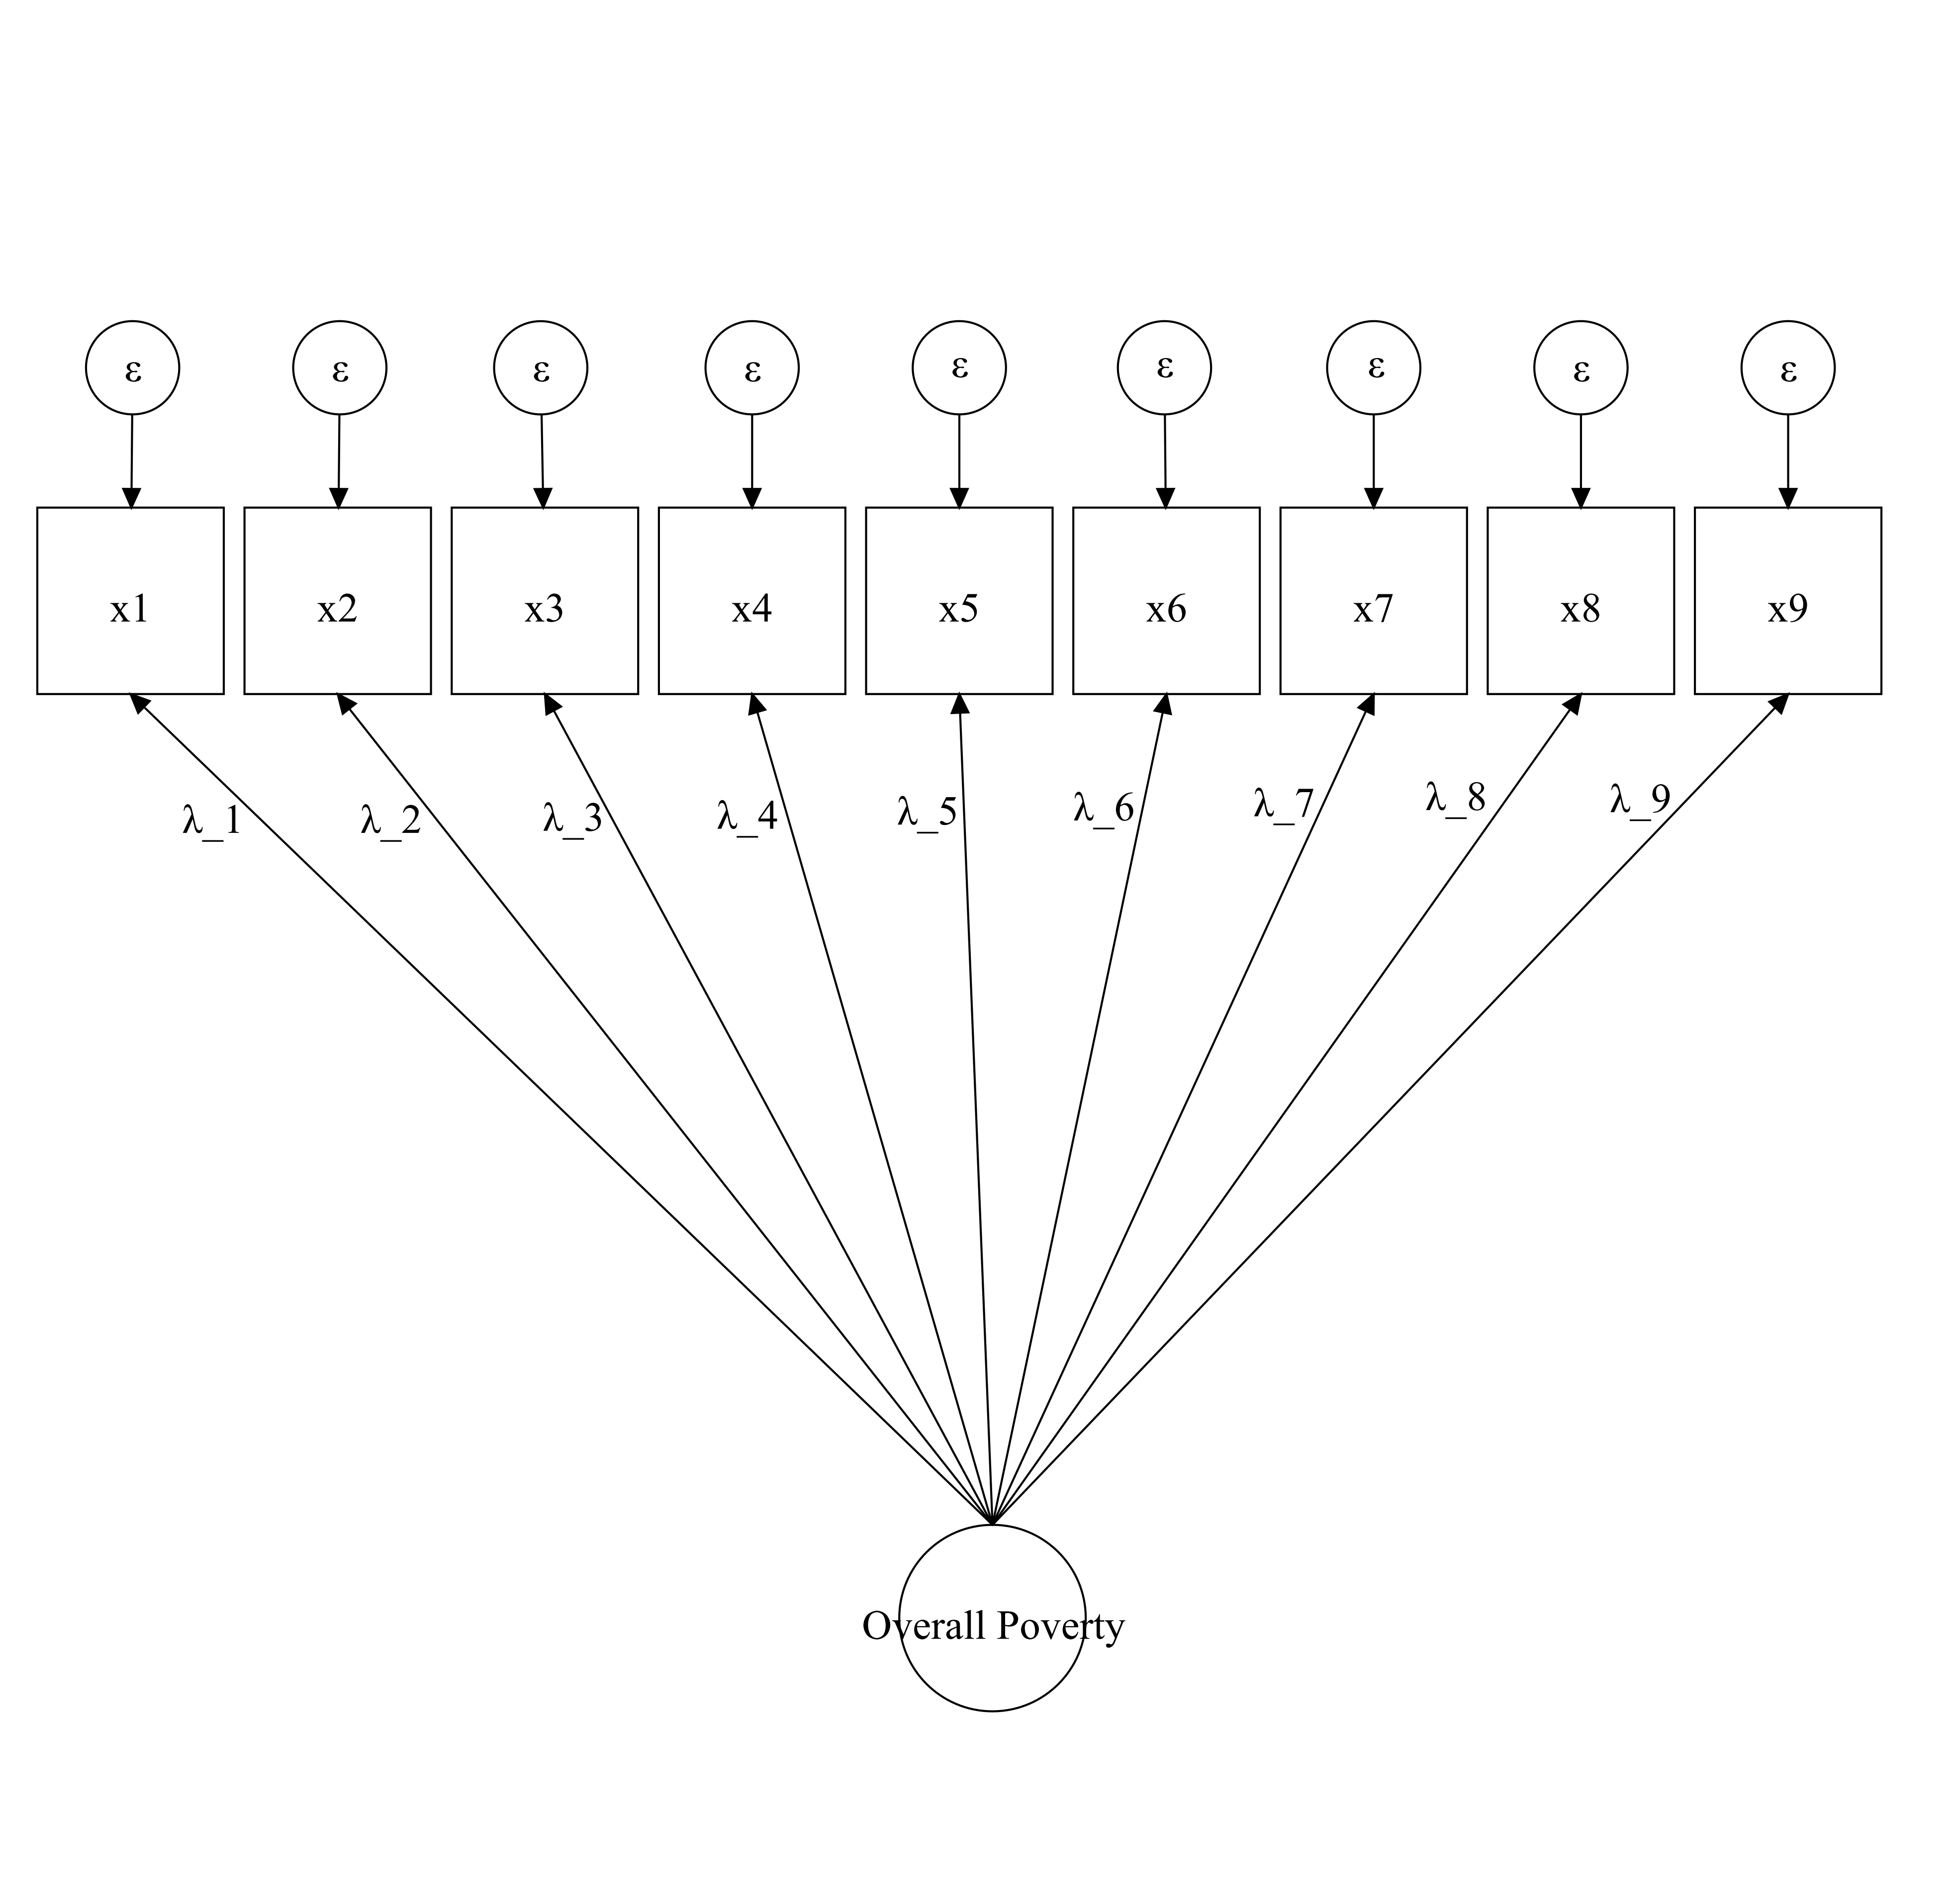
\includegraphics[width=\textwidth]{Diagram_CFA_null} 

}

\caption{This is a visual representation of a null unidimensional model.}\label{fig:cfanull}
\end{figure}

Figure \ref{fig:cfaguio} displays the higher order factor model using the three dimensions proposed by A Guio et al. (\protect\hyperlink{ref-Guio2009}{2009}). This structure is roughly what poverty researchers have in mind when thinking about poverty in multidimensional terms. That is, that the indicators can be grouped into some dimensions. In this example, there are 9 outcome variables classified into three dimensions (\(\eta_j\)) (Durables, Housing and Economic strain). Then the loadings (\(\lambda_{ij}\)) denote the relationship of each outcome with the dimensions in question. Then the arrows from the high-order factor (overall poverty) to each dimension are the factor loadings (\(\gamma_{j}\)) that capture the relationship between overall poverty and each dimension. Both (\(\lambda_{ij}\)) and (\(\gamma_{j}\)) are parameters of the model and denote the strength of the association between the latent variable and the outcome variables (See \emph{\ref{cha:reliability}} for an explanation of how this relates to the topic of reliability and differential weights). The diagram of @(fig:cfaguio) model is an example of a higher-order factor: A three-dimension model with a higher-order factor. The dimensions are durables, housing and economic strain. In this example, there are only three indicators for each dimension. In this model, none of the indicators loads into more than one dimension. Poverty measures often assume that a given indicator is an exclusive outcome of a certain dimension.

\begin{figure}[H]

{\centering 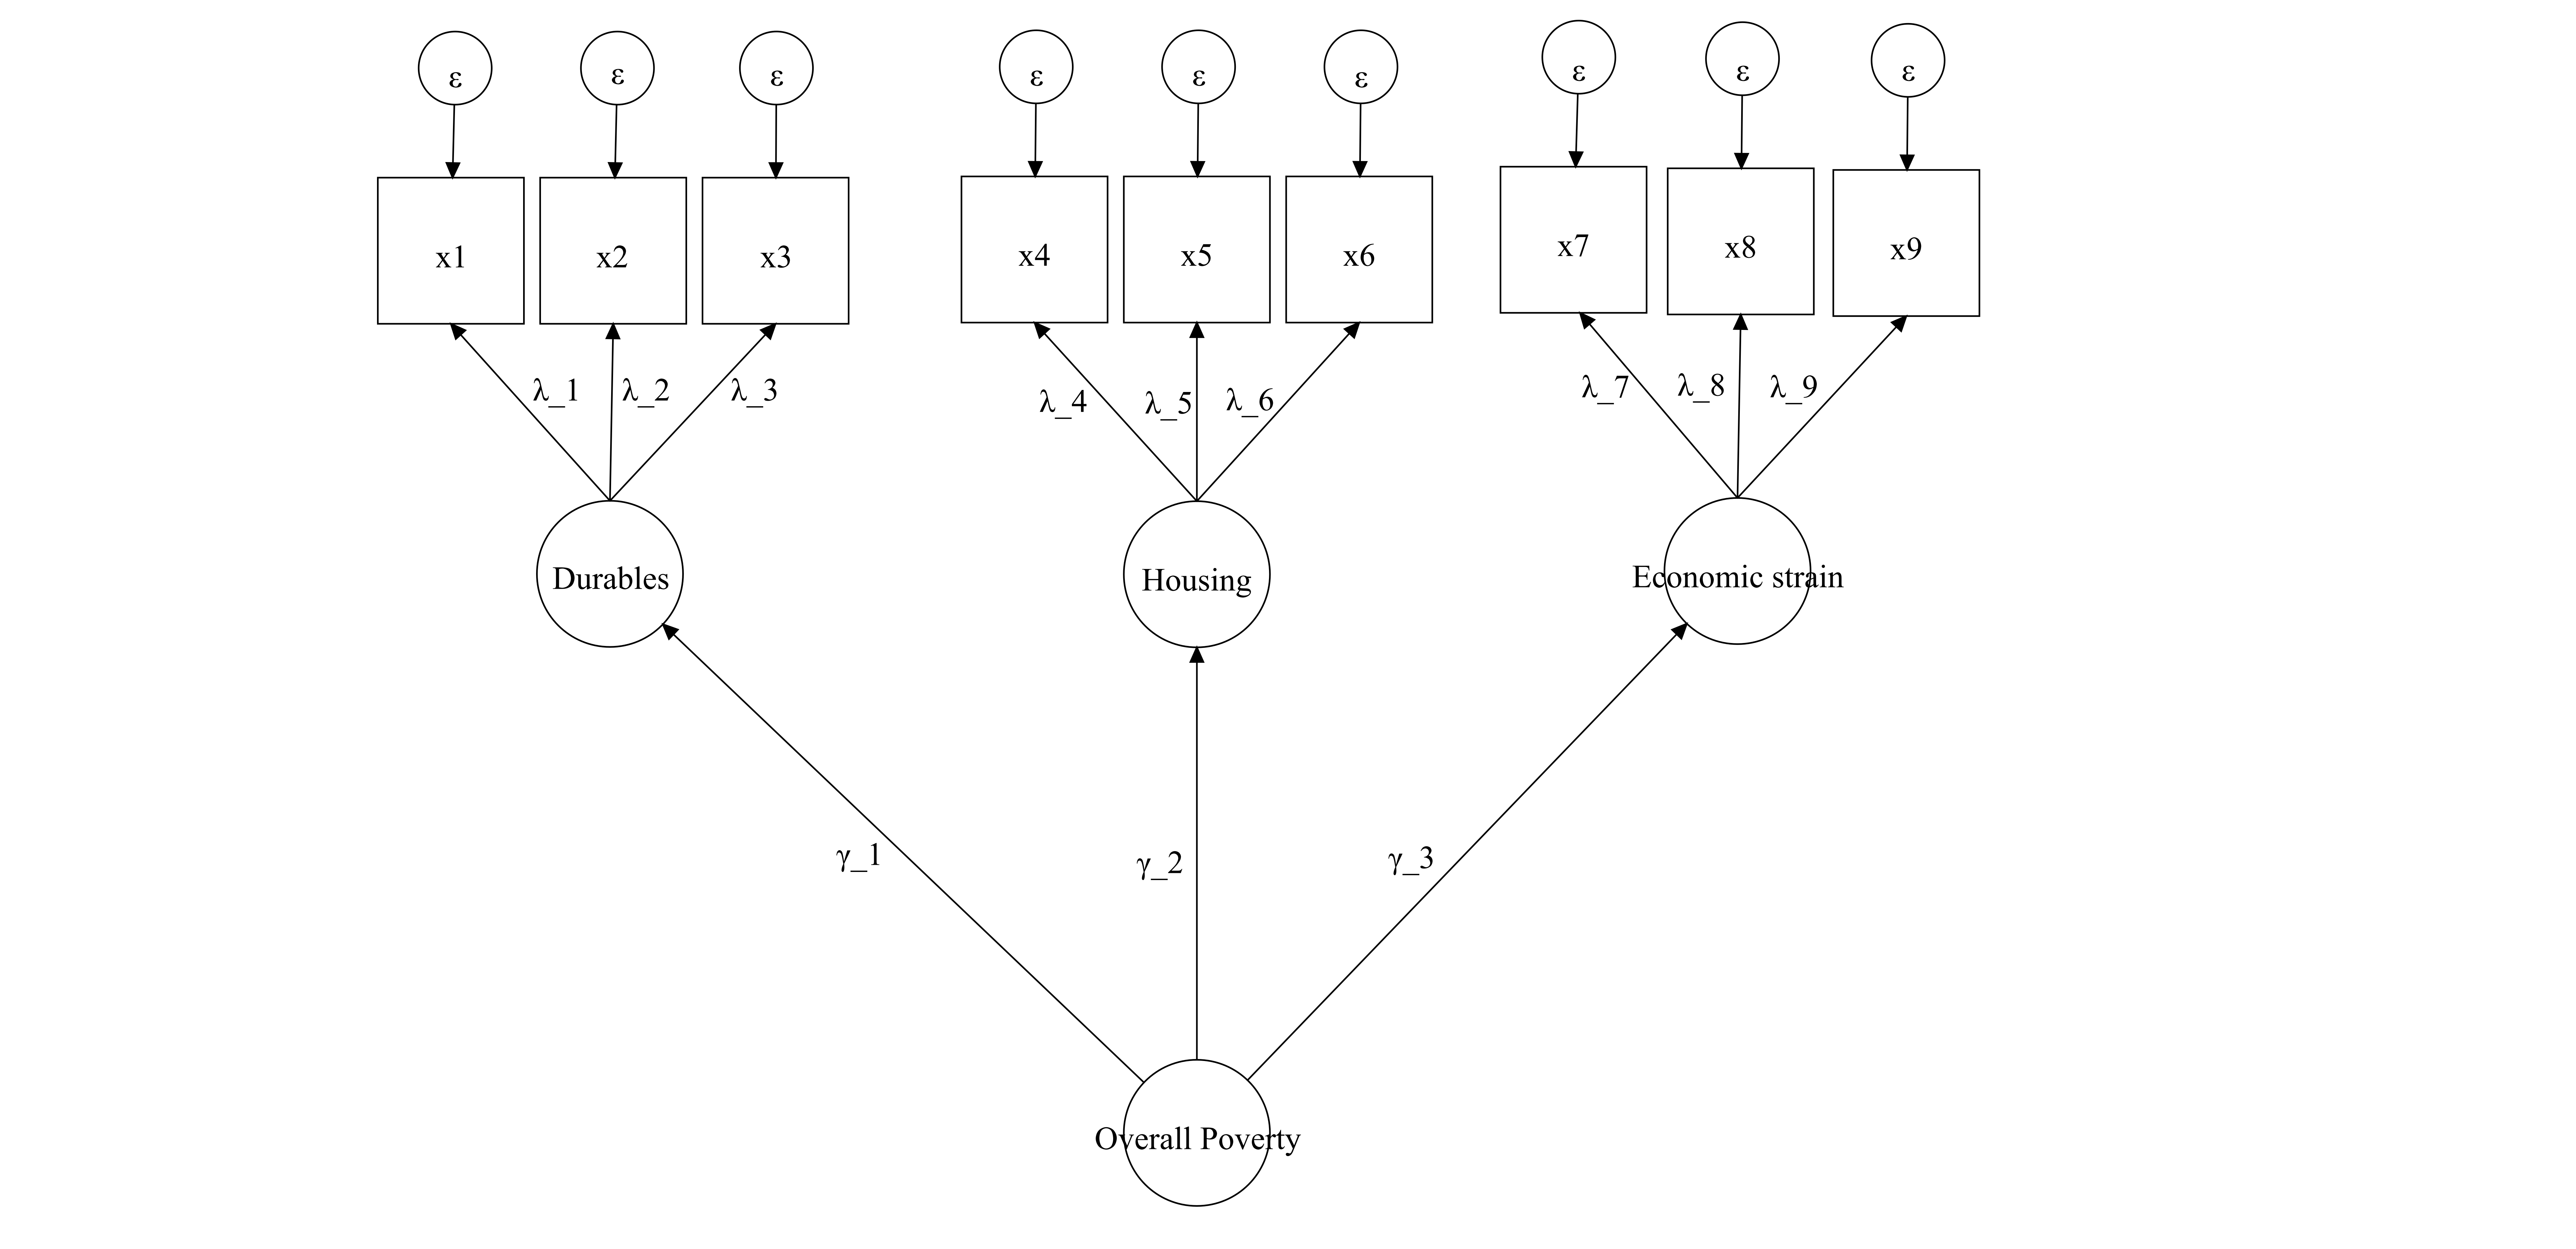
\includegraphics[width=\textwidth]{Diagram_CFA_GuioModel} 

}

\caption{This is a visual representation of @Guio2009's model. Second-order factor.}\label{fig:cfaguio}
\end{figure}

Another way to think about the dimensions of poverty comes from Alkire \& Santos (\protect\hyperlink{ref-Alkire2010}{2010}), which is used to compute OPHI-UNDP's Multidimensional Poverty Index (MPI). The structure proposes a similar structure to Guio et al. (\protect\hyperlink{ref-Guio2009}{2009})'s model: second-order structure. In this case, poverty is thought to have three substantive dimensions: Education, health and iving standards. These are different dimensions from those porposed by Guio et al. (\protect\hyperlink{ref-Guio2009}{2009}) or by Townsend (\protect\hyperlink{ref-Townsend1979}{1979}) in figure \ref{fig:cfampi}. The diagram only specifies, at this point, the structure of the measure as the MPI does not have three indicators for each dimension but it helps to see the model the authors put forward to measure global acute poverty.

\begin{figure}[H]

{\centering 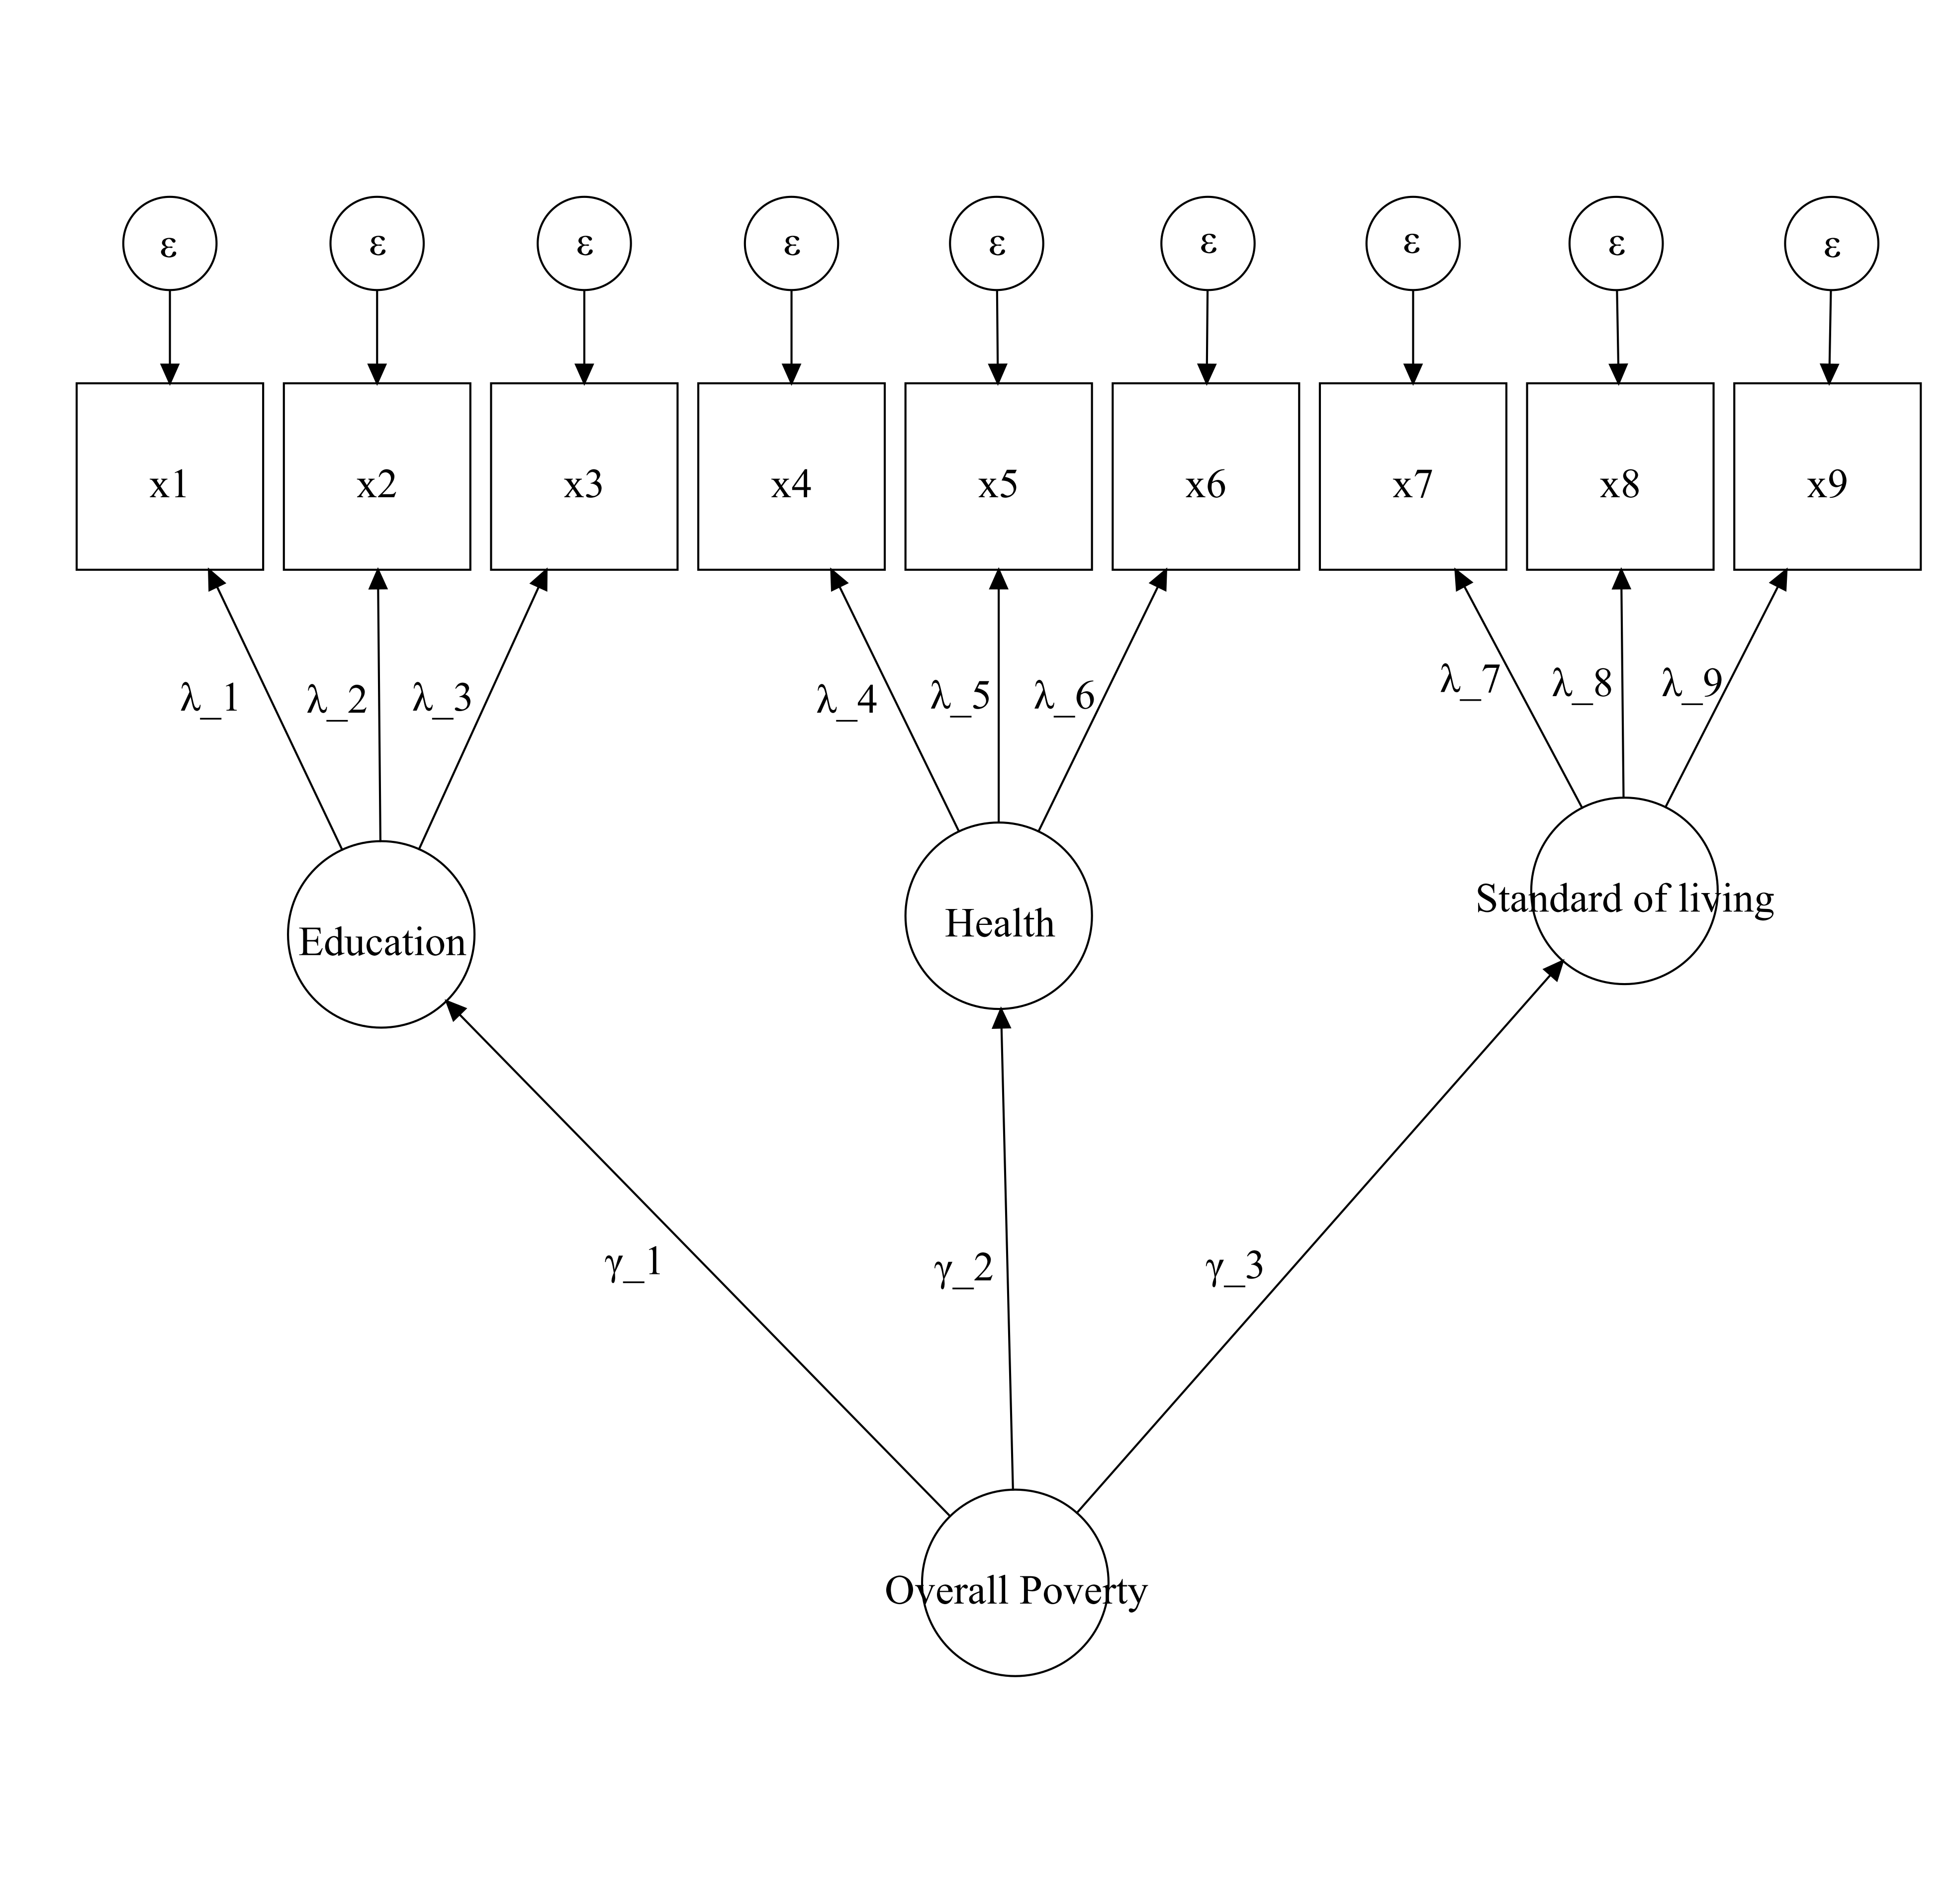
\includegraphics[width=\textwidth]{Diagram_CFA_mpi} 

}

\caption{This is a visual representation of @Alkire2010's model. Second-order factor}\label{fig:cfampi}
\end{figure}

Townsend (\protect\hyperlink{ref-Townsend1979}{1979})'s model is one of the first multidimensional models in the world. His proposal has more nested dimensions compared with figures \ref{fig:cfaguio} and \ref{fig:cfampi}. In this case, indicators are nested into eleven dimensions, which in turn can be grouped into two more dimensions. The resulting figure (\ref{fig:cfatownsend} is a third-order factor structure. Guio et al. (\protect\hyperlink{ref-Guio2017}{2017}) propose a reduced version of this model which does not considers the 11 dimensions and indicators are classified according to material and social deprivation. The loadings of the indicators are ommited. \(\kappa_1\) and \(\kappa_2\) are the loadings of the higher order factor. These could be specified using \eqref{eq:model2} as reference- now \(\zeta\) has k=2 factors.

\begin{figure}[H]

{\centering 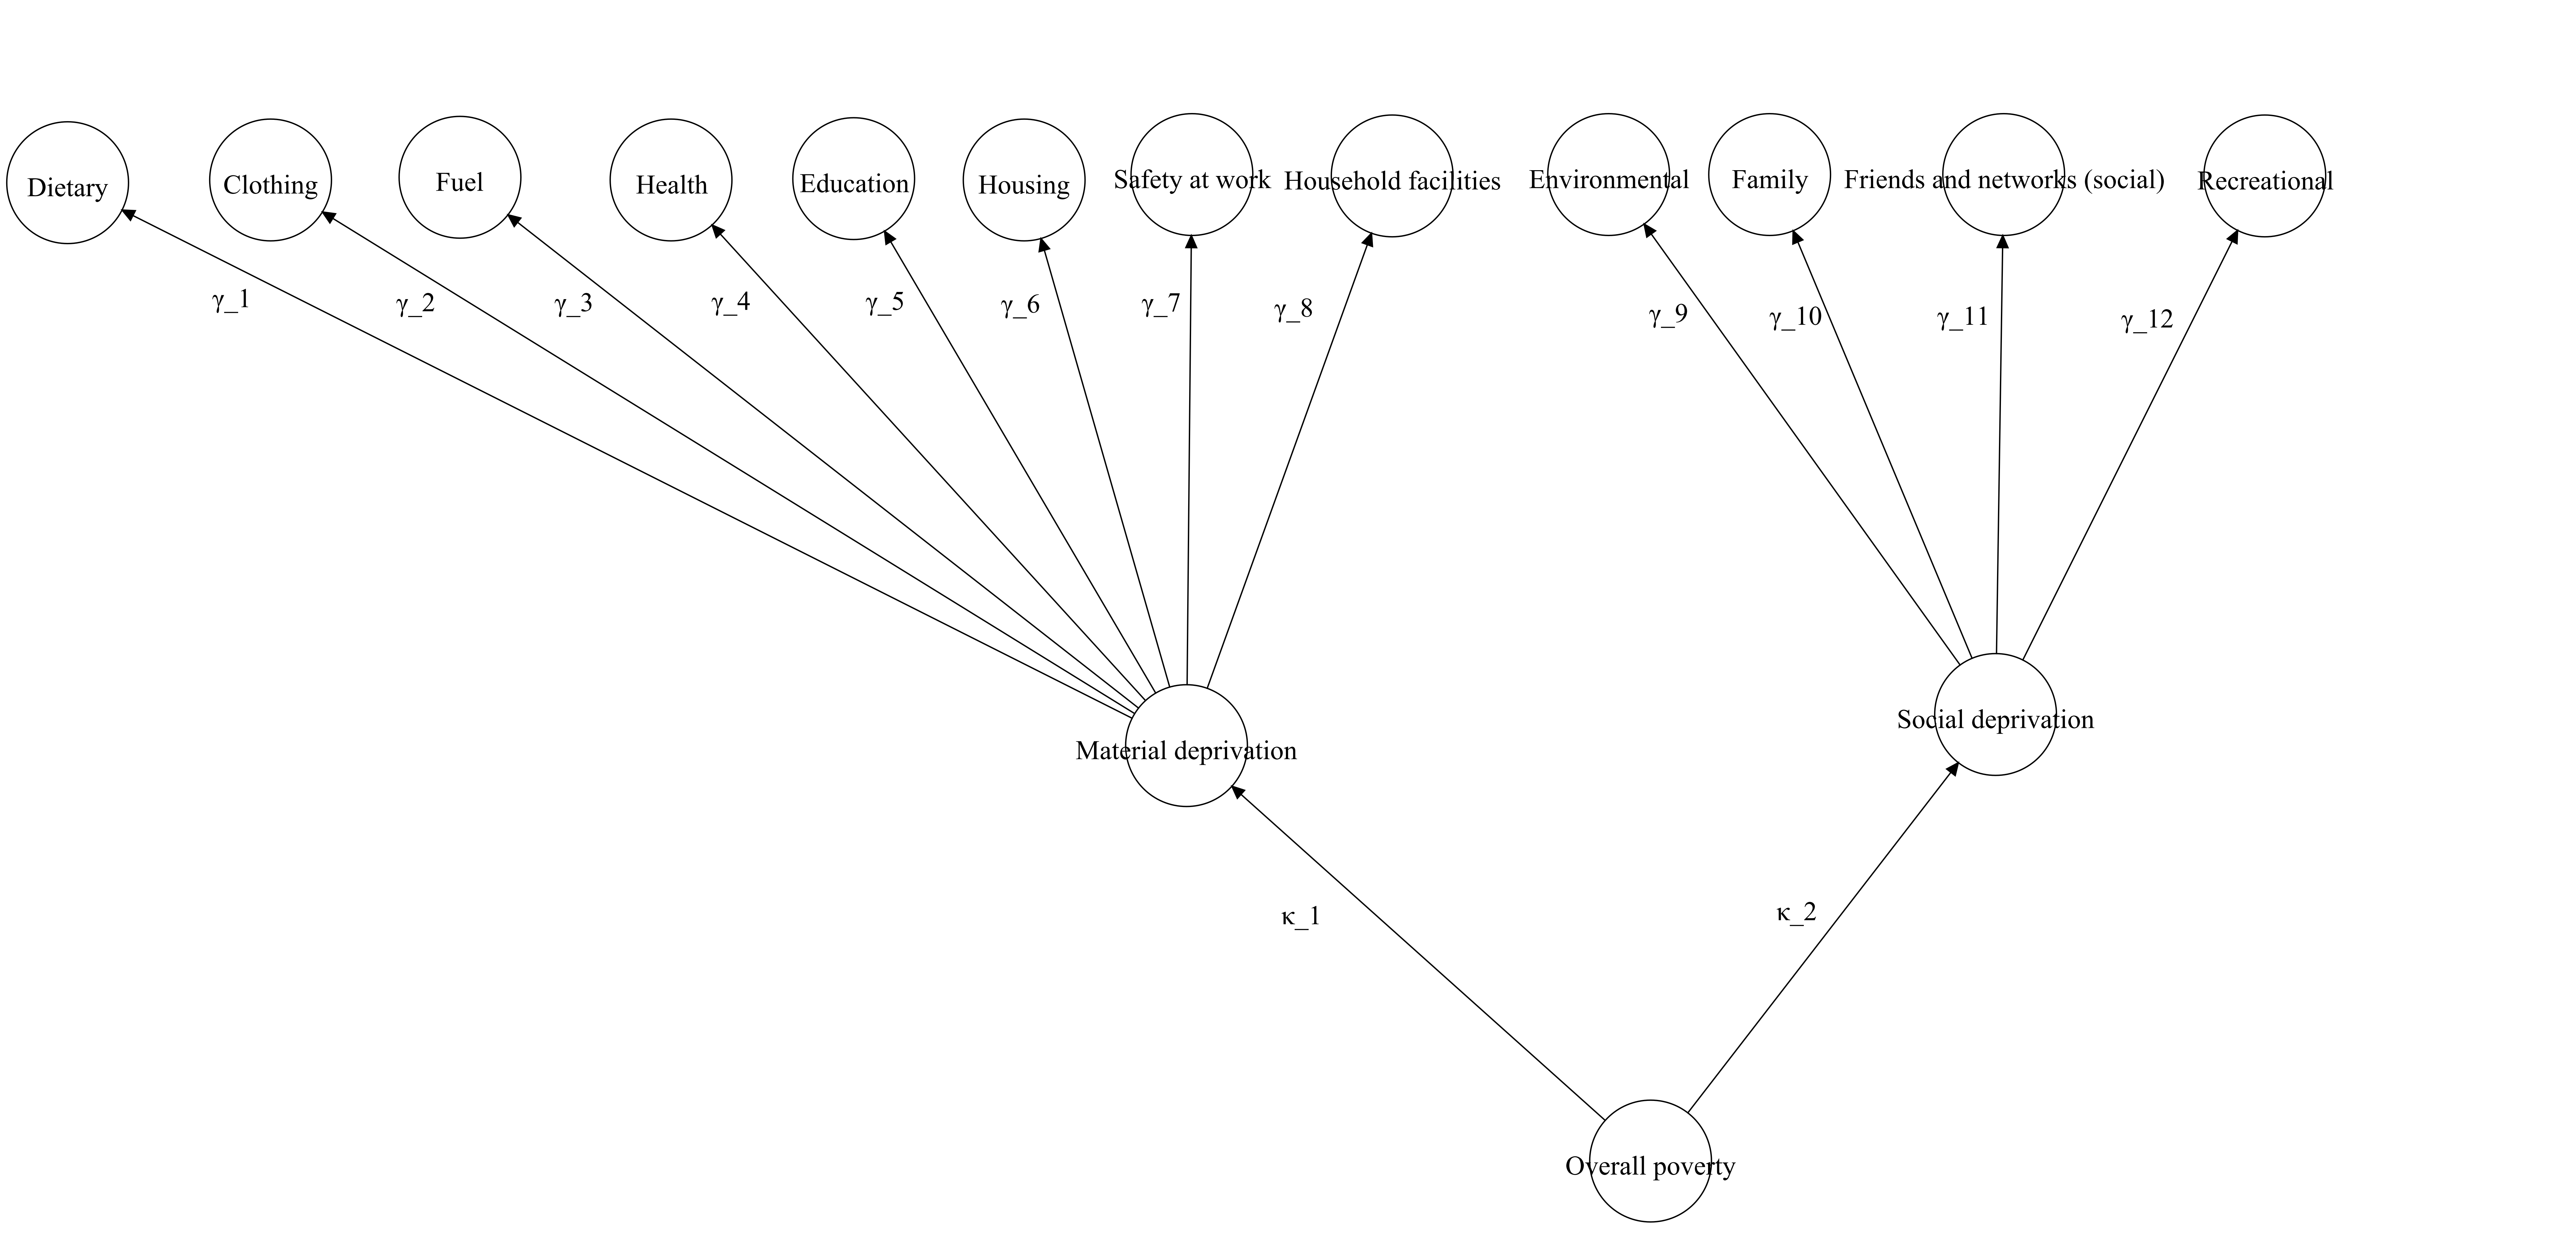
\includegraphics[width=\textwidth]{Diagram_CFA_townsend} 

}

\caption{This is a visual representation of @Townsend1979's model. Third-order factor.}\label{fig:cfatownsend}
\end{figure}

Another way to think about this, is to see the different blueprints in poverty measurement are just the different ways in which researcher sample from \(\mathscr J\) and \(\mathscr X\). They lead to diverse structures, i.e.~models. This reflection brings us back again to the question: how do we know whether the samples we take from \(\mathscr J\) and \(\mathscr X\) are an adequate representation of poverty in a given society at a given point in time?

\hypertarget{measurement-theory-and-principles}{%
\section{Measurement theory and principles}\label{measurement-theory-and-principles}}

One central debate in poverty measurement is about the dimensions of poverty. The discussion revolves around questions such as: How many dimensions are? What are the contents (indicators) of these dimensions? How dimensions are associated and differentiated? Does these dimensions have equal importance? (see \emph{\ref{cha:Chapter_1}}). The previous section translated these questions into concrete challenges and advanced a general framework of measurement that explicitly acknowledges that all measurement practices involve different kinds of error. However, the framework is incomplete. It requires some governing principles that effectively put the work flow in poverty measurement in terms of a cogent falsifiable framework. One crucial question raised in section\textasciitilde{}\emph{\ref{sec:samplingspace}} are:

\begin{itemize}
\tightlist
\item
  Is the subset of dimenions j from \(\mathscr J\) an adequate characterization of
  poverty?
\item
  Is the subset of indicators given a cut off \((X;z)\) from \(\mathscr X\) an \emph{adequate} characterization of the dimension \(j\) and poverty?
\item
  Does the weighting scheme lead to the same ranking of the population?
\end{itemize}

\hypertarget{origins-of-measurement-theory}{%
\subsection{Origins of measurement theory}\label{origins-of-measurement-theory}}

Measurement consists in assigning a series of numbers to individuals in such a way that they represent quantities of attributes (Nunnally \& Bernstein, \protect\hyperlink{ref-Nunnally1994}{1994}). \emph{Measurement theory} is a framework that postulates that a series of outcome measures are manifestations of a latent trait in each individual. That is, a framework to turn a series of deprivation indicators into numbers so that they express the unobserved level of poverty of an individual. Hence, measurement theory aspires to provide a series of rules to distinguish signal from noise so that our observed measures approximate the latent trait in question.

The origins of measurement theory can be traced back to classical test theory (Lord, \protect\hyperlink{ref-Lord1952}{1952}; Novick, \protect\hyperlink{ref-Novick1966}{1966}). This theory postulated that a true score is a linear combination of an observed score and error. This idea has been taken forward by the latent variable approach through a series of breakthroughs in theory, conceptualisation via latent constructs and computation (Cudeck \& MacCallum, \protect\hyperlink{ref-Cudeck2012}{2012}; Rusch, Lowry, Mair, \& Treiblmaier, \protect\hyperlink{ref-Rusch2017}{2017}). The consolidation of this framework required parallel and temporarily disconnected contributions in factor analysis and item response theory (IRT). After Spearman (\protect\hyperlink{ref-Spearman1904}{1904})'s seminal one factor model and Thurstone (\protect\hyperlink{ref-Thurstone1947}{1947}) multiple factor contribution, as series of works in the 1960s proposed formulating factor analysis not in terms of a correlation matrix but in terms of a model Lazardfeld \& Henry (\protect\hyperlink{ref-Lazardfeld1968}{1968});Lawley \& Maxwell (\protect\hyperlink{ref-Lawley1971}{1971}). Later and independently, it seems, from factor analysis, in educational testing and psychometrics, a series of works from Stocking \& Lord (\protect\hyperlink{ref-Stocking1983}{1983}) and Bock \& Aitkin (\protect\hyperlink{ref-Bock1981}{1981}) proposed item response theory (IRT) which proposes that indicators are measures of observed manifestations of an underlying trait (Reise, \protect\hyperlink{ref-Reise2014}{2014}). The birth of IRT was almost contemporary to Jöreskog (\protect\hyperlink{ref-Joereskog1970}{1970});Joreskog, Sorbom, \& Magidson (\protect\hyperlink{ref-Joreskog1979}{1979})'s contributions to confirmatory factor analysis and structural equation models. These factor models could be seen now as general case of IRT for categorical variables (Muthén, \protect\hyperlink{ref-Muthen1984}{1984}).

Modern measurement theory is a more unified framework that postulates that outcome measures are manifestations of a latent trait, that such manifestations could be clustered together into sub-dimensions, that measurement will always have error and that all these aspects should have an empirical counterpart to that can be tested (Cudeck \& MacCallum, \protect\hyperlink{ref-Cudeck2012}{2012}).

Measurement theory since the seminal work of Spearman (\protect\hyperlink{ref-Spearman1904}{1904}) has continuously developed a cogent framework that aims to produce measures that: 1) consistently offer the same ranking of a population and 2) a ranking actually represents an ordering of the population with respect the phenomenon we aspire to measure. The two aims gave birth to the concepts of \emph{reliability} and \emph{validity}. Furthermore, these two have important implications in terms of weighting, comparability and identification of (unobservable) population groups.

\hypertarget{Chapter-3}{%
\chapter{Reliability in poverty measurement}\label{Chapter-3}}

\textbf{Abstract}

This chapter introduces the theory and concept of reliability. An intuitive explanation is provided at the beginning of the chapter to underline the implications of reliability for measurement. Then, a formal introduction to the theory of reliability is provided. Reliability can be estimated using different approaches, the chapter discusses its limitations. The second main section of the chapter illustrates how reliability works and how can it be estimated using \textbf{R} and \textbf{Mplus} by using simulated data. Then a real-data example is used to show some of the typical problems involved in the examination of reliability.

\hypertarget{intuition-to-the-concept-of-reliability}{%
\section{Intuition to the concept of reliability}\label{intuition-to-the-concept-of-reliability}}

In what sense the concept of reliability relates to the idea of having a measure we can trust? Poverty analysts and policymakers require indices they believe in to focus on more important issues like developing and studying poverty eradication strategies. There is nothing worse in measurement that a scale that causes disbelief in that the debate concentrates upon how bad a measure is and not upon how good or bad a policy is. `Trust' is build upon consistent and meaningful estimates. For example, imagine a case in which we could conduct two surveys to the same population. Ideally, we expect our classification of the poor population to remain unchanged from \(t_1\) to \(t_2\). This is telling us that our index is stable across samples. A noisy index, in contrast, would lead to unstable orderings and it is impossible to distinguish a signal (the thing we are interested in) from noise (unnecessary and confusing variability).

Consistency, however, is not simply having the same response patterns \emph{ceteris paribus} across two samples but also by having systematic population orderings. Imagine a case in which one of the deprivation indicators is not a good measure of poverty, like having a folding bicycle. This variable will have a low correlation with the rest of the deprivation indicators. Spearman (\protect\hyperlink{ref-Spearman1904}{1904}) tells us to be suspicious about such kind of behaviour. Low correlation (or even worse negative correlation) could mean that the indicator in question in not a consequence by poverty (``Lack of command of resources over time'' See Chapter \ref{Chapter-1}). The consequence would be that we will end up with two different population rankings depending on whether we include folding bicycle in our index. How different? It will depend upon how poorly correlated the indicator in question is with the rest. Therefore, even with a very similar response pattern, our scale will be rather unstable to be trusted. Of course, if we know that the folding bicycle item is an unreasonable measure of poverty we would have drop it before the empirical analysis. However, in poverty measurement there are variables or thresholds of these variables that are quite contested.

Now imagine a different scenario where we have only good outcome measures of poverty and, for some reason, a good variable like lacking drinking piped water inside the house is dropped from the index (assuming this is a developing country where this measure works!). If we dropped this indicator from our analysis we would lose valuable information. Because we will be missing good variables (either because are not available or we just miss it from theory) we would like a measure whose population ordering is not that sensible to information losses. That, indeed, is a measure we can trust in the sense that it will lead to consistent results. High reliability is a property that, for instance, protects an index against certain information losses, i.e.~the higher the reliability, the lower the effect of missing variables. Yet, missing indicators could be damaging for policy reasons, of course.

\hypertarget{reliability-theory}{%
\section{Reliability theory}\label{reliability-theory}}

Reliability is a key concept in measurement theory and can be simple defined as the homogeneity of an index (Revelle \& Zinbarg, \protect\hyperlink{ref-Revelle2009}{2009}). An homogeneous index is a scale whose outcome indicators are manifestations of the same trait. In the literature several authors refer to reliability as internal consistency of an index because this a consequence of homogeneity. In the example above having an indicator that is not a good measure of poverty means that the index is heterogeneous and therefore leads to inconsistent population orderings. Thus at the core of the principle of reliability lies the idea of having a series of items that would have a predictable behaviour when aggregated, i.e.~if an index is reliable we should expect to have very similar population rankings across samples or small variations of the same reliable index with more or less indicators.

The theory of reliability is inextricably connected with the evolution of measurement theory. The theory of reliability can be traced back to classical test theory (CTT) but it has been under continuous development by more recent breakthroughs in latent variable modelling. Reliability is rooted in the acknowledgement that all measures have an unknown mixture of signal and noise (error). For Spearman (\protect\hyperlink{ref-Spearman1904}{1904}) there should be a \emph{true} score- that is just the combination of an observed score and error. As in classical or frequentists statistics, it is \emph{true} in the sense of the expected score across many replications of the same experiment. Being \(\theta\) the true score, in CTT reliability is expressed as:

\begin{equation}
\label{eq:truescore}
x_i = \theta_i + \varepsilon_i
\end{equation}

Equation \eqref{eq:truescore} can be put in terms of variance decomposition. The variance of the observed score \(\sigma^{2}_{x}\) is thus equal to the variance of the true score plus the variance of the error. The discrepancy between the true score and the observed score is an estimate of reliability:

\begin{equation}
\label{eq:reliability1}
  \rho =  \frac{\sigma^{2}_{\theta}} {\sigma^{2}_{x} + \sigma^{2}_{e}}
\end{equation}

where \(\rho\) is the total reliability and \(\sigma^{2}_{i}\) is the subject's variability and \(\sigma^{2}_{e}\) is the measurement error. Because this is a simple proportion, the reliability estimate will be (almost) always between 0 and 1\footnote{If the scale is badly constructed reliability could be negative using some statistics like \(\alpha\)}.

The classical definition of reliability has been translated and adopted by the latent variable approach. This approach is not at all concerned with the \emph{true} score but with the extent to which a measure reflects the construct. Here the factor loadings \(\lambda_i\)'s are key in that they reflect the association between an outcome and the latent construct. Therefore, latent variable approach naturally accommodates the question about how good are the manifest variables. Furthermore, it can estimate both \(\sigma^{2}_{x}\) and \(\sigma^{2}_{e}\). Reliability can be expressed as:

\begin{equation}
\label{eq:reliability2}
\rho_{x_{i}\theta} = \frac{\lambda^2_{i}} {\sigma^{2}_{x}}
\end{equation}

\hypertarget{Chapter-3-measuresrel}{%
\section{Statistical measures of reliability}\label{Chapter-3-measuresrel}}

The are different ways to estimate the reliability of a scale, each one with its advantages and disadvantages. The most widely use estimate of reliability is \(\alpha\) or \(\lambda_3\) (do not mistake with factor loadings) (Cronbach, \protect\hyperlink{ref-Cronbach1951}{1951}; Guttman, \protect\hyperlink{ref-Guttman1945}{1945}). This estimate comes from CTT and draws upon Spearman (\protect\hyperlink{ref-Spearman1904}{1904}) approach to estimate the variance based on parallel tests:

\begin{equation}
\label{eq:alpha}
\alpha = \lambda_3 = \frac{\sigma^{2}_{x} - \sum\sigma^{2}_{xi}} {\sigma^{2}_{x}} \frac{n} {n-1}
\end{equation}

Cronbach's \(\alpha\) is, nonetheless, not a good estimate of reliability (Revelle \& Zinbarg, \protect\hyperlink{ref-Revelle2009}{2009}; Zinbarg, Revelle, Yovel, \& Li, \protect\hyperlink{ref-Zinbarg2005}{2005}). It only works fine under very restrictive assumptions. First, the association between each indicator and the latent variable is equal. For example, for a measure based on three outcome variables it would mean that: \(\lambda_1=\lambda_2=\lambda_3\). Second, the outcome measure have equal error variances. These two assumption are unlikely to hold in practice. Another problem with \(\alpha\) is that increasing the number of items and the average inter-item correlation will increase the reliability estimate. Table\textasciitilde{}\emph{\ref{ta:reliabilitystats}} summarises the relation among the different reliability statistics by dimensionality.

Given that \(\alpha\) is based upon untenable assumptions, there have been several proposals to estimate reliability under more general conditions. Revelle (\protect\hyperlink{ref-Revelle1979}{1979}) proposes the statistic \(\beta\). This coefficient considers the worse split in different halves, i.e.~it minimizes the average covariance by taking into account the lowest inter-item correlation (\(\bar{\sigma_{ij}}\)). It is thus a measure of the lowest possible reliability and therefore it will always be lower or equal to \(\alpha\). It is estimated as follows:

\begin{equation}
\label{eq:beta}
 \beta = \frac{k^2 \bar{\sigma_{ij}}} {\sigma^{2}_{x}}
\end{equation}

McDonald (\protect\hyperlink{ref-McDonald1999}{1999}) put forward two alternate measures of reliability: \(\omega\) and \(\omega_h\). The first statistic is also know as the measure that maximizes the estimation of reliability, i.e.~the lowest upper bound (Zinbarg et al., \protect\hyperlink{ref-Zinbarg2005}{2005}). Equation \eqref{eq:omega} shows the formula of \(\omega\). This equation is a proportion of the variance of the latent variable that is accounted by the outcome measures.

\begin{equation}
\label{eq:omega}
 \omega = \frac{ \sum\limits_{j=1}^k  \bigg(\sum\limits_{i=1}^p \lambda_{ij}\bigg)^2 } {\sum\limits_{j=1}^k  \bigg(\sum\limits_{i=1}^p \lambda_{ij}\bigg)^2 + \sum\limits_{i=1}^p e_i}
\end{equation}

Equation \eqref{eq:omegah} shows the formula to estimate \(\omega_h\) which is also a proportion but in this case is the variance accounted by the higher order factor. Therefore, this is a more appropiate measure when having multidimensional scales.

\begin{equation}
\label{eq:omegah}
\omega_h = \frac{  \bigg(\sum\limits_{i=1}^p \lambda_{ij}\bigg) ^2 } {\sum\limits_{j=1}^k  \bigg(\sum\limits_{i=1}^p \lambda_{ij}\bigg) ^2 + \sum\limits_{i=1}^p e_i}
\end{equation}

These different reliability statistics beg the following question: Which one should be used? There are two complementary ways to answer this question. First, these reliability statistics are based on a series of assumptions and thus its usage depends on the extent to which each one is adequate given the data and the research question.

\(\alpha\) is a very specific case whose assumptions will be rarely meet in practice. The recommendation is to avoid using \(\alpha\) and focus on general cases such as \(\omega\) and \(\omega_h\). \(\omega\) will work in almost any situation but when the measures are multidimensional. This does not mean that it would be incorrect to use it. In multidimensional settings, \(\omega_h\) is just more adequate because it will tell the amount of variance accounted by for the higher order factor.

Zinbarg et al. (\protect\hyperlink{ref-Zinbarg2005}{2005}) ran a Monte Carlo study to assess how does the different reliability statistics compare one another. They found the following (See Table \ref{tab:reliabilitystats}):

\begin{longtable}[]{@{}cc@{}}
\caption{\label{tab:reliabilitystats} Summary of the relations among \(\beta\), \(\alpha\), \(\omega\) and
reliability depending on index dimensionality. Taken from (Zinbarg et al., \protect\hyperlink{ref-Zinbarg2005}{2005}, p. 128)}\tabularnewline
\toprule
Dimensionality & Expected behaviour\tabularnewline
\midrule
\endfirsthead
\toprule
Dimensionality & Expected behaviour\tabularnewline
\midrule
\endhead
Multidimensional & \(\beta<\alpha<\omega\leq\rho\)\tabularnewline
& \(\omega_h<\omega\leq\rho\)\tabularnewline
Unidimensional & \(\beta<\alpha<\omega_h=\omega\leq\rho\)\tabularnewline
\bottomrule
\end{longtable}

\begin{center}\rule{0.5\linewidth}{\linethickness}\end{center}

The second way to answer the question has to do with the conclusions one could make from the estimation of these measures. If the assumptions are violated our conclusions would be very likely incorrect and misleading. Assuming the correct statistic is selected, the question is: How low is too low to be unacceptable?

One of the consequences of reliability is that it leads to an accurate ranking or ordering of the population in question, i.e.~from the lowest standard of living to the highest. Nájera (\protect\hyperlink{ref-Najera2018}{2018}) run a Monte Carlo study to assess the relationship between reliability and population classification. Hence, this study poses the question about the level of reliability that guarantees a low amount of error. The result was that there is a clear relationship between reliability and population classification. The summary of the findings of Nájera (\protect\hyperlink{ref-Najera2018}{2018}) are shown in Table \ref{tab:relentropy}. The simulation considered three possible dimensional structures: unidimensional, weak and strong multidimensional measures. Weak multidimensionality was defined as the case where the dimensions have relatively low loadings to the higher-order factor.

\begin{longtable}[]{@{}lccc@{}}
\caption{\label{tab:relentropy} Summary of the relations among
\(\beta\), \(\alpha\), \(\omega\) and entropy depending on index
dimensionality. Summarised from Nájera (\protect\hyperlink{ref-Najera2018}{2018}).
In this case, the unidimensional model seem to meet
\(\tau\) equivalence, i.e.~equal loadings.}\tabularnewline
\toprule
\endhead
\begin{minipage}[t]{0.21\columnwidth}\raggedright
Reliabiity
statistic\strut
\end{minipage} & \begin{minipage}[t]{0.15\columnwidth}\centering
Leads to\strut
\end{minipage} & \begin{minipage}[t]{0.28\columnwidth}\centering
lassification error
(\%)\strut
\end{minipage} & \begin{minipage}[t]{0.12\columnwidth}\centering
Entropy
value\strut
\end{minipage}\tabularnewline
\begin{minipage}[t]{0.21\columnwidth}\raggedright
\(\alpha>.8\)\strut
\end{minipage} & \begin{minipage}[t]{0.15\columnwidth}\centering
\(\approx\)\strut
\end{minipage} & \begin{minipage}[t]{0.28\columnwidth}\centering
\(<5\%\)\strut
\end{minipage} & \begin{minipage}[t]{0.12\columnwidth}\centering
\(>.8\)\strut
\end{minipage}\tabularnewline
\begin{minipage}[t]{0.21\columnwidth}\raggedright
\(\omega>.8\)\strut
\end{minipage} & \begin{minipage}[t]{0.15\columnwidth}\centering
\(\approx\)\strut
\end{minipage} & \begin{minipage}[t]{0.28\columnwidth}\centering
\(<5\%\)\strut
\end{minipage} & \begin{minipage}[t]{0.12\columnwidth}\centering
\(>.8\)\strut
\end{minipage}\tabularnewline
\begin{minipage}[t]{0.21\columnwidth}\raggedright
\(\omega>.85\)\strut
\end{minipage} & \begin{minipage}[t]{0.15\columnwidth}\centering
\(\approx\)\strut
\end{minipage} & \begin{minipage}[t]{0.28\columnwidth}\centering
\(<5\%\)\strut
\end{minipage} & \begin{minipage}[t]{0.12\columnwidth}\centering
\(>.8\)\strut
\end{minipage}\tabularnewline
\begin{minipage}[t]{0.21\columnwidth}\raggedright
\(\omega_h>.65\)\strut
\end{minipage} & \begin{minipage}[t]{0.15\columnwidth}\centering
\(\approx\)\strut
\end{minipage} & \begin{minipage}[t]{0.28\columnwidth}\centering
\(<5\%\)\strut
\end{minipage} & \begin{minipage}[t]{0.12\columnwidth}\centering
\(>.8\)\strut
\end{minipage}\tabularnewline
\begin{minipage}[t]{0.21\columnwidth}\raggedright
\(\omega>.85\)\strut
\end{minipage} & \begin{minipage}[t]{0.15\columnwidth}\centering
\(\approx\)\strut
\end{minipage} & \begin{minipage}[t]{0.28\columnwidth}\centering
\(<5\%\)\strut
\end{minipage} & \begin{minipage}[t]{0.12\columnwidth}\centering
\(>.8\)\strut
\end{minipage}\tabularnewline
\begin{minipage}[t]{0.21\columnwidth}\raggedright
\(\omega_h>.70\)\strut
\end{minipage} & \begin{minipage}[t]{0.15\columnwidth}\centering
\(\approx\)\strut
\end{minipage} & \begin{minipage}[t]{0.28\columnwidth}\centering
\(<5\%\)\strut
\end{minipage} & \begin{minipage}[t]{0.12\columnwidth}\centering
\(>.8\)\strut
\end{minipage}\tabularnewline
\bottomrule
\end{longtable}

\hypertarget{item-level-reliability-and-weighting}{%
\section{Item-level reliability and weighting}\label{item-level-reliability-and-weighting}}

Classical test theory was concerned with overall reliability. Item response theory (IRT) move from the idea of a true score and look at the relationship of the indicators with an underlying trait (e.g.~intelligence, depression, poverty) (Harris, \protect\hyperlink{ref-Harris1989}{1989}). IRT is a theory about the type of relationship that an indicator has with a latent variable. The simplest IRT specification proposes that a measure is unidimensional (i.e.~the variance of the indicators is accounted by for one trait) and that each item relates to different degrees of difficulty or severity of the construct. This is called a one-parameter IRT model. A more general IRT model also proposes that some indicators are better than others to differentiate the population. That is, that some deprivation indicators are associated with a higher likelihood of belonging to the poor group. This more general aspect is added via a second parameter called discrimination and leads to a two-parameter IRT model. This kind of model has been used by Guio et al. (\protect\hyperlink{ref-Guio2016}{2016}) and Guio et al. (\protect\hyperlink{ref-Guio2017}{2017}) for example.

\begin{equation}
\label{eq:irt}
P_i\theta = \frac{1} {1+e^{-1.7a_i(\theta-b_i)}}
\end{equation}

Equation \eqref{eq:irt}, translated to poverty measurement, states that the probability of choosing a someone that is deprived in the indicator \(i\) is given by the discrimination (a) and the severity(b) of the item. Muthén (\protect\hyperlink{ref-Muthen2013}{2013}) show how this models relates to a unidimensional factor model, equations 21 and 22. In a factor model (b) is just a threshold and (a) the factor loadings (\(\lambda_{i}\)). Therefore, the stronger the loadings, the higher its discrimination power, where \(\psi\) is the variance of the latent variable.

\begin{equation}
\label{eq:irta}
 a_{i}=\lambda_{i}\sqrt{\psi} 
\end{equation}

The original IRT models work under the assumption of unidimensional scales, i.e.~one factor with several manifest variables that exclusively belonged to such factor. However, this is no longer the case as it is possible to estimate multidimensional IRT model (Reckase, \protect\hyperlink{ref-Reckase2009}{2009}). However, Gibbons, Immekus, Bock, \& Gibbons (\protect\hyperlink{ref-Gibbons2007}{2007}) have shown that the presence of a higher-order factor produces little bias in the estimates when having more dimensions. In theory, all multidimensional poverty models make such an assumption. In any case, the concepts remain the same and a multidimensional IRT model can be simply connected with multidimensional confirmatory factor model.

Statistics such as \(\beta\), \(\alpha\), \(\omega\) provide an summary of the overall reliability. The computation of \(\omega\) heavily relies on the factor loadings. The lower the factor loadings the higher the error and the lower the overall reliability. Similarly, low \(\lambda_{i}\) can be translated as low item-level reliability values. The question is thus how low mean unreliable. Guio et al. (\protect\hyperlink{ref-Guio2016}{2016}) use the rule of \(<.4\) standardised loadings as a measure of item-unreliability. Nájera (\protect\hyperlink{ref-Najera2018}{2018}) shows that indeed those values are more likely to result in overall unreliability and high population classification error.

One of the most contested issues in poverty measurement revolves around weighting (Decancq \& Lugo, \protect\hyperlink{ref-Decancq2013}{2013}). Measurement theory proposes that reliability lead to a self-weighting measure in that it guarantees good population classification (Streiner et al., \protect\hyperlink{ref-Streiner2015}{2015}). Discrimination parameters have a crucial role upon population classification and item weighting. The square of the factor loadings equals the amount of variance in the indicator explained by the common factor (i.e.~communality). Because the factor loadings capture the relationship of each indicator with the latent variable, they can be seen as the optimal weights of the model given the data. Therefore, a test of equality of loadings within dimensional can be used to assess whether using such kind of weighting is reasonable or not. Nájera (\protect\hyperlink{ref-Najera2018}{2018}) shows that very high reliability leads to a self-weighting index in that the population ranking is less sensible to the items used in a scale. Therefore, discussing the use of differential weights versus non-differential weights misses the point. The critical point is that differential weights, in that they are unknown, will always introduce more noise to the classification of the population. Whereas reliability is a necessary condition for good population orderings, weighting it is not so.

One of the key axioms in poverty research is the monotonicity axiom. It states that poverty \emph{ceteris paribus} should decrease after an improvement in one's achievements (Alkire et al., \protect\hyperlink{ref-Alkire2015}{2015}; Sen, \protect\hyperlink{ref-Sen1976}{1976}). Measurement theory states something very similar in that low loadings reflect the fact that changes in the latent variable do not lead to changes in observed deprivation. Nájera (\protect\hyperlink{ref-NajeraForthcoming}{n.d.}) ran a Monte Carlo experiment the particularities of this behaviour. He finds that item-level unreliability leads to a violation of the monotonicity axiom. His conclusion is that indicators that have weak discrimination \(\lambda_ij<.4\) (standardised loadings) violate weak monotonicity and in some circumstances could violate strong monotonicity. Therefore, such indicators are more noise than signal to poverty measures.

\hypertarget{estimation-of-reliability}{%
\section{Estimation of Reliability}\label{estimation-of-reliability}}

\hypertarget{overall-reliability}{%
\subsection{Overall reliability}\label{overall-reliability}}

To introduce the idea of reliability we will use the data set ``Rel\_MD\_data\_1\_1.dat''. This is simulated data of a higher-order multidimensional measure of poverty (\(n=5000\)). The measure has nine indiactors in total distributed evenly in three dimensions.

\begin{Shaded}
\begin{Highlighting}[]
\KeywordTok{library}\NormalTok{(plyr)}
\NormalTok{Rel_MD_}\DecValTok{1}\NormalTok{<-}\KeywordTok{read.table}\NormalTok{(}\StringTok{"Rel_MD_data_1_1.dat"}\NormalTok{)}
\NormalTok{Rel_MD_}\DecValTok{1}\OperatorTok{$}\NormalTok{ds<-}\KeywordTok{rowSums}\NormalTok{(Rel_MD_}\DecValTok{1}\NormalTok{[,}\KeywordTok{c}\NormalTok{(}\DecValTok{1}\OperatorTok{:}\DecValTok{9}\NormalTok{)])}
\KeywordTok{colnames}\NormalTok{(Rel_MD_}\DecValTok{1}\NormalTok{)<-}\KeywordTok{c}\NormalTok{(}\StringTok{"x1"}\NormalTok{,}\StringTok{"x2"}\NormalTok{,}\StringTok{"x3"}\NormalTok{,}\StringTok{"x4"}\NormalTok{,}\StringTok{"x5"}\NormalTok{,}\StringTok{"x6"}\NormalTok{,}
                      \StringTok{"x7"}\NormalTok{,}\StringTok{"x8"}\NormalTok{,}\StringTok{"x9"}\NormalTok{,}\StringTok{"x10"}\NormalTok{,}\StringTok{"x11"}\NormalTok{,}
                      \StringTok{"resources"}\NormalTok{,}\StringTok{"educ_yr"}\NormalTok{,}\StringTok{"occupation"}\NormalTok{,}
                      \StringTok{"class"}\NormalTok{,}\StringTok{"hh_members"}\NormalTok{,}\StringTok{"ds"}\NormalTok{)}
\NormalTok{Rel_MD_}\DecValTok{1}\NormalTok{[}\DecValTok{1}\OperatorTok{:}\DecValTok{10}\NormalTok{,}\DecValTok{1}\OperatorTok{:}\DecValTok{11}\NormalTok{]}
\end{Highlighting}
\end{Shaded}

\begin{verbatim}
##    x1 x2 x3 x4 x5 x6 x7 x8 x9 x10 x11
## 1   1  1  1  1  0  0  0  0  0   0   0
## 2   0  0  0  0  0  0  0  0  0   0   0
## 3   0  0  0  1  0  0  0  0  0   0   0
## 4   1  1  0  0  0  0  1  0  0   0   0
## 5   1  0  0  0  0  0  0  0  0   1   1
## 6   1  0  0  0  0  0  0  0  0   0   0
## 7   0  0  0  1  0  1  0  0  0   0   0
## 8   0  0  0  1  0  0  0  0  0   1   1
## 9   1  0  0  1  1  1  1  1  1   0   0
## 10  0  0  0  0  0  0  0  0  0   1   0
\end{verbatim}

We do not know yet if our selected deprivation indicators lead to a reliable score. However, we can inspect its distribution by plotting it (Figure \ref{fig:depscore}) as follows:

\begin{Shaded}
\begin{Highlighting}[]
\KeywordTok{require}\NormalTok{(ggplot2)}
\KeywordTok{ggplot}\NormalTok{(Rel_MD_}\DecValTok{1}\NormalTok{, }\KeywordTok{aes}\NormalTok{(ds)) }\OperatorTok{+}
\StringTok{    }\KeywordTok{geom_histogram}\NormalTok{() }\OperatorTok{+}\StringTok{ }\KeywordTok{theme_bw}\NormalTok{() }\OperatorTok{+}\StringTok{ }\KeywordTok{labs}\NormalTok{(}\DataTypeTok{x =} \StringTok{"Deprivation score"}\NormalTok{) }\OperatorTok{+}\StringTok{ }
\StringTok{  }\KeywordTok{scale_x_continuous}\NormalTok{(}\DataTypeTok{breaks =} \KeywordTok{seq}\NormalTok{(}\DecValTok{0}\NormalTok{, }\DecValTok{9}\NormalTok{, }\DataTypeTok{by =} \DecValTok{1}\NormalTok{))}
\end{Highlighting}
\end{Shaded}

\begin{figure}
\centering
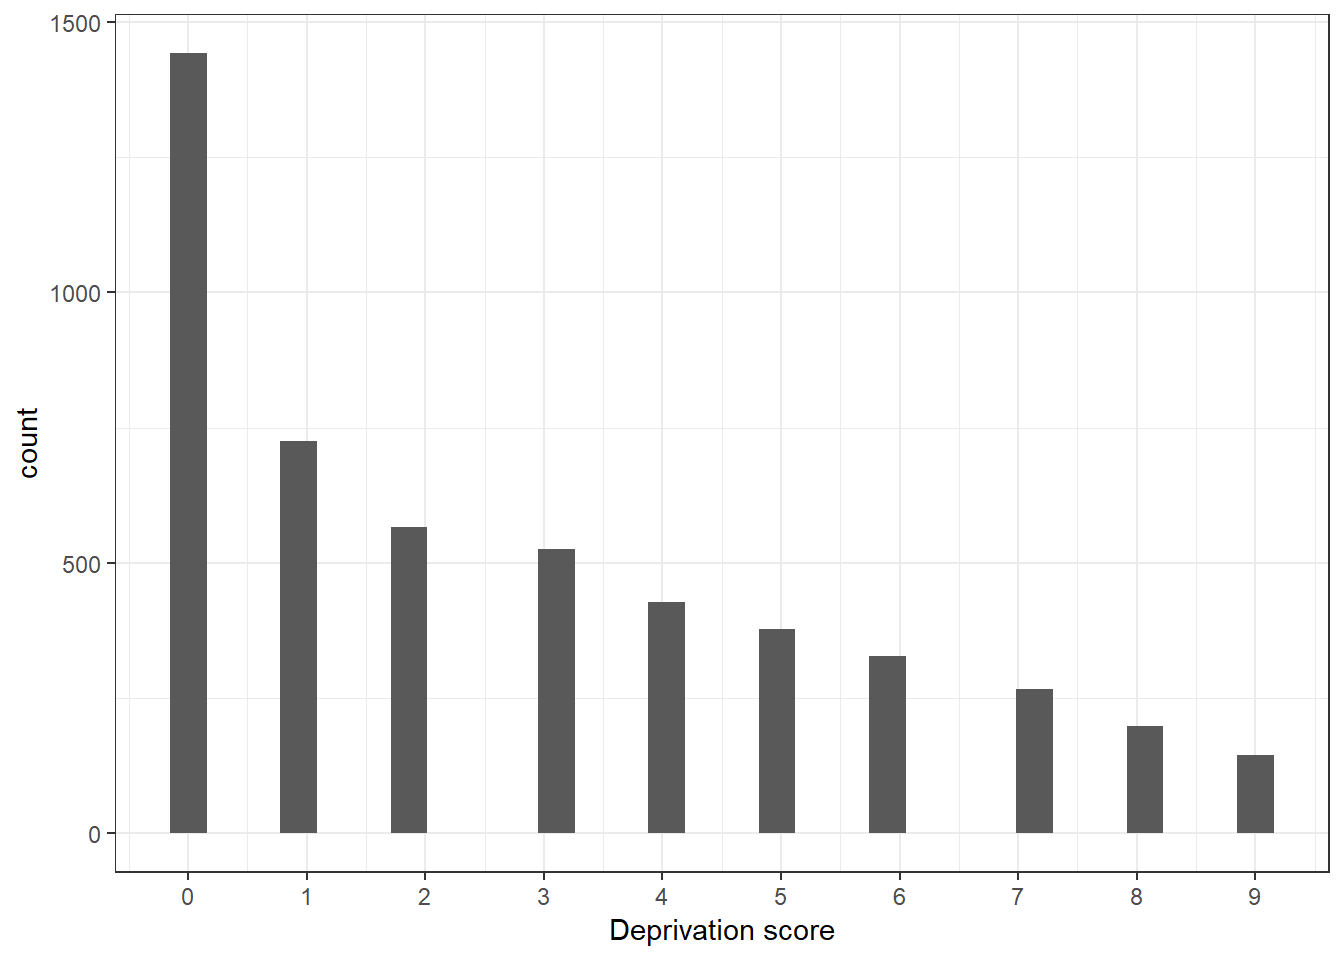
\includegraphics{PM_Book_files/figure-latex/depscore-1.png}
\caption{\label{fig:depscore}This is the histogram of the deprivation score. It shows the number of people by the equally weighted deprivation count.}
\end{figure}

Now we can check the proportion of people deprived of each indicator as follows:

\begin{Shaded}
\begin{Highlighting}[]
\NormalTok{dep_prop<-}\KeywordTok{unlist}\NormalTok{(}\KeywordTok{lapply}\NormalTok{(Rel_MD_}\DecValTok{1}\NormalTok{, }\ControlFlowTok{function}\NormalTok{(x) }\KeywordTok{mean}\NormalTok{(x)))}
\NormalTok{dep_prop<-}\KeywordTok{round}\NormalTok{(dep_prop[}\DecValTok{1}\OperatorTok{:}\DecValTok{9}\NormalTok{]}\OperatorTok{*}\DecValTok{100}\NormalTok{,}\DecValTok{0}\NormalTok{)}
\NormalTok{dep_prop}
\end{Highlighting}
\end{Shaded}

\begin{verbatim}
## x1 x2 x3 x4 x5 x6 x7 x8 x9 
## 50 29 16 49 29 16 45 26 16
\end{verbatim}

\hypertarget{Chapter-3-expoverel}{%
\subsection{Exploratory (non-model based) estimation of overall reliability}\label{Chapter-3-expoverel}}

ow that we have familiarised with the data ourselves we can proceed to check the reliability of this scale. Reliability concerns with the homogeneity of a scale and its capacity to produce consistent rankings of a population. We will start by estimating the overall reliability of our scale using the \texttt{psych} package (Revelle, \protect\hyperlink{ref-Revelle2014}{2014}). This is a comprehensive R-package to estimate different reliability statistics (\(\alpha\), \(\beta\), \(\omega\) and \(\omega_h\)) under different changing conditions. The \texttt{psych} package can be used for exploratory and confirmatory settings for both unidimensional and multidimensional measures. This book focuses on confirmatory measurement models and to introduce the estimation of overall reliability we will rely on the simplest way to estimate the homogeneity of a scale using the simulated data set. This will be further developed and the next section shows how \texttt{psych} interacts with another R-package \texttt{lavaan} to estimate \(\omega\) and \(\omega_h\) from a confirmatory factor model (Rosseel, \protect\hyperlink{ref-Rosseel2012}{2012}).

The \texttt{pysch} package permits estimating \(\alpha\) and \(\omega\) using the same function (\texttt{omega}). The package has several options but we know that there are three dimensions and one higher order factor and these values match the defaults of the \texttt{omega} function. It is important to bear in mind that in this simple case the value of \(\omega\) is approximated with an Exploratory Factor Analysis (EFA). Below is shown how to do it with a confirmatory model.

After applying the \texttt{omega()} to our nine indicators, there will be different objects that store information with the results of the analysis. We will focus on the overall estimate of \(\alpha\) and \(\omega\) as here we are interested in knowing the homogeneity of our scale. We can appreciate below that both values are high (\(\geq.8\)) (See \emph{ref} for an explanation) and suggest that the scale is highly reliable. In this case, \(\alpha<\omega\) indicating that this scale violates \(\tau\) equivalence (equality of loadings).

\begin{Shaded}
\begin{Highlighting}[]
\CommentTok{# install.packages("psych")}
\KeywordTok{require}\NormalTok{(psych)}
\NormalTok{omega_exp1<-}\KeywordTok{omega}\NormalTok{(Rel_MD_}\DecValTok{1}\NormalTok{[,}\KeywordTok{c}\NormalTok{(}\DecValTok{3}\OperatorTok{:}\DecValTok{9}\NormalTok{)])}
\NormalTok{rel_uni_exp<-}\KeywordTok{data.frame}\NormalTok{(}\DataTypeTok{omega_exp1=}\NormalTok{omega_exp1}\OperatorTok{$}\NormalTok{omega.tot, }
                        \DataTypeTok{alpha=}\NormalTok{omega_exp1}\OperatorTok{$}\NormalTok{alpha)}
\NormalTok{rel_uni_exp}
\end{Highlighting}
\end{Shaded}

\begin{verbatim}
##   omega_exp1     alpha
## 1  0.8599319 0.8127129
\end{verbatim}

Both \(\alpha\) and \(\omega\) are easily estimated with the \texttt{psych} package. However, the previous example was pretty straightforward in that all the indicators are well-behaved. Thus to gain a deeper understanding of reliability and population classification we will check what happens when one has indicators that reduce reliability. This can be done by adding noise to our measure. We will generate two uncorrelated indicators and substitute x10 and x11 for the indicators x1 and x2.
Once the we have introduce some noise to our measure we will estimate a new deprivation score using the two new indicators and dropping x1 and x2. The result is shown below. Then we can apply \texttt{omega()} to the new matrix that includes V1 and v1 and excludes x1 and x2. Reliability has drop slightly but enough to raise concerns as both \(\omega\) and \(\alpha\) are below the rules of thumb drawn from a Monte Carlo experiment.

\begin{Shaded}
\begin{Highlighting}[]
\CommentTok{#Computing deprivation score with uncorrelated items}
\NormalTok{Rel_MD_}\DecValTok{1}\OperatorTok{$}\NormalTok{ds_ur<-}\KeywordTok{rowSums}\NormalTok{(Rel_MD_}\DecValTok{1}\NormalTok{[,}\KeywordTok{c}\NormalTok{(}\DecValTok{3}\OperatorTok{:}\DecValTok{11}\NormalTok{)])}
\NormalTok{Rel_MD_}\DecValTok{1}\NormalTok{[}\DecValTok{1}\OperatorTok{:}\DecValTok{10}\NormalTok{,}\KeywordTok{c}\NormalTok{(}\DecValTok{16}\NormalTok{,}\DecValTok{17}\NormalTok{)]}
\end{Highlighting}
\end{Shaded}

\begin{verbatim}
##    hh_members ds
## 1           2  4
## 2           1  0
## 3           1  1
## 4           2  3
## 5           2  1
## 6           1  1
## 7           1  2
## 8           2  1
## 9           2  7
## 10          2  0
\end{verbatim}

\begin{Shaded}
\begin{Highlighting}[]
\CommentTok{#Now reliability drops}
\NormalTok{omega_unr_exp<-}\KeywordTok{omega}\NormalTok{(Rel_MD_}\DecValTok{1}\NormalTok{[,}\KeywordTok{c}\NormalTok{(}\DecValTok{3}\OperatorTok{:}\DecValTok{11}\NormalTok{)])}
\NormalTok{unrel_uni_exp<-}\KeywordTok{data.frame}\NormalTok{(}\DataTypeTok{omega_exp=}\NormalTok{omega_unr_exp}\OperatorTok{$}\NormalTok{omega.tot, }
                          \DataTypeTok{alpha=}\NormalTok{omega_unr_exp}\OperatorTok{$}\NormalTok{alpha)}
\NormalTok{unrel_uni_exp}
\end{Highlighting}
\end{Shaded}

\begin{verbatim}
##   omega_exp    alpha
## 1  0.799405 0.738685
\end{verbatim}

What is the impact of introducing the two uncorrelated indicators? From theory is known that losses in reliability affect the consistency of population classification. We can check if this theory holds by looking at the correlation of different rankings that are produce from different measures. For this experiment, first, we will estimate the omega values using different combinations of items (in all case we have the seven items from the reliable measure x1-x9).

\begin{Shaded}
\begin{Highlighting}[]
\NormalTok{omega_exp2<-}\KeywordTok{omega}\NormalTok{(Rel_MD_}\DecValTok{1}\NormalTok{[,}\KeywordTok{c}\NormalTok{(}\DecValTok{3}\OperatorTok{:}\DecValTok{9}\NormalTok{)])}
\NormalTok{omega_exp3<-}\KeywordTok{omega}\NormalTok{(Rel_MD_}\DecValTok{1}\NormalTok{[,}\KeywordTok{c}\NormalTok{(}\DecValTok{1}\NormalTok{,}\DecValTok{2}\NormalTok{,}\DecValTok{4}\NormalTok{,}\DecValTok{5}\NormalTok{,}\DecValTok{7}\NormalTok{,}\DecValTok{8}\NormalTok{)])}
\NormalTok{omega_exp4<-}\KeywordTok{omega}\NormalTok{(Rel_MD_}\DecValTok{1}\NormalTok{[,}\KeywordTok{c}\NormalTok{(}\DecValTok{2}\NormalTok{,}\DecValTok{3}\NormalTok{,}\DecValTok{5}\NormalTok{,}\DecValTok{6}\NormalTok{,}\DecValTok{8}\NormalTok{,}\DecValTok{9}\NormalTok{)])}
\NormalTok{omega_exp5<-}\KeywordTok{omega}\NormalTok{(Rel_MD_}\DecValTok{1}\NormalTok{[,}\KeywordTok{c}\NormalTok{(}\DecValTok{1}\NormalTok{,}\DecValTok{3}\NormalTok{,}\DecValTok{4}\NormalTok{,}\DecValTok{6}\NormalTok{,}\DecValTok{7}\NormalTok{,}\DecValTok{9}\NormalTok{)])}


\NormalTok{omegas_exp<-}\KeywordTok{data.frame}\NormalTok{(}\DataTypeTok{omega_exp1=}\NormalTok{omega_exp1}\OperatorTok{$}\NormalTok{omega.tot, }
                       \DataTypeTok{omega_exp2=}\NormalTok{omega_exp2}\OperatorTok{$}\NormalTok{omega.tot,}
                       \DataTypeTok{omega_exp3=}\NormalTok{omega_exp3}\OperatorTok{$}\NormalTok{omega.tot, }
                       \DataTypeTok{omega_exp4=}\NormalTok{omega_exp4}\OperatorTok{$}\NormalTok{omega.tot, }
                       \DataTypeTok{omega_exp5=}\NormalTok{omega_exp5}\OperatorTok{$}\NormalTok{omega.tot, }
                       \DataTypeTok{omega_unrel=}\NormalTok{omega_unr_exp}\OperatorTok{$}\NormalTok{omega.tot)}
\end{Highlighting}
\end{Shaded}

We then can compare the omega values of each measure. The theory holds for this example. We see that the lowest reliability scale is the one that incorporates V1 and V2. The measures with only seven items have higher reliability. This is a very important lesson as poverty researchers sometimes keep unreliable indicators in their scales and the consequence will be a heavy loss in reliability.

\begin{Shaded}
\begin{Highlighting}[]
\KeywordTok{t}\NormalTok{(omegas_exp)}
\end{Highlighting}
\end{Shaded}

\begin{verbatim}
##                  [,1]
## omega_exp1  0.8599319
## omega_exp2  0.8599319
## omega_exp3  0.8779016
## omega_exp4  0.8543497
## omega_exp5  0.8441886
## omega_unrel 0.7994050
\end{verbatim}

The second prediction of reliability theory is that the population orderings are consistent for high reliability values. One way to check this is by estimating the correlation among the different deprivation scores. Again, the theory holds for this simple exercise, the measure with higher \(\omega\) are highly correlated. The correlation of the unreliable measure seems still high, however, when \(\omega<.8\) we could expect to see a classification error \(>5\%\) which might be very worrying when put into perspective. If the poverty rate is \(20\%\) and the classification error is \(5\%\) it would mean that potentially a \(25\%\) of the poor are mistakenly classified (Nájera, \protect\hyperlink{ref-Najera2018}{2018}).

\begin{Shaded}
\begin{Highlighting}[]
\NormalTok{Rel_MD_}\DecValTok{1}\OperatorTok{$}\NormalTok{ds_r2<-}\KeywordTok{rowSums}\NormalTok{(Rel_MD_}\DecValTok{1}\NormalTok{[,}\KeywordTok{c}\NormalTok{(}\DecValTok{3}\OperatorTok{:}\DecValTok{9}\NormalTok{)])}
\NormalTok{Rel_MD_}\DecValTok{1}\OperatorTok{$}\NormalTok{ds_r3<-}\KeywordTok{rowSums}\NormalTok{(Rel_MD_}\DecValTok{1}\NormalTok{[,}\KeywordTok{c}\NormalTok{(}\DecValTok{1}\NormalTok{,}\DecValTok{2}\NormalTok{,}\DecValTok{4}\NormalTok{,}\DecValTok{5}\NormalTok{,}\DecValTok{7}\NormalTok{,}\DecValTok{8}\NormalTok{)])}
\NormalTok{Rel_MD_}\DecValTok{1}\OperatorTok{$}\NormalTok{ds_r4<-}\KeywordTok{rowSums}\NormalTok{(Rel_MD_}\DecValTok{1}\NormalTok{[,}\KeywordTok{c}\NormalTok{(}\DecValTok{2}\NormalTok{,}\DecValTok{3}\NormalTok{,}\DecValTok{5}\NormalTok{,}\DecValTok{6}\NormalTok{,}\DecValTok{8}\NormalTok{,}\DecValTok{9}\NormalTok{)])}
\NormalTok{Rel_MD_}\DecValTok{1}\OperatorTok{$}\NormalTok{ds_r5<-}\KeywordTok{rowSums}\NormalTok{(Rel_MD_}\DecValTok{1}\NormalTok{[,}\KeywordTok{c}\NormalTok{(}\DecValTok{1}\NormalTok{,}\DecValTok{3}\NormalTok{,}\DecValTok{4}\NormalTok{,}\DecValTok{6}\NormalTok{,}\DecValTok{7}\NormalTok{,}\DecValTok{9}\NormalTok{)])}

\NormalTok{ds.m<-(Rel_MD_}\DecValTok{1}\NormalTok{[,}\KeywordTok{c}\NormalTok{(}\DecValTok{16}\OperatorTok{:}\DecValTok{21}\NormalTok{)])}
\NormalTok{ds.cor<-}\KeywordTok{cor}\NormalTok{(ds.m)}
\NormalTok{ds.cor}
\end{Highlighting}
\end{Shaded}

\begin{verbatim}
##            hh_members        ds     ds_ur     ds_r2     ds_r3     ds_r4
## hh_members  1.0000000 0.4330385 0.3945498 0.4077791 0.4422686 0.3777748
## ds          0.4330385 1.0000000 0.9272651 0.9684719 0.9764524 0.9523882
## ds_ur       0.3945498 0.9272651 1.0000000 0.9520979 0.8899044 0.8941369
## ds_r2       0.4077791 0.9684719 0.9520979 1.0000000 0.9284786 0.9370200
## ds_r3       0.4422686 0.9764524 0.8899044 0.9284786 1.0000000 0.8875033
## ds_r4       0.3777748 0.9523882 0.8941369 0.9370200 0.8875033 1.0000000
\end{verbatim}

\hypertarget{model-based-estimation-of-overall-reliability}{%
\subsection{Model-based estimation of overall reliability}\label{model-based-estimation-of-overall-reliability}}

The ideal workflow in poverty measurement leads to a specification of a model. Different models suggest that poverty is multidimensional and hierarchical (See Section \ref{Chapter-1-dimensions}). Therefore, the interest is in both estimates of reliability: overall and hierarchical omega (\(\omega\) and \(\omega_h\)). Both can be estimated from an EFA using the R-package ``psych''. However, this book is an attempt to encourage poverty researchers to walk toward the production and assessment of theoretical models. To estimate reliability for a pre-specified model, it is necessary to use Confirmatory Factor Analysis (CFA). Given a pattern loading specification, a CFA will estimate the different parameters of the model. Section \ref{Chapter-3-measuresrel} showed the formulas to estimate both \(\omega\) and \(\omega_h\). Item-factor loadings and the residuals of the model are the key parameters for the estimation of both reliability statistics (See equation \eqref{eq:omega}).

In the following we will show how in both \textbf{Mplus} and \textbf{R} is possible to estimate \(\omega\) and \(\omega_h\). We will start with R and for this purpose we need the \texttt{lavaan} package (Rosseel, \protect\hyperlink{ref-Rosseel2012}{2012}). This package comprises a series of functions to estimate different kinds of latent variable models such as measurement and analytic models like Structural Equation Models (SEM). Once the CFA model is fitted with the R-package \texttt{lavaan}, the function \texttt{omegaFromSem()} of the \texttt{psych} R-package can be used to estimate \(\omega\) and \(\omega_h\). However, we will show how this can be done by hand to gain insight of the differences between the two reliability statistics and to operationalise the process using the \textbf{Mplus} estimates.

\begin{Shaded}
\begin{Highlighting}[]
\CommentTok{#Omega from Sem}
\KeywordTok{library}\NormalTok{(lavaan)}
\CommentTok{# We first specify the model}
\NormalTok{MD_model <-}\StringTok{ ' h =~ +x1+x2+x3+x4+x5+x6+x7+x8+x9 }
\StringTok{                F1=~  + x7 + x8 + x9        }
\StringTok{                F2=~  + x4 + x5 + x6         }
\StringTok{                F3=~  + x1 + x2 + x3}
\StringTok{                h  ~~ 0*F1}
\StringTok{                h  ~~ 0*F2}
\StringTok{                h  ~~ 0*F3}
\StringTok{                F1 ~~ 0*F2}
\StringTok{                F2 ~~ 0*F3}
\StringTok{                F1 ~~ 0*F3}

\StringTok{'}
\end{Highlighting}
\end{Shaded}

To fit the CFA model we will use \texttt{sem} function which has been harmonised with the functions \texttt{cfa} and \texttt{lavaan}. The function requires specifying the measurement model (MD\_model), the data, the kind of variables we have (in this case categorical) and we will request standardised loadings with \texttt{std.lv=TRUE}.

\begin{Shaded}
\begin{Highlighting}[]
\NormalTok{fit <-}\StringTok{ }\KeywordTok{sem}\NormalTok{(MD_model, }\DataTypeTok{data =}\NormalTok{ Rel_MD_}\DecValTok{1}\NormalTok{, }
           \DataTypeTok{ordered=}\KeywordTok{c}\NormalTok{(}\StringTok{"x1"}\NormalTok{,}\StringTok{"x2"}\NormalTok{,}\StringTok{"x3"}\NormalTok{,}\StringTok{"x4"}\NormalTok{,}\StringTok{"x5"}\NormalTok{,}
                     \StringTok{"x6"}\NormalTok{,}\StringTok{"x7"}\NormalTok{,}\StringTok{"x8"}\NormalTok{,}\StringTok{"x9"}\NormalTok{),}
           \DataTypeTok{std.lv=}\OtherTok{TRUE}\NormalTok{)}
\CommentTok{# The command below is to check the output (We will check this in the }
\CommentTok{#next section and validity chapter)}
\CommentTok{#summary(fit, fit.measures=TRUE, rsquare=TRUE, standardized=TRUE)}
\end{Highlighting}
\end{Shaded}

Both \(\omega\) and \(\omega_h\) can be manually calculated. There are two main parameters one needs for their computation: factor loadings from the indicators to the overall factor (\(\lambda_h\)), to each dimension (\(\lambda_j\)) and the error. This can be easily extracted from the fit object as follows:

\begin{Shaded}
\begin{Highlighting}[]
\NormalTok{lambdas<-}\KeywordTok{as.data.frame}\NormalTok{(fit}\OperatorTok{@}\NormalTok{Model}\OperatorTok{@}\NormalTok{GLIST}\OperatorTok{$}\NormalTok{lambda)}
\NormalTok{error<-}\KeywordTok{colSums}\NormalTok{(fit}\OperatorTok{@}\NormalTok{Model}\OperatorTok{@}\NormalTok{GLIST}\OperatorTok{$}\NormalTok{theta)}
\end{Highlighting}
\end{Shaded}

The then the square of the sum of the loadings (\(\lambda_h\)) and (\(\lambda_j\)) is taken as well as the sum of the error. The we can compute both \(\omega\) and \(\omega_h\) using equation \eqref{eq:omega} and \eqref{eq:omegah}.

\begin{Shaded}
\begin{Highlighting}[]
\NormalTok{Slambda_}\DecValTok{2}\NormalTok{<-}\KeywordTok{sum}\NormalTok{(lambdas[}\DecValTok{1}\NormalTok{])}\OperatorTok{^}\DecValTok{2} \OperatorTok{+}\StringTok{ }\KeywordTok{sum}\NormalTok{(lambdas[}\DecValTok{2}\NormalTok{])}\OperatorTok{^}\DecValTok{2} \OperatorTok{+}\StringTok{ }
\StringTok{           }\KeywordTok{sum}\NormalTok{(lambdas[}\DecValTok{3}\NormalTok{])}\OperatorTok{^}\DecValTok{2} \OperatorTok{+}\StringTok{ }\KeywordTok{sum}\NormalTok{(lambdas[}\DecValTok{4}\NormalTok{])}\OperatorTok{^}\DecValTok{2}
\NormalTok{error <-}\StringTok{ }\KeywordTok{sum}\NormalTok{(error)}

\NormalTok{omega_t <-}\StringTok{ }\NormalTok{Slambda_}\DecValTok{2} \OperatorTok{/}\StringTok{ }\NormalTok{(Slambda_}\DecValTok{2}\OperatorTok{+}\NormalTok{error)}
\NormalTok{omega_h <-}\StringTok{ }\KeywordTok{sum}\NormalTok{(lambdas[}\DecValTok{1}\NormalTok{])}\OperatorTok{^}\DecValTok{2} \OperatorTok{/}\StringTok{ }\NormalTok{(Slambda_}\DecValTok{2}\OperatorTok{+}\NormalTok{error)}
\NormalTok{omegamanual<-}\KeywordTok{c}\NormalTok{(}\DataTypeTok{omega_h=}\NormalTok{omega_h,}\DataTypeTok{omega_t=}\NormalTok{omega_t)}
\NormalTok{omegamanual}
\end{Highlighting}
\end{Shaded}

\begin{verbatim}
##   omega_h   omega_t 
## 0.8445022 0.9707344
\end{verbatim}

Fortunately, there is an R function from the ``psych'' package that does this for us. Once the model has been fitted, we apply the function \texttt{omegaFromSem()} to request the estimates and store the estimates of both \(\omega\) and \(\omega_h\) in the \texttt{omegasem} object. The results indicate high overall reliability and high reliability after considering the multidimensional features of the scale.

\begin{Shaded}
\begin{Highlighting}[]
\NormalTok{omegasem<-}\KeywordTok{omegaFromSem}\NormalTok{(fit)}
\NormalTok{omegasem<-}\KeywordTok{c}\NormalTok{(}\DataTypeTok{omega_h=}\NormalTok{omegasem}\OperatorTok{$}\NormalTok{omega,}
            \DataTypeTok{omega_t=}\NormalTok{omegasem}\OperatorTok{$}\NormalTok{omega.tot)}
\NormalTok{omegasem}
\end{Highlighting}
\end{Shaded}

\begin{verbatim}
##   omega_h   omega_t 
## 0.8446990 0.9707276
\end{verbatim}

The R package ``mplusAutomation'' is an excellent alternative to automate Mplus from R (Hallquist \& Wiley, \protect\hyperlink{ref-Hallquist2018}{2018}). We can create within R an Mplus object as follows using the function \texttt{mplusObject()}. The syntax is the standard Mplus syntax to fit a model. As with \texttt{lavaan} we will fit a bi-factor model. We will store the syntax in the object \texttt{test}.

\begin{Shaded}
\begin{Highlighting}[]
\NormalTok{test <-}\StringTok{ }\KeywordTok{mplusObject}\NormalTok{(}
\DataTypeTok{TITLE =} \StringTok{"Bi-factor model CFA;"}\NormalTok{,}
   \DataTypeTok{VARIABLE =} \StringTok{"}
\StringTok{     NAMES = x1-x9 resources educ_yr occupation class;}
\StringTok{     CATEGORICAL = x1-x9;}
\StringTok{     USEVARIABLES = x1-x9;"}\NormalTok{,}
   \DataTypeTok{ANALYSIS =} \StringTok{"ESTIMATOR = wlsmv;}
\StringTok{              PROCESS = 4;"}\NormalTok{,}

\DataTypeTok{MODEL =} \StringTok{"f1 by x1-x3;}
\StringTok{  f2 by x4-x6;}
\StringTok{  f3 by x7-x9;}
\StringTok{  h by x1 x2 x3 x4 x4 x5 x6 x7 x8 x9;}
\StringTok{  F1 with F2@0;}
\StringTok{  F2 with F3@0;}
\StringTok{  F3 with F1@0;}
\StringTok{  h with f1@0;}
\StringTok{  h with f2@0;}
\StringTok{  h with f3@0;"}\NormalTok{,}

\DataTypeTok{OUTPUT =} \StringTok{"std stdyx;"}\NormalTok{)}
\end{Highlighting}
\end{Shaded}

To write the \texttt{test} object as an "*.inp" Mplus syntax file, we will use the function \texttt{mplusModeler()}. This function permits estimating the model directly using the option \texttt{run}.

\begin{Shaded}
\begin{Highlighting}[]
\NormalTok{res <-}\StringTok{ }\KeywordTok{mplusModeler}\NormalTok{(test, }\DataTypeTok{modelout =} \StringTok{"rel_CFA_2.inp"}\NormalTok{, }
                    \DataTypeTok{writeData =} \StringTok{"never"}\NormalTok{, }\DataTypeTok{hashfilename =} \OtherTok{FALSE}\NormalTok{, }
                    \DataTypeTok{dataout=}\StringTok{"Rel_MD_data_1_1.dat"}\NormalTok{, }\DataTypeTok{run =}\NormalTok{ 1L)}
\end{Highlighting}
\end{Shaded}

\begin{verbatim}
## 
## Running model: rel_CFA_2.inp 
## System command: C:\WINDOWS\system32\cmd.exe /c cd "." && "Mplus" "rel_CFA_2.inp" 
## Reading model:  rel_CFA_2.out
\end{verbatim}

Once the model has been run, we can import the output using the function \texttt{readModels()}. We will explore the full output in the next chapter as for now we will focus in the estimation of \(\omega\) and \(\omega_h\). The factor loadings of the Bi-factor model are stored in a list (parameters). We request the standardised estimates as we did with \texttt{lavaan}. We also can request the error from the `\texttt{r2} object in the parameters list. Once we have the parameters we need we can proceed as above to estimate the reliability statistics. We see that we could replicate the results from \texttt{lavaan}.

\begin{Shaded}
\begin{Highlighting}[]
\NormalTok{REL_CFA_}\DecValTok{2}\NormalTok{<-}\KeywordTok{readModels}\NormalTok{(}\DataTypeTok{filefilter =}\StringTok{"rel_CFA_2"}\NormalTok{)}
\end{Highlighting}
\end{Shaded}

\begin{verbatim}
## Reading model:  C:/Proyectos Investigacion/PM Book/rel_cfa_2.out
\end{verbatim}

\begin{Shaded}
\begin{Highlighting}[]
\NormalTok{lambdas<-REL_CFA_}\DecValTok{2}\OperatorTok{$}\NormalTok{parameters}\OperatorTok{$}\NormalTok{std.standardized[}\DecValTok{1}\OperatorTok{:}\DecValTok{18}\NormalTok{,}\DecValTok{1}\OperatorTok{:}\DecValTok{3}\NormalTok{]}
\NormalTok{error<-REL_CFA_}\DecValTok{2}\OperatorTok{$}\NormalTok{parameters}\OperatorTok{$}\NormalTok{r2[}\DecValTok{6}\NormalTok{]}

\NormalTok{lambda_}\DecValTok{2}\NormalTok{<-}\KeywordTok{sum}\NormalTok{(lambdas[}\DecValTok{10}\OperatorTok{:}\DecValTok{18}\NormalTok{,}\DecValTok{3}\NormalTok{])}\OperatorTok{^}\DecValTok{2} \OperatorTok{+}\StringTok{ }\KeywordTok{sum}\NormalTok{(lambdas[}\DecValTok{1}\OperatorTok{:}\DecValTok{3}\NormalTok{,}\DecValTok{3}\NormalTok{])}\OperatorTok{^}\DecValTok{2} \OperatorTok{+}\StringTok{ }
\StringTok{          }\KeywordTok{sum}\NormalTok{(lambdas[}\DecValTok{4}\OperatorTok{:}\DecValTok{6}\NormalTok{,}\DecValTok{3}\NormalTok{])}\OperatorTok{^}\DecValTok{2} \OperatorTok{+}\StringTok{ }\KeywordTok{sum}\NormalTok{(lambdas[}\DecValTok{7}\OperatorTok{:}\DecValTok{9}\NormalTok{,}\DecValTok{3}\NormalTok{])}\OperatorTok{^}\DecValTok{2}
\NormalTok{error <-}\StringTok{ }\KeywordTok{sum}\NormalTok{(error)}

\NormalTok{omega_t <-}\StringTok{ }\NormalTok{lambda_}\DecValTok{2} \OperatorTok{/}\StringTok{ }\NormalTok{(lambda_}\DecValTok{2}\OperatorTok{+}\NormalTok{error)}
\NormalTok{omega_h <-}\StringTok{ }\KeywordTok{sum}\NormalTok{(lambdas[}\DecValTok{10}\OperatorTok{:}\DecValTok{18}\NormalTok{,}\DecValTok{3}\NormalTok{])}\OperatorTok{^}\DecValTok{2} \OperatorTok{/}\StringTok{ }\NormalTok{(lambda_}\DecValTok{2}\OperatorTok{+}\NormalTok{error)}

\NormalTok{omega_t}
\end{Highlighting}
\end{Shaded}

\begin{verbatim}
## [1] 0.9707333
\end{verbatim}

\begin{Shaded}
\begin{Highlighting}[]
\NormalTok{omega_h}
\end{Highlighting}
\end{Shaded}

\begin{verbatim}
## [1] 0.8445348
\end{verbatim}

\hypertarget{overall-reliability-and-population-orderings}{%
\subsection{Overall reliability and population orderings}\label{overall-reliability-and-population-orderings}}

One of the predictions of measurement theory is that reliability leads to consistent population orderings, i.e.~poor people will have high deprivation scores and not poor people will have low deprivation scores (see Table \label{tab:relentropy}). We illustrated this point using the correlation between the different deprivation scores corresponding to diverse levels of overall reliabilities. We can follow up that example by looking at the values of the latent variable for the multidimensional reliable measure (Rel\_MD\_1). After fitting the CFA model we just can simply use the function \texttt{predict()} to obtain the Maximum Likelihood estimates of the latent variable. Then we can merge these values with our data set. The prediction will generate four estimates for the latent variables. The overall factor (h) and the values for the three dimensions.

\begin{Shaded}
\begin{Highlighting}[]
\NormalTok{factor_scores<-}\KeywordTok{predict}\NormalTok{(fit)}
\NormalTok{Rel_MD_}\DecValTok{1}\NormalTok{<-}\KeywordTok{cbind}\NormalTok{(Rel_MD_}\DecValTok{1}\NormalTok{,factor_scores)}
\KeywordTok{head}\NormalTok{(Rel_MD_}\DecValTok{1}\NormalTok{[,}\KeywordTok{c}\NormalTok{(}\DecValTok{21}\OperatorTok{:}\DecValTok{24}\NormalTok{)])}
\end{Highlighting}
\end{Shaded}

\begin{verbatim}
##   ds_r4 ds_r5          h          F1
## 1     2     3  0.4475885 -0.81293477
## 2     0     0 -0.6781638 -0.08627376
## 3     0     1 -0.2440620 -0.28822588
## 4     1     2  0.2851351  0.13806885
## 5     0     1 -0.2207057 -0.30252106
## 6     0     1 -0.2207057 -0.30252106
\end{verbatim}

To contrast the values of the reliable multidimensional measure with the values of an slitghly less reliable measure we will fit a new model. As in the previous example (Section @ref(\#Chapter-3-expoverel)), we will replace the first two indicators x1 and x2 by x10 and x11. Both load into the first factor (f1). The estimates are stored in a different object (fit\_ur) and estimate the factor scores using the \texttt{predict()} function. Finally we inspect the values.

\begin{Shaded}
\begin{Highlighting}[]
\CommentTok{## We first specify the model}
\NormalTok{MD_model <-}\StringTok{ ' h =~ +x10+x11+x3+x4+x5+x6+x7+x8+x9 }
\StringTok{                F1=~  + x7 + x8 + x9        }
\StringTok{                F2=~  + x4 + x5 + x6         }
\StringTok{                F3=~  + x10 + x11 + x3}
\StringTok{                h  ~~ 0*F1}
\StringTok{                h  ~~ 0*F2}
\StringTok{                h  ~~ 0*F3}
\StringTok{                F1 ~~ 0*F2}
\StringTok{                F2 ~~ 0*F3}
\StringTok{                F1 ~~ 0*F3}

\StringTok{'}

\NormalTok{fit_ur <-}\StringTok{ }\KeywordTok{sem}\NormalTok{(MD_model, }\DataTypeTok{data =}\NormalTok{ Rel_MD_}\DecValTok{1}\NormalTok{, }
           \DataTypeTok{ordered=}\KeywordTok{c}\NormalTok{(}\StringTok{"x10"}\NormalTok{,}\StringTok{"x11"}\NormalTok{,}\StringTok{"x3"}\NormalTok{,}\StringTok{"x4"}\NormalTok{,}\StringTok{"x5"}\NormalTok{,}\StringTok{"x6"}\NormalTok{,}\StringTok{"x7"}\NormalTok{,}\StringTok{"x8"}\NormalTok{,}\StringTok{"x9"}\NormalTok{),}
           \DataTypeTok{std.lv=}\OtherTok{TRUE}\NormalTok{)}
\NormalTok{factor_scores_ur<-}\KeywordTok{predict}\NormalTok{(fit_ur)}
\KeywordTok{colnames}\NormalTok{(factor_scores_ur)[}\DecValTok{1}\OperatorTok{:}\DecValTok{4}\NormalTok{]<-}\KeywordTok{c}\NormalTok{(}\StringTok{"hur"}\NormalTok{,}\StringTok{"F1ur"}\NormalTok{,}\StringTok{"F2ur"}\NormalTok{,}\StringTok{"F3ur"}\NormalTok{)}
\NormalTok{Rel_MD_}\DecValTok{1}\NormalTok{<-}\KeywordTok{cbind}\NormalTok{(Rel_MD_}\DecValTok{1}\NormalTok{,factor_scores_ur)}
\KeywordTok{head}\NormalTok{(Rel_MD_}\DecValTok{1}\NormalTok{[,}\KeywordTok{c}\NormalTok{(}\DecValTok{25}\OperatorTok{:}\DecValTok{28}\NormalTok{)])}
\end{Highlighting}
\end{Shaded}

\begin{verbatim}
##           F2         F3         hur       F1ur
## 1 -0.1296229  1.2478407  0.38436469 -0.7563179
## 2 -0.1536510 -0.1720003 -0.59656764 -0.1126966
## 3  0.5290560 -0.3986557 -0.10512455 -0.3763817
## 4 -0.7559100  0.7442695 -0.05228111  0.4723843
## 5 -0.3910445  0.4514504 -0.50856087 -0.1482380
## 6 -0.3910445  0.4514504 -0.59656764 -0.1126966
\end{verbatim}

To assess the consistency of both multidimensional scales we will plot the latent factor values by the deprivation score. Figure\textasciitilde\ref{fig:fsdesrel} shows that the factor scores are very similar within each deprivation group. For each deprivation score we find very different factor scores, indicating that the deprivation scores is a good measure to rank and split the population according to the severity of deprivation. In contrast, figure\textasciitilde@ref\{(fig:fsdesunrel) show that although there is relationship between the deprivation score and factor scores, this relationship is more noisy. Not only there is much more variability within each deprivation group but also there is some overlap. That means that if we use some cut off to split the poor from the not poor based on a deprivation score, we will be more likely to confound both groups. In this case, the mixing of groups is not that dramatic as the scale is still somewhat reliable, but it could be very noisy for less reliable scales.

\begin{Shaded}
\begin{Highlighting}[]
\KeywordTok{require}\NormalTok{(ggplot2)}
\NormalTok{g <-}\StringTok{ }\KeywordTok{ggplot}\NormalTok{(Rel_MD_}\DecValTok{1}\NormalTok{, }\KeywordTok{aes}\NormalTok{(}\KeywordTok{as.factor}\NormalTok{(ds), h))}
\NormalTok{g }\OperatorTok{+}\StringTok{ }\KeywordTok{geom_boxplot}\NormalTok{(}\DataTypeTok{varwidth=}\NormalTok{T) }\OperatorTok{+}\StringTok{ }
\StringTok{    }\KeywordTok{labs}\NormalTok{(}\DataTypeTok{x=}\StringTok{"Deprivation score. Reliable"}\NormalTok{,}
         \DataTypeTok{y=}\StringTok{"Factor score (Latent variable)"}\NormalTok{) }\OperatorTok{+}\StringTok{ }\KeywordTok{theme_bw}\NormalTok{()}
\end{Highlighting}
\end{Shaded}

\begin{figure}
\centering
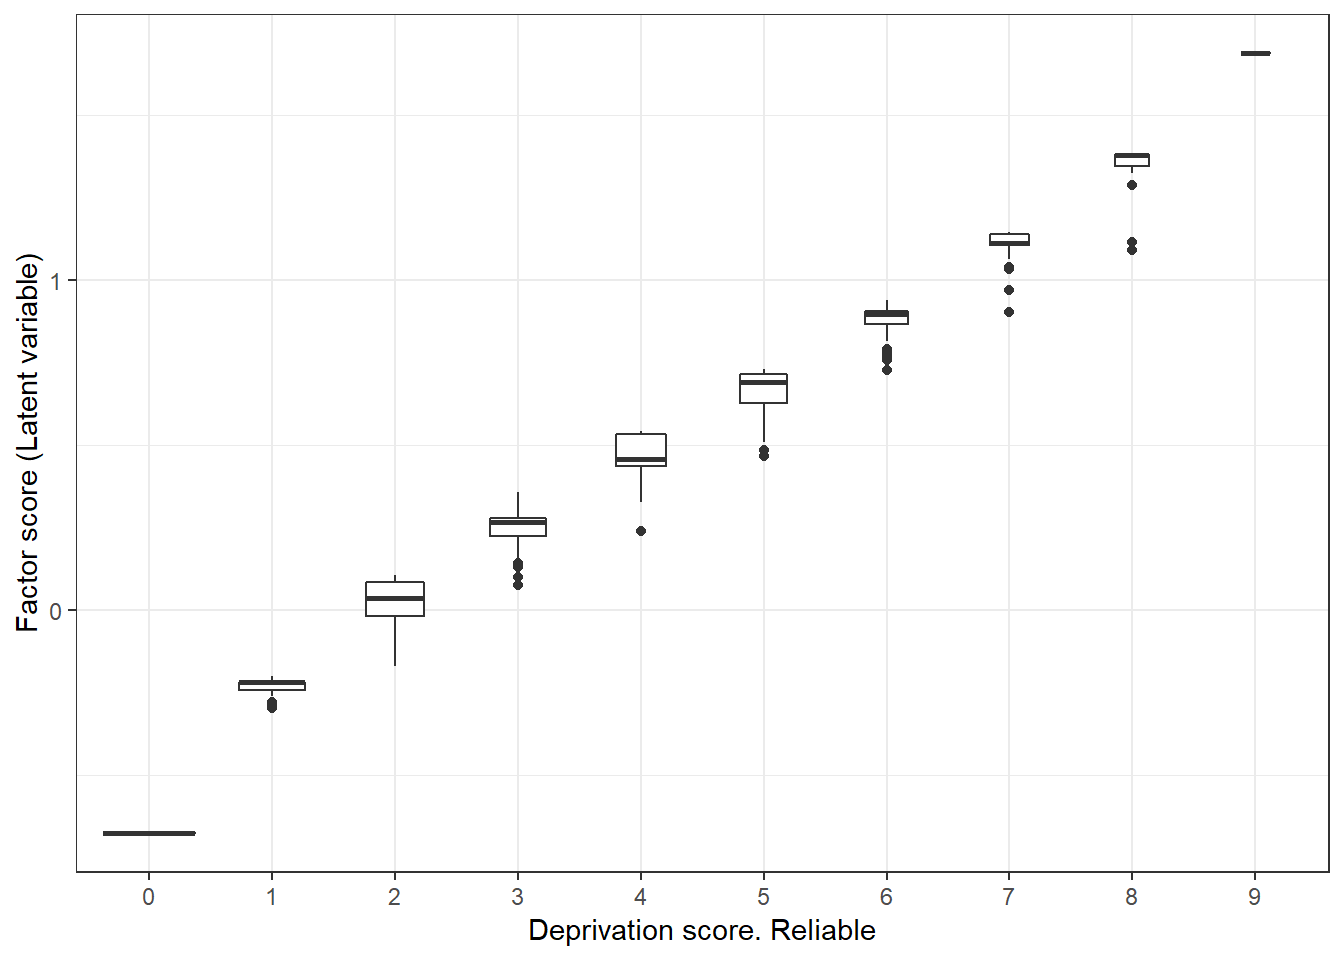
\includegraphics{PM_Book_files/figure-latex/fsdesrel-1.png}
\caption{\label{fig:fsdesrel}Relationship between the deprivation score (x1-x9) and the latent variable score. We appreciate the narrowness of the box plots, indicating good group separation.}
\end{figure}

\begin{Shaded}
\begin{Highlighting}[]
\NormalTok{g <-}\StringTok{ }\KeywordTok{ggplot}\NormalTok{(Rel_MD_}\DecValTok{1}\NormalTok{, }\KeywordTok{aes}\NormalTok{(}\KeywordTok{as.factor}\NormalTok{(ds_ur), hur))}
\NormalTok{g }\OperatorTok{+}\StringTok{ }\KeywordTok{geom_boxplot}\NormalTok{(}\DataTypeTok{varwidth=}\NormalTok{T) }\OperatorTok{+}\StringTok{ }
\StringTok{    }\KeywordTok{labs}\NormalTok{(}\DataTypeTok{x=}\StringTok{"Deprivation score. Unreliable"}\NormalTok{,}
         \DataTypeTok{y=}\StringTok{"Factor score (Latent variable)"}\NormalTok{) }\OperatorTok{+}\StringTok{ }\KeywordTok{theme_bw}\NormalTok{()}
\end{Highlighting}
\end{Shaded}

\begin{figure}
\centering
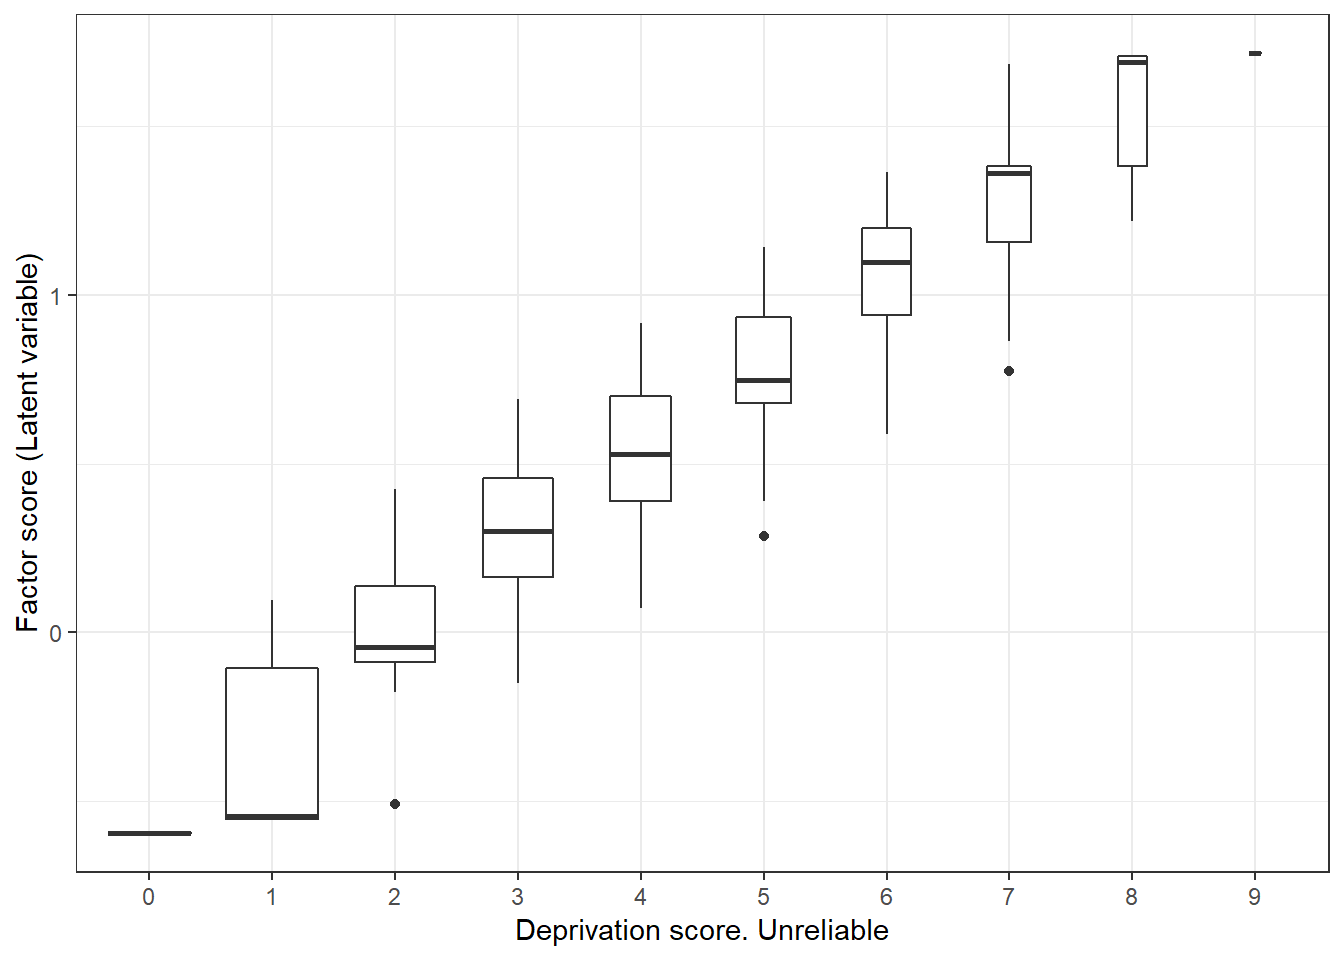
\includegraphics{PM_Book_files/figure-latex/fsdesunrel-1.png}
\caption{\label{fig:fsdesunrel}Relationship between the deprivation score (x10, x11 and x3-x9) and the latent variable score. There is more variability in this case indicating poor group separation.}
\end{figure}

\hypertarget{item-level-reliability}{%
\section{Item-level reliability}\label{item-level-reliability}}

Overall reliability is an excellent summary of the quality of an index in that it tells the homogeneity of our scale and its capacity to produce consistent population rankings. In section \emph{ref} we showed that including some uncorrelated items lead to a reduction of reliability and that this has negative implication for consistency across measurements. This section focuses on item reliability, i.e.~how specific items contribute positively or negatively to reliability.

Section \emph{ref} reviewed Item Response Theory (IRT), which is a theory of the properties of indicators by putting forward the concepts of discrimination and severity. The standard IRT modelling assummes that scales are unidimensional in that indicators are manifest of a latent trait. However, in parallel to the development of CFA, IRT modelling has incorporated multidimensional models. HOwever, as long as a scale is homogeneous, the bias from a multidimensional IRT and the unidimensional one should not dramatically change our conclusions about the reliability of the items.

To illustrate IRT modelling, we will work with the same data set, which we know that results in a highly homogeneous scale. We will use the data ``Rel\_MD\_1'' and the R-package \texttt{ltm} which fits different kinds of IRT models. The \texttt{ltm()} function fits one, two and three-parameter IRT models. Below we fit a two-parameter IRT model simply by adding the \texttt{z1} option so we allow the model to have different slopes, i.e.~Two-parameter IRT model. The output shows the difficulty and discrimination coefficients. The difficulty represents the severity of the deprivation on the latent trait. For example, item x1 is less severe than item x3. The second column \texttt{Dscrmn} displays the values of the discrimination parameters. All the items have values \(>.9\) which is above the suggested threshold by Guio et al. (\protect\hyperlink{ref-Guio2016}{2016}) and Nájera (\protect\hyperlink{ref-Najera2018}{2018}).

\begin{Shaded}
\begin{Highlighting}[]
\KeywordTok{library}\NormalTok{(ltm)}
\NormalTok{rel_irt<-}\KeywordTok{ltm}\NormalTok{(Rel_MD_}\DecValTok{1}\NormalTok{[,}\KeywordTok{c}\NormalTok{(}\DecValTok{1}\OperatorTok{:}\DecValTok{9}\NormalTok{)] }\OperatorTok{~}\StringTok{ }\NormalTok{z1)}
\NormalTok{rel_irt}
\end{Highlighting}
\end{Shaded}

\begin{verbatim}
## 
## Call:
## ltm(formula = Rel_MD_1[, c(1:9)] ~ z1)
## 
## Coefficients:
##     Dffclt  Dscrmn
## x1   0.023   2.290
## x2   0.702   2.183
## x3   1.258   2.198
## x4   0.053   2.306
## x5   0.698   2.368
## x6   1.297   2.154
## x7   0.160   2.541
## x8   0.802   2.547
## x9   1.236   2.477
## 
## Log.Lik: -20132.92
\end{verbatim}

Before checking the estimation with Mplus, we will check what will happen if we include our unreliable items. Items x1 and x2 are replaced by items V1 and V2. As expected the discrimination values are unacceptably low as well as the severity values which are (\(\geq3\)) standard deviations.

\begin{Shaded}
\begin{Highlighting}[]
\KeywordTok{head}\NormalTok{(Rel_MD_}\DecValTok{1}\NormalTok{[,}\KeywordTok{c}\NormalTok{(}\DecValTok{3}\OperatorTok{:}\DecValTok{11}\NormalTok{)])}
\end{Highlighting}
\end{Shaded}

\begin{verbatim}
##   x3 x4 x5 x6 x7 x8 x9 x10 x11
## 1  1  1  0  0  0  0  0   0   0
## 2  0  0  0  0  0  0  0   0   0
## 3  0  1  0  0  0  0  0   0   0
## 4  0  0  0  0  1  0  0   0   0
## 5  0  0  0  0  0  0  0   1   1
## 6  0  0  0  0  0  0  0   0   0
\end{verbatim}

\begin{Shaded}
\begin{Highlighting}[]
\NormalTok{rel_irt_}\DecValTok{2}\NormalTok{<-}\KeywordTok{ltm}\NormalTok{(Rel_MD_}\DecValTok{1}\NormalTok{[,}\KeywordTok{c}\NormalTok{(}\DecValTok{3}\OperatorTok{:}\DecValTok{11}\NormalTok{)] }\OperatorTok{~}\StringTok{ }\NormalTok{z1)}
\NormalTok{rel_irt_}\DecValTok{2}
\end{Highlighting}
\end{Shaded}

\begin{verbatim}
## 
## Call:
## ltm(formula = Rel_MD_1[, c(3:11)] ~ z1)
## 
## Coefficients:
##      Dffclt  Dscrmn
## x3    1.426   1.651
## x4    0.053   2.371
## x5    0.689   2.488
## x6    1.279   2.245
## x7    0.157   2.817
## x8    0.780   2.840
## x9    1.193   2.804
## x10   5.142   0.133
## x11   4.882   0.135
## 
## Log.Lik: -21740.2
\end{verbatim}

Similarly we can fit the model using items (x1-x9) in Mplus using the package ``mplusAutomation'' by creating an object with \texttt{mplusObject()}.

\begin{Shaded}
\begin{Highlighting}[]
\NormalTok{test <-}\StringTok{ }\KeywordTok{mplusObject}\NormalTok{(}
\DataTypeTok{TITLE =} \StringTok{"IRT model;"}\NormalTok{,}
   \DataTypeTok{VARIABLE =} \StringTok{"}
\StringTok{     NAMES = x1-x9 resources educ_yr occupation hh_size class;}
\StringTok{     CATEGORICAL = x1-x9;}
\StringTok{     USEVARIABLES = x1-x9;"}\NormalTok{,}
   \DataTypeTok{ANALYSIS =} \StringTok{"ESTIMATOR = ml;}
\StringTok{              PROCESS = 4;"}\NormalTok{,}

\DataTypeTok{MODEL =} \StringTok{"h by x1* x2-x9;}
\StringTok{         h@1;"}\NormalTok{)}
\end{Highlighting}
\end{Shaded}

Then the model is fitted using \texttt{mplusModeler()}. We will name our Mplus script as ``rel\_IRT\_1.inp'' and we will be using the same data as before (``Rel\_MD\_data\_1\_1.dat'') and we request Mplus to run the model directly from the script with (\texttt{run}).

\begin{Shaded}
\begin{Highlighting}[]
\NormalTok{res <-}\StringTok{ }\KeywordTok{mplusModeler}\NormalTok{(test, }\DataTypeTok{modelout =} \StringTok{"rel_IRT_1.inp"}\NormalTok{, }
                    \DataTypeTok{writeData =} \StringTok{"never"}\NormalTok{, }\DataTypeTok{hashfilename =} \OtherTok{FALSE}\NormalTok{, }
                    \DataTypeTok{dataout=}\StringTok{"Rel_MD_data_1_1.dat"}\NormalTok{, }\DataTypeTok{run =}\NormalTok{ 1L)}
\end{Highlighting}
\end{Shaded}

Now we read the result of our model with \texttt{readModels()}.

\begin{Shaded}
\begin{Highlighting}[]
\NormalTok{REL_IRT_}\DecValTok{1}\NormalTok{<-}\KeywordTok{readModels}\NormalTok{(}\DataTypeTok{filefilter =}\StringTok{"rel_IRT_1"}\NormalTok{)}
\end{Highlighting}
\end{Shaded}

The \texttt{readModels()} does an excellent job in extracting and ordering the Mplus output. It puts all the relevant result in lists. We can see that the Mplus estimates are very similar to those obtained from the \texttt{ltm} package.

\begin{Shaded}
\begin{Highlighting}[]
\NormalTok{rel_irt<-REL_IRT_}\DecValTok{1}\OperatorTok{$}\NormalTok{parameters}\OperatorTok{$}\NormalTok{irt.parameterization}
\NormalTok{rel_irt<-rel_irt[}\DecValTok{1}\OperatorTok{:}\DecValTok{18}\NormalTok{,]}
\NormalTok{rel_irt<-}\KeywordTok{data.frame}\NormalTok{(}\DataTypeTok{a=}\NormalTok{rel_irt}\OperatorTok{$}\NormalTok{est[}\DecValTok{1}\OperatorTok{:}\DecValTok{9}\NormalTok{],}\DataTypeTok{b=}\NormalTok{rel_irt}\OperatorTok{$}\NormalTok{est[}\DecValTok{10}\OperatorTok{:}\DecValTok{18}\NormalTok{])}
\NormalTok{rel_irt}
\end{Highlighting}
\end{Shaded}

\begin{verbatim}
##       a     b
## 1 2.290 0.024
## 2 2.192 0.700
## 3 2.207 1.254
## 4 2.312 0.054
## 5 2.383 0.696
## 6 2.172 1.291
## 7 2.548 0.161
## 8 2.561 0.800
## 9 2.498 1.231
\end{verbatim}

\hypertarget{multidimensional-item-reliability-evaluation}{%
\section{Multidimensional item-reliability evaluation}\label{multidimensional-item-reliability-evaluation}}

A multidimensional IRT model is just a CFA model with categorical indicators. One way to assess the item-level reliability is by looking at the loadings from a CFA model. We can fit a higher-order factor model (equivalent to the bi-factor model above) to assess the value of the loadings and and look at the \(R^2\) values of each indicator (which is just \(\lambda{hj}^2\)). \(R^2\leq.25\) are equivalent to \(\lambda{hj}^2\leq.5\), which are often used as cut offs of unacceptably low loadings. We see that all these items are highly reliable not only with regard the higher order factor but also in terms of each dimension, measured by each factor loading.

\begin{Shaded}
\begin{Highlighting}[]
\NormalTok{ MD_model <-}\StringTok{ ' f1  =~ x1 + x2 + x3}
\StringTok{              f2 =~ x4 + x5 + x6}
\StringTok{              f3   =~ x7 + x8 + x9}
\StringTok{                h =~ f1 + f2 + f3}
\StringTok{ '}

\NormalTok{fit <-}\StringTok{ }\KeywordTok{sem}\NormalTok{(MD_model, }\DataTypeTok{data =}\NormalTok{ Rel_MD_}\DecValTok{1}\NormalTok{,}
           \DataTypeTok{ordered=}\KeywordTok{c}\NormalTok{(}\StringTok{"x1"}\NormalTok{,}\StringTok{"x2"}\NormalTok{,}\StringTok{"x3"}\NormalTok{,}\StringTok{"x4"}\NormalTok{,}\StringTok{"x5"}\NormalTok{,}
                     \StringTok{"x6"}\NormalTok{,}\StringTok{"x7"}\NormalTok{,}\StringTok{"x8"}\NormalTok{,}\StringTok{"x9"}\NormalTok{))}
\KeywordTok{inspect}\NormalTok{(fit,}\DataTypeTok{what=}\StringTok{"std"}\NormalTok{)}\OperatorTok{$}\NormalTok{lambda}
\end{Highlighting}
\end{Shaded}

\begin{verbatim}
##       f1    f2    f3 h
## x1 0.924 0.000 0.000 0
## x2 0.888 0.000 0.000 0
## x3 0.873 0.000 0.000 0
## x4 0.000 0.929 0.000 0
## x5 0.000 0.917 0.000 0
## x6 0.000 0.866 0.000 0
## x7 0.000 0.000 0.947 0
## x8 0.000 0.000 0.916 0
## x9 0.000 0.000 0.894 0
\end{verbatim}

\hypertarget{item-reliability-and-monotonicity}{%
\subsection{Item-reliability and monotonicity}\label{item-reliability-and-monotonicity}}

Low loadings are an indication that the indicator is not a manifest variable of the underlying construct. That is, that changes in poverty do not mirror changes in deprivation. Section\textasciitilde{}\ref{} suggested that there is a relationship between item-reliability and the monotonicity axiom. Nájera (\protect\hyperlink{ref-NajeraForthcoming}{n.d.}) shows that indeed low loadings approximately \(\leq.5\) lead to violations of the strong monotonicity axiom, i.e.~a reduction in poverty does not reflect an improvement in the achievement matrix. Weak monotonicity is violated when an improvement in poverty results in an increase of deprivation, this would happen when the factor loadings are negative, for example.

We will fit a higher order model using again the unreliable items (x10 and x11) instead of x1 and x2. Of course, it is possible to use either the loadings of the \(R^2\) values (these can be obtained with the \texttt{summary()} function. We see again, as in the IRT analysis that both items have unacceptably low values. These items should be dropped from the scale as it inclusion introduces noise to our measure. That would imply dropping the first dimension in the absence of alternative indicators.

\begin{Shaded}
\begin{Highlighting}[]
\NormalTok{ MD_model <-}\StringTok{ ' f1  =~ x10 + x11 + x3}
\StringTok{              f2 =~ x4 + x5 + x6}
\StringTok{              f3   =~ x7 + x8 + x9}
\StringTok{                h =~ f1 + f2 + f3}
\StringTok{ '}

\NormalTok{fit <-}\StringTok{ }\KeywordTok{sem}\NormalTok{(MD_model, }\DataTypeTok{data =}\NormalTok{ Rel_MD_}\DecValTok{1}\NormalTok{,}
           \DataTypeTok{ordered=}\KeywordTok{c}\NormalTok{(}\StringTok{"x10"}\NormalTok{,}\StringTok{"x11"}\NormalTok{,}\StringTok{"x3"}\NormalTok{,}\StringTok{"x4"}\NormalTok{,}\StringTok{"x5"}\NormalTok{,}
                      \StringTok{"x6"}\NormalTok{,}\StringTok{"x7"}\NormalTok{,}\StringTok{"x8"}\NormalTok{,}\StringTok{"x9"}\NormalTok{))}
\end{Highlighting}
\end{Shaded}

\begin{verbatim}
## Warning in lav_object_post_check(object): lavaan WARNING: some estimated ov
## variances are negative
\end{verbatim}

\begin{Shaded}
\begin{Highlighting}[]
\KeywordTok{inspect}\NormalTok{(fit,}\DataTypeTok{what=}\StringTok{"std"}\NormalTok{)}\OperatorTok{$}\NormalTok{lambda}
\end{Highlighting}
\end{Shaded}

\begin{verbatim}
##        f1    f2    f3 h
## x10 0.114 0.000 0.000 0
## x11 0.116 0.000 0.000 0
## x3  1.036 0.000 0.000 0
## x4  0.000 0.924 0.000 0
## x5  0.000 0.920 0.000 0
## x6  0.000 0.868 0.000 0
## x7  0.000 0.000 0.947 0
## x8  0.000 0.000 0.914 0
## x9  0.000 0.000 0.898 0
\end{verbatim}

\hypertarget{real-data-example}{%
\section{Real data example}\label{real-data-example}}

We will use the Mexican data set ``Mex\_pobreza\_14.dat''. This data set contains a subset of the deprivation indicators utlised to measure multidimensional poverty in Mexico. The official measure has two domains: income and social rights. The social rights domain has five dimensions: essential services, housing, food deprivation, social security and education. Some of this dimensions are measured with few indicators, like education and social security. This poses limitations to fit an identified model. Hence, we will use a reduced version of the model comprising three dimensions: essential services, housing and food deprivation.

The Mexican poverty data comes from a nationally representative complex survey. We will use the package ``survey'' (Lumley, \protect\hyperlink{ref-Lumley2016}{2016}). This is a comprehensive R-package to analyse survey data. We strongly advice readers to check Lumley (\protect\hyperlink{ref-Lumley2011}{2011}) book on complex surveys to get a depth insight on complex sampling and the use of Lumley's excellent package. To produce design deprivation rates estimates for each of the 14 items we need to specify few things. First we need to identify the sampling weights and the primary sampling units (PSU). The (\texttt{options()}) function is to prevent errors as sometimes there is one household per PSU. Once we have set up the sampling design we can estimate the deprivation rates with the \texttt{svymean()} function -we round the percentages for simplicity-. We can see than deprivation in the housing dimension items is rather low. Essential services present higher deprivation rates but electricity is very low. We see that the food deprivation items have the higher rates on average.

\begin{Shaded}
\begin{Highlighting}[]
\KeywordTok{library}\NormalTok{(haven)}
\NormalTok{Mex_D<-}\KeywordTok{read_dta}\NormalTok{(}\StringTok{"pobreza_14.dta"}\NormalTok{)}

\NormalTok{cols <-}\StringTok{ }\KeywordTok{c}\NormalTok{(}\StringTok{"icv_muros"}\NormalTok{, }\StringTok{"icv_techos"}\NormalTok{, }\StringTok{"icv_pisos"}\NormalTok{, }\StringTok{"icv_hac"}\NormalTok{,}
          \StringTok{"isb_agua"}\NormalTok{,}\StringTok{"isb_dren"}\NormalTok{, }\StringTok{"isb_luz"}\NormalTok{, }\StringTok{"isb_combus"}\NormalTok{,}
          \StringTok{"ic_sbv"}\NormalTok{, }\StringTok{"ia_1ad"}\NormalTok{, }\StringTok{"ia_2ad"}\NormalTok{, }\StringTok{"ia_3ad"}\NormalTok{, }\StringTok{"ia_4ad"}\NormalTok{, }
          \StringTok{"ia_5ad"}\NormalTok{,  }\StringTok{"ia_6ad"}\NormalTok{)}

\KeywordTok{library}\NormalTok{(survey)}
\KeywordTok{options}\NormalTok{(}\DataTypeTok{scipen=}\DecValTok{999}\NormalTok{, }\DataTypeTok{survey.lonely.psu=}\StringTok{"adjust"}\NormalTok{)}
\NormalTok{des <-}\StringTok{ }\KeywordTok{svydesign}\NormalTok{(}\DataTypeTok{data=}\NormalTok{Mex_D, }\DataTypeTok{id=}\OperatorTok{~}\DecValTok{1}\NormalTok{, }\DataTypeTok{CLUSTER=}\OperatorTok{~}\NormalTok{psu, }\DataTypeTok{weights=}\OperatorTok{~}\NormalTok{weight)}
\NormalTok{propr <-}\StringTok{ }\KeywordTok{data.frame}\NormalTok{(}\KeywordTok{svymean}\NormalTok{(Mex_D[, cols],des,}\DataTypeTok{na.rm=}\NormalTok{T))}
\NormalTok{propr <-}\StringTok{ }\KeywordTok{round}\NormalTok{(propr}\OperatorTok{*}\DecValTok{100}\NormalTok{,}\DecValTok{1}\NormalTok{)}
\NormalTok{propr}
\end{Highlighting}
\end{Shaded}

\begin{verbatim}
##            mean  SE
## icv_muros   1.7 0.1
## icv_techos  1.6 0.1
## icv_pisos   3.0 0.1
## icv_hac     5.6 0.1
## isb_agua    7.7 0.1
## isb_dren    7.5 0.1
## isb_luz     0.8 0.0
## isb_combus 12.0 0.2
## ic_sbv     19.6 0.2
## ia_1ad     33.3 0.3
## ia_2ad     15.9 0.2
## ia_3ad     24.9 0.2
## ia_4ad     14.0 0.2
## ia_5ad     16.4 0.2
## ia_6ad     12.3 0.2
\end{verbatim}

Now the we are familiarised with the 14 deprivation indicators we can proceed to estimate the reliability statistics. We will fit the model in Mplus as we will incorporate the survey design in the estimation of the parameters -it is possible to do so with the \texttt{lavaan.survey()} too-. We first create our Mplus script (rel\_CFA\_mex.inp) to fit the bi-factor model. Following the theoretical model for this data, the model has three dimensions (housing (f1), essential services (f2) and food deprivaton (f3)) and one higher-order factor (h). Once the model has been fitted we will store the output in the object called \texttt{REL\textbackslash{}\_CFA\textbackslash{}\_mex}.

\begin{Shaded}
\begin{Highlighting}[]
\NormalTok{test <-}\StringTok{ }\KeywordTok{mplusObject}\NormalTok{(}
\DataTypeTok{TITLE =} \StringTok{"Bi-factor model CFA;"}\NormalTok{,}
   \DataTypeTok{VARIABLE =} \StringTok{"}
\StringTok{     NAMES = proyecto folioviv foliohog icv_muros icv_techos }
\StringTok{             icv_pisos icv_hac isb_agua isb_dren isb_luz isb_combus}
\StringTok{             ic_sbv ia_1ad ia_2ad ia_3ad ia_4ad ia_5ad ia_6ad}
\StringTok{             ia_7men ia_8men ia_9men ia_10men ia_11men ia_12men }
\StringTok{             tv_dep radio_dep fridge_dep}
\StringTok{             washingmach_dep compu_dep inter_dep psu weight}
\StringTok{             rururb tot_integ durables educ_hh; }
\StringTok{MISSING=.;}
\StringTok{     CATEGORICAL = icv_muros icv_techos icv_pisos icv_hac isb_agua}
\StringTok{                   isb_dren isb_luz isb_combus  ia_1ad }
\StringTok{                   ia_2ad ia_3ad ia_4ad ia_5ad ia_6ad;}
\StringTok{     USEVARIABLES = icv_muros icv_techos icv_pisos icv_hac isb_agua}
\StringTok{                   isb_dren isb_luz isb_combus  ia_1ad }
\StringTok{                   ia_2ad ia_3ad ia_4ad ia_5ad ia_6ad;}

\StringTok{WEIGHT=weight;}
\StringTok{cluster = psu;"}\NormalTok{,}

   \DataTypeTok{ANALYSIS =} \StringTok{"TYPE = complex;}

\StringTok{ESTIMATOR = wlsmv;}
\StringTok{PROCESS = 4;"}\NormalTok{,}

\DataTypeTok{MODEL =} \StringTok{"f1 by icv_muros icv_techos icv_pisos icv_hac;}
\StringTok{  f2 by isb_agua}
\StringTok{        isb_dren isb_luz isb_combus;}
\StringTok{  f3 by ia_1ad ia_2ad ia_3ad ia_4ad ia_5ad ia_6ad;}
\StringTok{  h  by icv_muros icv_techos icv_pisos icv_hac isb_agua}
\StringTok{        isb_dren isb_luz isb_combus ia_1ad ia_2ad }
\StringTok{        ia_3ad ia_4ad ia_5ad ia_6ad;}
\StringTok{  F1 with F2@0;}
\StringTok{  F2 with F3@0;}
\StringTok{  F3 with F1@0;}
\StringTok{  h with f1@0;}
\StringTok{  h with f2@0;}
\StringTok{  h with f3@0;"}\NormalTok{,}

\DataTypeTok{OUTPUT =} \StringTok{"std stdyx;"}\NormalTok{)}

\KeywordTok{mplusModeler}\NormalTok{(test, }\DataTypeTok{modelout =} \StringTok{"rel_CFA_mex.inp"}\NormalTok{, }
                    \DataTypeTok{writeData =} \StringTok{"never"}\NormalTok{, }\DataTypeTok{hashfilename =} \OtherTok{FALSE}\NormalTok{, }
                    \DataTypeTok{dataout=}\StringTok{"Mex_pobreza_14.dat"}\NormalTok{, }\DataTypeTok{run =}\NormalTok{ 1L)}
\NormalTok{REL_CFA_mex<-}\KeywordTok{readModels}\NormalTok{(}\StringTok{"rel_CFA_mex.out"}\NormalTok{)}
\end{Highlighting}
\end{Shaded}

We then can estimate the overall reliability statistics; both \(\omega\) and \(\omega_h\)\footnote{Prior the estimation of the reliability statistics is vital to inspect the fit of the model as a poor model will not be useful to estimate omega. We will discuss in the next chapter (Validity) the meaning of these statistics. At this point we will focus on the fact that a poor model fit invariably leads to poor estimates of reliability. There is no point in estimating reliability of a scale that makes no sense at all. To assess the fit of the model we look at four statistics: \(\chi^2\), TLI, CFI and RMSEA. For this model the relative statistics of fit look fine and we have some certainties about the model we fit.}. The reliability of our measure is very high under both statistics and both are above the recommended thresholds (Nájera, \protect\hyperlink{ref-Najera2018}{2018}). To estimate the reliability measures we will use the same approach we followed in the previous section. First, we will obtain the factor loadings (f's and h) and the errors for each indicator. Then we we will take the square of the sum of the lambdas (f1, f2, f3 and h) and the error sum. \(\omega\) and \(\omega_h\) then can be calculated using formulas from equations \eqref{eq:omega} and @ref(eq:omegah\}).

The values of both \(\omega\) and \(\omega_h\) are high .97 and .81, respectively. These figures suggest that this multidimensional scale is homogeneous but has multidimensional features (\(\omega_h<\omega\)).

\begin{Shaded}
\begin{Highlighting}[]
\NormalTok{lambdas<-REL_CFA_mex}\OperatorTok{$}\NormalTok{parameters}\OperatorTok{$}\NormalTok{std.standardized[}\DecValTok{1}\OperatorTok{:}\DecValTok{28}\NormalTok{,}\DecValTok{1}\OperatorTok{:}\DecValTok{3}\NormalTok{]}
\NormalTok{error<-REL_CFA_mex}\OperatorTok{$}\NormalTok{parameters}\OperatorTok{$}\NormalTok{r2[}\DecValTok{6}\NormalTok{]}

\NormalTok{lambda_}\DecValTok{2}\NormalTok{<-}\KeywordTok{sum}\NormalTok{(lambdas[}\DecValTok{10}\OperatorTok{:}\DecValTok{28}\NormalTok{,}\DecValTok{3}\NormalTok{])}\OperatorTok{^}\DecValTok{2} \OperatorTok{+}\StringTok{ }\KeywordTok{sum}\NormalTok{(lambdas[}\DecValTok{1}\OperatorTok{:}\DecValTok{4}\NormalTok{,}\DecValTok{3}\NormalTok{])}\OperatorTok{^}\DecValTok{2} \OperatorTok{+}\StringTok{ }
\StringTok{          }\KeywordTok{sum}\NormalTok{(lambdas[}\DecValTok{5}\OperatorTok{:}\DecValTok{8}\NormalTok{,}\DecValTok{3}\NormalTok{])}\OperatorTok{^}\DecValTok{2} \OperatorTok{+}\StringTok{ }\KeywordTok{sum}\NormalTok{(lambdas[}\DecValTok{9}\OperatorTok{:}\DecValTok{14}\NormalTok{,}\DecValTok{3}\NormalTok{])}\OperatorTok{^}\DecValTok{2}
\NormalTok{error <-}\StringTok{ }\KeywordTok{sum}\NormalTok{(error)}

\NormalTok{omega_t <-}\StringTok{ }\NormalTok{lambda_}\DecValTok{2} \OperatorTok{/}\StringTok{ }\NormalTok{(lambda_}\DecValTok{2}\OperatorTok{+}\NormalTok{error)}
\NormalTok{omega_h <-}\StringTok{ }\KeywordTok{sum}\NormalTok{(lambdas[}\DecValTok{10}\OperatorTok{:}\DecValTok{28}\NormalTok{,}\DecValTok{3}\NormalTok{])}\OperatorTok{^}\DecValTok{2} \OperatorTok{/}\StringTok{ }\NormalTok{(lambda_}\DecValTok{2}\OperatorTok{+}\NormalTok{error)}

\NormalTok{omega_t}
\end{Highlighting}
\end{Shaded}

\begin{verbatim}
## [1] 0.9730641
\end{verbatim}

\begin{Shaded}
\begin{Highlighting}[]
\NormalTok{omega_h}
\end{Highlighting}
\end{Shaded}

\begin{verbatim}
## [1] 0.8058398
\end{verbatim}

\hypertarget{item-level-reliability-1}{%
\subsection{Item-level reliability}\label{item-level-reliability-1}}

Once we have assessed the overall reliability of the Mexican index, we can assess item-reliability by fitting a higher-order factor model and checking the value of the factor loadings. We just simply need to rewrite our model (rel\_CFA\_mex2.inp) to represent a structure were the dimensions load into the higher order factor. This is simply done by specifying that h is measured by the three dimensions (f1, f2 and f3).

\begin{Shaded}
\begin{Highlighting}[]
\NormalTok{test <-}\StringTok{ }\KeywordTok{mplusObject}\NormalTok{(}
\DataTypeTok{TITLE =} \StringTok{"CFA higher order model CFA;"}\NormalTok{,}
   \DataTypeTok{VARIABLE =} \StringTok{"}
\StringTok{     NAMES = proyecto folioviv foliohog icv_muros icv_techos }
\StringTok{             icv_pisos icv_hac isb_agua isb_dren isb_luz isb_combus}
\StringTok{             ic_sbv ia_1ad ia_2ad ia_3ad ia_4ad ia_5ad ia_6ad}
\StringTok{             ia_7men ia_8men ia_9men ia_10men ia_11men ia_12men }
\StringTok{             tv_dep radio_dep fridge_dep}
\StringTok{             washingmach_dep compu_dep inter_dep psu weight}
\StringTok{            rururb tot_integ; }
\StringTok{MISSING=.;}
\StringTok{     CATEGORICAL = icv_muros icv_techos icv_pisos icv_hac isb_agua}
\StringTok{                   isb_dren isb_luz isb_combus  ia_1ad }
\StringTok{                   ia_2ad ia_3ad ia_4ad ia_5ad ia_6ad;}
\StringTok{     USEVARIABLES = icv_muros icv_techos icv_pisos icv_hac isb_agua}
\StringTok{                   isb_dren isb_luz isb_combus  ia_1ad }
\StringTok{                   ia_2ad ia_3ad ia_4ad ia_5ad ia_6ad;}

\StringTok{WEIGHT=weight;}
\StringTok{cluster = psu;"}\NormalTok{,}

   \DataTypeTok{ANALYSIS =} \StringTok{"TYPE = complex;}

\StringTok{ESTIMATOR = wlsmv;}
\StringTok{PROCESS = 4;"}\NormalTok{,}

\DataTypeTok{MODEL =} \StringTok{"f1 by icv_muros icv_techos icv_pisos icv_hac;}
\StringTok{  f2 by isb_agua}
\StringTok{        isb_dren isb_luz isb_combus;}
\StringTok{  f3 by ia_1ad ia_2ad ia_3ad ia_4ad ia_5ad ia_6ad;}
\StringTok{  h by f1 f2 f3;"}\NormalTok{,}

\DataTypeTok{OUTPUT =} \StringTok{"std stdyx;"}\NormalTok{)}

\KeywordTok{mplusModeler}\NormalTok{(test, }\DataTypeTok{modelout =} \StringTok{"rel_CFA_mex2.inp"}\NormalTok{, }
                    \DataTypeTok{writeData =} \StringTok{"never"}\NormalTok{, }\DataTypeTok{hashfilename =} \OtherTok{FALSE}\NormalTok{, }
                    \DataTypeTok{dataout=}\StringTok{"Mex_pobreza_14.dat"}\NormalTok{, }\DataTypeTok{run =}\NormalTok{ 1L)}
\end{Highlighting}
\end{Shaded}

Once the model has been fitted we can request the standardised factor loadings and inspect its values using the \texttt{readModels()}. To facilitate our interpretation we can plot the standardised loadings (Figure \ref{fig:lamdamex}. We see that all the indicators have very high loadings and above the suggested threshold (\(\lambda_ij>.5\)). That means that these indicators discriminate well and are reliable manifests of each dimension. We see, nonetheless, that the indicators of the housing dimension tend to have low values. This could be an indication that these indicators are losing discriminatory power due to changes in living standards.

\begin{Shaded}
\begin{Highlighting}[]
\NormalTok{REL_CFA_mex2<-}\KeywordTok{readModels}\NormalTok{(}\StringTok{"rel_CFA_mex2.out"}\NormalTok{)}
\NormalTok{modelParams<-}\StringTok{ }\NormalTok{REL_CFA_mex2}\OperatorTok{$}\NormalTok{parameters}\OperatorTok{$}\NormalTok{std.standardized[}\DecValTok{1}\OperatorTok{:}\DecValTok{14}\NormalTok{,]}
\NormalTok{modelParams <-}\StringTok{ }\KeywordTok{subset}\NormalTok{(modelParams, }\DataTypeTok{select=}\KeywordTok{c}\NormalTok{(}\StringTok{"paramHeader"}\NormalTok{, }\StringTok{"param"}\NormalTok{, }\StringTok{"est"}\NormalTok{, }\StringTok{"se"}\NormalTok{))}
\end{Highlighting}
\end{Shaded}

\begin{Shaded}
\begin{Highlighting}[]
\KeywordTok{library}\NormalTok{(ggplot2)}
\NormalTok{limits <-}\StringTok{ }\KeywordTok{aes}\NormalTok{(}\DataTypeTok{ymax =}\NormalTok{ est }\OperatorTok{+}\StringTok{ }\NormalTok{se, }\DataTypeTok{ymin=}\NormalTok{est }\OperatorTok{-}\StringTok{ }\NormalTok{se)}
 \KeywordTok{ggplot}\NormalTok{(modelParams, }\KeywordTok{aes}\NormalTok{(}\DataTypeTok{x=}\NormalTok{param, }\DataTypeTok{y=}\NormalTok{est)) }\OperatorTok{+}\StringTok{ }\KeywordTok{geom_pointrange}\NormalTok{(limits) }\OperatorTok{+}\KeywordTok{scale_x_discrete}\NormalTok{(}\StringTok{""}\NormalTok{) }\OperatorTok{+}
\StringTok{   }\KeywordTok{geom_hline}\NormalTok{(}\DataTypeTok{yintercept=}\DecValTok{0}\NormalTok{, }\DataTypeTok{color=}\StringTok{"grey50"}\NormalTok{) }\OperatorTok{+}\StringTok{ }\KeywordTok{theme_bw}\NormalTok{() }\OperatorTok{+}\KeywordTok{ylab}\NormalTok{(}\StringTok{"Std Loading"}\NormalTok{) }\OperatorTok{+}\StringTok{ }\KeywordTok{coord_flip}\NormalTok{()}
\end{Highlighting}
\end{Shaded}

\begin{figure}
\centering
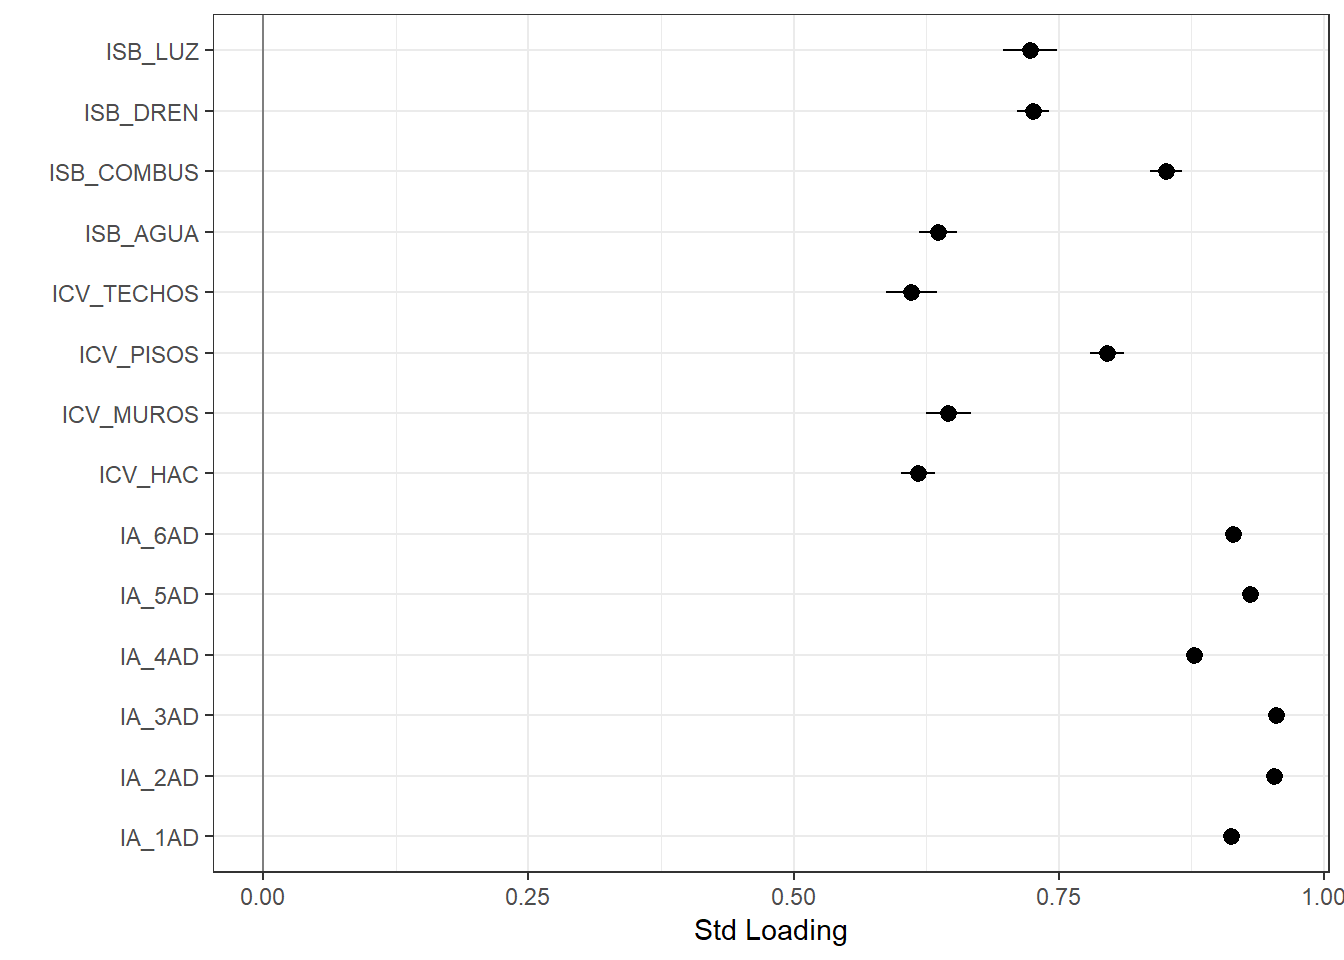
\includegraphics{PM_Book_files/figure-latex/lamdamex-1.png}
\caption{\label{fig:lamdamex}This plot shows the standardised values of the loadings for the 14 items.}
\end{figure}

\hypertarget{Chapter-4}{%
\chapter{Validity in poverty measurement}\label{Chapter-4}}

\textbf{Abstract}

This chapter focuses on the theory and implementation of validity. An intuitive explanation is provided about the relationship between reliability and validity and then the different definitions of validity are reviewed. The chapter then uses simulated data to illustrate how construct and criterion validity can be investigated using R and Mplus. The chapter finalised by looking at a real-data example.

\hypertarget{intuition-to-the-concept-of-validity}{%
\section{Intuition to the concept of validity}\label{intuition-to-the-concept-of-validity}}

We have seen so far that reliability is homogeneity in measurement and it means the capacity of a measure to reproduce the ranking of a population under changing conditions. Reliability, thus, will tell us whether the set of indicators will be useful to order individual's according to their latent scores which we presume reflect poverty. Therefore, reliability is a necessary condition for good measurement but not a sufficient one. We need to make sure that our indicators are effectively capturing poverty.

Imagine that we know the standards of living of two subject in a sample- one highly educated, wealthy and healthy and another with low education attainment, with a lot of debt and with systematic health problems. However, we find an unexpected result. The first subject is ranked lower than the second one, i.e.~is more likely to be poor than the second. Measurement theory tells us that our scale is reliable but invalid. That means that there is very little evidence to interpret our index in accordance with our theory and concept of poverty.

A valid measure is one that tells use the nature of what is being measured and its relationship with the index in question to its cause. Validity is a property that aims to assess the extent to which an index captures what we mean to measure. In other fields, one could ask someone the amount of sugary drink they had in a week. This information could be recoded using a questionnaire, for example. How can we validate this measurement? Well, we could follow someone everywhere and every time and take notes of their drinking behaviours. Then we could compare our measurement to hers to assess the precision of our instrument.

Can we follow the same strategy in poverty research? No, we cannot as we work with an unobserved construct. The history of the Standards for Educational and Psychological Testing summarises the conceptualisation of validation of constructs. The way forward has been an unified framework of validity which looks at the extent to which the existence evidence on a scale supports the intended interpretation of test scores for the proposed use (AERA, APA and NCME, \protect\hyperlink{ref-AERA2014}{2014}).

\hypertarget{theory-of-validity}{%
\section{Theory of validity}\label{theory-of-validity}}

Classical test theory (CTT) proposes that reliability is the maximum possible validity of a scale. Reliability is affected by both systematic and random error but systematic error only affect validity. How this is possible according to CTT? The observed score is just the combination of the true score plus error. Validity is a function of systematic error (i.e.~constant deviations from the construct of interest) and results in deviations from the construct of interest. That means that a scale can be reliable but always wrong because it always deviates from the target of interest. In CTT validity is formulated as follows:

\begin{equation}
\label{eq:validity1}
V = \frac{\sigma^2_{CI}} {\sigma^2_{observed}}
\end{equation}

The problem with this formulation is that it was little practical usage as the problem in question is knowing \(\sigma^2_{CI}\). The best approximation for this notion of validity consisted in focusin on the predictive capacity of a scale. Nonetheless, this approach to validity changed after the 1950s. Bandalos (\protect\hyperlink{ref-Bandalos2018}{2018}) provides and overview of how the \emph{standards} have both discussed and expanded the definition of validity over time. In the 1950s, criteria and predictive validity were the dominant approaches in both psychometrics and educational measurement literature. These two forms of validity focused on the correlation between the scale in question and a predictor of the phenomenon of interest. In our example, criterion validity would have shown that our scale had an inverse relationship with some observable attributes of the subject in the sample. Therefore, the scale would have been regarded as invalid from the perspective of criterion validity.

Criterion validity demands a clear theory about the causes and consequences of the phenomenon of interest. Townsend (\protect\hyperlink{ref-Townsend1979}{1979}) provides a good framework for such a purpose in that it provides a clear causal mechanism: command of resources, poverty and deprivation. Therefore, measures of command of resources (another latent construct) could be used to predict poverty. For example, in Townsend's theory there are five main types of resources. Drawing upon, Townsend (\protect\hyperlink{ref-Townsend1979}{1979}), criterion validity has been used in poverty measurement by Guio et al. (\protect\hyperlink{ref-Guio2012}{2012}) for the production of the European deprivation index and by Gordon (\protect\hyperlink{ref-Gordon2010}{2010}) in his proposal for the Mexican multidimensional measure. Similarly, Nandy \& Pomati (\protect\hyperlink{ref-Nandy2015}{2015}) used criterion validity to assess their proposed index for Benin.

The association of an index with a predictive criterion may be inadequate or infeasible in some circumstances. In practice, some scales are developed to target certain aspects of a construct, for example, in poverty research it could be acute poverty or housing and facilities deprivation. In other settings, policymakers or institutions might prioritise some aspects of poverty from a human rights perspective, for example. This consideration leads to content validity. In poverty measurement, perhaps the most emblematic recent example is the Mexican measure. Drawing upon the Mexican Constitution (1917), the National Social Development Law defined poverty in terms of social rights. Because the Mexican law represents the will of the people, this gives a content validity to the measure (Gordon, \protect\hyperlink{ref-Gordon2010}{2010}). This, nonetheless, does not means that the law will lead to a valid scale. It means that the one should assess validity in accordance to the definition, i.e.~examine whether the dimensions and indicators lead to a reliable and valid measure.

One critical question about content validity is about how does a researcher \textbf{knows} or \textbf{defines} the constituent parts of the phenomenon of interests. Most of the time these aspects come from theory. However, the use of mixed methods is a way to enhance the capacity of theorists to develop concepts and frameworks about the mechanisms through which such concepts interact. The use of different kinds of good data will enhance the theory that gives content to a concept. \textbf{Face validity} is a form of validation that comes mainly from qualitative work. One way to see face validity is thinking in terms of how transparent a test looks like for the participants of the measurement. In other words, how sensible a the contents of a poverty index seem to the poor and the not poor. There are several qualitative methods to assess face validity and the best implementation to date is the Poverty and Social Exclusion project implementation of the Consensual Method (Pantazis et al. (\protect\hyperlink{ref-Pantazis2006a}{2006}); Gordon (\protect\hyperlink{ref-Gordon2018}{2018})). This project follows the ideal work flow production of a poverty measure (see \ref{fig:idealwf}) in that the concept of poverty has a theory that defines it, the questionnaire is first calibrated with qualitative work (face validity), and then a survey questionnaire is developed with the explicit purpose of measuring multidimensional poverty.

However, as discussed in Figure \ref{fig:realwf}, in practice poverty researchers work with the data they already have and content validity is constrain and face validity is ignored. Furthermore, in many cases, criterion validity might not be available due to the fact that there is no a clear priority about the aspects of a concept that should be targeted in a measurement exercise. Furthermore, it might be the case that there is no clear predictor to conduct criterion validity. For example, when there is no agreement about the causes and correlate variables of poverty. Cronbach \& Meehl (\protect\hyperlink{ref-Cronbach1955}{1955}) put forward a third form of validity that suggest that the measurement of the construct should be useful to \emph{meaningfully} split groups. Whereas reliability guarantees certain ordering, construct validity focuses on the meaning of such ranking. Construct validity, at first, was seeing as the last resource but in the contemporary literature is no longer the case. Construct validity requires mounting evidence in favour that the scale does what is meant to do. Messick (\protect\hyperlink{ref-Messick1987}{1987}) argued that construct validity embraces almost all types of validity evidence. For him, all the available evidence on a scale adds to the latent rejection or continuity of a scale. AERA, APA and NCME (\protect\hyperlink{ref-AERA2014}{2014}) define validity as (p.14):

\begin{quote}
\emph{It is the degree to which all the accumulated evidence supports the intended interpretation of test scores for the proposed used.}
\end{quote}

This modern definition refers thus to the different types of evidence on the validity of a scale- criterion, predictive and content.

\hypertarget{methods-for-the-analysis-validity}{%
\section{Methods for the analysis validity}\label{methods-for-the-analysis-validity}}

\hypertarget{criterion-validity}{%
\subsection{Criterion validity}\label{criterion-validity}}

Criterion validation is characterised by the correlation between an index and an alternative measure on the cause or effects of the construct of interest. This book is not about the different explanations of poverty but requires an illustration of the importance of having a theory for validity. This requires a theoretical framework explaining the drivers and consequences of poverty as well as how these two relate with the concept of deprivation. There are several good books on theories of poverty (see for an overview of different sources)(Spicker et al., \protect\hyperlink{ref-Spicker2006}{2006}). Poverty theories are crudely classified into structural and individual-centred theories. Peter Townsend (\protect\hyperlink{ref-Townsend1993}{1993}) and Townsend (\protect\hyperlink{ref-Townsend1979}{1979}) provide and overview of these frameworks. To illustrate how a theory of poverty relates to validity we will draw upon Townsend's theory as it is one of the few frameworks that links an explanation of poverty with a cogent theory for its measurement.

Townsend predicts that the lack of command of different kinds of resources lead to deprivation. This means that poverty should be related with different expressions of command of resources such as position in the labour market, education attainment, social class, etc. Poverty leads to exclusion and is said to be a good predictor of ill-health, therefore, poverty should be correlated with a measure of health status too. This means that the type of the employment should be correlated with our index of poverty, for example.

Gordon (\protect\hyperlink{ref-Gordon2010}{2010}) proposes fitting a regression model to assess the extent to which the (reliable) indicators of a poverty measure correlate with a proxy measure of command of resources. He used income as a measure of resources given that the Mexican Income and Expenditure Survey lacked a validator (we reflected on the problem of data production for poverty measurement see section). He did fit a Generalized Linear Model (GLM) using a binary variable (income poverty. Poor=1 and Not poor=2) as a response variable and the deprivation indicators as predictors. The model was adjusted by urban/rural and household size. The expectation thus was to find relative risks ratios higher than 1 (\(\beta_i>1\)) as this is an indication that being deprived of a given item increased the chances of being classified as poor. In Gordon (\protect\hyperlink{ref-Gordon2010}{2010})'s example the validator is far from ideal but illustrates the idea of criterion validation. In figure \ref{fig:valgordon} it is proposed a slightly better validator such as the position in the labour market. International occupation scales that aim to measure socio-economic position could be useful for this purpose (Ganzeboom \& Treiman, \protect\hyperlink{ref-Ganzeboom1996}{1996}). There are other alternatives like using subjective indicators of well-being or self-assessments of health status as those used by Guio et al. (\protect\hyperlink{ref-Guio2012}{2012}).

\begin{figure}[H]

{\centering 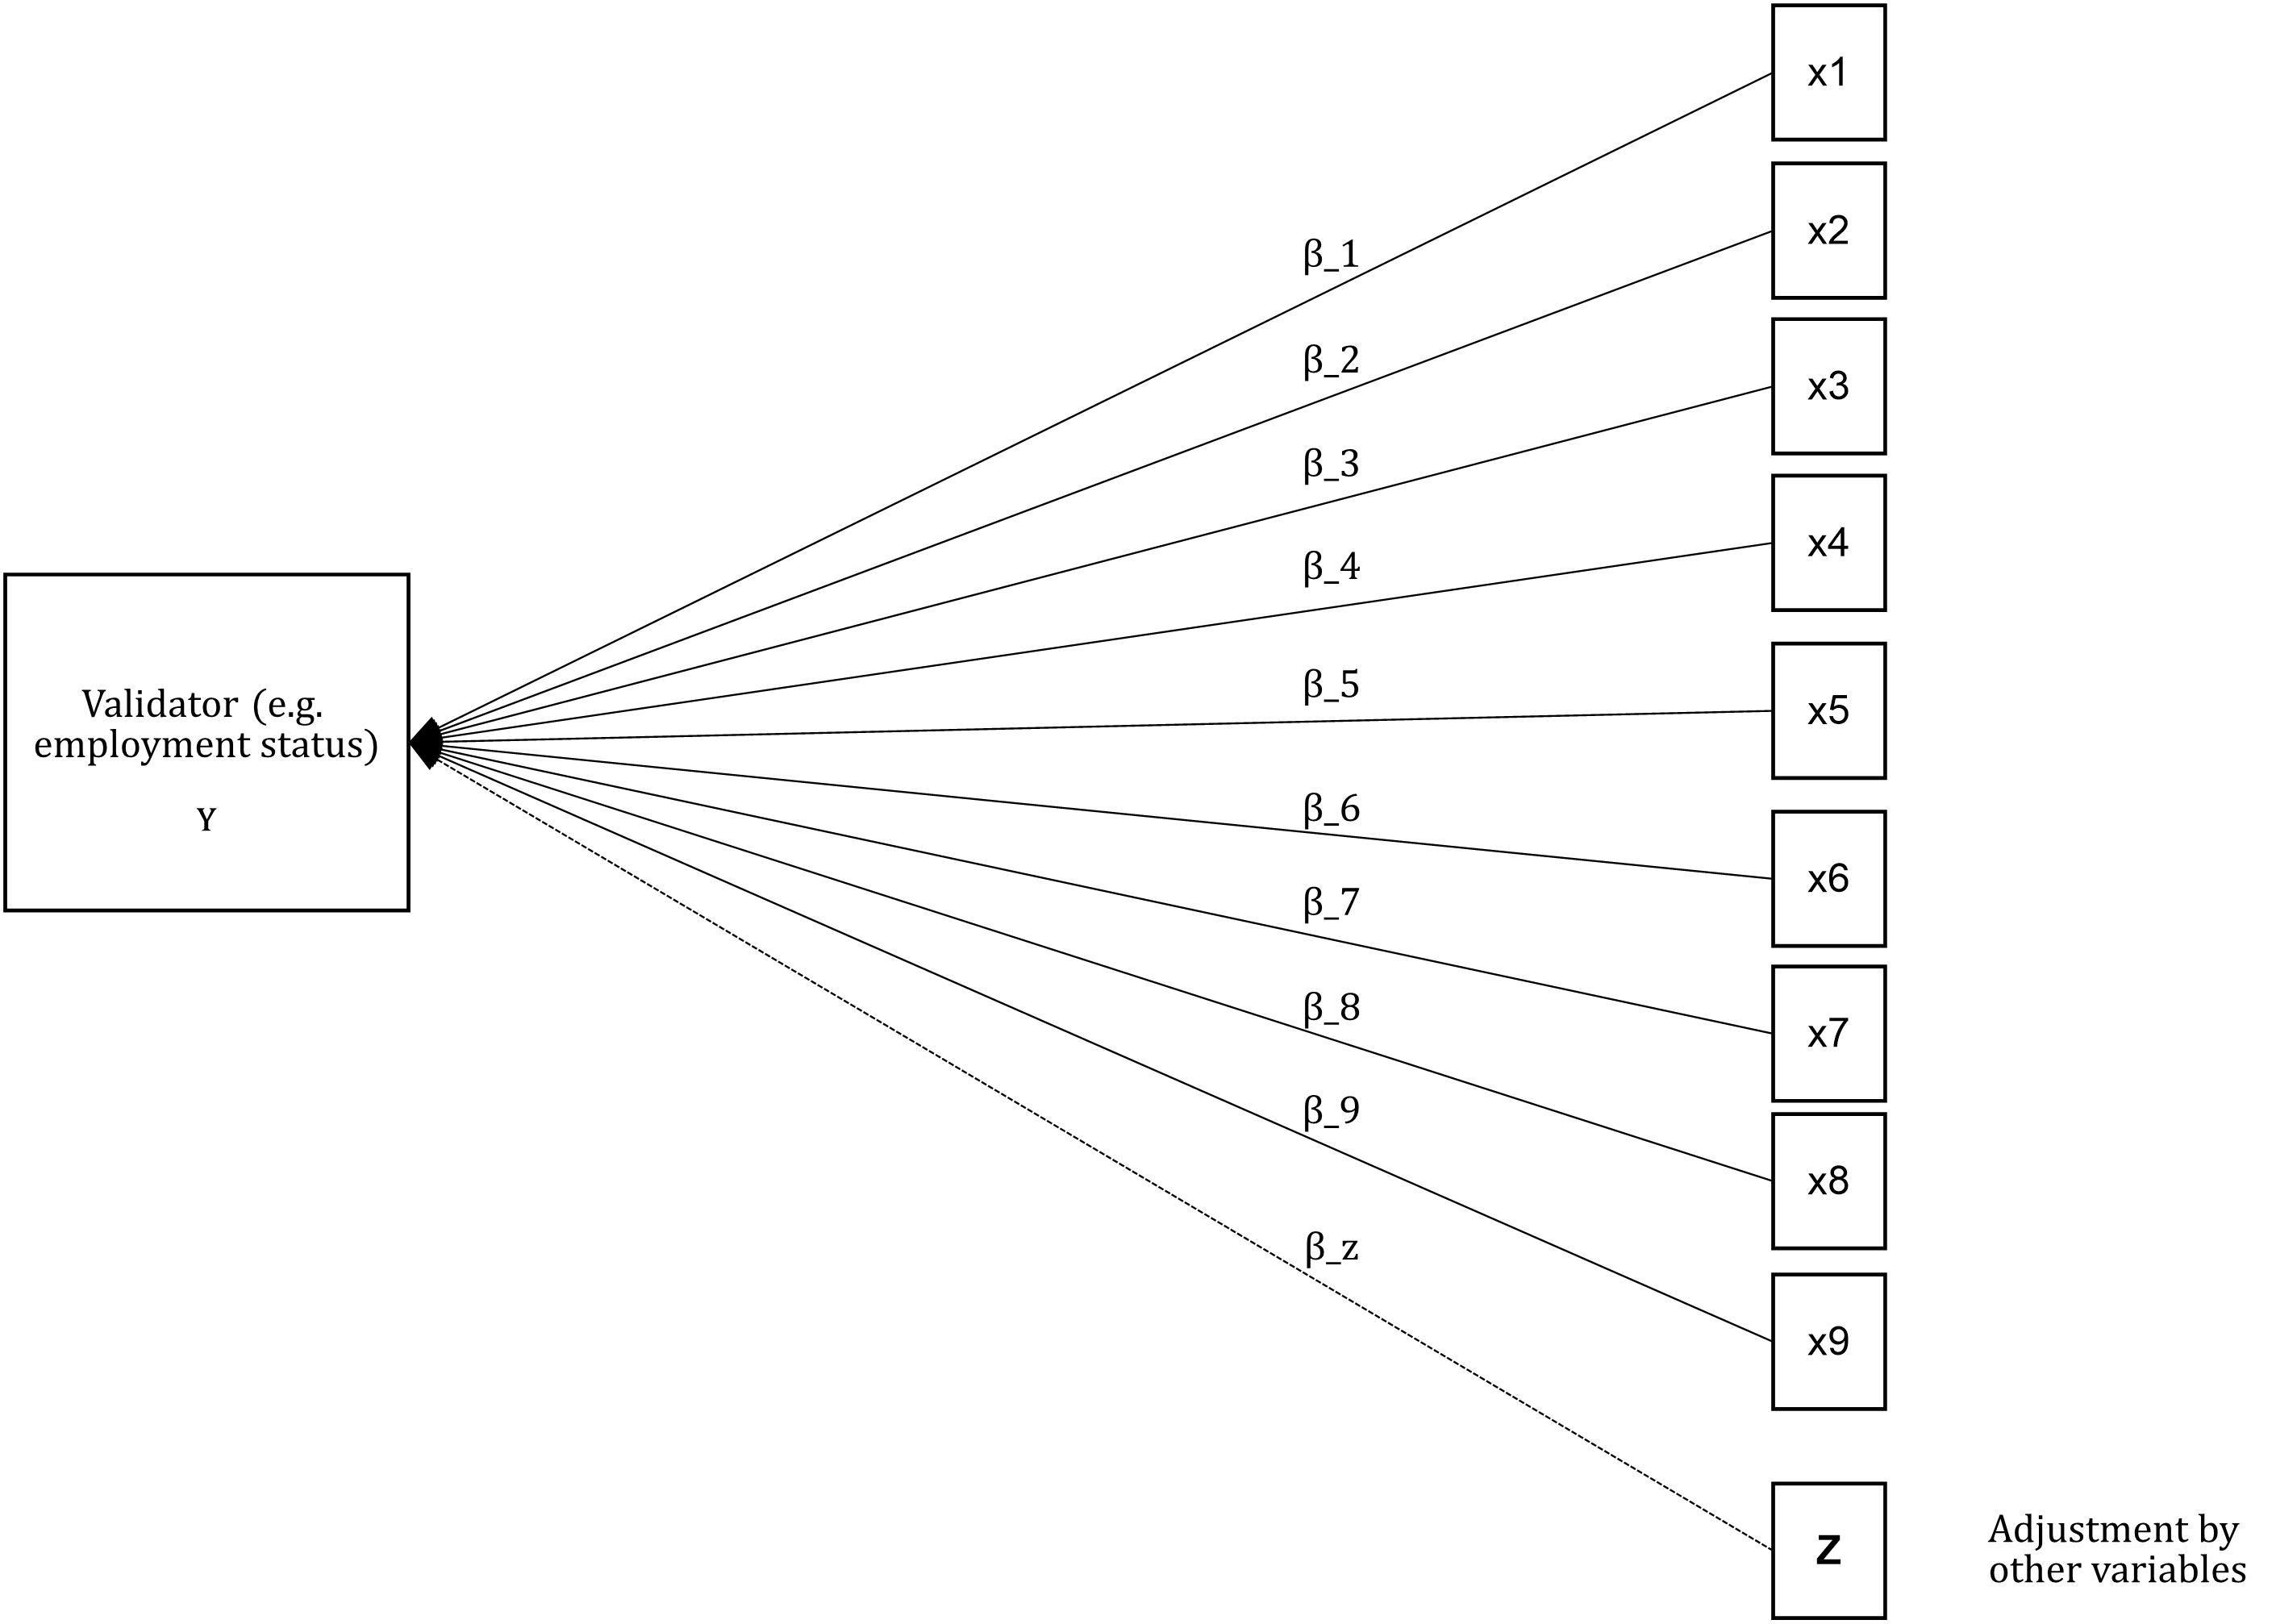
\includegraphics[width=\textwidth]{val_gordon} 

}

\caption{This is a visual representation of @Gordon2010 criterion validation. Here income poverty is replaced by a measure of socio-economic position like employment status.}\label{fig:valgordon}
\end{figure}

The advantage of using a unified framework such as measurement theory is that it is possible to further specifying a criterion validation model in terms of a Confirmatory Factor Model plus and explanatory model (Structural Equation Modelling, SEM). In the latent variable literature, these kind of models are known as MIMIC models or Multiple Indicator, Multiple Cause. Figure \ref{fig:valmimic} shows a visual representation of the criterion validation of the unidimensional model previously shown. In this case, there is a new path from the validator (Y) toward the latent variable. The model is adjusted by a series of covariates (Z). In this model the expectation would be to see that \(\beta_y\) to be associated with the factor (poverty) in a sensible way. If the metric of the factor (often standardised with mean zero and variance equal to one), tells that higher values denote higher severity, then we should expect that people with non-skilled jobs to be associated with positive factor values.

\begin{figure}[H]

{\centering 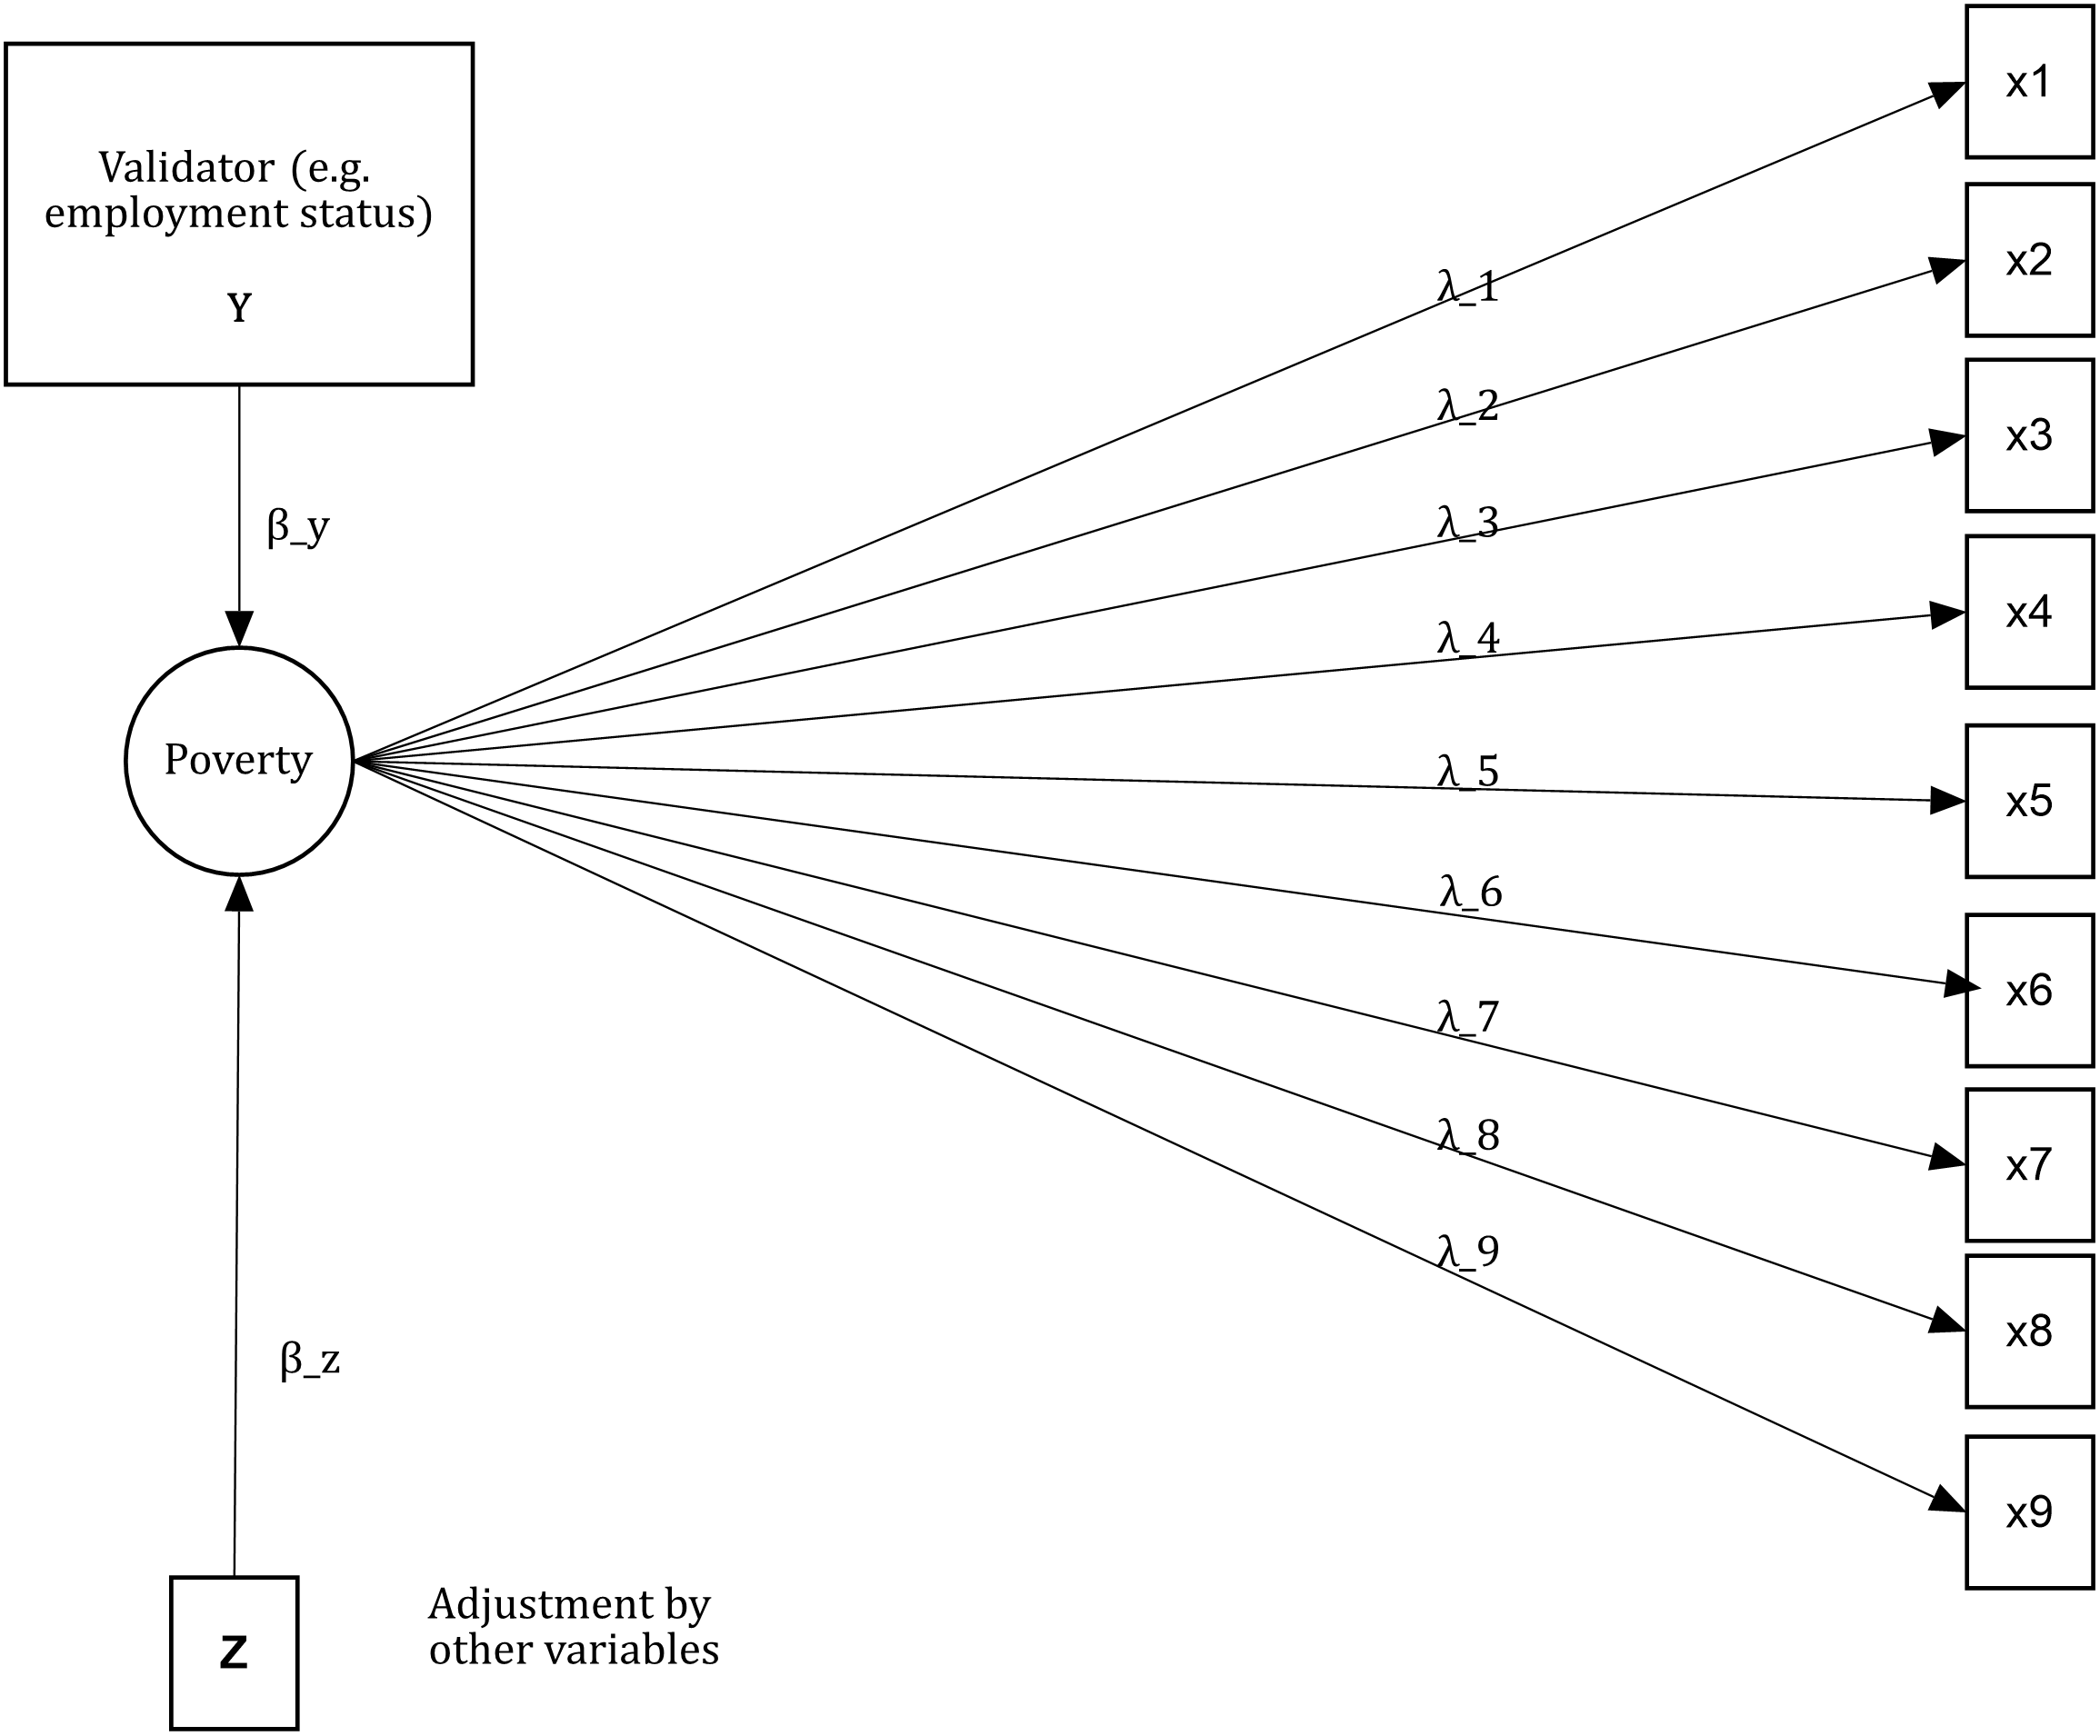
\includegraphics[width=\textwidth]{val_MIMIC} 

}

\caption{This is a visual representation of a MIMIC criterion validation of a unidimensional or null model}\label{fig:valmimic}
\end{figure}

We could easily extend this example of criterion validation for a simplified version of the Townsend model. Figure \ref{fig:valmdmimic} shows that poverty is predicted by a validator and some auxiliary variables (Z). The expectation is to find a predictive relationship between Y and the latent variable. The rest is just Townsend's measurement model of poverty. In this reduced version, only the two main dimensions are presented. In the next section is discussed that having just two dimensions leads to some identification issues for the empirical analysis.

\begin{figure}[H]

{\centering 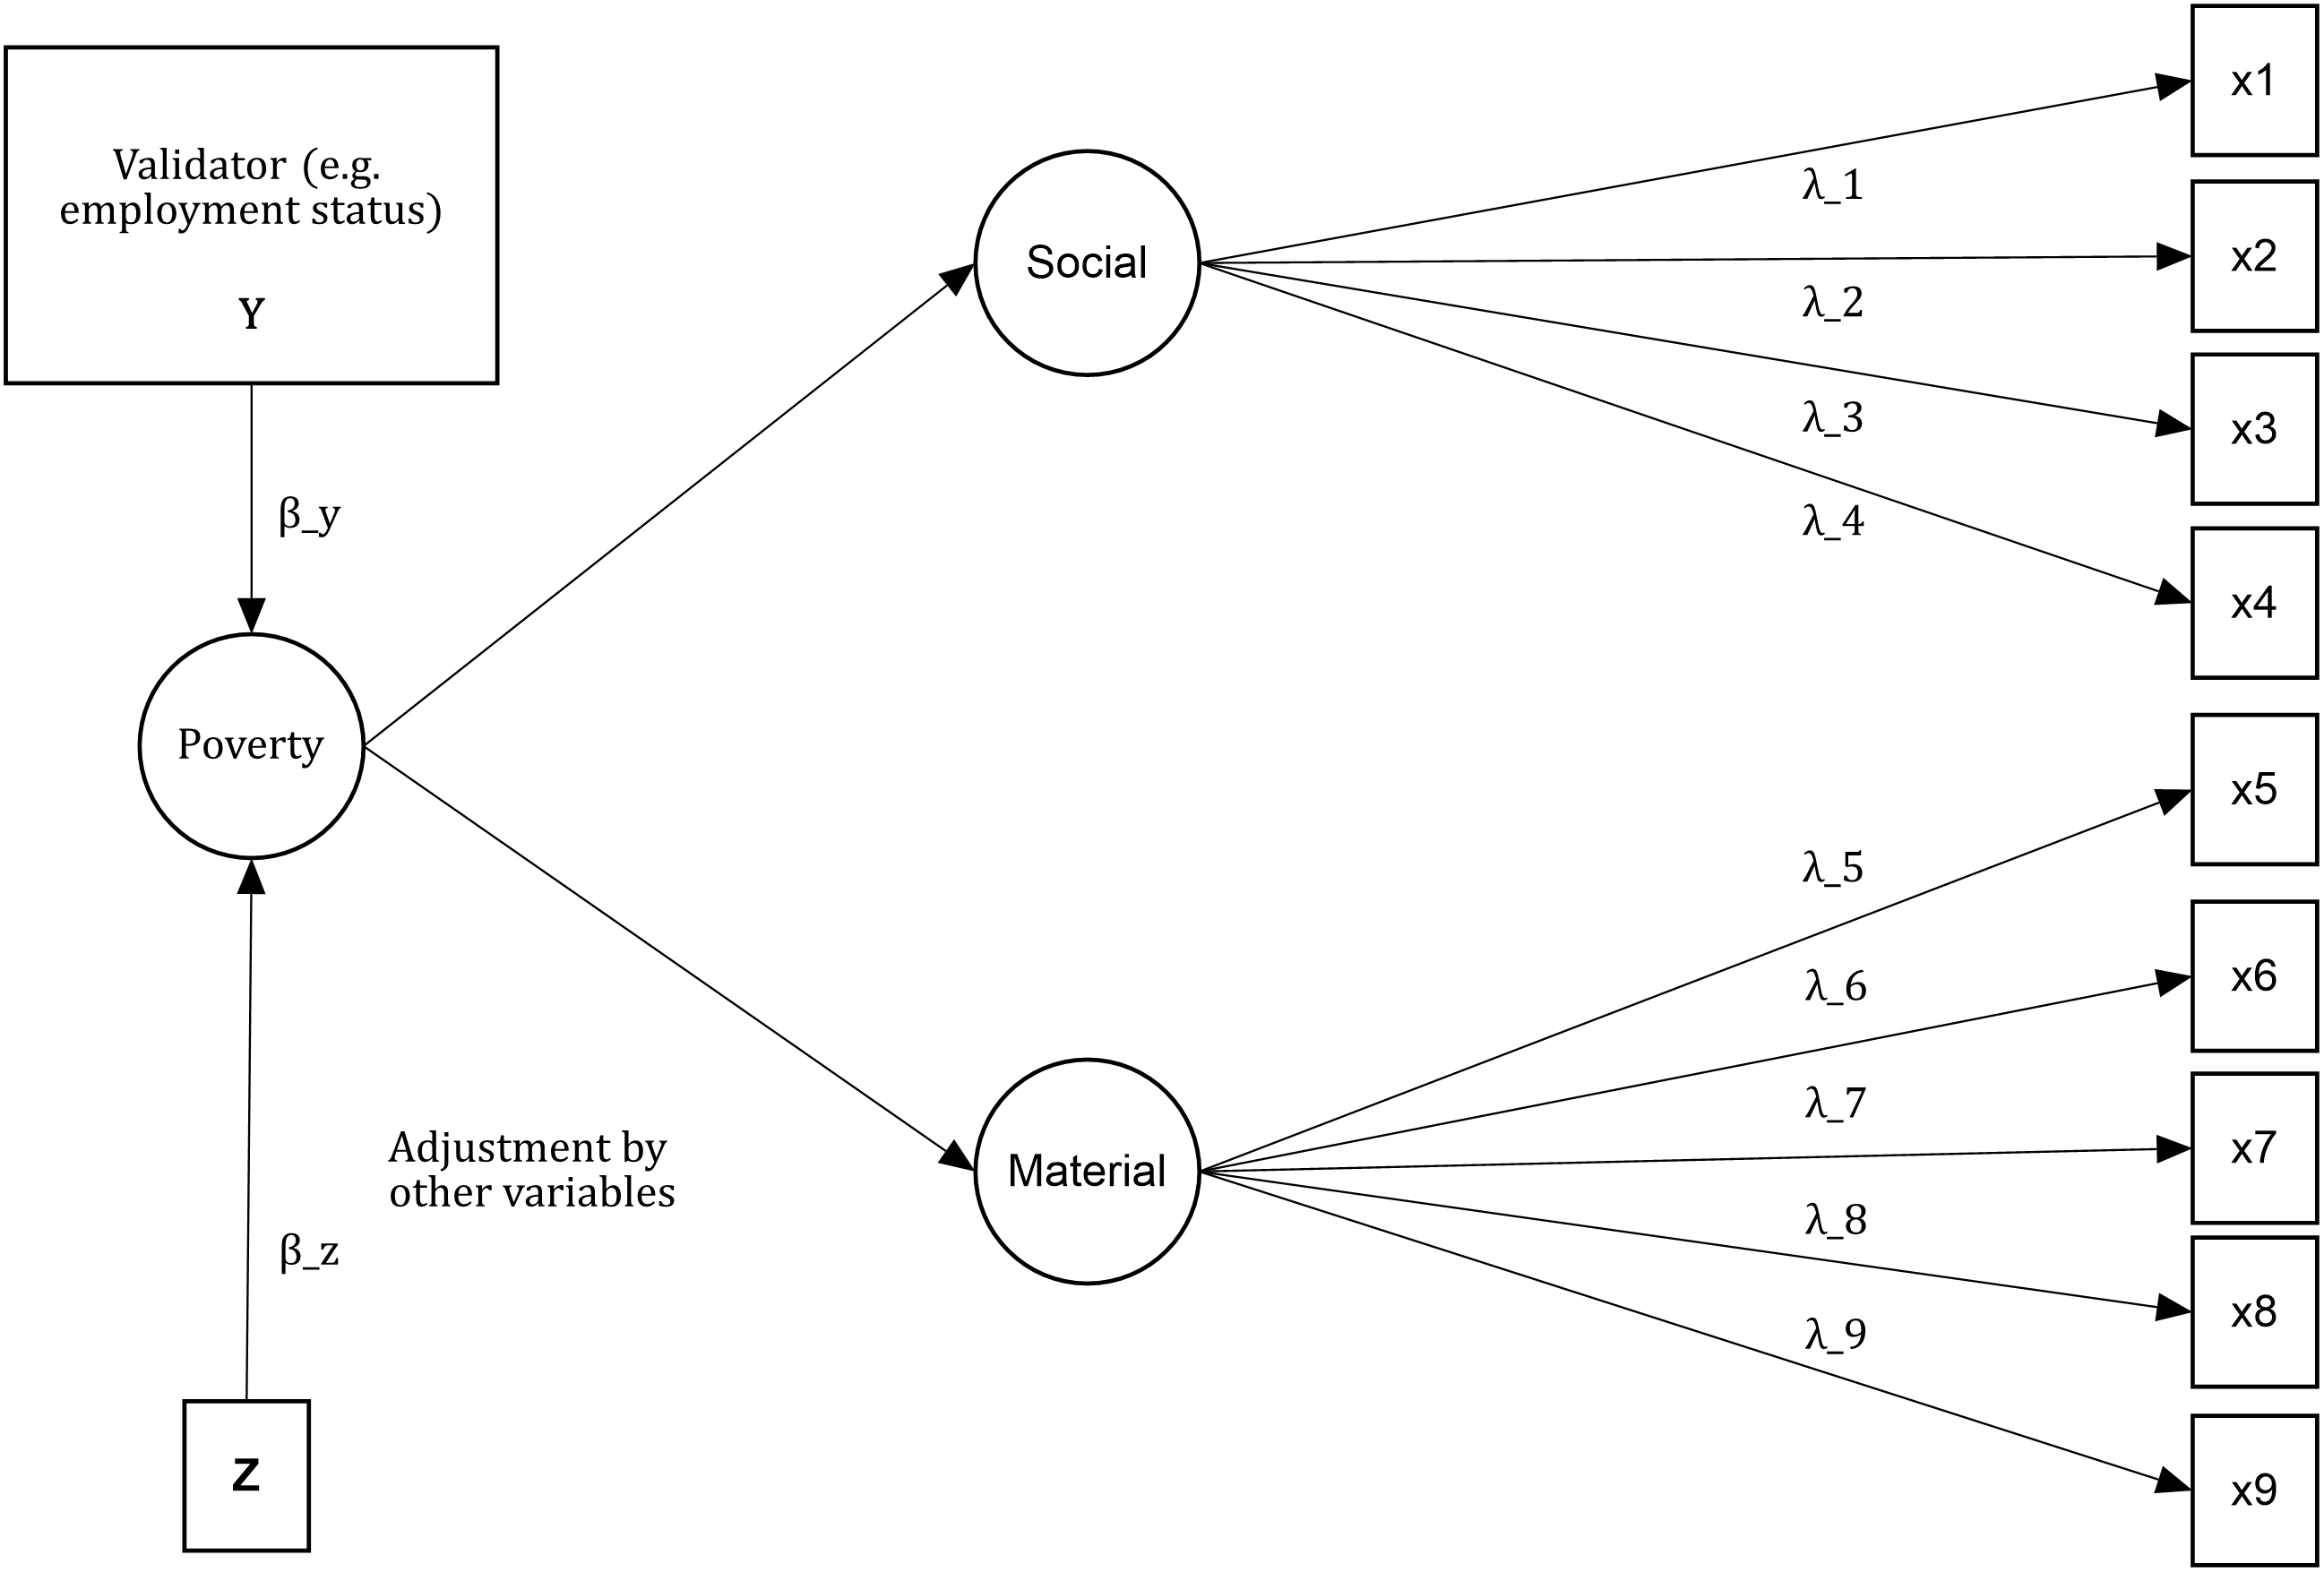
\includegraphics[width=\textwidth]{val_md_MIMIC} 

}

\caption{This is a visual representation of a MIMIC criterion validation of a reduced version of the theoretical model of Townsend}\label{fig:valmdmimic}
\end{figure}

\hypertarget{construct-validity}{%
\subsection{Construct validity}\label{construct-validity}}

Construct validity is an ongoing process and it is part of a unified framework of validity. Model specification is central in a statistical framework to measure poverty. This entails making explicit assumptions about the number, type and nature of the dimensions and its indicators. It also involves making assumptions about how the model should behave, i.e.~people with multiple deprivation should be more deprived than people with a single or no deprivations, for example. Construct validity comprises different sorts of evidence on the different hypothesis of the measurement model. To ilustrate this we will use the Multidimensional Poverty Measure of acute poverty.

\begin{itemize}
\tightlist
\item
  Multidimensional poverty has three substantive dimensions: education, health and standard of living.
\item
  These dimensions are clearly distinguishable (discriminant validity).
\item
  The indicators of each dimensions are adequate manifestations of deprivation of education, health and standard of living (classification of indicators).
\item
  The indicators of each dimensions equally account by for variation of the sub-dimensions (within-dimension weights).
\end{itemize}

The four hypothesis underpin the measurement model of poverty of the MPI. These are ordered from the more general to the most specific. How then these assumptions could be tested. Measurement theory has developed factor models for such a purpose. These models have evolved to such extent that the most powerful factor model could be used to test in one model a number of hypothesis. There are two main ways to conduct factor analysis: exploratory and confirmatory. This book puts emphasis on the second kind as it soughs to encourage the development of scales based on theory and not on what the available data says. The label ``Confirmatory'' is ambitious in that it suggest that we confirm that our model is right. This, of course, is never possible. The best we can do is to assess whether the model is not a bad one, which does not necessarily means that is the correct one.

Measurement models have a series of parameters (item loadings, dimension loadings, item thresholds and errors). Confirmatory factor analysis (CFA) is a way to estimate the value of the parameters in question and assess the extent to which the model reproduces the observable relationships among the indicators. This is no different from any experiment where given some assumptions, researchers compute if their model of reality is matched by observation. CFA models aim to assess if the presumed model of poverty seems to hold given the data, i.e.~whether there is any indication that there are three dimensions, the indicators seem to relate to these dimensions and the contribution of the indicators is equally important or not within dimensions.

To explain the theory of CFA models is necessary to bring back equations \eqref{eq:model1} and \eqref{eq:model2}.

\begin{equation}
 x_{ij} = \lambda_{ij} \eta_j + \varepsilon_ij   
\end{equation}

\begin{equation}
 \eta_j = \gamma_{j} \zeta  + \xi
\end{equation}

These equations represent a hierarchical Confirmatory Factor model. These make our measurement model testable using a method that was developed for such purpose. This model will tell us: if the three dimensions \(\eta_j\) (\(j=1,2,3\)) is an adequate representation of poverty. It will also tell us if the indicators are manifest (\(\lambda_{ij}\)) of the presumed dimensions, and whether the loadings are equal or not within dimensions.

How does CFA assesses whether a model matches observation? CFA estimates a series of parameters that produce a variance-covariance matrix (\(\Sigma\)) that approximates as closely as possible the observed variance-covariance matrix (\(S\)). Therefore, the goal in CFA is to find a set of parameters that best reproduces the input matrix. This process is achieved by minimizing the difference between \(\Sigma\) and \(S\). Maximum Likelihood (ML) is one of the preferred methods to estimate the minimizing function \(F_{ML}\) (see p.~72 and 73 for an explanation)(Brown, \protect\hyperlink{ref-Brown2006}{2006}). There are, nonetheless, several estimating procedures that are more or less adequate depending on the nature of the data. One of the most useful and adequate for the kind of data in poverty measurement (categorical data with large samples) is robust weighted least squares (WLSMV) as it is faster than ML and is asymptotic distribution free. \(F_{ML}\) is very useful because it provides standard errors (SEs) of the estimates but also because it can be used for the calculation of several indices of goodness-of-fit which tell how poor or good the model is.

\(F_{ML}\) is used for several goodness-of-fit indices. An absolute index is \(\chi^2\) which operates with the null hypothesis that \(S=\Sigma\). When rejected, it tell that the proposed model is not good enough to reproduce \(S\). In other words, the number, type of dimensions and indicators do not result in an adequate representation of the construct. \(\chi^2 = F_{ML}(N-1)\) and thus is sensible to sample size and based on a very stringent hypothesis that \(S=\Sigma\).

A relative index of goodness-of-fit is root mean square error of approximation (RMSEA) (Steiger, \protect\hyperlink{ref-Steiger1980}{1980}). This index looks at the extent to which a model is a reasonable approximation in the population. This index is sensible to the number of parameters in the model but insensitive to sample size.

Comparative fit indices use a baseline model (typically a null model) as reference to evaluate the fit of the proposed model. These indexes often look more favourable than the strict \(\chi^2\). Extensive Monte Carlo studies have found that these indexes are nonetheless trustworthy and well-behaved. The Comparative Fit Index (CFI) is one of the most widely used. It varies between 0 and 1 where values closer to 1 indicate a good model fit. The Tucker-Lewis index (TLI) is another popular alternative which includes a penalty function for adding more parameters that do not necessarily improve the fit of the model. It typically has values between 0 and 1, where again closer to 1 implies a relatively good model fit.

Several Monte Carlo studies have been conducted to assess the behaviour of these indices (Bentler, \protect\hyperlink{ref-Bentler2007}{2007}; Browne, Cudeck, \& others, \protect\hyperlink{ref-Browne1993}{1993}; Hu \& Bentler, \protect\hyperlink{ref-Hu1999}{1999}; Rigdon, \protect\hyperlink{ref-Rigdon1996}{1996}). From these studies it has been possible to have an approximation to the values of the indices that often indicate a good fit. These values are summarised as follows:

\begin{longtable}[]{@{}lcc@{}}
\caption{\label{tab:cfafitstats} Summary of the suggested cut off for the goodness-of-fit statistics.
The values of RMSEA, CFI and TLI need to be taken as an approximation.}\tabularnewline
\toprule
Index & Range values & Poor model fit rule\tabularnewline
\midrule
\endfirsthead
\toprule
Index & Range values & Poor model fit rule\tabularnewline
\midrule
\endhead
\(\chi^2\) & p-values 1-0 & \(p<.05\)\tabularnewline
\(RMSEA\) & p-values 1-0 & \(p>.06\)\tabularnewline
\(CFI\) & \(1-0\) & \(<.95\)\tabularnewline
\(TLI\) & \(1-0\) & \(<.95\)\tabularnewline
\bottomrule
\end{longtable}

Factor loadings are often thought as a measure of item-reliability (see Section @ref()). So how does the factor loading values fit in a validity analysis? There is no consensus about threating factor loadings as measures of item validity. Only and only if the measure is proven to be valid in some way, it is possible to frame item loadings in terms of validity. In such a context, the square of the factor loadings equals the amount of variance in the indicator explained by the common factor (i.e.~communality). Because the factor loadings capture the relationship of each indicator with the latent variable, they can be seen as the optimal weights of the model given the data. Therefore, a test of equality of loadings within dimensional can be used to assess whether using such kind of weighting is reasonable or not. The next section shows how these tests work but the idea is to assess the extent to which \(\lambda_{11}=\lambda_{21}=\lambda_{31}\), for example for three items in dimension \(j=1\).

\hypertarget{validity-assessment}{%
\section{Validity assessment}\label{validity-assessment}}

\hypertarget{criterion-validity-1}{%
\subsection{Criterion Validity}\label{criterion-validity-1}}

Criterion or predictive validity holds when there is a correlation between an scale and an alternative measure on the cause or effects of the construct of interest. In poverty research, this kind of validation has been used in the empirical literature (Gordon, \protect\hyperlink{ref-Gordon2010}{2010}; Guio et al., \protect\hyperlink{ref-Guio2012}{2012}; Nandy \& Pomati, \protect\hyperlink{ref-Nandy2015}{2015}). We will again use our simulated multidimensional measure to illustrate how a validation exercise can be undertaken and to underline some issue researchers might find in practice.

Fitting a regression model to assess the relationship between a proposed index and an alternative measure is a common approach to assess predictive validity. To illustrate how this kind of validation works, we will use the simulated data (``Rel\_MD\_data\_1\_1.dat''). This data set contains the nine manifest variables (x1-x9) plus the two unreliable indicators(x10-x11). Three variables were simulated as alternative measures. One is a ``perfect'' measure of the resources available for each household in the sample. So in principle, this measure ranks the households according to their potential to fulfil their needs. The measure is expressed in monetary terms to facilitate the interpretation. Education years of the household head and occupation (skill scale) are two predictors of the living standards of the households. These two variables reflect the often common case where the survey was not designed with a validator in mind. We will use the variable ``hh\_members'' to adjust the estimates.

\begin{Shaded}
\begin{Highlighting}[]
\KeywordTok{library}\NormalTok{(plyr)}
\NormalTok{Rel_MD_}\DecValTok{1}\NormalTok{<-}\KeywordTok{read.table}\NormalTok{(}\StringTok{"Rel_MD_data_1_1.dat"}\NormalTok{)}
\NormalTok{Rel_MD_}\DecValTok{1}\OperatorTok{$}\NormalTok{ds<-}\KeywordTok{rowSums}\NormalTok{(Rel_MD_}\DecValTok{1}\NormalTok{[,}\KeywordTok{c}\NormalTok{(}\DecValTok{1}\OperatorTok{:}\DecValTok{9}\NormalTok{)])}
\KeywordTok{colnames}\NormalTok{(Rel_MD_}\DecValTok{1}\NormalTok{)<-}\KeywordTok{c}\NormalTok{(}\StringTok{"x1"}\NormalTok{,}\StringTok{"x2"}\NormalTok{,}\StringTok{"x3"}\NormalTok{,}\StringTok{"x4"}\NormalTok{,}\StringTok{"x5"}\NormalTok{,}\StringTok{"x6"}\NormalTok{,}
                      \StringTok{"x7"}\NormalTok{,}\StringTok{"x8"}\NormalTok{,}\StringTok{"x9"}\NormalTok{,}\StringTok{"x10"}\NormalTok{,}\StringTok{"x11"}\NormalTok{,}
                      \StringTok{"resources"}\NormalTok{,}\StringTok{"educ_yr"}\NormalTok{,}\StringTok{"occupation"}\NormalTok{,}
                      \StringTok{"hh_members"}\NormalTok{,}\StringTok{"class"}\NormalTok{,}\StringTok{"ds"}\NormalTok{)}
\NormalTok{Rel_MD_}\DecValTok{1}\NormalTok{[}\DecValTok{1}\OperatorTok{:}\DecValTok{5}\NormalTok{,}\DecValTok{1}\OperatorTok{:}\DecValTok{11}\NormalTok{]}
\end{Highlighting}
\end{Shaded}

\begin{verbatim}
##   x1 x2 x3 x4 x5 x6 x7 x8 x9 x10 x11
## 1  1  1  1  1  0  0  0  0  0   0   0
## 2  0  0  0  0  0  0  0  0  0   0   0
## 3  0  0  0  1  0  0  0  0  0   0   0
## 4  1  1  0  0  0  0  1  0  0   0   0
## 5  1  0  0  0  0  0  0  0  0   1   1
\end{verbatim}

\begin{Shaded}
\begin{Highlighting}[]
\NormalTok{Rel_MD_}\DecValTok{1}\NormalTok{[}\DecValTok{1}\OperatorTok{:}\DecValTok{5}\NormalTok{,}\DecValTok{12}\OperatorTok{:}\DecValTok{15}\NormalTok{]}
\end{Highlighting}
\end{Shaded}

\begin{verbatim}
##   resources educ_yr occupation hh_members
## 1  3276.687       6          4          5
## 2  7508.982      15          2          1
## 3  7183.707       8          5          2
## 4  1574.356       6          2          7
## 5  2210.297       9          5          4
\end{verbatim}

One way to conduct the validation analysis consists in estimating the association between the manifest variables of our index with the validator. This can be simply done by fitting a series of regression models. Because deprivations are binary variables, we need to use a Generalised Linear Model (GLM) with the appropriate distribution. Relative Risk Ratios (RRR) are easier to interpret, so we will fit a Poisson model with log link to obtain the RRRs. Of course, there is no problem in estimating odd-ratios as here we are interested in looking at the association between variables.

In total we have 11 dependent variables (x1-x11) and, thus 11 models. In principle, x1-x11 resulted unreliable and should have been dropped from the analysis but we will keep them just to discuss some connections between reliability and validity. We will create a simple function \texttt{lms()} below to loop across the deprivation indicators. We will also transform the resources to get a more sensible metric.

\begin{Shaded}
\begin{Highlighting}[]
\NormalTok{Rel_MD_}\DecValTok{1}\OperatorTok{$}\NormalTok{resources<-Rel_MD_}\DecValTok{1}\OperatorTok{$}\NormalTok{resources}\OperatorTok{*}\NormalTok{.}\DecValTok{01}

\NormalTok{lms<-}\ControlFlowTok{function}\NormalTok{(index)}
\NormalTok{\{}
\NormalTok{  fit<-}\KeywordTok{glm}\NormalTok{(Rel_MD_}\DecValTok{1}\NormalTok{[,index] }\OperatorTok{~}\StringTok{ }\NormalTok{Rel_MD_}\DecValTok{1}\OperatorTok{$}\NormalTok{resources }\OperatorTok{+}
\StringTok{                              }\NormalTok{Rel_MD_}\DecValTok{1}\OperatorTok{$}\NormalTok{hh_members,}
           \DataTypeTok{family=}\KeywordTok{poisson}\NormalTok{(}\DataTypeTok{link=}\StringTok{"log"}\NormalTok{))}
  \KeywordTok{exp}\NormalTok{(}\KeywordTok{cbind}\NormalTok{(}\DataTypeTok{OR =} \KeywordTok{coef}\NormalTok{(fit), }\KeywordTok{confint}\NormalTok{(fit)))}
\NormalTok{\}}

\NormalTok{coefs<-}\KeywordTok{lapply}\NormalTok{(}\DecValTok{1}\OperatorTok{:}\DecValTok{11}\NormalTok{,lms)}

\NormalTok{coefs[[}\DecValTok{1}\NormalTok{]]}
\end{Highlighting}
\end{Shaded}

We could check each of the outputs in list \texttt{coefs} but it is easier to plot the RRRs of resources for each one of the 11 variables. We will not show the code here but one could just simply extract the coefficients and use \texttt{ggplot2()} to produce the graph. The coefficients are displayed with 95\% confidence intervals in plot\textasciitilde{}\ref{fig:val1}\footnote{Here we are using classic or frequentist statistics. There are many problems around the use of p-values. We will be careful in the interpretation as the kind of test we run here is very conservative, i.e. the association is zero. We are not assessing whether is positive or negative. But we should do it in future editions.}. The null hypothesis in this model is that there is no relationship between resources and deprivation. For items x1-x9 we see that the difference seems to be different from zero and that the estimates are likely to be less than one. This suggests the higher the resources and lower the chances of being deprived. This is in line with our expectation. For items x10 and x11, however, we found no relationship at all. This is an indication that both items are unreliable and invalid. This reinforces our previous suspicion that these two items are not useful to measure poverty.

\begin{Shaded}
\begin{Highlighting}[]
\NormalTok{coefs<-}\KeywordTok{lapply}\NormalTok{(coefs, }\ControlFlowTok{function}\NormalTok{(x) }\KeywordTok{unlist}\NormalTok{(x[}\DecValTok{2}\NormalTok{,]))}
\NormalTok{coefs<-}\StringTok{ }\KeywordTok{as.matrix}\NormalTok{(}\KeywordTok{matrix}\NormalTok{(}\KeywordTok{unlist}\NormalTok{(coefs), }\DataTypeTok{nrow=}\KeywordTok{length}\NormalTok{(coefs), }\DataTypeTok{byrow=}\NormalTok{T))}
\NormalTok{coefs<-}\KeywordTok{data.frame}\NormalTok{(}\KeywordTok{rbind}\NormalTok{(coefs[,}\KeywordTok{c}\NormalTok{(}\DecValTok{1}\NormalTok{,}\DecValTok{2}\NormalTok{,}\DecValTok{3}\NormalTok{)]))}

\NormalTok{coefs}\OperatorTok{$}\NormalTok{item <-}\StringTok{ }\KeywordTok{rep}\NormalTok{(}\KeywordTok{c}\NormalTok{(}\StringTok{"x1"}\NormalTok{,}\StringTok{"x2"}\NormalTok{,}\StringTok{"x3"}\NormalTok{,}\StringTok{"x4"}\NormalTok{,}\StringTok{"x5"}\NormalTok{,}\StringTok{"x6"}\NormalTok{,}
                      \StringTok{"x7"}\NormalTok{,}\StringTok{"x8"}\NormalTok{,}\StringTok{"x9"}\NormalTok{,}\StringTok{"x10"}\NormalTok{,}\StringTok{"x11"}\NormalTok{),}\DecValTok{1}\NormalTok{)}
\NormalTok{coefs}\OperatorTok{$}\NormalTok{var<-}\KeywordTok{c}\NormalTok{(}\KeywordTok{rep}\NormalTok{(}\StringTok{"Resources (*100)"}\NormalTok{, }\DecValTok{11}\NormalTok{))}
\NormalTok{coefs}
\end{Highlighting}
\end{Shaded}

We can simply plot the coefficients of each variable using the object \texttt{coefs} and \texttt{ggplot2()} as follows:

\begin{Shaded}
\begin{Highlighting}[]
\NormalTok{p<-}\StringTok{ }\KeywordTok{ggplot}\NormalTok{(coefs, }\KeywordTok{aes}\NormalTok{(}\DataTypeTok{x=}\NormalTok{item,}\DataTypeTok{y=}\NormalTok{X1)) }\OperatorTok{+}\StringTok{ }\KeywordTok{geom_point}\NormalTok{() }\OperatorTok{+}\StringTok{  }
\StringTok{  }\KeywordTok{geom_errorbar}\NormalTok{(}\KeywordTok{aes}\NormalTok{(}\DataTypeTok{ymin=}\NormalTok{X2, }\DataTypeTok{ymax=}\NormalTok{X3)) }\OperatorTok{+}
\StringTok{ }\KeywordTok{theme_bw}\NormalTok{() }\OperatorTok{+}\StringTok{ }\KeywordTok{scale_y_continuous}\NormalTok{(}\DataTypeTok{trans =} \StringTok{'log10'}\NormalTok{, }\DataTypeTok{limits =} \KeywordTok{c}\NormalTok{(.}\DecValTok{9}\NormalTok{, }\FloatTok{1.1}\NormalTok{))}
\NormalTok{p }\OperatorTok{+}\StringTok{ }\KeywordTok{facet_grid}\NormalTok{(. }\OperatorTok{~}\StringTok{ }\NormalTok{var) }\OperatorTok{+}\StringTok{ }\KeywordTok{labs}\NormalTok{(}\DataTypeTok{y=}\StringTok{"Relative Risk Ratios"}\NormalTok{) }\OperatorTok{+}\StringTok{ }\KeywordTok{geom_hline}\NormalTok{(}\DataTypeTok{yintercept=}\DecValTok{1}\NormalTok{, }\DataTypeTok{linetype=}\StringTok{"dashed"}\NormalTok{,}
                \DataTypeTok{color =} \StringTok{"red"}\NormalTok{, }\DataTypeTok{size=}\DecValTok{2}\NormalTok{)}
\end{Highlighting}
\end{Shaded}

\begin{figure}
\centering
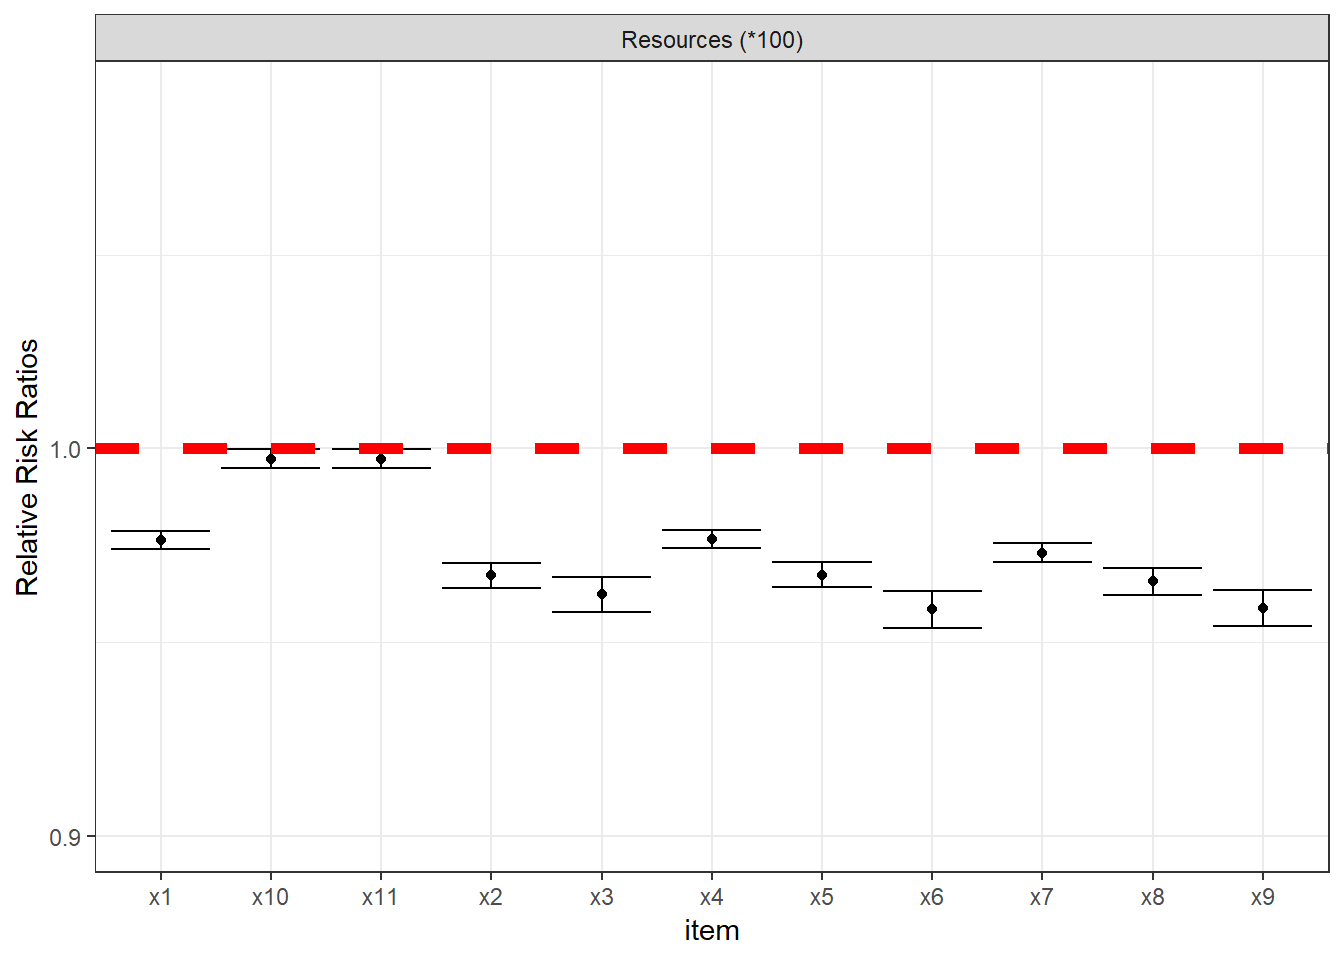
\includegraphics{PM_Book_files/figure-latex/val1-1.png}
\caption{\label{fig:val1}This plot shows the Relative Risk Ratios for the resources variable, adjusted by the household size. Having more resources reduces the risk of being deprived of the item x, as expected.}
\end{figure}

Now we will go through the case of the lack of a validator. Most of the time researchers will lack a validator that was designed a priori. In these circumstances researchers need to use variables that predict poverty. Education attainment of the household head and occupation status are one of the two best predictors of poverty. We will rewrite our \texttt{lms()} function to fit a series of models using both education and occupation. All models adjusted by the household size. Again we will fit a GLM to obtain relative risks.

\begin{Shaded}
\begin{Highlighting}[]
\NormalTok{lms<-}\ControlFlowTok{function}\NormalTok{(index)}
\NormalTok{\{}
\NormalTok{  fit<-}\KeywordTok{glm}\NormalTok{(Rel_MD_}\DecValTok{1}\NormalTok{[,index] }\OperatorTok{~}\StringTok{ }\NormalTok{Rel_MD_}\DecValTok{1}\OperatorTok{$}\NormalTok{occupation }\OperatorTok{+}
\StringTok{                              }\NormalTok{Rel_MD_}\DecValTok{1}\OperatorTok{$}\NormalTok{educ_yr }\OperatorTok{+}
\StringTok{                              }\NormalTok{Rel_MD_}\DecValTok{1}\OperatorTok{$}\NormalTok{hh_members,}
           \DataTypeTok{family=}\KeywordTok{poisson}\NormalTok{(}\DataTypeTok{link=}\StringTok{"log"}\NormalTok{))}
  \KeywordTok{exp}\NormalTok{(}\KeywordTok{cbind}\NormalTok{(}\DataTypeTok{OR =} \KeywordTok{coef}\NormalTok{(fit), }\KeywordTok{confint}\NormalTok{(fit)))}
\NormalTok{\}}

\NormalTok{coefs<-}\KeywordTok{lapply}\NormalTok{(}\DecValTok{1}\OperatorTok{:}\DecValTok{11}\NormalTok{,lms)}
\end{Highlighting}
\end{Shaded}

\begin{verbatim}
## Waiting for profiling to be done...
## Waiting for profiling to be done...
## Waiting for profiling to be done...
## Waiting for profiling to be done...
## Waiting for profiling to be done...
## Waiting for profiling to be done...
## Waiting for profiling to be done...
## Waiting for profiling to be done...
## Waiting for profiling to be done...
## Waiting for profiling to be done...
## Waiting for profiling to be done...
\end{verbatim}

\begin{Shaded}
\begin{Highlighting}[]
\NormalTok{coefs[[}\DecValTok{1}\NormalTok{]]}
\end{Highlighting}
\end{Shaded}

\begin{verbatim}
##                            OR     2.5 %    97.5 %
## (Intercept)         0.6866791 0.5503763 0.8554189
## Rel_MD_1$occupation 1.0531859 1.0377362 1.0688189
## Rel_MD_1$educ_yr    0.9206710 0.9051449 0.9364577
## Rel_MD_1$hh_members 1.0163837 0.9939741 1.0391996
\end{verbatim}

\begin{Shaded}
\begin{Highlighting}[]
\NormalTok{coefs<-}\KeywordTok{lapply}\NormalTok{(coefs, }\ControlFlowTok{function}\NormalTok{(x) }\KeywordTok{unlist}\NormalTok{(x[}\DecValTok{2}\OperatorTok{:}\DecValTok{3}\NormalTok{,]))}
\NormalTok{coefs<-}\StringTok{ }\KeywordTok{as.matrix}\NormalTok{(}\KeywordTok{matrix}\NormalTok{(}\KeywordTok{unlist}\NormalTok{(coefs), }\DataTypeTok{nrow=}\KeywordTok{length}\NormalTok{(coefs), }\DataTypeTok{byrow=}\NormalTok{T))}
\NormalTok{coefs<-}\KeywordTok{data.frame}\NormalTok{(}\KeywordTok{rbind}\NormalTok{(coefs[,}\KeywordTok{c}\NormalTok{(}\DecValTok{1}\NormalTok{,}\DecValTok{3}\NormalTok{,}\DecValTok{5}\NormalTok{)],coefs[,}\KeywordTok{c}\NormalTok{(}\DecValTok{2}\NormalTok{,}\DecValTok{4}\NormalTok{,}\DecValTok{6}\NormalTok{)]))}

\NormalTok{coefs}\OperatorTok{$}\NormalTok{item <-}\StringTok{ }\KeywordTok{rep}\NormalTok{(}\KeywordTok{c}\NormalTok{(}\StringTok{"x1"}\NormalTok{,}\StringTok{"x2"}\NormalTok{,}\StringTok{"x3"}\NormalTok{,}\StringTok{"x4"}\NormalTok{,}\StringTok{"x5"}\NormalTok{,}\StringTok{"x6"}\NormalTok{,}
                      \StringTok{"x7"}\NormalTok{,}\StringTok{"x8"}\NormalTok{,}\StringTok{"x9"}\NormalTok{,}\StringTok{"x10"}\NormalTok{,}\StringTok{"x11"}\NormalTok{),}\DecValTok{2}\NormalTok{)}
\NormalTok{coefs}\OperatorTok{$}\NormalTok{var<-}\KeywordTok{c}\NormalTok{(}\KeywordTok{rep}\NormalTok{(}\StringTok{"Occupation (Skill) scale"}\NormalTok{, }\DecValTok{11}\NormalTok{), }\KeywordTok{rep}\NormalTok{(}\StringTok{"Education years"}\NormalTok{, }\DecValTok{11}\NormalTok{))}
\NormalTok{coefs}
\end{Highlighting}
\end{Shaded}

\begin{verbatim}
##           X1        X2        X3 item                      var
## 1  1.0531859 1.0377362 1.0688189   x1 Occupation (Skill) scale
## 2  1.0691741 1.0489816 1.0896804   x2 Occupation (Skill) scale
## 3  1.0781765 1.0510322 1.1058950   x3 Occupation (Skill) scale
## 4  1.0590273 1.0433546 1.0748872   x4 Occupation (Skill) scale
## 5  1.0721107 1.0517452 1.0927967   x5 Occupation (Skill) scale
## 6  1.0993761 1.0713526 1.1280058   x6 Occupation (Skill) scale
## 7  1.0610757 1.0448192 1.0775352   x7 Occupation (Skill) scale
## 8  1.0728834 1.0512460 1.0948827   x8 Occupation (Skill) scale
## 9  1.1084601 1.0802115 1.1373136   x9 Occupation (Skill) scale
## 10 1.0001156 0.9817638 1.0187286  x10 Occupation (Skill) scale
## 11 1.0087886 0.9905182 1.0273171  x11 Occupation (Skill) scale
## 12 0.9206710 0.9051449 0.9364577   x1          Education years
## 13 0.8977545 0.8780443 0.9178932   x2          Education years
## 14 0.8758993 0.8500184 0.9025356   x3          Education years
## 15 0.9311522 0.9153057 0.9472680   x4          Education years
## 16 0.9052537 0.8851807 0.9257679   x5          Education years
## 17 0.8979686 0.8708921 0.9258545   x6          Education years
## 18 0.9150086 0.8987985 0.9315038   x7          Education years
## 19 0.9029371 0.8816859 0.9246844   x8          Education years
## 20 0.8974289 0.8704803 0.9251801   x9          Education years
## 21 0.9848866 0.9650072 1.0051781  x10          Education years
## 22 0.9958716 0.9759022 1.0162522  x11          Education years
\end{verbatim}

Once the models have been fitted, we could proceed to inspect the parameters. To inspect them we produce two plots shown in figure\textasciitilde\ref{fig:val2}. The plot show the RRRs for both education and occupation adjusted by the household size. There is no evidence to support an association between items x10 and x11 and both predictors of poverty. In contrast, education and occupation predict an decrease and increase in the likelihood of being deprived of items x1-x9. On this basis we could conclude that our scale has criterion validity.

\begin{Shaded}
\begin{Highlighting}[]
\NormalTok{p<-}\StringTok{ }\KeywordTok{ggplot}\NormalTok{(coefs, }\KeywordTok{aes}\NormalTok{(}\DataTypeTok{x=}\NormalTok{item,}\DataTypeTok{y=}\NormalTok{X1)) }\OperatorTok{+}\StringTok{ }\KeywordTok{geom_point}\NormalTok{() }\OperatorTok{+}\StringTok{  }
\StringTok{  }\KeywordTok{geom_errorbar}\NormalTok{(}\KeywordTok{aes}\NormalTok{(}\DataTypeTok{ymin=}\NormalTok{X2, }\DataTypeTok{ymax=}\NormalTok{X3)) }\OperatorTok{+}
\StringTok{ }\KeywordTok{theme_bw}\NormalTok{() }\OperatorTok{+}\StringTok{ }\KeywordTok{scale_y_continuous}\NormalTok{(}\DataTypeTok{trans =} \StringTok{'log10'}\NormalTok{, }\DataTypeTok{limits =} \KeywordTok{c}\NormalTok{(.}\DecValTok{8}\NormalTok{, }\FloatTok{1.2}\NormalTok{))}
\NormalTok{p }\OperatorTok{+}\StringTok{ }\KeywordTok{facet_grid}\NormalTok{(. }\OperatorTok{~}\StringTok{ }\NormalTok{var) }\OperatorTok{+}\StringTok{ }\KeywordTok{labs}\NormalTok{(}\DataTypeTok{y=}\StringTok{"Relative Risk Ratios"}\NormalTok{) }\OperatorTok{+}\StringTok{ }\KeywordTok{geom_hline}\NormalTok{(}\DataTypeTok{yintercept=}\DecValTok{1}\NormalTok{, }\DataTypeTok{linetype=}\StringTok{"dashed"}\NormalTok{,}
                \DataTypeTok{color =} \StringTok{"red"}\NormalTok{, }\DataTypeTok{size=}\DecValTok{2}\NormalTok{)}
\end{Highlighting}
\end{Shaded}

\begin{figure}
\centering
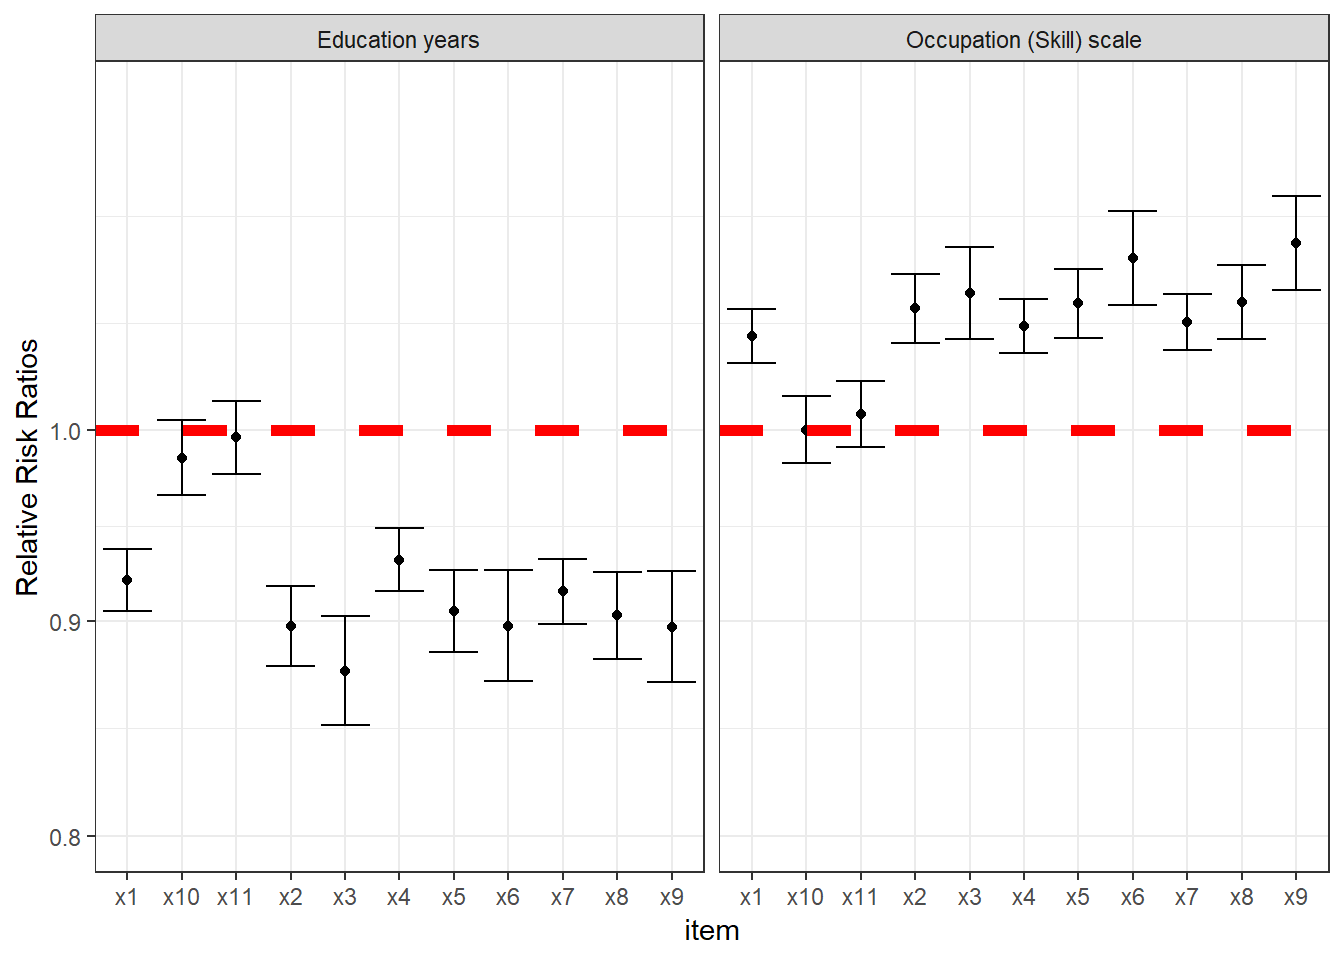
\includegraphics{PM_Book_files/figure-latex/val2-1.png}
\caption{\label{fig:val2}This plot shows the Relative Risk Ratios for each item using two validators (adjusted by the total household members)}
\end{figure}

\begin{Shaded}
\begin{Highlighting}[]
\NormalTok{p<-}\StringTok{ }\KeywordTok{ggplot}\NormalTok{(coefs, }\KeywordTok{aes}\NormalTok{(}\DataTypeTok{x=}\NormalTok{item,}\DataTypeTok{y=}\NormalTok{X1)) }\OperatorTok{+}\StringTok{ }\KeywordTok{geom_point}\NormalTok{() }\OperatorTok{+}\StringTok{  }
\StringTok{  }\KeywordTok{geom_errorbar}\NormalTok{(}\KeywordTok{aes}\NormalTok{(}\DataTypeTok{ymin=}\NormalTok{X2, }\DataTypeTok{ymax=}\NormalTok{X3)) }\OperatorTok{+}
\StringTok{ }\KeywordTok{theme_bw}\NormalTok{() }\OperatorTok{+}\StringTok{ }\KeywordTok{scale_y_continuous}\NormalTok{(}\DataTypeTok{trans =} \StringTok{'log10'}\NormalTok{, }\DataTypeTok{limits =} \KeywordTok{c}\NormalTok{(.}\DecValTok{8}\NormalTok{, }\FloatTok{1.2}\NormalTok{))}

\KeywordTok{jpeg}\NormalTok{(}\StringTok{"val_rrrs.jpg"}\NormalTok{, }\DataTypeTok{units=}\StringTok{"cm"}\NormalTok{, }\DataTypeTok{width=}\DecValTok{10}\NormalTok{, }\DataTypeTok{height=}\DecValTok{10}\NormalTok{, }\DataTypeTok{res=}\DecValTok{300}\NormalTok{)}
\NormalTok{p }\OperatorTok{+}\StringTok{ }\KeywordTok{facet_grid}\NormalTok{(. }\OperatorTok{~}\StringTok{ }\NormalTok{var) }\OperatorTok{+}\StringTok{ }\KeywordTok{labs}\NormalTok{(}\DataTypeTok{y=}\StringTok{"Relative Risk Ratios"}\NormalTok{) }\OperatorTok{+}\StringTok{ }\KeywordTok{geom_hline}\NormalTok{(}\DataTypeTok{yintercept=}\DecValTok{1}\NormalTok{, }\DataTypeTok{linetype=}\StringTok{"dashed"}\NormalTok{,}
                \DataTypeTok{color =} \StringTok{"red"}\NormalTok{, }\DataTypeTok{size=}\DecValTok{2}\NormalTok{)}
\KeywordTok{dev.off}\NormalTok{()}
\end{Highlighting}
\end{Shaded}

\hypertarget{construct-validity-1}{%
\subsection{Construct Validity}\label{construct-validity-1}}

Validity now is seen under a unified approach that looks at different aspects of the extent to which our scale can be interpreted as it is supposed to- a measure of poverty. Predictive validity might be a useful way to check the predictive validity at item-level. However, such kind of validation tells nothing about the structure of the measure. In section @ref\{\} we mention that modern poverty research should walk toward the specification of measurement models so that researchers make their assumptions better. We have mention that our scale is a higher-order scale with three dimensions, each one measured by three items. Construct validity concerns with the assessment of the structure of our scale. We will address several hypothesis about our scale:

\begin{itemize}
\tightlist
\item
  Are three dimensions a sensible way to arrange our indicators?
\item
  Is a higher order factor present in our scale?
\item
  Is the contribution to the explanation of the variance of each item equal or unequal?
\end{itemize}

We will focus on the first two question for now. To assess the validity of our measure we will use CFA to assess whether our measurement model is an adequate representation of poverty given these data. A CFA explicitly asks the question about the capacity of a model to reproduce the observed data. The first step, thus, consists in specifying our model. We have done already this in section @ref\{\} when we estimated the reliability statistics \(\omega\) and \(\omega_h\). We will fit again the model using the \texttt{lavaan} R-package and Mplus. We will start with \texttt{lavaan} by specifying the \(MD_model\). As can be appreciated we are assuming three factors (f1 to f3) and a higher order factor h. We are also stating that the indicators are manifest of one factor, i.e.~we do not see x1 in f2 or f3. Then we can simply use the \texttt{sem()} function and tell that our items are categorical. We will store the output in the fit object.

\begin{Shaded}
\begin{Highlighting}[]
\NormalTok{MD_model <-}\StringTok{ ' f1  =~ x1 + x2 + x3}
\StringTok{              f2 =~ x4 + x5 + x6}
\StringTok{              f3   =~ x7 + x8 + x9}
\StringTok{               h =~ f1 + f2 + f3}
\StringTok{'}

\NormalTok{fit <-}\StringTok{ }\KeywordTok{sem}\NormalTok{(MD_model,}
           \DataTypeTok{data =}\NormalTok{ Rel_MD_}\DecValTok{1}\NormalTok{,}\DataTypeTok{ordered=}\KeywordTok{c}\NormalTok{(}\StringTok{"x1"}\NormalTok{,}\StringTok{"x2"}\NormalTok{,}\StringTok{"x3"}\NormalTok{,}\StringTok{"x4"}\NormalTok{,}\StringTok{"x5"}\NormalTok{,}
                                     \StringTok{"x6"}\NormalTok{,}\StringTok{"x7"}\NormalTok{,}\StringTok{"x8"}\NormalTok{,}\StringTok{"x9"}\NormalTok{))}
\end{Highlighting}
\end{Shaded}

Once the model has been estimated, we can request the global statistics of fit of our model saved in the fit object. To extract the statistics we will use the function \texttt{fitmeasures()}. We will request the \(\chi^2\) test (absolute fit), the CFI and TLI values and RMSEA (relative fit). The p-value of the \(\chi^2\) test suggest that we reject the hypothesis that the model does not reproduces the observed data. That means that dimensions, classification of the indicators and the presence of the higher order factor do a good job in representing the structure of the data. CFI, TLI and RMSEA point in the same direction.

\begin{Shaded}
\begin{Highlighting}[]
\NormalTok{chisq<-}\KeywordTok{fitmeasures}\NormalTok{(fit,}\DataTypeTok{fit.measures =} \KeywordTok{c}\NormalTok{(}\StringTok{"chisq"}\NormalTok{,}\StringTok{"df"}\NormalTok{,}\StringTok{"pvalue"}\NormalTok{))}
\NormalTok{relfit<-}\KeywordTok{fitmeasures}\NormalTok{(fit,}\DataTypeTok{fit.measures =} \KeywordTok{c}\NormalTok{(}\StringTok{"tli"}\NormalTok{,}\StringTok{"cfi"}\NormalTok{))}
\NormalTok{rmsea<-}\KeywordTok{fitmeasures}\NormalTok{(fit,}\DataTypeTok{fit.measures =} \KeywordTok{c}\NormalTok{(}\StringTok{"rmsea"}\NormalTok{, }\StringTok{"rmsea.ci.lower"}\NormalTok{,}
                                        \StringTok{"rmsea.ci.upper"}\NormalTok{, }\StringTok{"rmsea.pvalue"}\NormalTok{))}
\NormalTok{chisq}
\end{Highlighting}
\end{Shaded}

\begin{verbatim}
##  chisq     df pvalue 
## 17.717 24.000  0.817
\end{verbatim}

\begin{Shaded}
\begin{Highlighting}[]
\NormalTok{relfit}
\end{Highlighting}
\end{Shaded}

\begin{verbatim}
## tli cfi 
##   1   1
\end{verbatim}

\begin{Shaded}
\begin{Highlighting}[]
\NormalTok{rmsea}
\end{Highlighting}
\end{Shaded}

\begin{verbatim}
##          rmsea rmsea.ci.lower rmsea.ci.upper   rmsea.pvalue 
##          0.000          0.000          0.007          1.000
\end{verbatim}

We can fit the same model in Mplus using the following code. We estimate the same model: three dimensions, one higher-order factor and each dimension with three exclusive indicators. We store the model specification in the test object and then we use the function \texttt{mplusModeler()} to pass (rel\_CFA\_1.inp) and fit the model on Mplus. The results of this operation are saved on the \texttt{res} object.

\begin{Shaded}
\begin{Highlighting}[]
\NormalTok{test <-}\StringTok{ }\KeywordTok{mplusObject}\NormalTok{(}
\DataTypeTok{TITLE =} \StringTok{"Higher order CFA;"}\NormalTok{,}
   \DataTypeTok{VARIABLE =} \StringTok{"}
\StringTok{     NAMES = x1-x11 resources educ_yr occupation hh_size class;}
\StringTok{     CATEGORICAL = x1-x9;}
\StringTok{     USEVARIABLES = x1-x9;"}\NormalTok{,}
   \DataTypeTok{ANALYSIS =} \StringTok{"ESTIMATOR = WLSMV;}
\StringTok{              PROCESS = 4"}\NormalTok{,}

\DataTypeTok{MODEL =} \StringTok{"f1 by x1-x3;}
\StringTok{  f2 by x4-x6;}
\StringTok{  f3 by x7-x9;}
\StringTok{  h by f1 f2 f3;"}\NormalTok{,}

\DataTypeTok{OUTPUT =} \StringTok{"STD stdyx;"}\NormalTok{)}

\NormalTok{res <-}\StringTok{ }\KeywordTok{mplusModeler}\NormalTok{(test, }\DataTypeTok{modelout =} \StringTok{"rel_CFA_1.inp"}\NormalTok{,}
                    \DataTypeTok{writeData =} \StringTok{"never"}\NormalTok{,}
                    \DataTypeTok{hashfilename =} \OtherTok{FALSE}\NormalTok{,}
                    \DataTypeTok{dataout=}\StringTok{"Rel_MD_data_1_1.dat"}\NormalTok{, }\DataTypeTok{run =}\NormalTok{ 1L)}
\end{Highlighting}
\end{Shaded}

\begin{verbatim}
## 
## Running model: rel_CFA_1.inp 
## System command: C:\WINDOWS\system32\cmd.exe /c cd "." && "Mplus" "rel_CFA_1.inp" 
## Reading model:  rel_CFA_1.out
\end{verbatim}

Once the model has been estimated we can request the global statistics of fit using the following piece of code. We observed that the estimates match the \texttt{lavaan()} figures. The model reproduces the observed data.

\begin{Shaded}
\begin{Highlighting}[]
\NormalTok{fitstats<-}\KeywordTok{c}\NormalTok{(}\DataTypeTok{TLI=}\NormalTok{res}\OperatorTok{$}\NormalTok{results}\OperatorTok{$}\NormalTok{summaries}\OperatorTok{$}\NormalTok{TLI,}
            \DataTypeTok{CFI=}\NormalTok{res}\OperatorTok{$}\NormalTok{results}\OperatorTok{$}\NormalTok{summaries}\OperatorTok{$}\NormalTok{CFI,}
            \DataTypeTok{Chisq=}\NormalTok{res}\OperatorTok{$}\NormalTok{results}\OperatorTok{$}\NormalTok{summaries}\OperatorTok{$}\NormalTok{ChiSqM_PValue,}
            \DataTypeTok{RMSEA=}\NormalTok{res}\OperatorTok{$}\NormalTok{results}\OperatorTok{$}\NormalTok{summaries}\OperatorTok{$}\NormalTok{RMSEA_Estimate)}
\NormalTok{fitstats}
\end{Highlighting}
\end{Shaded}

\begin{verbatim}
##    TLI    CFI  Chisq  RMSEA 
## 1.0000 1.0000 0.1576 0.0080
\end{verbatim}

\hypertarget{a-joint-assessment-criterion-and-construct-validity}{%
\subsection{A joint assessment: Criterion and construct validity}\label{a-joint-assessment-criterion-and-construct-validity}}

Ideally, we would like to move toward a unified validation of scales. This involves examining both criterion and construct validity in the same model. Previously, we discussed that our full model looks like figure \ref{fig:valmdmimic}. This is called a MIMIC model. This moves us from the world of CFA into Structural Equation Modelling (SEM) but still the focus is on measurement and not so much on explanation. Again we will use \texttt{lavaan()} and Mplus to fit the model. In \texttt{lavaan()} we just need to create a new model that includes a new path. We would like to assess whether the higher-order factor (h) is associated with resources, adjusting by the total of household members. This can be simply achieved by adding a new line with a regression of h on the variables resources and hh\_members. We fit and save the model in the fit object.

\begin{Shaded}
\begin{Highlighting}[]
\NormalTok{MD_model <-}\StringTok{ ' f1  =~ x1 + x2 + x3}
\StringTok{              f2 =~ x4 + x5 + x6}
\StringTok{              f3   =~ x7 + x8 + x9}
\StringTok{               h =~ f1 + f2 + f3}
\StringTok{               h ~ resources + hh_members}
\StringTok{'}

\NormalTok{fit <-}\StringTok{ }\KeywordTok{sem}\NormalTok{(MD_model,}
           \DataTypeTok{data =}\NormalTok{ Rel_MD_}\DecValTok{1}\NormalTok{,}\DataTypeTok{ordered=}\KeywordTok{c}\NormalTok{(}\StringTok{"x1"}\NormalTok{,}\StringTok{"x2"}\NormalTok{,}\StringTok{"x3"}\NormalTok{,}\StringTok{"x4"}\NormalTok{,}\StringTok{"x5"}\NormalTok{,}
                                     \StringTok{"x6"}\NormalTok{,}\StringTok{"x7"}\NormalTok{,}\StringTok{"x8"}\NormalTok{,}\StringTok{"x9"}\NormalTok{))}
\end{Highlighting}
\end{Shaded}

Construct validity is assessed on the same terms. We will look at the overall fit of our model, which now know includes a new path, using the same statitsics: \(\chi^2\), CLI, TLI and RMSEA. We find that our measurement model still holds.

\begin{Shaded}
\begin{Highlighting}[]
\NormalTok{chisq<-}\KeywordTok{fitmeasures}\NormalTok{(fit,}\DataTypeTok{fit.measures =} \KeywordTok{c}\NormalTok{(}\StringTok{"chisq"}\NormalTok{,}\StringTok{"df"}\NormalTok{,}\StringTok{"pvalue"}\NormalTok{))}
\NormalTok{relfit<-}\KeywordTok{fitmeasures}\NormalTok{(fit,}\DataTypeTok{fit.measures =} \KeywordTok{c}\NormalTok{(}\StringTok{"tli"}\NormalTok{,}\StringTok{"cfi"}\NormalTok{))}
\NormalTok{rmsea<-}\KeywordTok{fitmeasures}\NormalTok{(fit,}\DataTypeTok{fit.measures =} \KeywordTok{c}\NormalTok{(}\StringTok{"rmsea"}\NormalTok{, }\StringTok{"rmsea.ci.lower"}\NormalTok{,}
                                        \StringTok{"rmsea.ci.upper"}\NormalTok{, }\StringTok{"rmsea.pvalue"}\NormalTok{))}
\NormalTok{chisq}
\end{Highlighting}
\end{Shaded}

\begin{verbatim}
##  chisq     df pvalue 
## 26.066 40.000  0.956
\end{verbatim}

\begin{Shaded}
\begin{Highlighting}[]
\NormalTok{relfit}
\end{Highlighting}
\end{Shaded}

\begin{verbatim}
## tli cfi 
##   1   1
\end{verbatim}

\begin{Shaded}
\begin{Highlighting}[]
\NormalTok{rmsea}
\end{Highlighting}
\end{Shaded}

\begin{verbatim}
##          rmsea rmsea.ci.lower rmsea.ci.upper   rmsea.pvalue 
##              0              0              0              1
\end{verbatim}

Now we can check criterion validity by looking at the parameters of the regression part of our model. To extract the values of the parameters we will use the function \texttt{parameterEstimates()}, which is applied to the object fit. This is save in the slope object, which has all the estimated parameters in our model. For simplicity we will only show the slope h on resources by selecting the appropriate row. We observe that indeed there is a relationship between the factor and our parameters. What is the meaning of the reported value? The factor scores are presumed to follow a normal distribution. The higher the values of the factor, the higher the severity of poverty and vice versa. Therefore, we see that higher resources predict a decrease in the factor score, which is the expected behaviour in our measurement model.

\begin{Shaded}
\begin{Highlighting}[]
\NormalTok{slope<-}\KeywordTok{as.data.frame}\NormalTok{(}\KeywordTok{parameterEstimates}\NormalTok{(fit))}
\NormalTok{slope[}\DecValTok{13}\NormalTok{,]}
\end{Highlighting}
\end{Shaded}

\begin{verbatim}
##    lhs op       rhs         est           se        z pvalue    ci.lower
## 13   h  ~ resources -0.02989634 0.0009216571 -32.4376      0 -0.03170276
##       ci.upper
## 13 -0.02808993
\end{verbatim}

We can estimate the same Model in Mplus as follows. All we have to do is to add a new path ``h on resources and hh\_members''. The rest of the script is similar to the previous CFA model. We will create the following Mplus syntax: val\_sem\_1.inp. We will run the model using the \texttt{mplusModeler()} function and ask R to run the model in Mplus and save everything in the \texttt{res} object.

\begin{Shaded}
\begin{Highlighting}[]
\NormalTok{test <-}\StringTok{ }\KeywordTok{mplusObject}\NormalTok{(}
\DataTypeTok{TITLE =} \StringTok{"}
\StringTok{HIgher order MIMIC;"}\NormalTok{,}
\DataTypeTok{VARIABLE=}\StringTok{"}

\StringTok{     NAMES = x1-x9 resources educ_yr occupation hh_members class;}
\StringTok{     CATEGORICAL = x1-x9;}
\StringTok{     USEVARIABLES = x1-x9 resources hh_members;"}\NormalTok{,}
\DataTypeTok{ANALYSIS=}\StringTok{"}
\StringTok{ESTIMATOR = WLSMV;}
\StringTok{              PROCESS = 4;"}\NormalTok{,}
\DataTypeTok{MODEL=} \StringTok{"}
\StringTok{f1 by x1-x3;}
\StringTok{  f2 by x4-x6;}
\StringTok{  f3 by x7-x9;}

\StringTok{h by f1 f2 f3;}

\StringTok{h on resources hh_members;"}\NormalTok{,}

\DataTypeTok{OUTPUT=}
\StringTok{"STD stdyx;"}\NormalTok{)}

\NormalTok{res <-}\StringTok{ }\KeywordTok{mplusModeler}\NormalTok{(test, }\DataTypeTok{modelout =} \StringTok{"val_sem_1.inp"}\NormalTok{,}
                    \DataTypeTok{writeData =} \StringTok{"never"}\NormalTok{,}
                    \DataTypeTok{hashfilename =} \OtherTok{FALSE}\NormalTok{,}
                    \DataTypeTok{dataout=}\StringTok{"Rel_MD_data_1_1.dat"}\NormalTok{, }\DataTypeTok{run =}\NormalTok{ 1L)}
\end{Highlighting}
\end{Shaded}

\begin{verbatim}
## Wrote model to: val_sem_1.inp
\end{verbatim}

\begin{verbatim}
## Wrote data to: Rel_MD_data_1_1.dat
\end{verbatim}

\begin{verbatim}
## No action taken as writeData = 'never'
\end{verbatim}

We extract the parameters of the MIMIC model using \texttt{\{fitmeasures()} and then we check the estimates. We confirm that our estimates reproduce the \texttt{lavaan()} output.

\begin{Shaded}
\begin{Highlighting}[]
\NormalTok{fitstats<-}\KeywordTok{c}\NormalTok{(}\DataTypeTok{TLI=}\NormalTok{res}\OperatorTok{$}\NormalTok{results}\OperatorTok{$}\NormalTok{summaries}\OperatorTok{$}\NormalTok{TLI,}
            \DataTypeTok{CFI=}\NormalTok{res}\OperatorTok{$}\NormalTok{results}\OperatorTok{$}\NormalTok{summaries}\OperatorTok{$}\NormalTok{CFI,}
            \DataTypeTok{Chisq=}\NormalTok{res}\OperatorTok{$}\NormalTok{results}\OperatorTok{$}\NormalTok{summaries}\OperatorTok{$}\NormalTok{ChiSqM_PValue,}
            \DataTypeTok{RMSEA=}\NormalTok{res}\OperatorTok{$}\NormalTok{results}\OperatorTok{$}\NormalTok{summaries}\OperatorTok{$}\NormalTok{RMSEA_Estimate)}
\NormalTok{fitstats}
\end{Highlighting}
\end{Shaded}

\begin{verbatim}
##    TLI    CFI  Chisq  RMSEA 
## 0.9990 1.0000 0.0603 0.0090
\end{verbatim}

With some code we could request the estimate of the slope as we did with the \texttt{lavaan()} model. However, we will stress the importance of visualising our measurement models by looking at the standardised parameters on a diagram of our model. Figure \ref@(fig:valsem1) shows the standardised estimates of our model. We can see that resource predicts poverty -latent factor- (following Townsnend's theory representation in this case) and this constitutes a validation of our measure.

\begin{Shaded}
\begin{Highlighting}[]
\NormalTok{knitr}\OperatorTok{::}\KeywordTok{include_graphics}\NormalTok{(}\StringTok{"val_sem_1.png"}\NormalTok{)}
\end{Highlighting}
\end{Shaded}

\begin{figure}
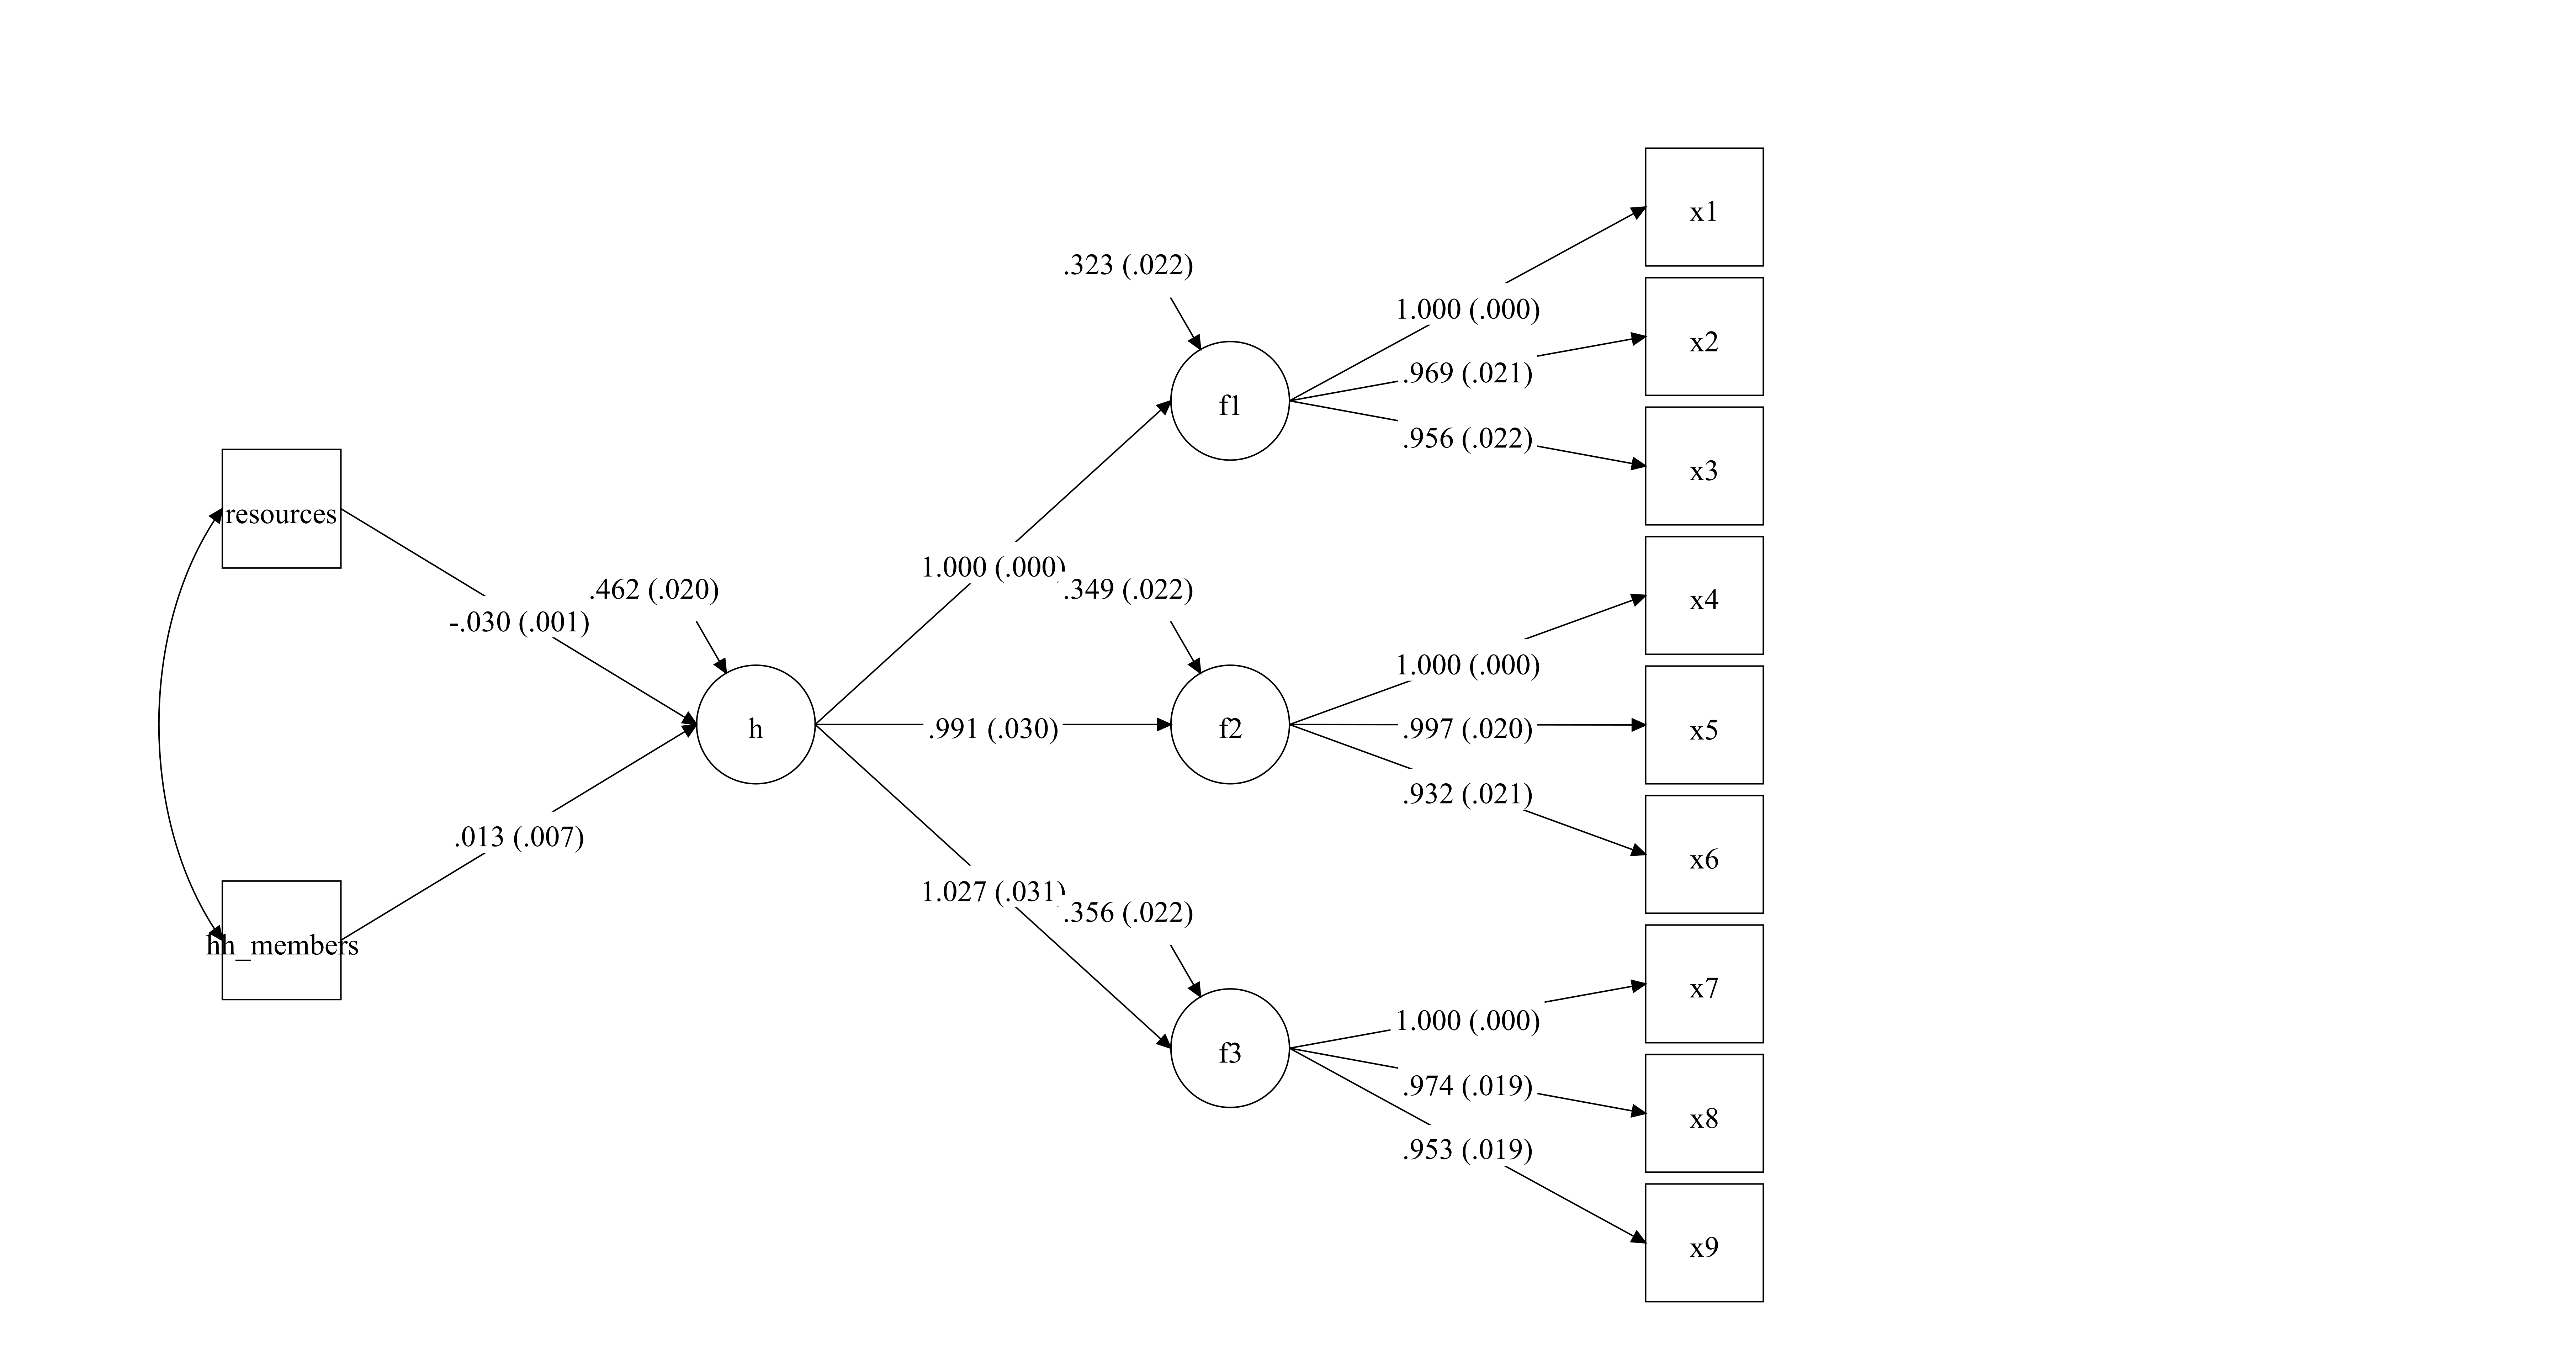
\includegraphics[width=\textwidth]{val_sem_1} \caption{This is a MIMIC model were a higher-order factor model loads into three dimensions and there is one path to examine criterion validity (resources and hh members)}\label{fig:valsem1}
\end{figure}

\hypertarget{real-data-example-1}{%
\subsection{Real-data example}\label{real-data-example-1}}

We will use the Mexican data (pobreza\_14.dta) to illustrate how validity could be assessed using a MIMIC model. We had already created a *.dat file (Mex\_pobreza\_14.dat) with the variables we need for the analysis (Section ). We can inspect the deprivation variables to familiarise ourselves with these data. The reduce model of the Mexican multidimensional measure comprises 14 variables classified in three dimensions: Housing, Essential services and food deprivation.

\begin{Shaded}
\begin{Highlighting}[]
\KeywordTok{library}\NormalTok{(haven)}
\NormalTok{Mex_D<-}\KeywordTok{read_dta}\NormalTok{(}\StringTok{"pobreza_14.dta"}\NormalTok{)}
\KeywordTok{head}\NormalTok{(Mex_D[}\DecValTok{31}\OperatorTok{:}\DecValTok{34}\NormalTok{])}
\end{Highlighting}
\end{Shaded}

\begin{verbatim}
## # A tibble: 6 x 4
##            icv_muros          icv_techos         icv_pisos          icv_hac
##            <dbl+lbl>           <dbl+lbl>         <dbl+lbl>        <dbl+lbl>
## 1 0 [No presenta ca~ 0 [No presenta car~ 0 [No presenta c~ 0 [No presenta ~
## 2 0 [No presenta ca~ 0 [No presenta car~ 0 [No presenta c~ 0 [No presenta ~
## 3 0 [No presenta ca~ 0 [No presenta car~ 0 [No presenta c~ 0 [No presenta ~
## 4 0 [No presenta ca~ 0 [No presenta car~ 0 [No presenta c~ 0 [No presenta ~
## 5 0 [No presenta ca~ 0 [No presenta car~ 0 [No presenta c~ 0 [No presenta ~
## 6 0 [No presenta ca~ 0 [No presenta car~ 0 [No presenta c~ 0 [No presenta ~
\end{verbatim}

\begin{Shaded}
\begin{Highlighting}[]
\KeywordTok{head}\NormalTok{(Mex_D[}\DecValTok{36}\OperatorTok{:}\DecValTok{39}\NormalTok{])}
\end{Highlighting}
\end{Shaded}

\begin{verbatim}
## # A tibble: 6 x 4
##             isb_agua           isb_dren          isb_luz         isb_combus
##            <dbl+lbl>          <dbl+lbl>        <dbl+lbl>          <dbl+lbl>
## 1 0 [No presenta ca~ 0 [No presenta ca~ 0 [No presenta ~ 0 [No presenta ca~
## 2 0 [No presenta ca~ 0 [No presenta ca~ 0 [No presenta ~ 0 [No presenta ca~
## 3 0 [No presenta ca~ 0 [No presenta ca~ 0 [No presenta ~ 0 [No presenta ca~
## 4 0 [No presenta ca~ 0 [No presenta ca~ 0 [No presenta ~ 0 [No presenta ca~
## 5 0 [No presenta ca~ 0 [No presenta ca~ 0 [No presenta ~ 0 [No presenta ca~
## 6 0 [No presenta ca~ 0 [No presenta ca~ 0 [No presenta ~ 0 [No presenta ca~
\end{verbatim}

\begin{Shaded}
\begin{Highlighting}[]
\KeywordTok{head}\NormalTok{(Mex_D[}\DecValTok{41}\OperatorTok{:}\DecValTok{46}\NormalTok{])}
\end{Highlighting}
\end{Shaded}

\begin{verbatim}
## # A tibble: 6 x 6
##   ia_1ad ia_2ad ia_3ad ia_4ad ia_5ad ia_6ad
##    <dbl>  <dbl>  <dbl>  <dbl>  <dbl>  <dbl>
## 1      1      1      1      1      1      0
## 2      0      0      0      0      0      0
## 3      1      0      0      0      0      0
## 4      0      0      0      0      0      0
## 5      0      0      0      0      0      0
## 6      1      1      1      0      1      0
\end{verbatim}

For the validity analysis we will fit the same higher-order CFA model with the three dimensions (essential services, housing quality and food deprivation). We will use two validators: Education attainment of the household head and an index of assets (fridge, tv, washing machine, computer and internet). The estimation of the parameters of both validators will be adjusted by rural v urban areas (rururb) and household size (tot\_integ).

We will fit the model on Mplus. We will add the four new variables to the USEVARIABLES list and then include four new paths to the CFA model. This is achieved by including ``h on rururb tot\_integ durables educ\_hh;'' in the script (val\_CFA\_mex.inp). Again, we will save this in the test object and we will run the model from R using the \texttt{mplusModeler()} function. Bear in mind that the model will take some seconds to run.

\begin{Shaded}
\begin{Highlighting}[]
\NormalTok{test <-}\StringTok{ }\KeywordTok{mplusObject}\NormalTok{(}
\DataTypeTok{TITLE =} \StringTok{"Validity Mexico CFA model;"}\NormalTok{,}
   \DataTypeTok{VARIABLE =} \StringTok{"}
\StringTok{     NAMES = proyecto folioviv foliohog icv_muros icv_techos}
\StringTok{             icv_pisos icv_hac isb_agua isb_dren isb_luz isb_combus}
\StringTok{             ic_sbv ia_1ad ia_2ad ia_3ad ia_4ad ia_5ad ia_6ad}
\StringTok{             ia_7men ia_8men ia_9men ia_10men ia_11men ia_12men}
\StringTok{             tv_dep radio_dep fridge_dep}
\StringTok{             washingmach_dep compu_dep inter_dep psu weight}
\StringTok{             rururb tot_integ durables educ_hh;}
\StringTok{MISSING=.;}
\StringTok{     CATEGORICAL = icv_muros icv_techos icv_pisos icv_hac isb_agua}
\StringTok{                   isb_dren isb_luz isb_combus  ia_1ad}
\StringTok{                   ia_2ad ia_3ad ia_4ad ia_5ad ia_6ad;}
\StringTok{     USEVARIABLES = icv_muros icv_techos icv_pisos icv_hac isb_agua}
\StringTok{                   isb_dren isb_luz isb_combus  ia_1ad}
\StringTok{                   ia_2ad ia_3ad ia_4ad ia_5ad ia_6ad}
\StringTok{                   rururb tot_integ durables educ_hh;}

\StringTok{WEIGHT=weight;}
\StringTok{cluster = psu;"}\NormalTok{,}

   \DataTypeTok{ANALYSIS =} \StringTok{"TYPE = complex;}

\StringTok{ESTIMATOR = wlsmv;}
\StringTok{PROCESS = 4;"}\NormalTok{,}

\DataTypeTok{MODEL =} \StringTok{"f1 by icv_muros icv_techos icv_pisos icv_hac;}
\StringTok{  f2 by isb_agua}
\StringTok{        isb_dren isb_luz isb_combus;}
\StringTok{  f3 by ia_1ad ia_2ad ia_3ad ia_4ad ia_5ad ia_6ad;}
\StringTok{  h  by f1 f2 f3;}
\StringTok{  h on durables educ_hh rururb tot_integ;"}\NormalTok{,}

\DataTypeTok{OUTPUT =} \StringTok{"std stdyx;"}\NormalTok{)}

\NormalTok{res<-}\KeywordTok{mplusModeler}\NormalTok{(test, }\DataTypeTok{modelout =} \StringTok{"val_CFA_mex.inp"}\NormalTok{,}
                    \DataTypeTok{writeData =} \StringTok{"never"}\NormalTok{, }\DataTypeTok{hashfilename =} \OtherTok{FALSE}\NormalTok{,}
                    \DataTypeTok{dataout=}\StringTok{"Mex_pobreza_14.dat"}\NormalTok{, }\DataTypeTok{run =}\NormalTok{ 1L)}
\end{Highlighting}
\end{Shaded}

\begin{verbatim}
## Wrote model to: val_CFA_mex.inp
\end{verbatim}

\begin{verbatim}
## Wrote data to: Mex_pobreza_14.dat
\end{verbatim}

\begin{verbatim}
## No action taken as writeData = 'never'
\end{verbatim}

\begin{verbatim}
## 
## Running model: val_CFA_mex.inp 
## System command: C:\WINDOWS\system32\cmd.exe /c cd "." && "Mplus" "val_CFA_mex.inp" 
## Reading model:  val_CFA_mex.out
\end{verbatim}

Once the model has been fitted we can examine construct validity by assessing whether our model holds after adding the predictors. We will save the statistics of fit in the \texttt{fitstats()} object. We can see that the fit of this model is very good. We find that the model seems to be a valid representation of poverty for Mexico. That means that the dimensions and indicators are adequately classified and identified.

\begin{Shaded}
\begin{Highlighting}[]
\NormalTok{fitstats<-}\KeywordTok{c}\NormalTok{(}\DataTypeTok{TLI=}\NormalTok{res}\OperatorTok{$}\NormalTok{results}\OperatorTok{$}\NormalTok{summaries}\OperatorTok{$}\NormalTok{TLI,}
            \DataTypeTok{CFI=}\NormalTok{res}\OperatorTok{$}\NormalTok{results}\OperatorTok{$}\NormalTok{summaries}\OperatorTok{$}\NormalTok{CFI,}
            \DataTypeTok{Chisq=}\NormalTok{res}\OperatorTok{$}\NormalTok{results}\OperatorTok{$}\NormalTok{summaries}\OperatorTok{$}\NormalTok{ChiSqM_PValue,}
            \DataTypeTok{RMSEA=}\NormalTok{res}\OperatorTok{$}\NormalTok{results}\OperatorTok{$}\NormalTok{summaries}\OperatorTok{$}\NormalTok{RMSEA_Estimate)}
\NormalTok{fitstats}
\end{Highlighting}
\end{Shaded}

\begin{verbatim}
##   TLI   CFI Chisq RMSEA 
## 0.987 0.989 0.000 0.019
\end{verbatim}

On Mplus we can produce a diagram to display the estimated values of the parameters of our model. From left to right, we appreciate the standardised parameters of the validators and the adjustment variables. We see the four have the expected signs. The higher the education attainment, the lower the factor scores (higher severity). The asset index shows a similar behaviour, having more durables in the household is associated with lower factor scores. Both rurality and the household size increase the factor scores. Then we appreciate that the standardised factor loadings are high (\(>.5\)).

\begin{figure}[H]

{\centering 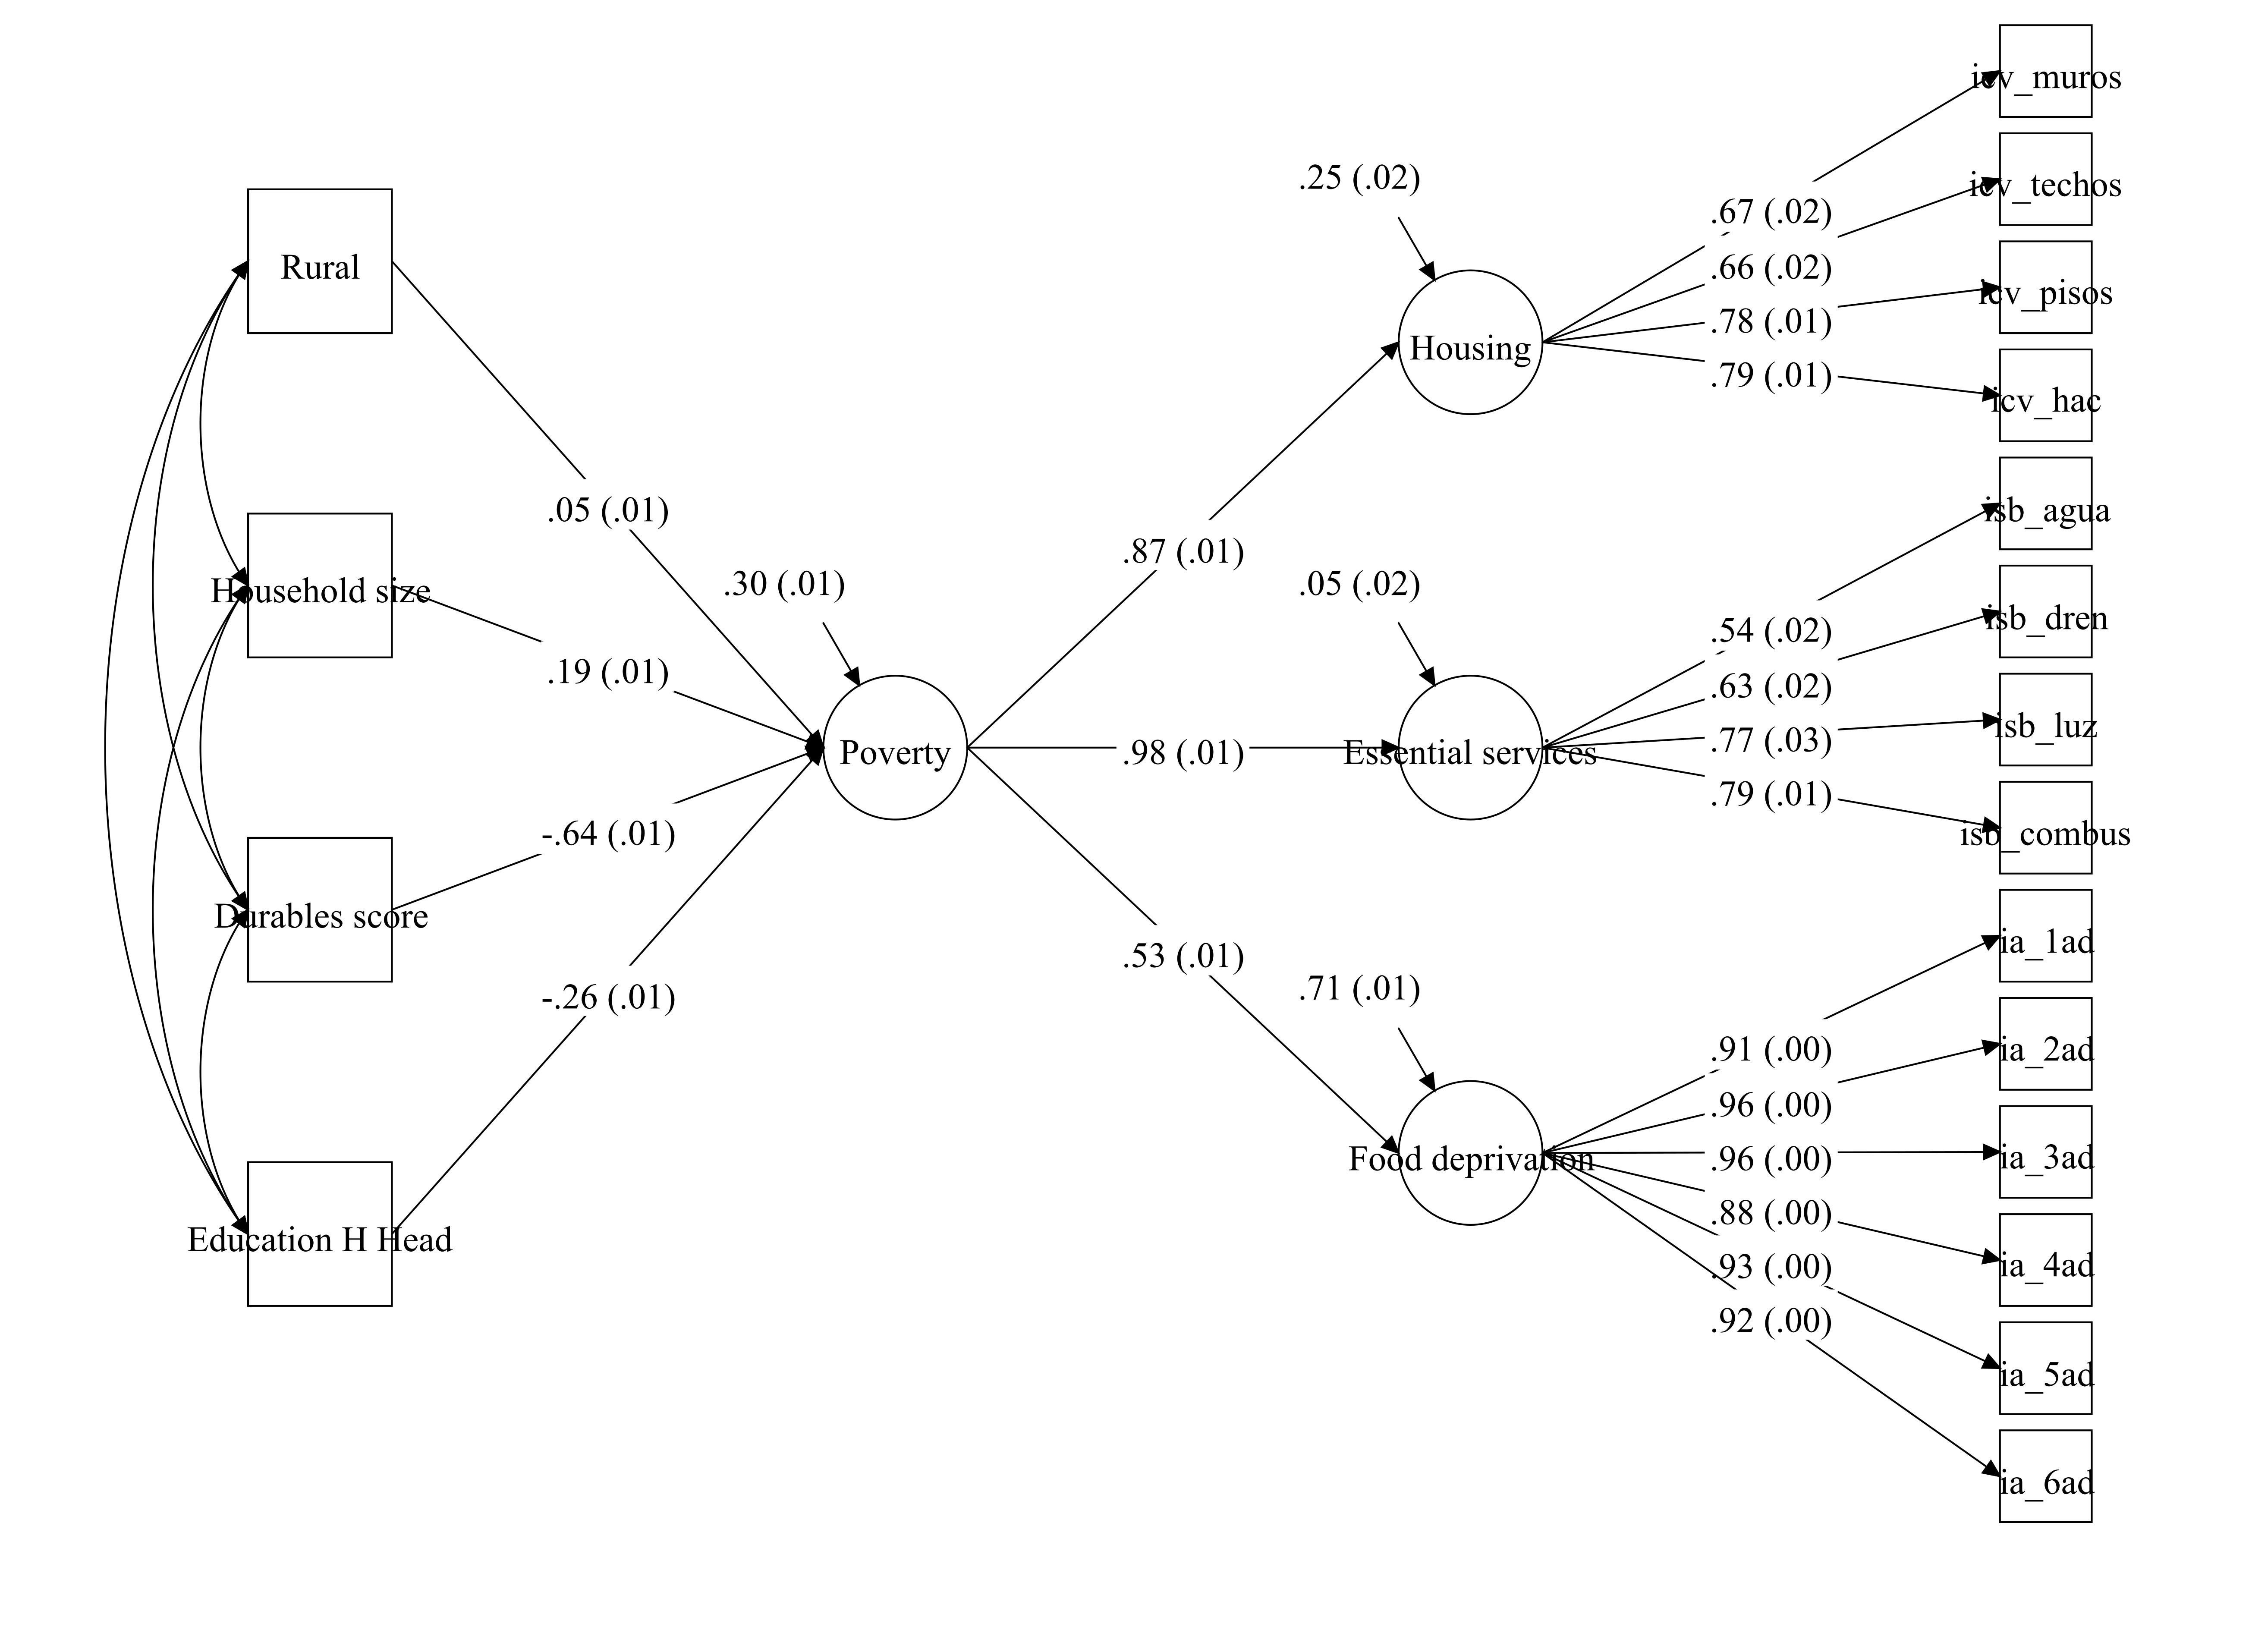
\includegraphics[width=\textwidth]{val_cfa_mex} 

}

\caption{This is a MIMIC model of a reduced version of the multidimensional Mexican measure. The model shows that poverty is associated by possession of different goods and education attainment of the household head, adjusted by rurality and household size. Standardised coefficients (Standard error within brackets)}\label{fig:valcfamex}
\end{figure}

\hypertarget{Chapter-5}{%
\chapter{Comparability in poverty measurement}\label{Chapter-5}}

\textbf{Abstract}

This chapter discusses the problem of comparability in poverty measurement and frames this challenge using the principle of measurement invariance. The chapter provides an intuitive explanation of measurement invariance. A connection between measurement invariance, validity and reliability is provided. Then the chapter uses simulated data to illustrate how measurement invariance works and how can it be analysed in Mplus. The chapter also provides a real-data example.

\hypertarget{measurement-invariance}{%
\section{Measurement invariance}\label{measurement-invariance}}

Making comparisons of poverty across time or units (countries, regions, population groups) is one of the chief goals in poverty research. Ideally, changes in poverty from a given year to another must reflect effective changes in living standards. The same must hold when comparing estimates across groups where poverty must be relatively higher or lower given differences in living standards across the units of interest. Nonetheless, survey data is subject to different kinds of amendments overtime. There are changes to the questionnaire that aim to update poverty indices, researchers also include or exclude different indicators overtime and across groups, data collection modes and sampling frameworks might differ. These modifications are likely to affect the comparability of poverty estimates overtime or across countries using similar data.

In poverty measurement the literature often proposes that if one has the same indicators, poverty is being measured on equivalent terms. MI transforms this proposition into an assumption as there is no guarantee that using the same indicators measure poverty on the same terms. There are several survey and non-survey aspects affecting the full comparability of poverty indices: sampling framework, data-collection mode (face to face, computer-based, telephone, etc.), different survey questionnaires, changes in living standards that result between-unit reliability and validity discrepancies (i.e.~some items or dimensions might be highly reliable to measure poverty in one group but not in other). The effect of these issues could be so high upon comparability than just using the same indicators to contrast the severity and prevalence of poverty across groups or time is unlikely to be enough.

The concern with the quantifying the effect of the different sources of incompatibility and disparity of different indices pushed measurement theory to develop a framework to conceptualise and then empirically assess comparability across measures. The rationale of factor analysis - the existent of a measurement model for a population- was extended to assess the extent to which different indices are comparable or not. This has resulted in the development of the concept of measurement invariance (MI) which defines comparability in terms of the extent to which a factor model holds for different populations {[}Meredith (\protect\hyperlink{ref-Meredith1993}{1993});Meredith \& Teresi (\protect\hyperlink{ref-Meredith2006}{2006});Schoot, Lugtig, \& Hox (\protect\hyperlink{ref-Schoot2012}{2012});Lubke, Dolan, Kelderman, \& Mellenbergh (\protect\hyperlink{ref-Lubke2003}{2003});Byrne, Shavelson, \& Muthén (\protect\hyperlink{ref-Byrne1989}{1989})\}. That means that the structure of a poverty index (dimensions and items), the relationship between the indicators and the latent construct and the error term are similar across periods or groups. That is, having two poverty indices with the same indicators is not a sufficient to make meaningful comparisons of the prevalence and severity of poverty across groups. Therefore, Measurement Invariance (MI) is a necessary condition for making comparisons of subjects using a given index. Formally, MI can be defined as the capacity of an index to measure equivalently across two or more groups or periods.

MI implies that deprivation should change equally across two groups after the level of poverty of two groups changes in the same order of magnitude. In contrast, when MI is violated, it means that one group is being unfairly compared against another because there is another phenomenon causing the change in deprivation. This is a very undesirable feature of a poverty index because it would mean that the differences in prevalence and severity are due to different sources that are not related with poverty. Researchers cannot conclude that poverty is higher/lower given that the discrepancies are explained by sampling differences, data collection modes, dissimilar questionnaires, acute between-group differences reliability and validity.

MI is an ideal preposition and it could be violated in different ways. There are diverse aspects of MI that can be assessed and translated into the following standards (Meredith, \protect\hyperlink{ref-Meredith1993}{1993}).

\begin{itemize}
\tightlist
\item
  Strict MI: This is the ideal level of MI as the structure, the relationship of the items with the latent variable, the indicator means and the residuals are equivalent across groups/periods.
\item
  Strong MI: The structure, the relationship of the items with the latent variable and the indicator means are invariant across groups/periods.
\item
  Weak MI: The structure and the relationship of the items with the construct are equivalent.
\item
  Configural MI: Only the structure is the same across groups/periods.
\end{itemize}

\hypertarget{introduction-to-key-aspects-of-measurement-invariance}{%
\section{Introduction to key aspects of measurement invariance}\label{introduction-to-key-aspects-of-measurement-invariance}}

Measurement invariance is, therefore, about the similarity of the different parameters of a latent variable model across different groups. To introduce the notion of MI, simulated data was generated for 20 groups. In the simplest case, a unidimensional model is proposed where poverty is measured using 15 binary indicators. To make clearer what could happen when MI is violated, the parameters of five indicators where changed for half of the groups. This poses a situation where the poverty indices across 20 groups (e.g.~countries) have the same structure -Configural Invariance- but there are substantive differences in the way in which some indicators capture poverty across units.

A two Item Response Theory (IRT) model was fitted to the simulated data to estimate both discrimination (\(a\)) and severity (\(b\)) parameters for each group. The models were fitted on Mplus 7.2 using the following code and the R-package MplusAutomation (Hallquist \& Wiley, \protect\hyperlink{ref-Hallquist2018}{2018}).

\begin{verbatim}
[[init]]
iterators = i j;
i = 1:10;
j = 1:2;
filename = IRT_[[j]]_[[i]].inp;

outputDirectory = "C:../PM Book";

[[/init]]
DATA : FILE = UD_data_[[j]]_[[i]].dat;

VARIABLE : NAMES=V1-V15; 
           USEVARIABLES=V1-V15; 
           CATEGORICAL = V1-V15;
           
MODEL: f by V1-V15*;
       f@1;
\end{verbatim}

\begin{Shaded}
\begin{Highlighting}[]
\CommentTok{## Running the IRT using the Mplusautomation package ##}

\CommentTok{#createModels("IRT_models_MI_Section.txt")}
\CommentTok{#runModels(filefilter = "MI_IRT_")}

\CommentTok{#Importing the *.out from mplus into R#}

\NormalTok{irt_MI<-}\KeywordTok{readModels}\NormalTok{(}\DataTypeTok{filefilter =}\StringTok{"mi_irt_"}\NormalTok{)}

\CommentTok{#Putting both parameters into a list#}

\NormalTok{irt_MI<-}\KeywordTok{lapply}\NormalTok{(irt_MI, }\ControlFlowTok{function}\NormalTok{(x) \{}
\NormalTok{  x<-x}\OperatorTok{$}\NormalTok{parameters}\OperatorTok{$}\NormalTok{irt.parameterization}
\NormalTok{  x<-x[}\DecValTok{1}\OperatorTok{:}\DecValTok{30}\NormalTok{,]}
\NormalTok{  x<-}\KeywordTok{data.frame}\NormalTok{(}\DataTypeTok{a=}\NormalTok{x}\OperatorTok{$}\NormalTok{est[}\DecValTok{1}\OperatorTok{:}\DecValTok{15}\NormalTok{],}\DataTypeTok{b=}\NormalTok{x}\OperatorTok{$}\NormalTok{est[}\DecValTok{16}\OperatorTok{:}\DecValTok{30}\NormalTok{])}
\NormalTok{  x}
\NormalTok{\}}
\NormalTok{)}
\end{Highlighting}
\end{Shaded}

We inspect the first object in list \texttt{irt\textbackslash{}\_MI} and check the values of both discrimination (a) and severity (b) for the 15 items. The items have increasing discrimination values.

\begin{Shaded}
\begin{Highlighting}[]
\NormalTok{irt_MI[[}\DecValTok{1}\NormalTok{]]}
\end{Highlighting}
\end{Shaded}

\begin{verbatim}
##        a     b
## 1  0.667 2.905
## 2  0.861 2.292
## 3  0.791 2.510
## 4  0.911 2.340
## 5  0.981 1.586
## 6  1.167 1.126
## 7  1.214 0.871
## 8  1.301 0.651
## 9  1.285 0.457
## 10 1.363 0.724
## 11 1.405 0.677
## 12 1.437 0.698
## 13 1.473 0.427
## 14 1.564 0.287
## 15 1.699 0.197
\end{verbatim}

The list has 20 objects it is possible to create a data frame using few lines of code so that we can plot and inspect how the estimates vary across groups.

\begin{Shaded}
\begin{Highlighting}[]
\CommentTok{#Load this packages if necessary}
\KeywordTok{library}\NormalTok{(ggplot2)}
\KeywordTok{library}\NormalTok{(reshape2)}

\CommentTok{#Creating a data frame to plot the parameters by group}
\NormalTok{irt_MI<-}\KeywordTok{as.data.frame}\NormalTok{(irt_MI)}
\NormalTok{irt_MI}\OperatorTok{$}\NormalTok{var_id<-}\DecValTok{1}\OperatorTok{:}\DecValTok{15}
\end{Highlighting}
\end{Shaded}

The values of both parameters for group 1 and 10 can be inspected using the following code. It is clear that there are very little deviation from one group to another. This is an indication than strong MI might hold between these two groups as both loadings (discrimination) and thresholds (severity) are similar between group 1 and 10. However, the interest is to assess whether the parameters change dramatically across groups.

\begin{Shaded}
\begin{Highlighting}[]
\NormalTok{irt_MI[}\DecValTok{1}\OperatorTok{:}\DecValTok{15}\NormalTok{,}\DecValTok{1}\OperatorTok{:}\DecValTok{4}\NormalTok{]}
\end{Highlighting}
\end{Shaded}

\begin{verbatim}
##    mi_irt_1_1.out.a mi_irt_1_1.out.b mi_irt_1_10.out.a mi_irt_1_10.out.b
## 1             0.667            2.905             0.676             2.875
## 2             0.861            2.292             0.738             2.470
## 3             0.791            2.510             0.799             2.566
## 4             0.911            2.340             0.905             2.353
## 5             0.981            1.586             0.982             1.590
## 6             1.167            1.126             1.101             1.152
## 7             1.214            0.871             1.099             0.906
## 8             1.301            0.651             1.254             0.646
## 9             1.285            0.457             1.268             0.426
## 10            1.363            0.724             1.361             0.692
## 11            1.405            0.677             1.373             0.658
## 12            1.437            0.698             1.467             0.649
## 13            1.473            0.427             1.449             0.356
## 14            1.564            0.287             1.610             0.253
## 15            1.699            0.197             1.560             0.169
\end{verbatim}

Then we can rearrange the data to produce the plots to make a visual inspection of the parameters.

\begin{Shaded}
\begin{Highlighting}[]
\NormalTok{irt_MI<-}\KeywordTok{melt}\NormalTok{(irt_MI, }\DataTypeTok{id=}\StringTok{"var_id"}\NormalTok{)}
\NormalTok{irt_MI}\OperatorTok{$}\NormalTok{variable<-}\KeywordTok{sub}\NormalTok{(}\StringTok{'.*(?=.$)'}\NormalTok{, }\StringTok{''}\NormalTok{, irt_MI}\OperatorTok{$}\NormalTok{variable, }\DataTypeTok{perl=}\NormalTok{T)}
\NormalTok{irt_MI}\OperatorTok{$}\NormalTok{data<-}\KeywordTok{rep}\NormalTok{(}\DecValTok{1}\OperatorTok{:}\DecValTok{20}\NormalTok{,}\DataTypeTok{each=}\DecValTok{30}\NormalTok{)}

\NormalTok{irt_MIa_mi<-}\KeywordTok{subset}\NormalTok{(irt_MI,irt_MI}\OperatorTok{$}\NormalTok{variable}\OperatorTok{==}\StringTok{"a"} \OperatorTok{&}\StringTok{ }\NormalTok{irt_MI}\OperatorTok{$}\NormalTok{var_id}\OperatorTok{>=}\DecValTok{5}\NormalTok{)}
\NormalTok{irt_MIa_nonmi<-}\KeywordTok{subset}\NormalTok{(irt_MI,irt_MI}\OperatorTok{$}\NormalTok{variable}\OperatorTok{==}\StringTok{"a"} \OperatorTok{&}\StringTok{ }\NormalTok{irt_MI}\OperatorTok{$}\NormalTok{var_id}\OperatorTok{<}\DecValTok{5}\NormalTok{)}

\NormalTok{irt_MIb_mi<-}\KeywordTok{subset}\NormalTok{(irt_MI,irt_MI}\OperatorTok{$}\NormalTok{variable}\OperatorTok{==}\StringTok{"b"} \OperatorTok{&}\StringTok{ }\NormalTok{irt_MI}\OperatorTok{$}\NormalTok{var_id}\OperatorTok{>=}\DecValTok{5}\NormalTok{)}
\NormalTok{irt_MIb_nonmi<-}\KeywordTok{subset}\NormalTok{(irt_MI,irt_MI}\OperatorTok{$}\NormalTok{variable}\OperatorTok{==}\StringTok{"b"} \OperatorTok{&}\StringTok{ }\NormalTok{irt_MI}\OperatorTok{$}\NormalTok{var_id}\OperatorTok{<}\DecValTok{5}\NormalTok{)}
\end{Highlighting}
\end{Shaded}

Figure \ref{fig:MIhodls1} plots the discrimination parameters of each group that are likely -we say likely because below MI is formally tested- to be invariant across the 20 groups. There are small fluctuation from one group to another, indicating that changes in poverty produce similar changes in deprivation of the item in question across groups. As discussed in Chapter 4 (Reliability), this parameter can be used to assess monotonicity. Figure \ref{fig:MInothodls1} plots the discrimination parameters for the first five items (1 to 5). For the first 10 groups the fluctuation is small. However, we can appreciate that for the other 10 groups, the discrimination parameters are very different. This is an indication that MI might not hold between two clusters of groups (1-10 and 11-20). The discrimination values in plot 5.2 suggest that a change in poverty result in less dramatic changes in deprivation for the first ten groups. If these five indicators were exclusively used to measure poverty, some groups will be highly disfavoured relative to the others as there is something else (not only poverty) causing changes in observed deprivation. In the next section the discussion is enriched by using a real data example.

\begin{Shaded}
\begin{Highlighting}[]
\KeywordTok{ggplot}\NormalTok{(irt_MIa_mi,}\KeywordTok{aes}\NormalTok{(}\DataTypeTok{x=}\NormalTok{data,}\DataTypeTok{y=}\NormalTok{value,}\DataTypeTok{group=}\NormalTok{var_id)) }\OperatorTok{+}\StringTok{ }\KeywordTok{geom_point}\NormalTok{()  }\OperatorTok{+}\StringTok{ }
\StringTok{  }\KeywordTok{geom_line}\NormalTok{(}\KeywordTok{aes}\NormalTok{(}\DataTypeTok{linetype=}\KeywordTok{as.factor}\NormalTok{(var_id))) }\OperatorTok{+}\StringTok{ }
\StringTok{  }\KeywordTok{xlab}\NormalTok{(}\StringTok{"Groups 1-20"}\NormalTok{) }\OperatorTok{+}\StringTok{ }\KeywordTok{ylab}\NormalTok{(}\StringTok{"Discrimination parameter. IRT scale"}\NormalTok{) }\OperatorTok{+}\StringTok{ }
\StringTok{  }\KeywordTok{labs}\NormalTok{(}\DataTypeTok{linetype=}\StringTok{'Indicator id'}\NormalTok{) }\OperatorTok{+}\StringTok{  }
\StringTok{  }\KeywordTok{scale_y_continuous}\NormalTok{( }\DataTypeTok{limits =} \KeywordTok{c}\NormalTok{(.}\DecValTok{5}\NormalTok{,}\DecValTok{2}\NormalTok{), }\DataTypeTok{expand =} \KeywordTok{c}\NormalTok{(}\DecValTok{0}\NormalTok{,}\DecValTok{0}\NormalTok{), }\DataTypeTok{breaks =} \KeywordTok{seq}\NormalTok{(.}\DecValTok{5}\NormalTok{, }\DecValTok{2}\NormalTok{, }\FloatTok{.25}\NormalTok{) ) }\OperatorTok{+}\StringTok{ }
\StringTok{  }\KeywordTok{theme_bw}\NormalTok{() }
\end{Highlighting}
\end{Shaded}

\begin{figure}
\centering
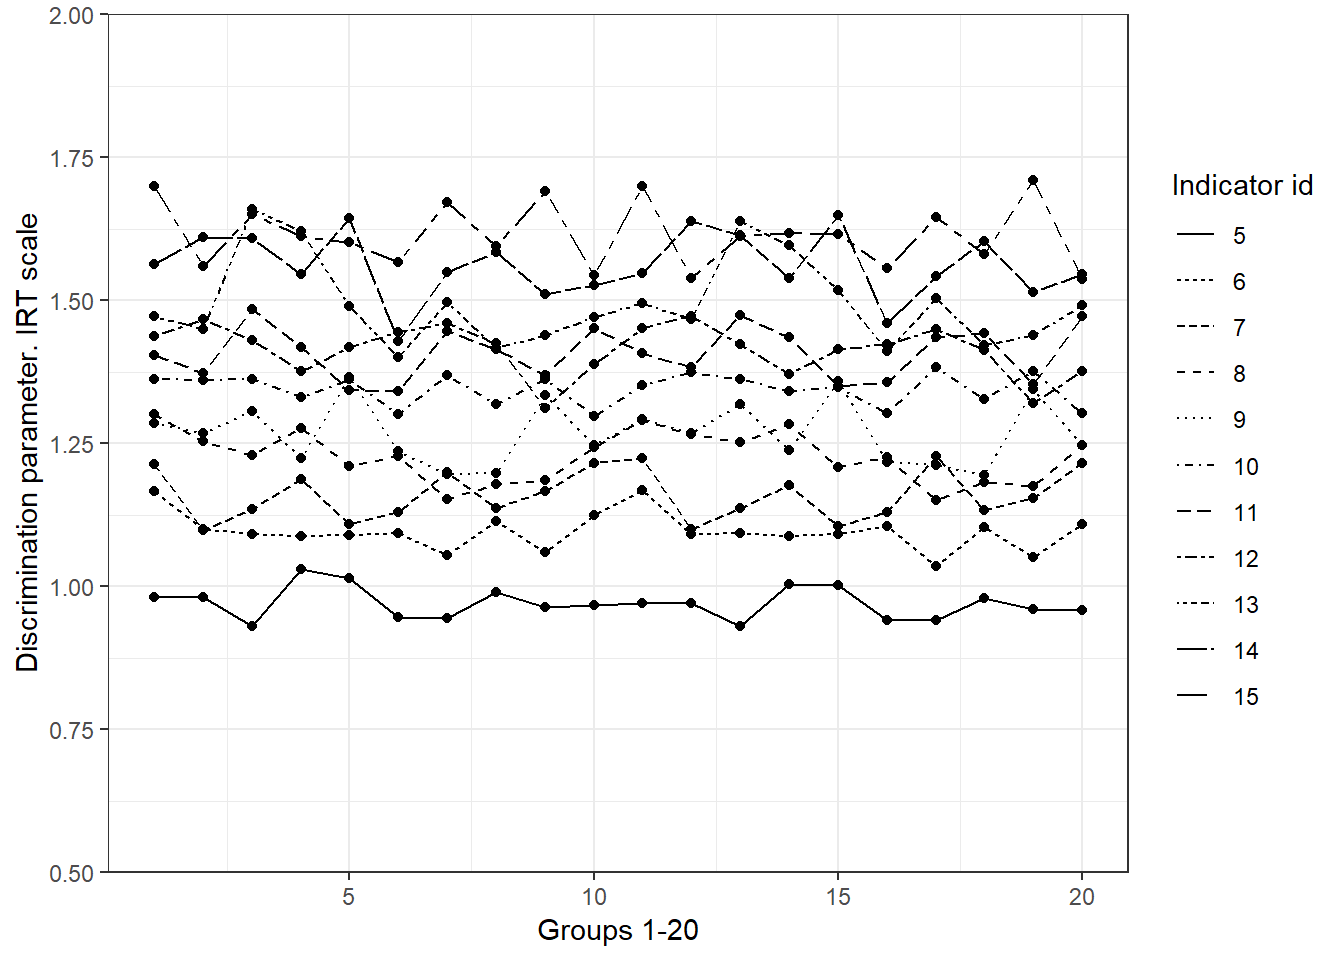
\includegraphics{PM_Book_files/figure-latex/MIhodls1-1.png}
\caption{\label{fig:MIhodls1}Discrimination parameters that seem to fulfil MI. Simulated data. We see very little fluctuation from one group to another}
\end{figure}

\begin{Shaded}
\begin{Highlighting}[]
\KeywordTok{ggplot}\NormalTok{(irt_MIa_nonmi,}\KeywordTok{aes}\NormalTok{(}\DataTypeTok{x=}\NormalTok{data,}\DataTypeTok{y=}\NormalTok{value,}\DataTypeTok{group=}\NormalTok{var_id)) }\OperatorTok{+}\StringTok{ }\KeywordTok{geom_point}\NormalTok{()  }\OperatorTok{+}\StringTok{ }
\StringTok{  }\KeywordTok{geom_line}\NormalTok{(}\KeywordTok{aes}\NormalTok{(}\DataTypeTok{linetype=}\KeywordTok{as.factor}\NormalTok{(var_id))) }\OperatorTok{+}\StringTok{ }
\StringTok{  }\KeywordTok{xlab}\NormalTok{(}\StringTok{"Groups 1-20"}\NormalTok{) }\OperatorTok{+}\StringTok{ }\KeywordTok{ylab}\NormalTok{(}\StringTok{"Discrimination parameter. IRT scale"}\NormalTok{) }\OperatorTok{+}\StringTok{ }
\StringTok{  }\KeywordTok{labs}\NormalTok{(}\DataTypeTok{linetype=}\StringTok{'Indicator id'}\NormalTok{) }\OperatorTok{+}\StringTok{  }
\StringTok{  }\KeywordTok{scale_y_continuous}\NormalTok{( }\DataTypeTok{limits =} \KeywordTok{c}\NormalTok{(.}\DecValTok{5}\NormalTok{,}\DecValTok{2}\NormalTok{), }\DataTypeTok{expand =} \KeywordTok{c}\NormalTok{(}\DecValTok{0}\NormalTok{,}\DecValTok{0}\NormalTok{), }\DataTypeTok{breaks =} \KeywordTok{seq}\NormalTok{(.}\DecValTok{5}\NormalTok{, }\DecValTok{2}\NormalTok{, }\FloatTok{.25}\NormalTok{) ) }\OperatorTok{+}\StringTok{ }
\StringTok{  }\KeywordTok{theme_bw}\NormalTok{() }
\end{Highlighting}
\end{Shaded}

\begin{figure}
\centering
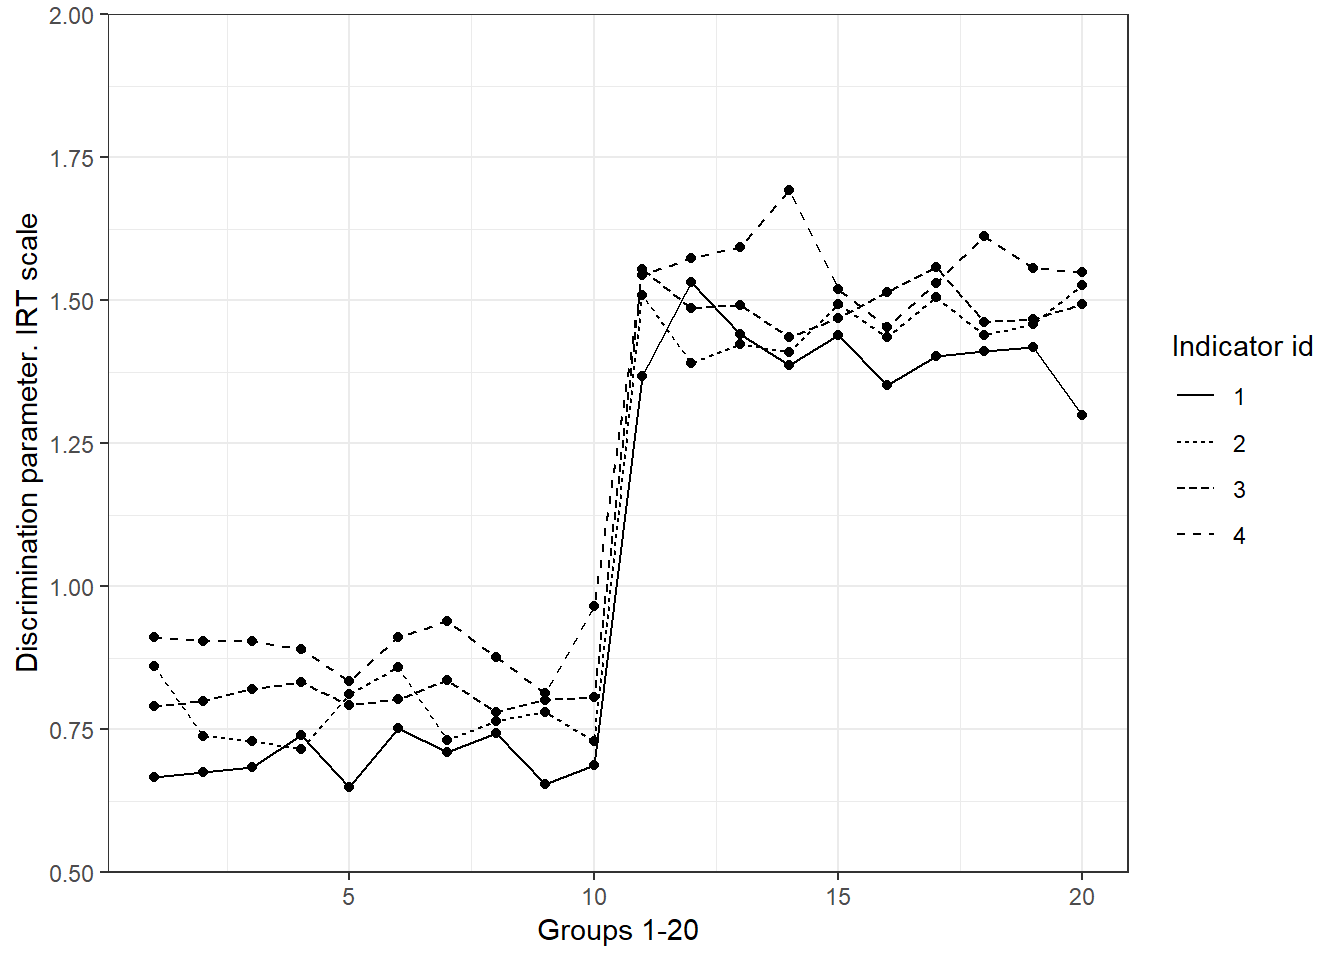
\includegraphics{PM_Book_files/figure-latex/MInothodls1-1.png}
\caption{\label{fig:MInothodls1}Discrimination parameters that do not seem to fulfil MI. Simulated data. We see a lot of fluctuation from groups 11-20 relative to 1-10}
\end{figure}

Figures \ref{fig:MIhodls2} and 5.4 plot the values of the severity parameter for the items that are likely to be invariant across all groups and for the items that seem to violate MI, respectively. The severity parameters range between 0 and 3 standard deviations. As discussed in Chapter 4, this is the expected behaviour when looking at low standard of living. The items in plot \ref{fig:MIhodls2} are very stable across groups. In contrast the severity parameters change a lot for groups 11 to 20 in comparison with the first ten groups (Figure \ref{fig:MInothodls2}). It seems, therefore, that these items are non-invariant, at least, between these two clusters. The severity parameter is tied with the intercept of a factor model (See Chapter 4). It indicates the mean value of deprivation for each item given the latent value of poverty. Different means are a violation of strong MI, and therefore is undesirable. In poverty research indicates the case where an indicator is a more/less severe manifestation of poverty when comparing two or more groups. In other words, it is an indication of when an indicator of a given society might be too severe to measure poverty in another. This is explained further using the real data example.

\begin{Shaded}
\begin{Highlighting}[]
\KeywordTok{ggplot}\NormalTok{(irt_MIb_mi,}\KeywordTok{aes}\NormalTok{(}\DataTypeTok{x=}\NormalTok{data,}\DataTypeTok{y=}\NormalTok{value,}\DataTypeTok{group=}\NormalTok{var_id)) }\OperatorTok{+}\StringTok{ }\KeywordTok{geom_point}\NormalTok{()  }\OperatorTok{+}\StringTok{ }
\StringTok{  }\KeywordTok{geom_line}\NormalTok{(}\KeywordTok{aes}\NormalTok{(}\DataTypeTok{linetype=}\KeywordTok{as.factor}\NormalTok{(var_id))) }\OperatorTok{+}\StringTok{ }
\StringTok{  }\KeywordTok{xlab}\NormalTok{(}\StringTok{"Groups 1-20"}\NormalTok{) }\OperatorTok{+}\StringTok{ }\KeywordTok{ylab}\NormalTok{(}\StringTok{"Severity parameter. IRT scale"}\NormalTok{) }\OperatorTok{+}\StringTok{ }
\StringTok{  }\KeywordTok{labs}\NormalTok{(}\DataTypeTok{linetype=}\StringTok{'Indicator id'}\NormalTok{) }\OperatorTok{+}\StringTok{  }
\StringTok{  }\KeywordTok{scale_y_continuous}\NormalTok{( }\DataTypeTok{limits =} \KeywordTok{c}\NormalTok{(}\DecValTok{0}\NormalTok{,}\DecValTok{4}\NormalTok{), }\DataTypeTok{expand =} \KeywordTok{c}\NormalTok{(}\DecValTok{0}\NormalTok{,}\DecValTok{0}\NormalTok{), }\DataTypeTok{breaks =} \KeywordTok{seq}\NormalTok{(}\DecValTok{0}\NormalTok{, }\DecValTok{4}\NormalTok{, }\FloatTok{.5}\NormalTok{) ) }\OperatorTok{+}\StringTok{ }
\StringTok{  }\KeywordTok{theme_bw}\NormalTok{() }
\end{Highlighting}
\end{Shaded}

\begin{figure}
\centering
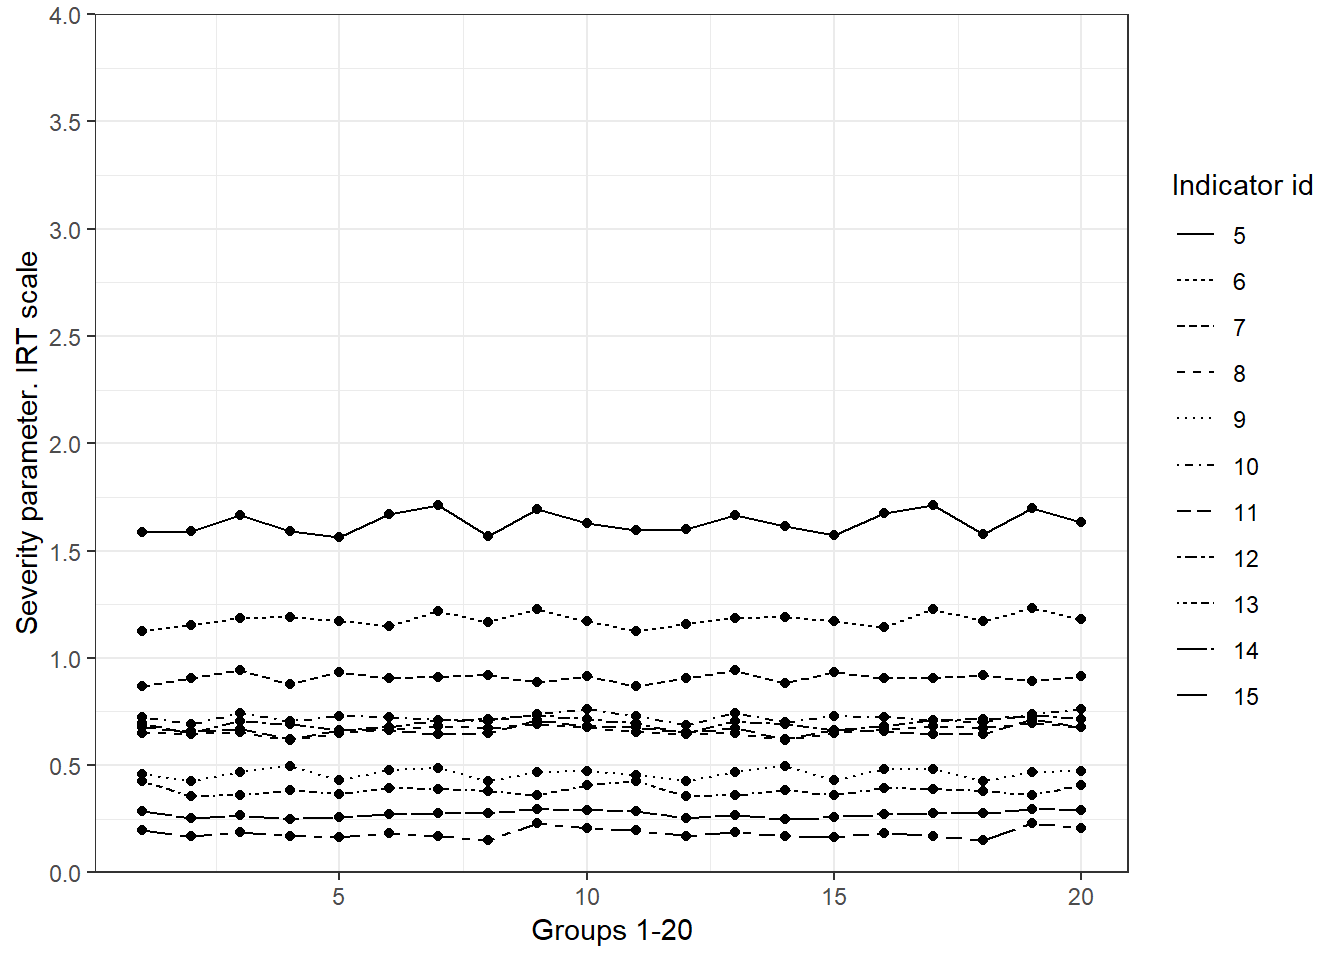
\includegraphics{PM_Book_files/figure-latex/MIhodls2-1.png}
\caption{\label{fig:MIhodls2}Severity parameters that seem to fulfil MI. Simulated data. We see very little fluctuation from one group to another}
\end{figure}

\begin{Shaded}
\begin{Highlighting}[]
\KeywordTok{ggplot}\NormalTok{(irt_MIb_nonmi,}\KeywordTok{aes}\NormalTok{(}\DataTypeTok{x=}\NormalTok{data,}\DataTypeTok{y=}\NormalTok{value,}\DataTypeTok{group=}\NormalTok{var_id)) }\OperatorTok{+}\StringTok{ }\KeywordTok{geom_point}\NormalTok{()  }\OperatorTok{+}\StringTok{ }
\StringTok{  }\KeywordTok{geom_line}\NormalTok{(}\KeywordTok{aes}\NormalTok{(}\DataTypeTok{linetype=}\KeywordTok{as.factor}\NormalTok{(var_id))) }\OperatorTok{+}\StringTok{ }
\StringTok{  }\KeywordTok{xlab}\NormalTok{(}\StringTok{"Groups 1-20"}\NormalTok{) }\OperatorTok{+}\StringTok{ }\KeywordTok{ylab}\NormalTok{(}\StringTok{"Severity parameter. IRT scale"}\NormalTok{) }\OperatorTok{+}\StringTok{ }
\StringTok{  }\KeywordTok{labs}\NormalTok{(}\DataTypeTok{linetype=}\StringTok{'Indicator id'}\NormalTok{) }\OperatorTok{+}\StringTok{  }
\StringTok{  }\KeywordTok{scale_y_continuous}\NormalTok{( }\DataTypeTok{limits =} \KeywordTok{c}\NormalTok{(}\DecValTok{0}\NormalTok{,}\DecValTok{4}\NormalTok{), }\DataTypeTok{expand =} \KeywordTok{c}\NormalTok{(}\DecValTok{0}\NormalTok{,}\DecValTok{0}\NormalTok{), }\DataTypeTok{breaks =} \KeywordTok{seq}\NormalTok{(}\DecValTok{1}\NormalTok{, }\DecValTok{4}\NormalTok{, }\FloatTok{.5}\NormalTok{) ) }\OperatorTok{+}\StringTok{ }
\StringTok{  }\KeywordTok{theme_bw}\NormalTok{()  }
\end{Highlighting}
\end{Shaded}

\begin{figure}
\centering
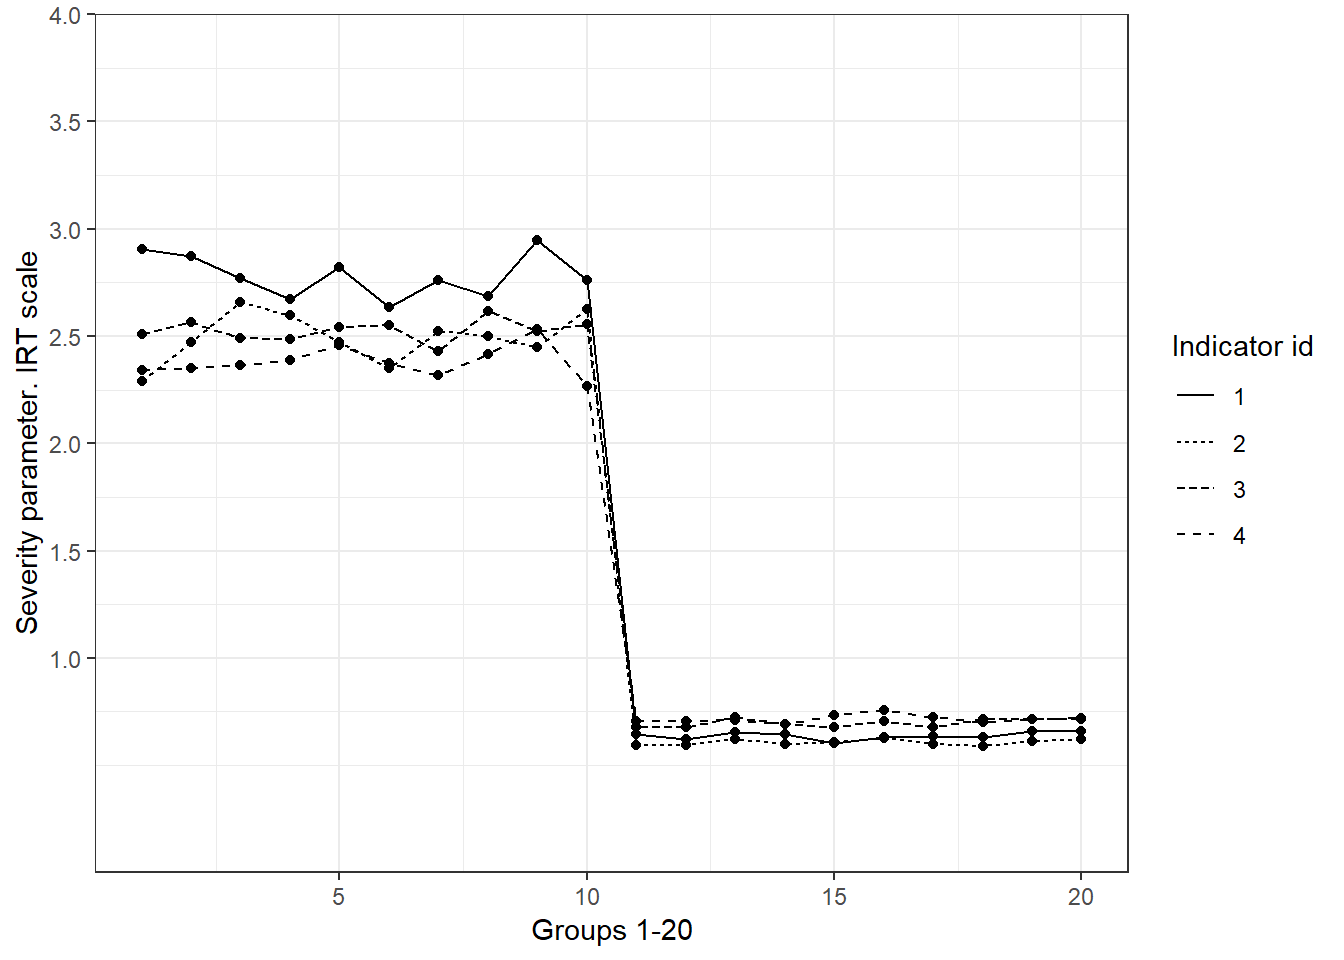
\includegraphics{PM_Book_files/figure-latex/MInothodls2-1.png}
\caption{\label{fig:MInothodls2}Severity parameters that do not seem to fulfil MI. Simulated data. We see a lot of fluctuation from groups 11-20 relative to 1-10}
\end{figure}

\hypertarget{methods-for-the-assessment-of-measurement-invariance}{%
\section{Methods for the assessment of Measurement Invariance}\label{methods-for-the-assessment-of-measurement-invariance}}

Measurement Invariance is formally examined by comparing the extent two which the parameters of a measurement model are similar between two or more groups/periods. The measurement model can be a unidimensional or a multidimensional factor model. That is, it can be seen as a formal assessment of the visual inspection shown in the previous section. The literature proposes two main methods to analyse MI: Multiple Group Factor Analysis (MGFA) and the Alignment Method (AM). The rationale behind both methods is the same, start from a measurement model with some free parameters (configural model, for example) and then move toward a model with fixed parameters (strong MI where loadings and thresholds are fixed across groups). The different models are contrasted using both absolute statistics of fit such as Chi-Square and relative statistics of fit like RMSEA and TLI, CFI. Based on these statistics researchers conclude whether the same model holds for two different groups.

\begin{Shaded}
\begin{Highlighting}[]
\NormalTok{ud_}\DecValTok{1}\NormalTok{<-}\KeywordTok{read.table}\NormalTok{(}\StringTok{"UD_data_2_1.dat"}\NormalTok{)}
\NormalTok{ud_}\DecValTok{1}\OperatorTok{$}\NormalTok{data<-}\DecValTok{2}
\NormalTok{ud_}\DecValTok{2}\NormalTok{<-}\KeywordTok{read.table}\NormalTok{(}\StringTok{"UD_data_1_1.dat"}\NormalTok{)}
\NormalTok{ud_}\DecValTok{2}\OperatorTok{$}\NormalTok{data<-}\DecValTok{1}
\NormalTok{ud_1and2<-}\KeywordTok{rbind}\NormalTok{(ud_}\DecValTok{1}\NormalTok{,ud_}\DecValTok{2}\NormalTok{)}
\KeywordTok{head}\NormalTok{(ud_1and2)}
\end{Highlighting}
\end{Shaded}

\begin{verbatim}
##   V1 V2 V3 V4 V5 V6 V7 V8 V9 V10 V11 V12 V13 V14 V15 V16 data
## 1  0  1  0  1  1  0  0  1  0   0   0   0   1   1   1   2    2
## 2  0  0  0  0  0  0  0  0  0   0   0   0   0   0   0   2    2
## 3  1  1  1  1  1  1  0  0  1   1   1   0   1   1   1   2    2
## 4  0  0  0  0  0  0  0  0  0   0   0   0   0   0   0   1    2
## 5  0  0  0  0  0  0  0  0  0   0   0   0   0   0   0   1    2
## 6  0  0  0  1  0  0  0  0  0   0   0   0   0   1   1   2    2
\end{verbatim}

\begin{Shaded}
\begin{Highlighting}[]
\KeywordTok{write.table}\NormalTok{(ud_1and2, }\DataTypeTok{file=}\StringTok{"ud_1and2.dat"}\NormalTok{, }\DataTypeTok{col.names =}\NormalTok{ F)}
\end{Highlighting}
\end{Shaded}

\hypertarget{multiple-group-factor-analysis}{%
\subsection{Multiple Group Factor Analysis}\label{multiple-group-factor-analysis}}

Multiple Group Factor Analysis had been the classic method to assess MI. To illustrate how it works on Mplus (``MI\_analysis\_du\_configural1and2.inp''), data for group 1 and group 11 (``ud\_1and2.dat'') will be used to go through the different steps involved in testing MI. The first step consist in testing the hypothesis that a configural model holds between these two groups, i.e.~whether the same unidimensional model holds leaving the loadings and thresholds free across groups. The syntax is displayed below. The syntax is very similar to the one used to fit a unidimensional Confirmatory Factor Model (CFA) following a two-parameter IRT model. One needs to tell Mplus the groups in question (GROUPING) and save the results of the Chi-square test to contrast out model with the models with fixed loadings and thresholds. It is also very important to request the Modification Indices, which tell which parameters are the sources of model miss fit and therefore the cause of violating more strict forms of MI. In this example, the mean of the latent variable is fixed to one given that those value were used to simulate these data.

\begin{Shaded}
\begin{Highlighting}[]
\NormalTok{test <-}\StringTok{ }\KeywordTok{mplusObject}\NormalTok{(}
\DataTypeTok{TITLE =} \StringTok{"Multiple Group Analysis;"}\NormalTok{,}
\DataTypeTok{VARIABLE =} \StringTok{"}
\StringTok{Name = id V1-V16 data;}
\StringTok{Missing are all (-9999) ;}
\StringTok{usevariables = V1-V15;}
\StringTok{categorical = V1-V15;}
\StringTok{GROUPING = data (1=ONE 2=TWO);"}\NormalTok{,}

\DataTypeTok{ANALYSIS=}\StringTok{"ESTIMATOR IS WLSMV; }
\StringTok{PARAMETERIZATION=THETA;"}\NormalTok{,}

\DataTypeTok{SAVEDATA=} \StringTok{"DIFFTEST=Configural.dat;"}\NormalTok{,}

\DataTypeTok{OUTPUT =} \StringTok{"STDYX MODINDICES (3.84);"}\NormalTok{,}

\DataTypeTok{MODEL =} \StringTok{" }

\StringTok{! Factor loadings all estimated         }
\StringTok{F BY V1-V15* (L1-L15); }
\StringTok{ }
\StringTok{! Item thresholds all free     }
\StringTok{[v1$1-v15$1*] (T1-T15);    }

\StringTok{! Item residual variances all fixed=1     }
\StringTok{V1-V15@1; }

\StringTok{! Factor mean=0 and variance=1 for identification }
\StringTok{[f@0]; f@1; }

\StringTok{!!! CONFIGURAL MODEL FOR ALTERNATIVE GROUP      }
\StringTok{MODEL TWO:  ! Factor loadings all estimated          }

\StringTok{F BY V1-V15*; }

\StringTok{! Item thresholds all free     }
\StringTok{[v1$1-v15$1*]; }

\StringTok{! Item residual variances all fixed=1     }
\StringTok{V1-V15@1; }

\StringTok{! Factor mean=0 and variance=1 for identification }
\StringTok{[f@0]; f@1;"}\NormalTok{)}

\NormalTok{res <-}\StringTok{ }\KeywordTok{mplusModeler}\NormalTok{(test, }\DataTypeTok{modelout =} \StringTok{"MI_analysis_du_configural1and2.inp"}\NormalTok{, }
                    \DataTypeTok{writeData =} \StringTok{"never"}\NormalTok{, }
                    \DataTypeTok{hashfilename =} \OtherTok{FALSE}\NormalTok{, }
                    \DataTypeTok{dataout=}\StringTok{"ud_1and2.dat"}\NormalTok{, }\DataTypeTok{run =}\NormalTok{ 1L)}
\end{Highlighting}
\end{Shaded}

\begin{verbatim}
## 
## Running model: MI_analysis_du_configural1and2.inp 
## System command: C:\WINDOWS\system32\cmd.exe /c cd "." && "Mplus" "MI_analysis_du_configural1and2.inp" 
## Reading model:  MI_analysis_du_configural1and2.out
\end{verbatim}

The fit of the model (``MI\_analysis\_du\_configural1and2.inp'') is shown below. The fit of the model is very good. Under the Chi-Square test the model is not rejected and the relative statistics of fit point in the same direction. However, this only a reference that allow us to inspect metric (weak) MI. Should the configural model is rejected, then comparing both poverty indices very likely lead to incorrect conclusion about both prevalence and severity of poverty.

\begin{Shaded}
\begin{Highlighting}[]
\NormalTok{fitstats<-}\KeywordTok{c}\NormalTok{(}\DataTypeTok{TLI=}\NormalTok{res}\OperatorTok{$}\NormalTok{results}\OperatorTok{$}\NormalTok{summaries}\OperatorTok{$}\NormalTok{TLI, }
            \DataTypeTok{CFI=}\NormalTok{res}\OperatorTok{$}\NormalTok{results}\OperatorTok{$}\NormalTok{summaries}\OperatorTok{$}\NormalTok{CFI, }
            \DataTypeTok{Chisq=}\NormalTok{res}\OperatorTok{$}\NormalTok{results}\OperatorTok{$}\NormalTok{summaries}\OperatorTok{$}\NormalTok{ChiSqM_PValue,}
            \DataTypeTok{RMSEA=}\NormalTok{res}\OperatorTok{$}\NormalTok{results}\OperatorTok{$}\NormalTok{summaries}\OperatorTok{$}\NormalTok{RMSEA_Estimate)}
\NormalTok{fitstats}
\end{Highlighting}
\end{Shaded}

\begin{verbatim}
##    TLI    CFI  Chisq  RMSEA 
## 1.0000 1.0000 0.0133 0.0070
\end{verbatim}

The Mplus input of the metric MI model, free threshold but fixed loadings, is displayed below (``MI\_metricanalysis\_du\_1and2.inp''). To compare the fit of the configural model against the metric model it is necessary to call for the information stored in ``DIFFTEST=Configural.dat;''. The main difference between these INPUT INSTRUCTIONS and the configural model is that the loadings of the 15 items are fixed -equal across groups-. Therefore, the model will fit such assumption to the data and see whether it holds or not.

\begin{Shaded}
\begin{Highlighting}[]
\NormalTok{test <-}\StringTok{ }\KeywordTok{mplusObject}\NormalTok{(}
\DataTypeTok{TITLE =} \StringTok{"Multiple Group Analysis (Metric);"}\NormalTok{,}
\DataTypeTok{VARIABLE =} \StringTok{"}
\StringTok{Name = id V1-V16 data;}
\StringTok{Missing are all (-9999) ;}
\StringTok{usevariables = V1-V15;}
\StringTok{categorical = V1-V15;}
\StringTok{GROUPING = data (1=ONE 2=TWO);"}\NormalTok{,}

\DataTypeTok{ANALYSIS=}\StringTok{"ESTIMATOR IS WLSMV; }
\StringTok{PARAMETERIZATION=THETA;}
\StringTok{DIFFTEST= Configural.dat;"}\NormalTok{,}

\DataTypeTok{SAVEDATA=} \StringTok{"DIFFTEST=MetricA.dat;"}\NormalTok{,}

\DataTypeTok{OUTPUT =} \StringTok{"STDYX MODINDICES (3.84);"}\NormalTok{,}

\DataTypeTok{MODEL =} \StringTok{" }

\StringTok{! Factor loadings all estimated         }
\StringTok{ F BY V1-V15* (L1-L15);}
\StringTok{       }
\StringTok{! Item thresholds all free     }
\StringTok{[v1$1-v15$1*] (T1-T15);    }

\StringTok{! Item residual variances all fixed=1     }
\StringTok{V1-V15@1; }

\StringTok{! Factor mean=0 and variance=1 for identification }
\StringTok{[f@0]; f@1; }

\StringTok{!!! CONFIGURAL MODEL FOR ALTERNATIVE GROUP      }
\StringTok{MODEL TWO:  ! Factor loadings all estimated          }

\StringTok{ F BY V1-V15* (L1-L15);}

\StringTok{! Item thresholds all free     }
\StringTok{[v1$1-v15$1*]; }

\StringTok{! Item residual variances all fixed=1     }
\StringTok{V1-V15@1; }

\StringTok{! Factor mean=0 and variance=1 for identification }
\StringTok{[f@0]; f*;"}\NormalTok{)}

\NormalTok{res <-}\StringTok{ }\KeywordTok{mplusModeler}\NormalTok{(test, }\DataTypeTok{modelout =} \StringTok{"MI_metric_analysis_du_configural1and2.inp"}\NormalTok{, }
                    \DataTypeTok{writeData =} \StringTok{"never"}\NormalTok{, }
                    \DataTypeTok{hashfilename =} \OtherTok{FALSE}\NormalTok{, }
                    \DataTypeTok{dataout=}\StringTok{"ud_1and2.dat"}\NormalTok{, }\DataTypeTok{run =}\NormalTok{ 1L)}
\end{Highlighting}
\end{Shaded}

\begin{verbatim}
## 
## Running model: MI_metric_analysis_du_configural1and2.inp 
## System command: C:\WINDOWS\system32\cmd.exe /c cd "." && "Mplus" "MI_metric_analysis_du_configural1and2.inp" 
## Reading model:  MI_metric_analysis_du_configural1and2.out
\end{verbatim}

The Chi-Square Test for Difference Testing in the output of the metric MI analysis leads to the rejection of the model (\(Chi-Square<.05\)). There is also a drop in the value of the relative statistics of fit TLI and CFI. These two suggest that although the model is relatively adequate, there is a loss after fixing the loadings across groups. This is expected given that the loadings of groups 1 and 11 are very different for some of the items.

\begin{Shaded}
\begin{Highlighting}[]
\NormalTok{fitstats<-}\KeywordTok{c}\NormalTok{(}\DataTypeTok{TLI=}\NormalTok{res}\OperatorTok{$}\NormalTok{results}\OperatorTok{$}\NormalTok{summaries}\OperatorTok{$}\NormalTok{TLI, }
            \DataTypeTok{CFI=}\NormalTok{res}\OperatorTok{$}\NormalTok{results}\OperatorTok{$}\NormalTok{summaries}\OperatorTok{$}\NormalTok{CFI, }
            \DataTypeTok{Chisq=}\NormalTok{res}\OperatorTok{$}\NormalTok{results}\OperatorTok{$}\NormalTok{summaries}\OperatorTok{$}\NormalTok{ChiSqM_PValue,}
            \DataTypeTok{RMSEA=}\NormalTok{res}\OperatorTok{$}\NormalTok{results}\OperatorTok{$}\NormalTok{summaries}\OperatorTok{$}\NormalTok{RMSEA_Estimate,}
            \DataTypeTok{ChisqDIFF=}\NormalTok{res}\OperatorTok{$}\NormalTok{results}\OperatorTok{$}\NormalTok{summaries}\OperatorTok{$}\NormalTok{ChiSqDiffTest_PValue)}
\NormalTok{fitstats}
\end{Highlighting}
\end{Shaded}

\begin{verbatim}
##       TLI       CFI     Chisq     RMSEA ChisqDIFF 
##     0.992     0.993     0.000     0.031     0.000
\end{verbatim}

The modification indices of the metric model provide information about the parameters that make the main contribution to the inadequate model fit. Figure 5.2 suggested that indicators 1-4 were very likely to be non-invariant. The modification indices confirm that indeed these items are the main sources of the discrepancy between the two groups. Without prior knowledge or a clear theory of why these four items have non-invariant loadings, the suggestion would be to let these four loadings free and re-assess metric invariance. Otherwise, the alternative would be dropping these four indicators and re-examine metric MI.

res\(results\)mod\_indices{[}1:15,{]}

To assess whether partial metric MI holds, the loadings of the four items in question (1-4) were no longer fixed between groups. The syntax is omitted but the output (``mi\_metricanalysis\_b\_du\_1and2.out'') is shown below. The Chi-Square Test for Difference Testing suggest that partial metric invariance holds. Indicating that it is feasible to proceed and conduct the examination of Strong MI (scalar MI).

\begin{Shaded}
\begin{Highlighting}[]
\NormalTok{test <-}\StringTok{ }\KeywordTok{mplusObject}\NormalTok{(}
\DataTypeTok{TITLE =} \StringTok{"Multiple Group Analysis (MetricB);"}\NormalTok{,}
\DataTypeTok{VARIABLE =} \StringTok{"}
\StringTok{Name = id V1-V16 data;}
\StringTok{Missing are all (-9999) ;}
\StringTok{usevariables = V1-V15;}
\StringTok{categorical = V1-V15;}
\StringTok{GROUPING = data (1=ONE 2=TWO);"}\NormalTok{,}

\DataTypeTok{ANALYSIS=}\StringTok{"ESTIMATOR IS WLSMV; }
\StringTok{PARAMETERIZATION=THETA;}
\StringTok{DIFFTEST= Configural.dat;"}\NormalTok{,}

\DataTypeTok{SAVEDATA=} \StringTok{"DIFFTEST=MetricB.dat;"}\NormalTok{,}

\DataTypeTok{OUTPUT =} \StringTok{"STDYX MODINDICES (3.84);"}\NormalTok{,}

\DataTypeTok{MODEL =} \StringTok{" }

\StringTok{! Factor loadings all estimated         }
\StringTok{ F BY V1-V15* (L1-L15);}
\StringTok{       }
\StringTok{! Item thresholds all free     }
\StringTok{[v1$1-v15$1*] (T1-T15);    }

\StringTok{! Item residual variances all fixed=1     }
\StringTok{V1-V15@1; }

\StringTok{! Factor mean=0 and variance=1 for identification }
\StringTok{[f@0]; f@1; }

\StringTok{!!! CONFIGURAL MODEL FOR ALTERNATIVE GROUP      }
\StringTok{MODEL TWO:        }

\StringTok{ F BY V1-V15* (L1a L2a L3a L4a L5-L15);}

\StringTok{! Item thresholds all free     }
\StringTok{[v1$1-v15$1*]; }

\StringTok{! Item residual variances all fixed=1     }
\StringTok{V1-V15@1; }

\StringTok{! Factor mean=0 and variance=1 for identification }
\StringTok{[f@0]; f*;"}\NormalTok{)}

\NormalTok{res <-}\StringTok{ }\KeywordTok{mplusModeler}\NormalTok{(test, }\DataTypeTok{modelout =} \StringTok{"MI_metricanalysis_B_du_1and2.inp"}\NormalTok{, }
                    \DataTypeTok{writeData =} \StringTok{"never"}\NormalTok{, }
                    \DataTypeTok{hashfilename =} \OtherTok{FALSE}\NormalTok{, }
                    \DataTypeTok{dataout=}\StringTok{"ud_1and2.dat"}\NormalTok{, }\DataTypeTok{run =}\NormalTok{ 1L)}
\end{Highlighting}
\end{Shaded}

\begin{verbatim}
## 
## Running model: MI_metricanalysis_B_du_1and2.inp 
## System command: C:\WINDOWS\system32\cmd.exe /c cd "." && "Mplus" "MI_metricanalysis_B_du_1and2.inp" 
## Reading model:  MI_metricanalysis_B_du_1and2.out
\end{verbatim}

\begin{Shaded}
\begin{Highlighting}[]
\NormalTok{fitstats<-}\KeywordTok{c}\NormalTok{(}\DataTypeTok{TLI=}\NormalTok{res}\OperatorTok{$}\NormalTok{results}\OperatorTok{$}\NormalTok{summaries}\OperatorTok{$}\NormalTok{TLI, }
            \DataTypeTok{CFI=}\NormalTok{res}\OperatorTok{$}\NormalTok{results}\OperatorTok{$}\NormalTok{summaries}\OperatorTok{$}\NormalTok{CFI, }
            \DataTypeTok{Chisq=}\NormalTok{res}\OperatorTok{$}\NormalTok{results}\OperatorTok{$}\NormalTok{summaries}\OperatorTok{$}\NormalTok{ChiSqM_PValue,}
            \DataTypeTok{RMSEA=}\NormalTok{res}\OperatorTok{$}\NormalTok{results}\OperatorTok{$}\NormalTok{summaries}\OperatorTok{$}\NormalTok{RMSEA_Estimate,}
            \DataTypeTok{ChisqDIFF=}\NormalTok{res}\OperatorTok{$}\NormalTok{results}\OperatorTok{$}\NormalTok{summaries}\OperatorTok{$}\NormalTok{ChiSqDiffTest_PValue)}
\NormalTok{fitstats}
\end{Highlighting}
\end{Shaded}

\begin{verbatim}
##       TLI       CFI     Chisq     RMSEA ChisqDIFF 
##    1.0000    1.0000    0.4639    0.0010    1.0000
\end{verbatim}

In order to assess scalar invariance it is necessary to hold all the thresholds (intercepts) equal across groups.

\begin{Shaded}
\begin{Highlighting}[]
\NormalTok{test <-}\StringTok{ }\KeywordTok{mplusObject}\NormalTok{(}
\DataTypeTok{TITLE =} \StringTok{"Multiple Group Analysis (Scalar);"}\NormalTok{,}
\DataTypeTok{VARIABLE =} \StringTok{"}
\StringTok{Name = id V1-V16 data;}
\StringTok{Missing are all (-9999) ;}
\StringTok{usevariables = V1-V15;}
\StringTok{categorical = V1-V15;}
\StringTok{GROUPING = data (1=ONE 2=TWO);"}\NormalTok{,}

\DataTypeTok{ANALYSIS=}\StringTok{"ESTIMATOR IS WLSMV; }
\StringTok{PARAMETERIZATION=THETA;}
\StringTok{DIFFTEST= MetricB.dat;"}\NormalTok{,}

\DataTypeTok{SAVEDATA=} \StringTok{"DIFFTEST=Scalar.dat;"}\NormalTok{,}

\DataTypeTok{OUTPUT =} \StringTok{"STDYX MODINDICES (3.84);"}\NormalTok{,}

\DataTypeTok{MODEL =} \StringTok{" }

\StringTok{! Factor loadings all estimated         }
\StringTok{ F BY V1-V15* (L1-L15);}
\StringTok{       }
\StringTok{! Item thresholds all free     }
\StringTok{[v1$1-v15$1*] (T1-T15);    }

\StringTok{! Item residual variances all fixed=1     }
\StringTok{V1-V15@1; }

\StringTok{! Factor mean=0 and variance=1 for identification }
\StringTok{[f@0]; f@1; }

\StringTok{!!! CONFIGURAL MODEL FOR ALTERNATIVE GROUP      }
\StringTok{MODEL TWO:        }

\StringTok{F BY V1-V15* (L1a L2a L3a L4a L5-L15);}

\StringTok{! Item thresholds all fixed   }

\StringTok{! Item residual variances all fixed=1     }
\StringTok{V1-V15@1; }

\StringTok{! Factor mean=0 and variance=1 for identification }
\StringTok{[f@0]; f*;"}\NormalTok{)}

\NormalTok{res <-}\StringTok{ }\KeywordTok{mplusModeler}\NormalTok{(test, }\DataTypeTok{modelout =} \StringTok{"MI_scalaranalysis_du_1and2.inp"}\NormalTok{, }
                    \DataTypeTok{writeData =} \StringTok{"never"}\NormalTok{, }
                    \DataTypeTok{hashfilename =} \OtherTok{FALSE}\NormalTok{, }
                    \DataTypeTok{dataout=}\StringTok{"ud_1and2.dat"}\NormalTok{, }\DataTypeTok{run =}\NormalTok{ 1L)}
\end{Highlighting}
\end{Shaded}

\begin{verbatim}
## 
## Running model: MI_scalaranalysis_du_1and2.inp 
## System command: C:\WINDOWS\system32\cmd.exe /c cd "." && "Mplus" "MI_scalaranalysis_du_1and2.inp" 
## Reading model:  MI_scalaranalysis_du_1and2.out
\end{verbatim}

The output below (``mi\_scalaranalysis\_du\_1and2.out'') indicates that partial scalar invariance holds. It seems that for this data, it is just necessary to let the loadings of the first four items free to achieve partial scalar invariance. This suggests that after considering differences in slope the means between groups are equivalent. This does no necessarily mean that the scale is fully invariant, the effect of the first four items could lead to incorrect conclusions when comparing poverty levels between these two groups. Next section discusses the meaning of threshold non-invariance in the context of poverty research, as this topic connects with scale equating.

\begin{Shaded}
\begin{Highlighting}[]
\NormalTok{fitstats<-}\KeywordTok{c}\NormalTok{(}\DataTypeTok{TLI=}\NormalTok{res}\OperatorTok{$}\NormalTok{results}\OperatorTok{$}\NormalTok{summaries}\OperatorTok{$}\NormalTok{TLI, }
            \DataTypeTok{CFI=}\NormalTok{res}\OperatorTok{$}\NormalTok{results}\OperatorTok{$}\NormalTok{summaries}\OperatorTok{$}\NormalTok{CFI, }
            \DataTypeTok{Chisq=}\NormalTok{res}\OperatorTok{$}\NormalTok{results}\OperatorTok{$}\NormalTok{summaries}\OperatorTok{$}\NormalTok{ChiSqM_PValue,}
            \DataTypeTok{RMSEA=}\NormalTok{res}\OperatorTok{$}\NormalTok{results}\OperatorTok{$}\NormalTok{summaries}\OperatorTok{$}\NormalTok{RMSEA_Estimate,}
            \DataTypeTok{ChisqDIFF=}\NormalTok{res}\OperatorTok{$}\NormalTok{results}\OperatorTok{$}\NormalTok{summaries}\OperatorTok{$}\NormalTok{ChiSqDiffTest_PValue)}
\NormalTok{fitstats}
\end{Highlighting}
\end{Shaded}

\begin{verbatim}
##       TLI       CFI     Chisq     RMSEA ChisqDIFF 
##     0.989     0.989     0.000     0.038     0.000
\end{verbatim}

After fixing the thresholds of the first four items partial scalar invariance holds (\(Chi-square>.05\)). This would mean that in order to meet exact scalar invariance the four items in question must be dropped from the index. This is, of course, not ideal as most of the time poverty indices have few items to choose from.

\begin{Shaded}
\begin{Highlighting}[]
\NormalTok{test <-}\StringTok{ }\KeywordTok{mplusObject}\NormalTok{(}
\DataTypeTok{TITLE =} \StringTok{"Multiple Group Analysis (ScalarB);"}\NormalTok{,}
\DataTypeTok{VARIABLE =} \StringTok{"}
\StringTok{Name = id V1-V16 data;}
\StringTok{Missing are all (-9999) ;}
\StringTok{usevariables = V1-V15;}
\StringTok{categorical = V1-V15;}
\StringTok{GROUPING = data (1=ONE 2=TWO);"}\NormalTok{,}

\DataTypeTok{ANALYSIS=}\StringTok{"ESTIMATOR IS WLSMV; }
\StringTok{PARAMETERIZATION=THETA;}
\StringTok{DIFFTEST= MetricB.dat;"}\NormalTok{,}

\DataTypeTok{SAVEDATA=} \StringTok{"DIFFTEST=ScalarB.dat;"}\NormalTok{,}

\DataTypeTok{OUTPUT =} \StringTok{"STDYX MODINDICES (3.84);"}\NormalTok{,}

\DataTypeTok{MODEL =} \StringTok{" }

\StringTok{! Factor loadings all estimated         }
\StringTok{ F BY V1-V15* (L1-L15);}
\StringTok{       }
\StringTok{! Item thresholds all free     }
\StringTok{[v1$1-v15$1*] (T1-T15);    }

\StringTok{! Item residual variances all fixed=1     }
\StringTok{V1-V15@1; }

\StringTok{! Factor mean=0 and variance=1 for identification }
\StringTok{[f@0]; f@1; }

\StringTok{!!! CONFIGURAL MODEL FOR WOMEN ALTERNATIVE GROUP      }
\StringTok{MODEL TWO:        }

\StringTok{F BY V1-V15* (L1a L2a L3a L4a L5-L15);}

\StringTok{! Item thresholds four first fixed   }
\StringTok{[v1$1-v4$1*];}

\StringTok{! Item residual variances all fixed=1     }
\StringTok{V1-V15@1; }

\StringTok{! Factor mean=0 and variance=1 for identification }
\StringTok{[f@0]; f*;"}\NormalTok{)}

\NormalTok{res <-}\StringTok{ }\KeywordTok{mplusModeler}\NormalTok{(test, }\DataTypeTok{modelout =} \StringTok{"MI_scalaranalysis_B_du_1and2.inp"}\NormalTok{, }
                    \DataTypeTok{writeData =} \StringTok{"never"}\NormalTok{, }
                    \DataTypeTok{hashfilename =} \OtherTok{FALSE}\NormalTok{, }
                    \DataTypeTok{dataout=}\StringTok{"ud_1and2.dat"}\NormalTok{, }\DataTypeTok{run =}\NormalTok{ 1L)}
\end{Highlighting}
\end{Shaded}

\begin{verbatim}
## 
## Running model: MI_scalaranalysis_B_du_1and2.inp 
## System command: C:\WINDOWS\system32\cmd.exe /c cd "." && "Mplus" "MI_scalaranalysis_B_du_1and2.inp" 
## Reading model:  MI_scalaranalysis_B_du_1and2.out
\end{verbatim}

\begin{Shaded}
\begin{Highlighting}[]
\NormalTok{fitstats<-}\KeywordTok{c}\NormalTok{(}\DataTypeTok{TLI=}\NormalTok{res}\OperatorTok{$}\NormalTok{results}\OperatorTok{$}\NormalTok{summaries}\OperatorTok{$}\NormalTok{TLI, }
            \DataTypeTok{CFI=}\NormalTok{res}\OperatorTok{$}\NormalTok{results}\OperatorTok{$}\NormalTok{summaries}\OperatorTok{$}\NormalTok{CFI, }
            \DataTypeTok{Chisq=}\NormalTok{res}\OperatorTok{$}\NormalTok{results}\OperatorTok{$}\NormalTok{summaries}\OperatorTok{$}\NormalTok{ChiSqM_PValue,}
            \DataTypeTok{RMSEA=}\NormalTok{res}\OperatorTok{$}\NormalTok{results}\OperatorTok{$}\NormalTok{summaries}\OperatorTok{$}\NormalTok{RMSEA_Estimate,}
            \DataTypeTok{ChisqDIFF=}\NormalTok{res}\OperatorTok{$}\NormalTok{results}\OperatorTok{$}\NormalTok{summaries}\OperatorTok{$}\NormalTok{ChiSqDiffTest_PValue)}
\NormalTok{fitstats}
\end{Highlighting}
\end{Shaded}

\begin{verbatim}
##       TLI       CFI     Chisq     RMSEA ChisqDIFF 
##    1.0000    1.0000    0.7059    0.0000    0.9611
\end{verbatim}

\hypertarget{the-alignment-method}{%
\subsection{The alignment method}\label{the-alignment-method}}

Multiple Group Factor Analysis has some disadvantages in real-data settings. In a real-data situation, researchers will have to fit a number of models to have an idea of the different sources of non-invariance. This is time-consuming and compromises the reproducibility of the findings given that another researcher might use different criteria to go through the modification indices. Another problem is that the MGFA is not feasible for many groups. Another disadvantage, when using Chi-Square, is that the models will be almost always rejected with large samples and researchers, therefore, have to work with rules of thumb to assess sufficient changes in TLI or CFI.

The alignment method has been put forward to overcome some of the drawbacks of MGFA. In particular, it simplifies the assessment of MI when having many groups. This method is under constant development but it aims to estimate means and variances of the latent factor conditional on a minimum level of MI. That means that it does not requires exact MI and aims at approximately MI. The alignment method therefore seeks an optional degree of measurement invariance given the data. The alignment method starts from the assumption that the configural model will be better that the fully scalar model. Once a configural model is fitted (M0), then the alignment method looks for a model that is equally as good as M0 but with some fixed parameters. By minimizing the loss function due to non-invariant parameters, the alignment method estimates factor means that are comparable conditional on the approximately invariant model.

\begin{Shaded}
\begin{Highlighting}[]
\NormalTok{temp =}\StringTok{ }\KeywordTok{list.files}\NormalTok{(}\DataTypeTok{pattern=}\StringTok{"UD_data_.*.dat"}\NormalTok{)}
\NormalTok{myfiles =}\StringTok{ }\KeywordTok{lapply}\NormalTok{(temp, read.table)}
\NormalTok{myfiles<-myfiles[}\OperatorTok{-}\DecValTok{11}\NormalTok{]}
\NormalTok{myfiles<-myfiles[}\OperatorTok{-}\DecValTok{21}\NormalTok{]}
\NormalTok{data<-}\KeywordTok{do.call}\NormalTok{(rbind,myfiles)}
\NormalTok{data}\OperatorTok{$}\NormalTok{data<-}\KeywordTok{rep}\NormalTok{(}\DecValTok{1}\OperatorTok{:}\DecValTok{20}\NormalTok{,}\DataTypeTok{each=}\DecValTok{5000}\NormalTok{)}
\KeywordTok{write.table}\NormalTok{(data,}\DataTypeTok{file=}\StringTok{"UD_MI_AM.dat"}\NormalTok{, }\DataTypeTok{col.names =}\NormalTok{ F)}
\end{Highlighting}
\end{Shaded}

To introduce the key aspects of the alignment method, this section relies on the simulated data generated for the 20 groups. A data set was created containing the 15 indicators for each case in the sample (\(n=5000\)) for each group (``UD\_MI\_AM.dat''). The alignment method is easily implemented on Mplus using the INPUT INSTRUCTIONS below (``UD\_MI\_AM.inp''). Mplus requires the name of the variable containing the group ids as well as the total number of groups (classes). Then a unidimensional factor model is specified. Mplus produces some useful plots to visualise, in this case, the IRT parameters of the model. This is similar to Figures 5.1 to 5.4.

\begin{verbatim}
INPUT INSTRUCTIONS

  Data:
    File is UD_MI_AM.dat ;
  Variable:
    Names are id V1-V16 data;
    Missing are all (-9999) ;

  usevariables = V1-V15;

  categorical = V1-V15;

  classes = c(20);
  knownclass = c(data = 1 2 3 4 5 6 7 8 9 10
                         11 12 13 14 15 16 17 18 19 20);


  Analysis:  type = mixture;
            estimator = ml;
            alignment = free;
            ALGORITHM=INTEGRATION;
            Process=8;

  model:
            %overall%
            f by V1-V15;


    output:
            tech1 tech8 align;

    plot:
            type = plot2;
\end{verbatim}

The results of the alignment method are displayed below. In rows the output indicates whether the parameter is variant or non-invariant (in brackets). The number corresponds to the number of the group. These findings suggest that all the thresholds are invariant and that all the loadings of items 5 to 15 (V5 to V20) are invariant. The loadings of the first four items are non-invariant. These results are consistent with the findings of the MGFA. However, in this case the analysis is performed for the 20 groups and only one model needed to be fitted to the data. The alignment method indicates that for these data is possible to minimize non-invariance if the loadings of items 1 to 4 (V1 to V4) are not fixed for groups 11 to 20. Therefore, the results suggest that partial scalar invariance holds for this simulated example.

The alignment method suggest that the 20 poverty indices are comparable once the non-invariance of the loadings of the first four items is accounted by for.

\begin{verbatim}
APPROXIMATE MEASUREMENT INVARIANCE (NONINVARIANCE) FOR GROUPS

 Intercepts/Thresholds
   V1$1        1 2 3 4 5 6 7 8 9 10 11 12 13 14 15 16 17 18 19 20
   V2$1        1 2 3 4 5 6 7 8 9 10 11 12 13 14 15 16 17 18 19 20
   V3$1        1 2 3 4 5 6 7 8 9 10 11 12 13 14 15 16 17 18 19 20
   V4$1        1 2 3 4 5 6 7 8 9 10 11 12 13 14 15 16 17 18 19 20
   V5$1        1 2 3 4 5 6 7 8 9 10 11 12 13 14 15 16 17 18 19 20
   V6$1        1 2 3 4 5 6 7 8 9 10 11 12 13 14 15 16 17 18 19 20
   V7$1        1 2 3 4 5 6 7 8 9 10 11 12 13 14 15 16 17 18 19 20
   V8$1        1 2 3 4 5 6 7 8 9 10 11 12 13 14 15 16 17 18 19 20
   V9$1        1 2 3 4 5 6 7 8 9 10 11 12 13 14 15 16 17 18 19 20
   V10$1       1 2 3 4 5 6 7 8 9 10 11 12 13 14 15 16 17 18 19 20
   V11$1       1 2 3 4 5 6 7 8 9 10 11 12 13 14 15 16 17 18 19 20
   V12$1       1 2 3 4 5 6 7 8 9 10 11 12 13 14 15 16 17 18 19 20
   V13$1       1 2 3 4 5 6 7 8 9 10 11 12 13 14 15 16 17 18 19 20
   V14$1       1 2 3 4 5 6 7 8 9 10 11 12 13 14 15 16 17 18 19 20
   V15$1       1 2 3 4 5 6 7 8 9 10 11 12 13 14 15 16 17 18 19 20

 Loadings for F
   V1          1 2 3 4 5 6 7 8 9 10 (11) (12) (13) (14) (15) (16) (17) (18) (19) (20)
   V2          1 2 3 4 5 6 7 8 9 10 (11) (12) (13) (14) (15) (16) (17) (18) (19) (20)
   V3          1 2 3 4 5 6 7 8 9 10 (11) (12) (13) (14) (15) (16) (17) (18) (19) (20)
   V4          1 2 3 4 5 6 7 8 9 10 (11) (12) (13) (14) (15) (16) (17) (18) (19) (20)
   V5          1 2 3 4 5 6 7 8 9 10 11 12 13 14 15 16 17 18 19 20
   V6          1 2 3 4 5 6 7 8 9 10 11 12 13 14 15 16 17 18 19 20
   V7          1 2 3 4 5 6 7 8 9 10 11 12 13 14 15 16 17 18 19 20
   V8          1 2 3 4 5 6 7 8 9 10 11 12 13 14 15 16 17 18 19 20
   V9          1 2 3 4 5 6 7 8 9 10 11 12 13 14 15 16 17 18 19 20
   V10         1 2 3 4 5 6 7 8 9 10 11 12 13 14 15 16 17 18 19 20
   V11         1 2 3 4 5 6 7 8 9 10 11 12 13 14 15 16 17 18 19 20
   V12         1 2 3 4 5 6 7 8 9 10 11 12 13 14 15 16 17 18 19 20
   V13         1 2 3 4 5 6 7 8 9 10 11 12 13 14 15 16 17 18 19 20
   V14         1 2 3 4 5 6 7 8 9 10 11 12 13 14 15 16 17 18 19 20
   V15         1 2 3 4 5 6 7 8 9 10 11 12 13 14 15 16 17 18 19 20
\end{verbatim}

\hypertarget{real-data-analysis-of-measurement-invariance}{%
\section{Real-data analysis of Measurement Invariance}\label{real-data-analysis-of-measurement-invariance}}

Strong (or Scalar) measurement invariance is unlikely to hold when working with real data. The analysis of MI is fairly new in poverty research that there is no agreement about what the desirable level of MI should be.@Guio2017 found partial scalar MI using the EU-SILC data and Najera (\protect\hyperlink{ref-Najera2016}{2016}) found partial scalar MI for the official Mexican multidimensional measure. Both exercises conclude that the ideal is scalar MI but that in practice partial scalar is a more sensible standard. Both non-invariant thresholds and loadings are likely to appear in real-data analyses but given that differences in difficulty -thresholds- could be more explicitly accounted by for in scale equating -next chapter- one sensible recommendation is to maximize metric invariance and then move onto partial scalar invariance.

The INPUT INSTRUCTIONS of the MI analysis of the FRS data (``FRS\_mplusprep.dat'') are shown below. The data set contains all the 25 deprivation indicators, sampling weights (gross4) and the household id (id). There is data available for ten periods (2004/2005 to 2013/2104). However, four variables were replaced by another four in 2011. Therefore, the MI analysis is performed using the 17 common variables across both periods -next chapter concerns with the issue of equating and scaling measures with different and non-invariant indicators). The classes in the INPUT INSTRUCTIONS are the 10 years (ordered were 1=2004/2005, \ldots, 10=2013-2014). For the purposes of the illustration cluster sampling is assumed but we recommend checking the Mplus manual for deeper understanding of working with complex samples.

\begin{verbatim}
INPUT INSTRUCTIONS

  Data:
    File is FRS_mplusprep.dat ;
  Variable:
    Names are
       gross4 FRSYear dep_ADDDEC dep_ADDEPLES dep_ADDHOL 
       dep_ADDINS dep_ADDMEL dep_ADDMON dep_ADDSHOE dep_ADEPFUR 
       dep_AF1 dep_AFDEP2 dep_HOUSHE1 dep_CDELPLY dep_CDEPBED 
       dep_CDEPCEL dep_CDEPEQP dep_CDEPHOL dep_CDEPLES
       dep_CDEPSUM dep_CDEPTEA dep_CDEPTRP dep_CPLAY 
       dep_CDEPACT dep_CDEPVEG dep_CDPCOAT dep_ADBTBL id;
    Missing are all (-9999) ;

  usevariables = dep_ADDDEC  dep_ADDHOL dep_ADDINS
        dep_ADDMON  dep_ADEPFUR dep_AF1 dep_AFDEP2 dep_HOUSHE1
       dep_CDELPLY dep_CDEPBED dep_CDEPCEL dep_CDEPEQP dep_CDEPHOL 
       dep_CDEPLES dep_CDEPTEA dep_CDEPTRP dep_CPLAY;

  categorical = dep_ADDDEC  dep_ADDHOL dep_ADDINS
        dep_ADDMON  dep_ADEPFUR dep_AF1 dep_AFDEP2 dep_HOUSHE1
       dep_CDELPLY dep_CDEPBED dep_CDEPCEL dep_CDEPEQP dep_CDEPHOL 
       dep_CDEPLES dep_CDEPTEA dep_CDEPTRP dep_CPLAY;

  classes = c(10);
  knownclass = c(FRSYear = 1 2 3 4 5 6 7 8 9 10);

  weight=gross4;

  cluster=id;

  Analysis:  type = mixture complex;
            estimator = ml;
            alignment = fixed;
            ALGORITHM=INTEGRATION;
            Process=8;

  model:
            
            f by dep_ADDDEC  dep_ADDHOL dep_ADDINS
        dep_ADDMON  dep_ADEPFUR dep_AF1 dep_AFDEP2 dep_HOUSHE1
       dep_CDELPLY dep_CDEPBED dep_CDEPCEL dep_CDEPEQP 
       dep_CDEPHOL dep_CDEPLES
       dep_CDEPTEA dep_CDEPTRP dep_CPLAY;


    output:
            tech1 tech8 align;

    plot:
            type = plot2;
\end{verbatim}

One of the key outputs of the alignment method is displayed below and it shows which parameters are non-invariant (within brackets) for each year. For example, the intercept of DEP\_ADDD non-invariant for group 1 and the intercepts of DEP\_ADDH and DEP\_ADDI are invariant. The results suggest that partial scalar MI holds. This can be achieved by using a subset of items with both invariant intercepts and loadings: DEP\_ADDI, DEP\_ADEP, DEP\_AF1, DEP\_AFDE, DEP\_CDEPEQP, DEP\_CDEPHOL, DEP\_CDEPTRP and DEP\_CPLA. There are other items that are almost fully invariant as they only violate MI in one group. At this point is worth noting that the alignment method finds the parameters that maximize approximate MI and, therefore, MGFA could be used to find more items that fulfill MI once other parameters have been fixed, this the advantage but also the disadvantage of the MGFA in that it allows the researcher to find that partial scalar MI models -if exists- that suits better the purposes of her research.

\begin{verbatim}
APPROXIMATE MEASUREMENT INVARIANCE (NONINVARIANCE) FOR GROUPS

 Intercepts/Thresholds
   DEP_ADDD$1  (1) 2 3 4 5 6 7 8 9 10
   DEP_ADDH$1  1 2 3 4 5 6 7 8 9 10
   DEP_ADDI$1  1 2 3 4 5 6 7 8 9 10
   DEP_ADDM$1  (1) (2) (3) (4) 5 6 7 8 9 (10)
   DEP_ADEP$1  1 2 3 4 5 6 7 8 9 10
   DEP_AF1$1   1 2 3 4 5 6 7 8 9 10
   DEP_AFDE$1  1 2 3 4 5 6 7 8 9 10
   DEP_HOUS$1  (1) (2) 3 4 5 6 7 8 9 10
   DEP_CDEL$1  (1) (2) (3) (4) (5) 6 7 8 9 10
   DEP_CDEP$1  1 2 3 4 5 6 7 8 9 10
   DEP_CDEP$1  1 2 3 4 5 6 7 8 9 10
   DEP_CDEP$1  1 2 3 4 5 6 7 8 (9) 10
   DEP_CDEP$1  (1) 2 3 4 5 6 7 8 9 10
   DEP_CDEP$1  1 2 3 4 5 6 7 8 9 (10)
   DEP_CDEP$1  1 2 3 4 5 6 7 8 9 10
   DEP_CDEP$1  1 2 3 4 5 6 7 8 9 10
   DEP_CPLA$1  1 2 3 4 5 6 7 8 9 10

 Loadings for F
   DEP_ADDD    (1) 2 3 4 5 6 7 8 9 10
   DEP_ADDH    (1) (2) (3) (4) 5 6 7 8 9 10
   DEP_ADDI    1 2 3 4 5 6 7 8 9 10
   DEP_ADDM    1 2 3 4 5 (6) 7 8 9 (10)
   DEP_ADEP    1 2 3 4 5 6 7 8 9 10
   DEP_AF1     1 2 3 4 5 6 7 8 9 10
   DEP_AFDE    1 2 3 4 5 6 7 8 9 10
   DEP_HOUS    1 2 (3) (4) 5 6 7 8 9 10
   DEP_CDEL    1 2 3 4 5 6 7 8 9 10
   DEP_CDEP    1 2 3 4 5 6 7 8 9 10
   DEP_CDEP    1 2 3 4 5 6 7 8 9 10
   DEP_CDEP    1 2 3 4 5 6 7 8 (9) 10
   DEP_CDEP    1 2 3 4 5 6 7 8 9 10
   DEP_CDEP    (1) 2 3 4 5 6 7 8 9 10
   DEP_CDEP    1 2 3 4 5 6 7 (8) (9) 10
   DEP_CDEP    1 2 3 4 5 6 7 8 9 10
   DEP_CPLA    1 2 3 4 5 6 7 8 9 10
\end{verbatim}

One of the key purposes of the alignment method is to compare groups on the factor mean once approximate MI is met. The results suggest that the severity of child deprivation has remained pretty much the same. Years, 5 (2008/09), 6 (2009/10) and 7 (2010/11), however, have significantly smaller means compared with 2004/2005. This suggest that in the observed period and with these 17 indicators, child deprivation was at its lowest level in 2008/09 (pre-economic crisis). It seems that after the year 2010/11 severity increased and reached similar levels of the early 2000s.

\begin{verbatim}
FACTOR MEAN COMPARISON AT THE 5% SIGNIFICANCE LEVEL IN DESCENDING ORDER

 Results for Factor F

           Latent    Group      Factor
 Ranking    Class    Value       Mean     Groups With Significantly
                                          Smaller Factor Mean
     1         1         1       0.000    6 7 5
     2         4         4      -0.005    5
     3         3         3      -0.011    5
     4         9         9      -0.014    5
     5        10        10      -0.029
     6         8         8      -0.034
     7         2         2      -0.036
     8         6         6      -0.042
     9         7         7      -0.048
    10         5         5      -0.065
\end{verbatim}

\begin{Shaded}
\begin{Highlighting}[]
\KeywordTok{library}\NormalTok{(haven)}
\KeywordTok{library}\NormalTok{(plyr)}

\NormalTok{D<-}\KeywordTok{read_dta}\NormalTok{(}\StringTok{"FRS_mplusprep.dta"}\NormalTok{)}

\ControlFlowTok{if}\NormalTok{(D}\OperatorTok{$}\NormalTok{FRSYear}\OperatorTok{<=}\DecValTok{7}\NormalTok{) \{}
\NormalTok{  D}\OperatorTok{$}\NormalTok{ds_uw<-}\KeywordTok{rowSums}\NormalTok{(D[,}\KeywordTok{c}\NormalTok{(}\DecValTok{3}\OperatorTok{:}\DecValTok{23}\NormalTok{)],}\DataTypeTok{na.rm=}\OtherTok{TRUE}\NormalTok{)}
\NormalTok{\} }\ControlFlowTok{else}\NormalTok{ \{}
  \KeywordTok{rowSums}\NormalTok{(D[,}\KeywordTok{c}\NormalTok{(}\DecValTok{3}\NormalTok{,}\DecValTok{5}\NormalTok{,}\DecValTok{6}\NormalTok{,}\DecValTok{8}\NormalTok{,}\DecValTok{10}\NormalTok{,}\DecValTok{11}\OperatorTok{:}\DecValTok{19}\NormalTok{,}\DecValTok{21}\OperatorTok{:}\DecValTok{27}\NormalTok{)],}\DataTypeTok{na.rm=}\OtherTok{TRUE}\NormalTok{)}
\NormalTok{\}}

\NormalTok{ds_frs<-}\KeywordTok{ddply}\NormalTok{(D,.(FRSYear), summarise, }\DataTypeTok{mean_ds=}\KeywordTok{mean}\NormalTok{(ds_uw))}
\NormalTok{ds_frs}\OperatorTok{$}\NormalTok{year<-}\KeywordTok{c}\NormalTok{(}\StringTok{"2004/2005"}\NormalTok{,}\StringTok{"2005/2006"}\NormalTok{,}\StringTok{"2006/2007"}\NormalTok{,}\StringTok{"2007/2008"}\NormalTok{,}\StringTok{"2008/2009"}\NormalTok{,}\StringTok{"2009/2010"}\NormalTok{,}\StringTok{"2010/2011"}\NormalTok{,}\StringTok{"2011/2012"}\NormalTok{,}
                   \StringTok{"2012/2013"}\NormalTok{,}\StringTok{"2013/2014"}\NormalTok{)}
\NormalTok{frs_raw<-}\KeywordTok{data.frame}\NormalTok{(}\DataTypeTok{ds_raw=}\KeywordTok{c}\NormalTok{(}\FloatTok{0.000}\NormalTok{ , }\FloatTok{-0.005}\NormalTok{,  }\FloatTok{-0.011}\NormalTok{, }\FloatTok{-0.014}\NormalTok{, }\FloatTok{-0.029}\NormalTok{, }\FloatTok{-0.034}\NormalTok{, }\FloatTok{-0.036}\NormalTok{, }\FloatTok{-0.042}\NormalTok{, }\FloatTok{-0.048}\NormalTok{, }\FloatTok{-0.065}\NormalTok{), }\DataTypeTok{FRSYear=}\KeywordTok{c}\NormalTok{(}\DecValTok{1}\NormalTok{,}\DecValTok{4}\NormalTok{,}\DecValTok{3}\NormalTok{,}\DecValTok{9}\NormalTok{,}\DecValTok{10}\NormalTok{,}\DecValTok{8}\NormalTok{,}\DecValTok{2}\NormalTok{,}\DecValTok{6}\NormalTok{,}\DecValTok{7}\NormalTok{,}\DecValTok{5}\NormalTok{))}
\NormalTok{ds_frs<-}\KeywordTok{merge}\NormalTok{(ds_frs,frs_raw,}\DataTypeTok{by=}\StringTok{"FRSYear"}\NormalTok{)}
\end{Highlighting}
\end{Shaded}

Figure \ref{fig:MIFRScomp} plots the raw child deprivation score (0-17 count) and the adjusted factor score. When a scale is highly reliable and fully invariant, the raw mean and the factor score must be highly (negatively) correlated. The plot does not shows a clear correlation. The MI analysis suggested that several parameters need to be taken into account for the scale to be comparable over time. Whereas the raw deprivation score suggest that severity of deprivation has decreased over time (particularly after 2011), the MI analysis suggest that this is not the case as the scale lost comparability. Therefore, researchers relying on raw scores or any other transformation that does not takes into account non-invariance are likely to arrive to incorrect conclusions about the trends in child deprivation.

\begin{figure}[H]

{\centering 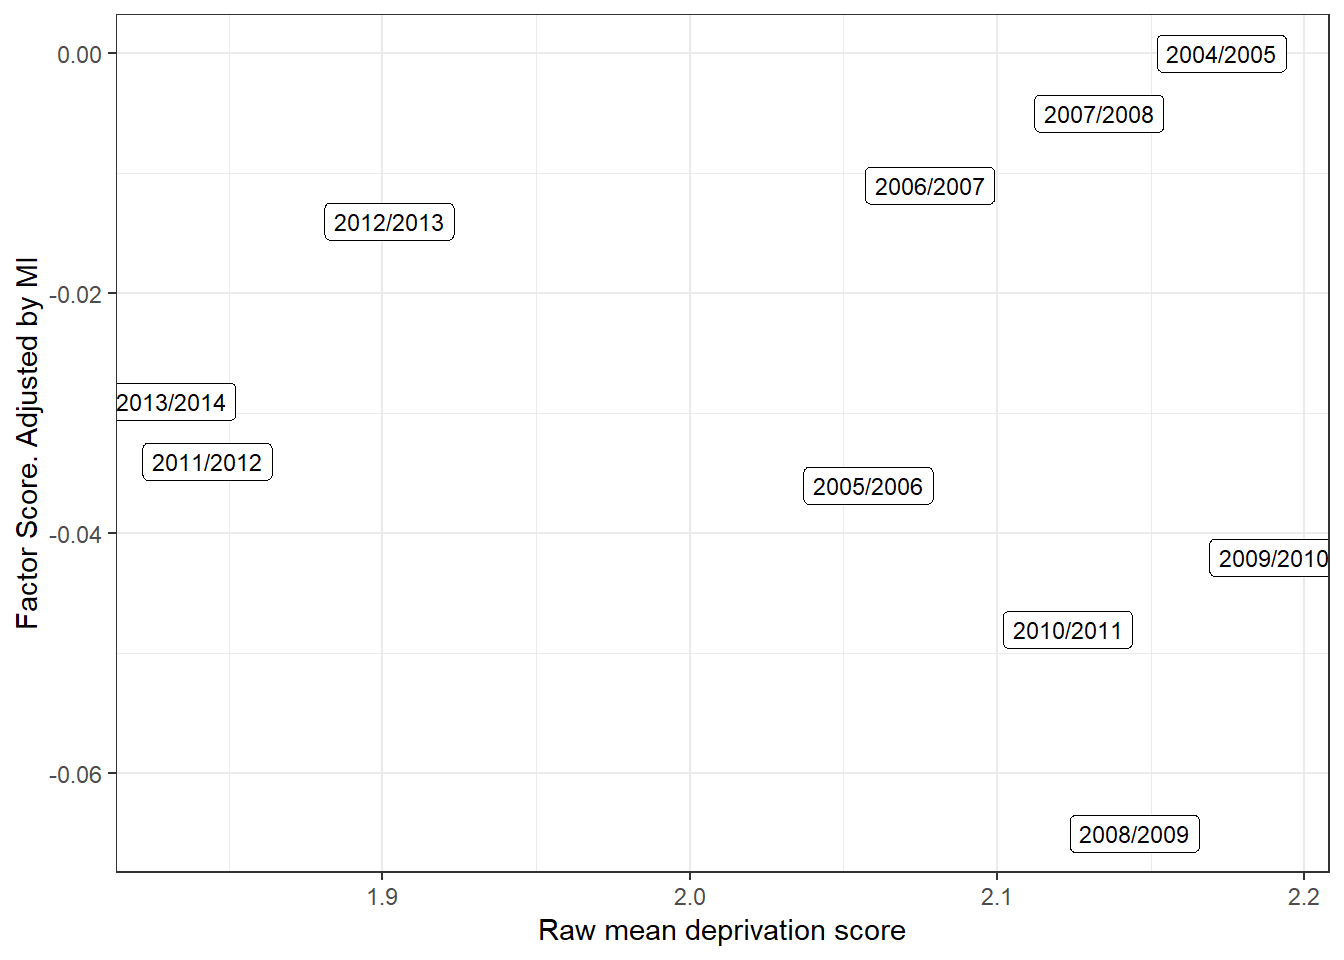
\includegraphics{PM_Book_files/figure-latex/MIFRScomp-1} 

}

\caption{Scatter plot with a comparison of the raw mean child deprivation score (simple count) and the factor adjusted score. FRS data 2004-2013. The plot shows that there a great deal of discrepancy between the adjusted and the unadjusted severity scores. Conclusions about the depth of poverty are affected by the comparability of the data over time.}\label{fig:MIFRScomp}
\end{figure}

Prevalence weighting has been a means to consider the severity of item-level deprivation in the estimation of overall deprivation and poverty ({\textbf{???}}). This procedure consists in assigning more weight to those items that most people have in the society in question. As discussed in the chapter on Reliability, an index is self-weighting for high reliability values. Therefore, very little is gained when using differential weighting. However, when comparing groups or years weighting could help to improve the comparability of a measure as this procedure is directly associated with the difficulty/severity parameter. Adjusting by differences in severity is one way to improve comparisons across groups. The next chapter, therefore, focuses on how equating, linking and scaling can be used to make scales comparable.

\hypertarget{scale-equating-and-linking}{%
\chapter{Scale equating and linking}\label{scale-equating-and-linking}}

\hypertarget{intuition-to-scale-equation}{%
\section{Intuition to scale equation}\label{intuition-to-scale-equation}}

Previous chapter introduces the sources affecting the comparability of different poverty indices and presents the concept and empirical implementation of measurement invariance. In poverty research, households are ranked according to some indicators of (low) living standards using survey or census data. The indicators in question have a structure (unidimensional or multidimensional, See chapter X) for the population in question. One problem is that such a measurement model might not be adequate for a different population or for a different year. That is, the measurement model is not equivalent (see previous chapter). Therefore, we would like to assess whether a measure is equivalent across populations/periods. Once this assessment is conducted poverty can be compared on the factor using the aligment method. This, however, might not be fully satisfactory for policy makers as the values of a standarized latent variable make little practical sense. Furthermore, it is unclear how to use these values to set a poverty line.

Another critical problem is that MI is adequate when scales have the same items and it does not solve the problem of working with scales that have different items or that have been upgraded in accordance with the living standards. Ideally, once measurement invariance is assessed researches would like to put everything into a meaninful metric and being able to compare measures that might have suffered from changes in its contents. Moreover, one question in poverty research is about how the severity of poverty is affected by changes in living standards and how this can be tractable using the available data.

\hypertarget{theory-of-scale-equating}{%
\section{Theory of scale equating}\label{theory-of-scale-equating}}

\hypertarget{example-with-simulated-data-in-r}{%
\section{Example with simulated data in R}\label{example-with-simulated-data-in-r}}

\hypertarget{real-data-example-2}{%
\section{Real-data example}\label{real-data-example-2}}

\hypertarget{identifying-the-poor-group}{%
\chapter{Identifying the poor group}\label{identifying-the-poor-group}}

\hypertarget{the-poverty-line}{%
\section{The poverty line}\label{the-poverty-line}}

\hypertarget{perspectives-on-the-poverty-line-union-and-intersection-approaches}{%
\section{Perspectives on the poverty line: Union and intersection approaches}\label{perspectives-on-the-poverty-line-union-and-intersection-approaches}}

\hypertarget{the-human-rights-based-approach}{%
\section{The human rights-based approach}\label{the-human-rights-based-approach}}

\hypertarget{the-ubn-weighted-approach}{%
\section{The UBN weighted approach}\label{the-ubn-weighted-approach}}

\hypertarget{the-partially-weighted-approach}{%
\section{The partially-weighted approach}\label{the-partially-weighted-approach}}

\hypertarget{the-bristol-optimal-approach}{%
\section{The Bristol Optimal approach}\label{the-bristol-optimal-approach}}

\hypertarget{example-with-simulated-data}{%
\section{Example with simulated data}\label{example-with-simulated-data}}

\hypertarget{real-data-analysis}{%
\section{Real-data analysis}\label{real-data-analysis}}

\hypertarget{final-thoughts}{%
\chapter{Final thoughts}\label{final-thoughts}}

\hypertarget{the-future-of-data-production-in-multidimensional-poverty-measurement}{%
\section{The future of data production in multidimensional poverty measurement}\label{the-future-of-data-production-in-multidimensional-poverty-measurement}}

\hypertarget{advanced-topics-in-multidimensional-poverty-measurement}{%
\section{Advanced topics in multidimensional poverty measurement}\label{advanced-topics-in-multidimensional-poverty-measurement}}

\hypertarget{references}{%
\chapter{References}\label{references}}

\hypertarget{refs}{}
\leavevmode\hypertarget{ref-AERA2014}{}%
AERA, APA and NCME. (2014). Standards for educational and psychological testing. (American Educational Research (AERA) and American Psychological Association (APA) and National Council on Measurement in Education (NCME) and Joint Committee on Standards for Educational and Psychological Testing (US), Ed.). Amer Educational Research Assn.

\leavevmode\hypertarget{ref-Alkire2007}{}%
Alkire, S. (2007). Choosing dimensions: The capability approach and multidimensional poverty. In \emph{The many dimensions of poverty} (pp. 89--119). Springer.

\leavevmode\hypertarget{ref-Alkire2011a}{}%
Alkire, S., \& Foster, J. (2011). Counting and multidimensional poverty measurement. \emph{Journal of Public Economics}, \emph{95}(7), 476--487.

\leavevmode\hypertarget{ref-Alkire2011}{}%
Alkire, S., \& Roche, J. (2011). \emph{Beyond headcount: Measures that reflect the breath and components of child poverty} (No. 2). Oxford Poverty; Human Development Initiative (OPHI).

\leavevmode\hypertarget{ref-Alkire2015}{}%
Alkire, S., Roche, J. M., Ballon, P., Foster, J., Santos, M. E., \& Seth, S. (2015). \emph{Multidimensional poverty measurement and analysis}. Oxford University Press, USA.

\leavevmode\hypertarget{ref-Alkire2010}{}%
Alkire, S., \& Santos, M. (2010). \emph{Acute multidimensional poverty: A new index for developing countries}. OPHI Working Paper No. 38.

\leavevmode\hypertarget{ref-Allen2001}{}%
Allen, M. J., \& Yen, W. M. (2001). \emph{Introduction to measurement theory}. Waveland Press.

\leavevmode\hypertarget{ref-Altimir1979}{}%
Altimir, O. (1979). \emph{La dimensión de la pobreza en América Latina}. CEPAL.

\leavevmode\hypertarget{ref-Atkinson2017}{}%
Atkinson, A. B., Guio, A.-C., \& Marlier, E. (2017). \emph{Monitoring social inclusion in europe}. Publications Office of the European Union.

\leavevmode\hypertarget{ref-Bandalos2018}{}%
Bandalos, D. L. (2018). \emph{Measurement theory and applications for the social sciences}. Guilford Publications.

\leavevmode\hypertarget{ref-Bartholomew1987}{}%
Bartholomew, D. J. (1987). \emph{Latent variables models and factor analysis.} (D. J. Bartholomew, Ed.). New York: Oxford University Press.

\leavevmode\hypertarget{ref-Bentler2007}{}%
Bentler, P. M. (2007). On tests and indices for evaluating structural models. \emph{Personality and Individual Differences}, \emph{42}(5), 825--829. doi:\href{https://doi.org/http://dx.doi.org/10.1016/j.paid.2006.09.024}{http://dx.doi.org/10.1016/j.paid.2006.09.024}

\leavevmode\hypertarget{ref-Betti2015}{}%
Betti, G., Gagliardi, F., Lemmi, A., \& Verma, V. (2015). Comparative measures of multidimensional deprivation in the european union. \emph{Empirical Economics}, \emph{49}(3), 1071--1100.

\leavevmode\hypertarget{ref-Bock1981}{}%
Bock, R. D., \& Aitkin, M. (1981). Marginal maximum likelihood estimation of item parameters: Application of an em algorithm. \emph{Psychometrika}, \emph{46}(4), 443--459. doi:\href{https://doi.org/10.1007/BF02293801}{10.1007/BF02293801}

\leavevmode\hypertarget{ref-Boltvinik1992}{}%
Boltvinik, J. (1992). El método de medición integrada de la pobreza. Una propuesta para su desarrollo. \emph{Comercio Exterior}, \emph{42}(4), 354--365.

\leavevmode\hypertarget{ref-Boltvinik1998}{}%
Boltvinik, J. (1998). \emph{Poverty measurement methods: An overview}. Series on Poverty Reduction: An overview.

\leavevmode\hypertarget{ref-Boltvinik2014}{}%
Boltvinik, J. (2014). América Latina, de la vanguardia al rezago en medición multidimensional de la pobreza. La experiencia contrastante de México . Una guía para la región. In J. et a. Boltviniki (Ed.), \emph{La multidimensionalidad como un desafío para los métdos y técnicas de la medición de la pobreza}. CLACSO-CROP.

\leavevmode\hypertarget{ref-Boltvinik2001}{}%
Boltvinik, J., \& Hernández-Láos, H. (2001). \emph{Pobreza y distribución del ingreso en México}. (J. Boltvinik \& H. Hernández-Láos, Eds.). Siglo XXI Editores.

\leavevmode\hypertarget{ref-Bradshaw1993}{}%
Bradshaw, J. (1993). \emph{Budget standards for the united kingdom.} (J. Bradshaw, Ed.). Aldershot: Avebury.

\leavevmode\hypertarget{ref-Bradshaw1995}{}%
Bradshaw, J., Holmes, H., \& Hallerod, B. (1995). Adapting the consensual definition of poverty. \emph{Breadline Britain in the 1990s, Department of Social Policy and Planning, University of Bristol, Bristol}.

\leavevmode\hypertarget{ref-Bradshaw2008}{}%
Bradshaw, J., Middleton, S., Davis, A., Oldfeld, N., Smith, N., Cusworth, L., \& Williams, J. (2008). \emph{A minimum income standard for britain}. Creative Commons. Retrieved from \url{https://dspace.lboro.ac.uk/dspace-jspui/bitstream/2134/3465/1/2226-income-poverty-standards.png}

\leavevmode\hypertarget{ref-Brennan2006}{}%
Brennan, R. L. (2006). \emph{Educational measurement. ACE/praeger series on higher education.} ERIC.

\leavevmode\hypertarget{ref-Brown2006}{}%
Brown, T. (2006). \emph{Confirmatory factor analysis for applied research}. (T. Brown, Ed.). The Guilford Press.

\leavevmode\hypertarget{ref-Browne1993}{}%
Browne, M. W., Cudeck, R., \& others. (1993). Alternative ways of assessing model fit. \emph{Sage Focus Editions}, \emph{154}, 136--136.

\leavevmode\hypertarget{ref-Byrne1989}{}%
Byrne, B. M., Shavelson, R. J., \& Muthén, B. (1989). Testing for the equivalence of factor covariance and mean structures: The issue of partial measurement invariance. \emph{Psychological Bulletin}, \emph{105}(3), 456.

\leavevmode\hypertarget{ref-Clark2005}{}%
Clark, D. A., \& Qizilbash, M. (2005). Core poverty, basic capabilities and vagueness: An application to the south african context.

\leavevmode\hypertarget{ref-CONEVAL2011a}{}%
CONEVAL. (2011a). \emph{Medición de la pobreza en los municipios de México}. CONEVAL.

\leavevmode\hypertarget{ref-CONEVAL2011d}{}%
CONEVAL. (2011b). Metodología para la medición multidimensional de la pobreza en México. \emph{Realidad, Datos Y Espacio. Revista Internacional de Estadística Y Geografía}, \emph{2}(1), 36--63.

\leavevmode\hypertarget{ref-Cortes2014}{}%
Cortés, F. (2014). La medición multiimensional de la pobreza en México. In J. et a. Boltvinik (Ed.), \emph{La multmultidimensional como un desafío para los métdos y técnicas de la medición de la pobreza}. CLACSO-CROP.

\leavevmode\hypertarget{ref-Cronbach1951}{}%
Cronbach, L. J. (1951). Coefficient alpha and the internal structure of tests. \emph{Psychometrika}, \emph{16}, 297--334.

\leavevmode\hypertarget{ref-Cronbach1955}{}%
Cronbach, L. J., \& Meehl, P. E. (1955). Construct validity in psychological tests. \emph{Psychological Bulletin}, \emph{52}(4), 281.

\leavevmode\hypertarget{ref-Cudeck2012}{}%
Cudeck, R., \& MacCallum, R. C. (2012). \emph{Factor analysis at 100: Historical developments and future directions}. Routledge.

\leavevmode\hypertarget{ref-Decancq2013}{}%
Decancq, K., \& Lugo, M. A. (2013). Weights in multidimensional indices of wellbeing: An overview. \emph{Econometric Reviews}, \emph{32}(1), 7--34. doi:\href{https://doi.org/10.1080/07474938.2012.690641}{10.1080/07474938.2012.690641}

\leavevmode\hypertarget{ref-Foster1984}{}%
Foster, J., Greer, J., \& Thorbecke, E. (1984). A class of decomposable poverty measures. \emph{Econometrica}, \emph{52}(3), pp. 761--766. Retrieved from \url{http://www.jstor.org/stable/1913475}

\leavevmode\hypertarget{ref-Foster2010a}{}%
Foster, J., Greer, J., \& Thorbecke, E. (2010). The foster--greer--thorbecke (fgt) poverty measures: 25 years later. \emph{The Journal of Economic Inequality}, \emph{8}(4), 491--524. doi:\href{https://doi.org/10.1007/s10888-010-9136-1}{10.1007/s10888-010-9136-1}

\leavevmode\hypertarget{ref-Ganzeboom1996}{}%
Ganzeboom, H. B. G., \& Treiman, D. J. (1996). Internationally comparable measures of occupational status for the 1988 international standard classification of occupations. \emph{Social Science Research}, \emph{25}(3), 201--239.

\leavevmode\hypertarget{ref-Gibbons2007}{}%
Gibbons, R. D., Immekus, J. C., Bock, R. D., \& Gibbons, R. D. (2007). The added value of multidimensional irt models. \emph{Multidimensional and Hierarchical Modeling Monograph}, \emph{1}.

\leavevmode\hypertarget{ref-Gordon2006}{}%
Gordon, D. (2006). The concept and measurement of poverty. In C. Pantazis, D. Gordon, \& R. Levitas (Eds.), \emph{Poverty and social exclusion in birtain: The milenium survey} (pp. 29--69). Bristol Policy Press.

\leavevmode\hypertarget{ref-Gordon2010}{}%
Gordon, D. (2010). Metodología de medición multidimensional de la pobreza a partir del concepto de privación relativa. In M. Mora (Ed.), \emph{La medicion de la pobreza multidimensional en México} (pp. 401--498). El Colegio de México. CONEVAL.

\leavevmode\hypertarget{ref-Gordon2018}{}%
Gordon, D. (2018). Measuring poverty in the uk. In E. Dermott \& G. Main (Eds.), \emph{Poverty and social exclusion in the uk}.

\leavevmode\hypertarget{ref-Gordon2012}{}%
Gordon, D., \& Nandy, S. (2012). Measuring child poverty and deprivation: Measurement, concepts, policy and action. In \emph{Global child poverty and well-being} (pp. 57--102). The Policy Press. University of Bristol.

\leavevmode\hypertarget{ref-Gordon2003}{}%
Gordon, D., Nandy, S., Pantazis, C., Pemberton, S., \& Townsend, P. (2003). \emph{Child poverty in the developing world}. (D. Gordon, Ed.). The policy press. University of Bristol.

\leavevmode\hypertarget{ref-Guio2009a}{}%
Guio, A.-C. (2009). \emph{What can be learned from deprivation indicators in europe}. eurostat. Methodologies; working papers.

\leavevmode\hypertarget{ref-Guio2017}{}%
Guio, A.-C., Gordon, D., Marlier, E., Najera, H., \& Pomati, M. (2017). Towards an eu measure of child deprivation. \emph{Child Indicators Research}. doi:\href{https://doi.org/10.1007/s12187-017-9491-6}{10.1007/s12187-017-9491-6}

\leavevmode\hypertarget{ref-Guio2016}{}%
Guio, A.-C., Marlier, E., Gordon, D., Fahmy, E., Nandy, S., \& Pomati, M. (2016). Improving the measurement of material deprivation at the european union level. \emph{Journal of European Social Policy}, \emph{26}(3), 219--333. doi:\href{https://doi.org/10.1177/0958928716642947}{10.1177/0958928716642947}

\leavevmode\hypertarget{ref-Guio2009}{}%
Guio, A., Fusco, A., \& Marlier, E. (2009). \emph{A european union approach to material deprivation using eu-silc and eurobarometer data}. International Networks for Studies in Technology, Environment, Alternatives; Development.

\leavevmode\hypertarget{ref-Guio2012}{}%
Guio, A., Gordon, D., \& Marlier, E. (2012). \emph{MEASURING material deprivation in the eu: Indicators for the whole population and child-specific indicators}. EUROSTAT.

\leavevmode\hypertarget{ref-Guttman1945}{}%
Guttman, L. (1945). A basis for analyzing test-retest reliability. \emph{Psychometrika}, \emph{10}(4), 255--282. doi:\href{https://doi.org/10.1007/BF02288892}{10.1007/BF02288892}

\leavevmode\hypertarget{ref-Hallerod1995}{}%
Halleröd, B. (1995). The truly poor: Direct and indirect consensual measurement of poverty in sweden. \emph{Journal of European Social Policy}, \emph{5}(2), 111--129. doi:\href{https://doi.org/10.1177/095892879500500203}{10.1177/095892879500500203}

\leavevmode\hypertarget{ref-Hallquist2018}{}%
Hallquist, M. N., \& Wiley, J. F. (2018). MplusAutomation: An R package for facilitating large-scale latent variable analyses in Mplus. \emph{Structural Equation Modeling}, 1--18. doi:\href{https://doi.org/10.1080/10705511.2017.1402334}{10.1080/10705511.2017.1402334}

\leavevmode\hypertarget{ref-Harris1989}{}%
Harris, D. (1989). Comparison of 1, 2, and 3-parameter irt models. \emph{Educational Measurement: Issues and Practice}, \emph{8}(1), 35--41. doi:\href{https://doi.org/10.1111/j.1745-3992.1989.tb00313.x}{10.1111/j.1745-3992.1989.tb00313.x}

\leavevmode\hypertarget{ref-Hu1999}{}%
Hu, L., \& Bentler, P. (1999). Cutoff criteria for fit indexes in covariance structure analysis: Conventional criteria versus new alternatives. \emph{Structural Equation Modeling: A Multidisciplinary Journal}, \emph{6}(1), 1--55. doi:\href{https://doi.org/10.1080/10705519909540118}{10.1080/10705519909540118}

\leavevmode\hypertarget{ref-Joreskog1979}{}%
Joreskog, K. G., Sorbom, D., \& Magidson, J. (1979). Advances in factor analysis and structural equation models.

\leavevmode\hypertarget{ref-Joereskog1970}{}%
Jöreskog, K. G. (1970). Estimation and testing of simplex models. \emph{ETS Research Bulletin Series}, \emph{1970}(2), i--45.

\leavevmode\hypertarget{ref-Kakwani2008a}{}%
Kakwani, N., \& Silber, J. (2008). \emph{Many dimensions of poverty}. Springer.

\leavevmode\hypertarget{ref-Katzman2000}{}%
Katzman, R. (2000). \emph{Notas sobre la medición de la vulnerabilidad social}. CEPAL.

\leavevmode\hypertarget{ref-Klasen2000}{}%
Klasen, S. (2000). Measuring poverty and deprivation in south africa. \emph{Review of Income and Wealth}, \emph{46}(1), 33--58.

\leavevmode\hypertarget{ref-Kvalheim2012}{}%
Kvalheim, O. M. (2012). History, philosophy and mathematical basis of the latent variable approach: From a peculiarity in psychology to a general method for analysis of multivariate data. \emph{Journal of Chemometrics}, \emph{26}(6), 210--217. doi:\href{https://doi.org/10.1002/cem.2427}{10.1002/cem.2427}

\leavevmode\hypertarget{ref-Lawley1971}{}%
Lawley, D. N., \& Maxwell, A. E. (1971). Factor analysis as a statistical method.

\leavevmode\hypertarget{ref-Lazardfeld1968}{}%
Lazardfeld, P. F., \& Henry, N. W. (1968). Latent structure analysis. In. Boston: Houghton Mifflin.

\leavevmode\hypertarget{ref-Lord1952}{}%
Lord, F. (1952). A theory of test scores. \emph{Psychometric Monographs}, \emph{7}(1), 84.

\leavevmode\hypertarget{ref-Lubke2003}{}%
Lubke, G. H., Dolan, C. V., Kelderman, H., \& Mellenbergh, G. J. (2003). On the relationship between sources of within- and between-group differences and measurement invariance in the common factor model. \emph{Intelligence}, \emph{31}(6), 543--566. doi:\href{https://doi.org/http://dx.doi.org/10.1016/S0160-2896(03)00051-5}{http://dx.doi.org/10.1016/S0160-2896(03)00051-5}

\leavevmode\hypertarget{ref-Lumley2011}{}%
Lumley, T. (2011). \emph{Complex surveys: A guide to analysis using r} (Vol. 565). John Wiley \& Sons.

\leavevmode\hypertarget{ref-Lumley2016}{}%
Lumley, T. (2016). Survey: Analysis of complex survey samples.

\leavevmode\hypertarget{ref-Mack1985}{}%
Mack, J., \& Lansley, S. (1985). \emph{Poor britain}. (J. Mack \& S. Lansley, Eds.). London, George Allen \& Unwin.

\leavevmode\hypertarget{ref-Martinetti2006}{}%
Martinetti, E. C. (2006). Complexity and vagueness in the capability approach: Strengths or weaknesses. \emph{University of Pavia, Italy,(Mimeo)}.

\leavevmode\hypertarget{ref-Maslow1943}{}%
Maslow, A. H. (1943). A theory of human motivation. \emph{Psychological Review}, \emph{50}(4), 370.

\leavevmode\hypertarget{ref-Max-Neef1992}{}%
Max-Neef, M., Elizalde, A., \& Hopenhayn, M. (1992). Development and human needs. \emph{Real-Life Economics: Understanding Wealth Creation}, 197--213.

\leavevmode\hypertarget{ref-McCullagh2002}{}%
McCullagh, P. (2002). What is a statistical model? \emph{Annals of Statistics}, 1225--1267.

\leavevmode\hypertarget{ref-McDonald1999}{}%
McDonald, R. P. (1999). \emph{Test theory: A unified treatment}. (R. P. McDonald, Ed.). Mahwah, N.J. L. Erlbaum Associates.

\leavevmode\hypertarget{ref-McDonald2013}{}%
McDonald, R. P. (2013). \emph{Test theory: A unified treatment}. Psychology Press.

\leavevmode\hypertarget{ref-McKay2004}{}%
McKay, S. (2004). Poverty or preference: What do consensual deprivation indicators really mean? \emph{Fiscal Studies}, \emph{25}(2), 201--223.

\leavevmode\hypertarget{ref-Meredith1993}{}%
Meredith, W. (1993). Measurement invariance, factor analysis and factorial invariance. \emph{Psychometrika}, \emph{58}(4), 525--543. doi:\href{https://doi.org/10.1007/BF02294825}{10.1007/BF02294825}

\leavevmode\hypertarget{ref-Meredith2006}{}%
Meredith, W., \& Teresi, J. A. (2006). An essay on measurement and factorial invariance. \emph{Medical Care}, \emph{44}(11), pp. S69--S77. Retrieved from \url{http://www.jstor.org/stable/41219507}

\leavevmode\hypertarget{ref-Messick1987}{}%
Messick, S. (1987). Validity. \emph{ETS Research Report Series}, \emph{1987}(2), i--208.

\leavevmode\hypertarget{ref-Michell2015}{}%
Michell, J. (2015). Measurement theory: History and philosophy. In J. D. Wright (Ed.), \emph{International encyclopedia of the social \& behavioral sciences (second edition)} (Second Edition., pp. 868--872). Oxford: Elsevier. doi:\href{https://doi.org/https://doi.org/10.1016/B978-0-08-097086-8.43062-X}{https://doi.org/10.1016/B978-0-08-097086-8.43062-X}

\leavevmode\hypertarget{ref-Mora2010}{}%
Mora, M. (2010). Medición multidimensional de la pobreza en México. In M. Mora (Ed.), \emph{Medición multidimensional de la pobreza en México} (pp. 1--25). El Colegio De México, CONEVAL.

\leavevmode\hypertarget{ref-Muthen1984}{}%
Muthén, B. (1984). A general structural equation model with dichotomous, ordered categorical, and continuous latent variable indicators. \emph{Psychometrika}, \emph{49}(1), 115--132. doi:\href{https://doi.org/10.1007/BF02294210}{10.1007/BF02294210}

\leavevmode\hypertarget{ref-Muthen2007}{}%
Muthén, B. (2007). Laten variable hybrids. Overview of old and new models. In G. Hancock \& K. Samuelsen (Eds.), \emph{Advances in latent variable mixture models}. Information Age Publishing.

\leavevmode\hypertarget{ref-Muthen2013}{}%
Muthén, B. (2013). \emph{IRT in mplus}. Mplus. Retrieved from \url{http://www.statmodel.com/download/MplusIRT2.png}

\leavevmode\hypertarget{ref-Muthen2012}{}%
Muthén, L., \& Muthén, B. (2012). \emph{Mplus user's guide. Seventh edition}. (L. Muthén \& B. Muthén, Eds.). Mplus.

\leavevmode\hypertarget{ref-Najera2016}{}%
Najera, H. E. (2016). Does measurement invariance hold for the official mexican multidimensional poverty measure? A state-level analysis 2012. \emph{Quality \& Quantity}, 1--25. doi:\href{https://doi.org/10.1007/s11135-016-0327-0}{10.1007/s11135-016-0327-0}

\leavevmode\hypertarget{ref-Nandy2015}{}%
Nandy, S., \& Pomati, M. (2015). Applying the consensual method of estimating poverty in a low income african setting. \emph{Social Indicators Research}, \emph{124}(3), 693--726. doi:\href{https://doi.org/10.1007/s11205-014-0819-z}{10.1007/s11205-014-0819-z}

\leavevmode\hypertarget{ref-Narayan2001}{}%
Narayan, D. (2001). Voices of the poor. \emph{Faith in Development: Partnership Between the World Bank and the Churches in Africa, Washington, DC: World Bank and Oxford: Regnum Books}, 39--50.

\leavevmode\hypertarget{ref-NajeraForthcoming}{}%
Nájera, H. (n.d.). Scale reliability and the monotonicity axiom in multidimensional poverty measurement. \emph{Social Indicators Research}.

\leavevmode\hypertarget{ref-Najera2018}{}%
Nájera, H. E. (2018). Reliability, population classification and weighting in multidimensional poverty measurement: A monte carlo study. \emph{Social Indicators Research}. doi:\href{https://doi.org/10.1007/s11205-018-1950-z}{10.1007/s11205-018-1950-z}

\leavevmode\hypertarget{ref-Novick1966}{}%
Novick, M. R. (1966). The axioms and principal results of classical test theory. \emph{Journal of Mathematical Psychology}, \emph{3}(1), 1--18. doi:\href{https://doi.org/https://doi.org/10.1016/0022-2496(66)90002-2}{https://doi.org/10.1016/0022-2496(66)90002-2}

\leavevmode\hypertarget{ref-Nunnally1994}{}%
Nunnally, J., \& Bernstein, I. (1994). In \emph{Psychometric theory} (3rd ed.). McGraw Hill.

\leavevmode\hypertarget{ref-Nussbaum2000}{}%
Nussbaum, M. C. (2000). \emph{Women and human development: The capabilities approach} (Vol. 3). Cambridge University Press.

\leavevmode\hypertarget{ref-Pantazis2006a}{}%
Pantazis, C., Gordon, D., \& Levitas, R. (2006). \emph{Poverty and social exclusion in britain: The millennium survey}. (C. Pantazis, D. Gordon, \& R. Levitas, Eds.). Policy Press. Retrieved from \url{https://books.google.com/books?id=o-H0J4BMWS8C}

\leavevmode\hypertarget{ref-Pogge2005a}{}%
Pogge, T. (2005). World poverty and human rights. \emph{Ethics \& International Affairs}, \emph{19}(1), 1--7.

\leavevmode\hypertarget{ref-Ravallion2010}{}%
Ravallion, M. (2010). A reply to reddy and pogge. In S. Anand, S. P., \& J. Stiglitz (Eds.), \emph{Debates on the measurement of global poverty} (p. p. 43). Oxford Scholarship Online.

\leavevmode\hypertarget{ref-RCT2018}{}%
R Core Team. (2018). \emph{R: A language and environment for statistical computing}. Vienna, Austria: R Foundation for Statistical Computing. Retrieved from \url{https://www.R-project.org/}

\leavevmode\hypertarget{ref-Reckase2009}{}%
Reckase, M. D. (2009). Multidimensional item response theory models. In \emph{Multidimensional item response theory} (pp. 79--112). Springer.

\leavevmode\hypertarget{ref-Reddy2010}{}%
Reddy, S., \& Pogge, T. (2010). How not to count the poor. In S. Anand, S. P., \& J. Stiglitz (Eds.), \emph{Debates on the measurement of global poverty} (p. p. 43). Oxford Scholarship Online.

\leavevmode\hypertarget{ref-Reise2014}{}%
Reise, S. P. (2014). Item response theory. In \emph{The encyclopedia of clinical psychology} (pp. 1--10). American Cancer Society. doi:\href{https://doi.org/10.1002/9781118625392.wbecp357}{10.1002/9781118625392.wbecp357}

\leavevmode\hypertarget{ref-Revelle1979}{}%
Revelle, W. (1979). Hierarchical cluster analysis and the internal structure of tests. \emph{Multivariate Behavioral Research}, \emph{14}(1), 57--74.

\leavevmode\hypertarget{ref-Revelle2014}{}%
Revelle, W. (2014). \emph{Psych. R package.} R software.

\leavevmode\hypertarget{ref-Revelle2009}{}%
Revelle, W., \& Zinbarg, R. (2009). Coefficients alpha, beta, omega, and the glb: Comments on sijtsma. \emph{Psychometrika}, \emph{74}(1), 145--154. doi:\href{https://doi.org/10.1007/s11336-008-9102-z}{10.1007/s11336-008-9102-z}

\leavevmode\hypertarget{ref-Rigdon1996}{}%
Rigdon, E. E. (1996). CFI versus rmsea: A comparison of two fit indexes for structural equation modeling. \emph{Structural Equation Modeling: A Multidisciplinary Journal}, \emph{3}(4), 369--379. doi:\href{https://doi.org/10.1080/10705519609540052}{10.1080/10705519609540052}

\leavevmode\hypertarget{ref-Rosseel2012}{}%
Rosseel, Y. (2012). lavaan: An R package for structural equation modeling. \emph{Journal of Statistical Software}, \emph{48}(2), 1--36. Retrieved from \url{http://www.jstatsoft.org/v48/i02/}

\leavevmode\hypertarget{ref-Rowntree1901}{}%
Rowntree, S. (1901). \emph{Poverty: A study of town life}. (S. Rowntree, Ed.). Macmillan; Co.

\leavevmode\hypertarget{ref-Rusch2017}{}%
Rusch, T., Lowry, P. B., Mair, P., \& Treiblmaier, H. (2017). Breaking free from the limitations of classical test theory: Developing and measuring information systems scales using item response theory. \emph{Information \& Management}, \emph{54}(2), 189--203. doi:\href{https://doi.org/https://doi.org/10.1016/j.im.2016.06.005}{https://doi.org/10.1016/j.im.2016.06.005}

\leavevmode\hypertarget{ref-Santos2016}{}%
Santos, M. E., \& Villatoro, P. (2016). A multidimensional poverty index for latin america. \emph{Review of Income and Wealth}, n/a--n/a. doi:\href{https://doi.org/10.1111/roiw.12275}{10.1111/roiw.12275}

\leavevmode\hypertarget{ref-Schoot2012}{}%
Schoot, R. van de, Lugtig, P., \& Hox, J. (2012). A checklist for testing measurement invariance. \emph{European Journal of Developmental Psychology}, \emph{9}(4), 486--492. doi:\href{https://doi.org/10.1080/17405629.2012.686740}{10.1080/17405629.2012.686740}

\leavevmode\hypertarget{ref-Sen1976}{}%
Sen, A. (1976). Poverty: An ordinal approach to measurement. \emph{Econometrica}, \emph{44}(2), pp. 219--231. Retrieved from \url{http://www.jstor.org/stable/1912718}

\leavevmode\hypertarget{ref-Sen1983}{}%
Sen, A. (1983). Poor relatively speaking. \emph{Oxford Economic Papers}, \emph{35}, 153--169.

\leavevmode\hypertarget{ref-Sen1985}{}%
Sen, A. (1985). A sociological approach to the measurement of poverty: A reply to peter townsend. \emph{Oxford Economic Papers}, \emph{37}, 669--676.

\leavevmode\hypertarget{ref-Sen2005}{}%
Sen, A. (2005). Human rights and capabilities. \emph{Journal of Human Development}, \emph{6}(2), 151--166. doi:\href{https://doi.org/10.1080/14649880500120491}{10.1080/14649880500120491}

\leavevmode\hypertarget{ref-Skrondal2007}{}%
Skrondal, A., \& Rabe-Hesketh, S. (2007). Latent variable modelling: A survey. \emph{Scandinavian Journal of Statistics}, \emph{34}(4), 712--745. doi:\href{https://doi.org/10.1111/j.1467-9469.2007.00573.x}{10.1111/j.1467-9469.2007.00573.x}

\leavevmode\hypertarget{ref-Spearman1904}{}%
Spearman, C. (1904). The proof and measurement of association between two things. \emph{Américan Journal of Psychology}, \emph{15}(1), 72--101.

\leavevmode\hypertarget{ref-Spicker2006}{}%
Spicker, P., Alvarez, S., \& Gordon, D. (2006). \emph{Poverty and international glossary}. (P. Spicker, Alvarez S., \& D. Gordon, Eds.). International Studies in Poverty Research. International Social Science Council. Zen Books.

\leavevmode\hypertarget{ref-Steiger1980}{}%
Steiger, J. H. (1980). Statistically based tests for the number of common factors. In \emph{The annual meeting of the psychometric society. Iowa city, ia. 1980}.

\leavevmode\hypertarget{ref-Stocking1983}{}%
Stocking, M. L., \& Lord, F. M. (1983). Developing a common metric in item response theory. \emph{Applied Psychological Measurement}, \emph{7}(2), 201--210.

\leavevmode\hypertarget{ref-Streiner2015}{}%
Streiner, D. L., Norman, G. R., \& Cairney, J. (2015). \emph{Health measurement scales: A practical guide to their development and use}. Oxford University Press, USA.

\leavevmode\hypertarget{ref-Thorbecke2007}{}%
Thorbecke, E. (2007). Multidimensional poverty: Conceptual and measurement issues. In \emph{The many dimensions of poverty} (pp. 3--19). Springer.

\leavevmode\hypertarget{ref-Thorndike1969}{}%
Thorndike, R., \& Hagen, E. (1969). Measurement and evaluation in education and psychology. New York, NY: John Wiley; Sons.

\leavevmode\hypertarget{ref-Thurstone1947}{}%
Thurstone, L. (1947). Multiple factor analysis. In. University of Chicago Press.

\leavevmode\hypertarget{ref-Townsend1979}{}%
Townsend, P. (1979). \emph{Poverty in the united kingdom: A survey of household resources and standards of living}. (P. Townsend, Ed.). University of California.

\leavevmode\hypertarget{ref-Townsend1985}{}%
Townsend, P. (1985). A sociological approach to the measurement of poverty--a rejoinder to professor amartya sen. \emph{Oxford Economic Papers}, \emph{37}(4), pp. 659--668. Retrieved from \url{http://www.jstor.org/stable/2663048}

\leavevmode\hypertarget{ref-Townsend1987}{}%
Townsend, P. (1987). Deprivation. \emph{Journal of Social Policy}, \emph{16}(02), 125--146. doi:\href{https://doi.org/10.1017/S0047279400020341}{10.1017/S0047279400020341}

\leavevmode\hypertarget{ref-Townsend1993}{}%
Townsend, P. (1993). The politics of poverty and health. \emph{BMJ: British Medical Journal}, \emph{306}(6873), p. 337. Retrieved from \url{http://www.jstor.org/stable/29718417}

\leavevmode\hypertarget{ref-Townsend1993d}{}%
Townsend, P., \& Gordon, D. (1993). How much is enough? In P. Townsend (Ed.), \emph{The international analysis of poverty} (pp. 1--1). Harvester Wheatsheaf.

\leavevmode\hypertarget{ref-Townsend2000}{}%
Townsend, P., \& Gordon, D. (2000). \emph{Breadline europe: The measurment of poverty}. (P. Townsend \& D. Gordon, Eds.). Bristol Policy Press.

\leavevmode\hypertarget{ref-Tsui2002}{}%
Tsui, K.-y. (2002). Multidimensional poverty indices. \emph{Social Choice and Welfare}, \emph{19}(1), 69--93.

\leavevmode\hypertarget{ref-UNDP2014}{}%
UNDP. (2014). \emph{Multidimensional Poverty Index (MPI)}. UNDP.

\leavevmode\hypertarget{ref-VandenBosch2001}{}%
Van den Bosch, K. (2001). \emph{Identifying the poor: Using subjective and consensual measures}.

\leavevmode\hypertarget{ref-Whelan2006a}{}%
Whelan, C., Nolan, B., \& Maitre, B. (2006). Measuring consistent poverty in ireland with eu silc data.

\leavevmode\hypertarget{ref-Bank2017}{}%
World-Bank. (2017). Monitoring global poverty: Report of the commission on global poverty (the atkinson commission). \emph{World Bank, Washington}.

\leavevmode\hypertarget{ref-Zinbarg2005}{}%
Zinbarg, R., Revelle, W., Yovel, I., \& Li, W. (2005). Cronbach's \(\alpha\), revelle's \(\beta\), and mcdonald's \(\omega_h\) : Their relations with each other and two alternative conceptualizations of reliability. \emph{Psychometrika}, \emph{70}(1), 123--133. doi:\href{https://doi.org/10.1007/s11336-003-0974-7}{10.1007/s11336-003-0974-7}


\end{document}
